% Apéndices generados automáticamente desde el ZIP de resultados.
\appendices
\section{Matriz normativa completa}
La Tabla~\ref{tab:matriz completa} reproduce la matriz normativa ampliada del documento original, con los artículos clave, el contenido principal, la relación con el problema, la aplicación territorial y las implicaciones para el proyecto.
\begin{table}[p]
\caption{Matriz normativa ampliada}
\label{tab:matriz completa}
\centering\scriptsize
\begin{tabular}{@{}p{0.10\columnwidth}p{0.06\columnwidth}p{0.13\columnwidth}p{0.20\columnwidth}p{0.17\columnwidth}p{0.15\columnwidth}p{0.16\columnwidth}@{}}
\toprule
Norma & Año & Artículos & Contenido & Relación & Aplicación & Implicaciones \\
\midrule
Ley 697 & 2001 & 1,2,3,5,6,9,10 & Declara el URE de interés social; crea PROURE; define FNCER & Marco general de eficiencia y energías alternativas & Nacional; Popayán debe incorporar el URE & Fundamenta eficiencia y FNCER en hogares \\
Ley 142 & 1994 & 1,2,87.9,99,126 & Régimen de servicios públicos domiciliarios; subsidios & Marco de prestación del servicio eléctrico & Nacional; cumplimiento del régimen en Popayán & Relación autogeneración--servicio público \\
Ley 143 & 1994 & 1,11,21,37,54 & Régimen de la industria eléctrica; CREG & Marco de operación del mercado & Nacional; cumplimiento de la CREG & Integración de la autogeneración al mercado \\
Ley 1581 & 2012 & 1,2,3,4 & Protección general de datos personales & Marco para datos en sistemas de IA & Nacional; protección de datos en Popayán & Consideraciones éticas y legales de la IA \\
Ley 1672 & 2013 & Título I & Política pública de gestión integral de RAEE & Gestión de residuos de paneles y baterías & Nacional; aplicable a Popayán & Cierra el ciclo de vida del sistema \\
Ley 1715 & 2014 & 1,4,5,8,10--14,21,22,30,33,34 & Integración de FNCER; incentivos; FENOGE; medición bidireccional & Marco legal de la autogeneración residencial & Nacional; hogares acceden a incentivos & Viabilidad normativa y financiación \\
Ley 1955 & 2019 & 174,175,296 & PND 2018--2022; incentivos FNCER; auditorías & Antecedente de política pública & Nacional; auditorías energéticas & Continuidad de las políticas \\
Ley 2099 & 2021 & 2,3,5,7--11,13,20,21,25--27,29,33,41,43,48,49,55 & Moderniza Ley 1715; hidrógeno; comunidades; FONENERGIA & Marco actualizado de transición & Nacional; acceso a FENOGE y FONENERGIA & Marco vigente del proyecto \\
Ley 2169 & 2021 & 1,33 & Metas de carbono neutralidad y resiliencia & Reducción de GEI & Nacional; metas climáticas & Aporte a mitigación climática \\
Ley 2294 & 2023 & 223,235,237,247--249,253,264,267,272,298,313 & PND 2022--2026; transición justa; comunidades; FOES & Marco de política y comunidades & Nacional; alineación del PND & Articulación con política nacional \\
Decreto 2236 & 2023 & 2.2.9.1.1--2.2.9.1.15 & Reglamenta comunidades energéticas; AGRC y GDC & Marco reglamentario de comunidades & Nacional; conformación en Popayán & Viabilidad de gestión comunitaria \\
Decreto 273 & 2024 & Único & Corrige un yerro del Decreto 2236 & Ajuste reglamentario & Nacional & Seguridad jurídica del marco \\
CONPES 4075 & 2022 & Ejes y 97 acciones & Política de Transición Energética; 4 ejes & Marco de política energética & Nacional; alineación municipal & Pertinencia del proyecto \\
CONPES 4144 & 2025 & Ejes y 106 acciones & Política Nacional de IA; 6 ejes & Marco de política de IA & Nacional; alineación municipal & Integración de IA en fotovoltaica \\
\bottomrule
\end{tabular}
\end{table}
\section{Inventario de modelos y metadatos}
\subsection{Metadatos del experimento}
El archivo \texttt{metadatos.json} contiene la semilla, las clases, las listas de variables de clasificación, regresión y perfil horario. Su contenido íntegro se reproduce a continuación:
\begin{lstlisting}[caption={Metadatos completos del experimento},basicstyle=\tiny\ttfamily]
{
  "semilla": 42,
  "clases": [
    "No",
    "Tal vez",
    "Sí"
  ],
  "features_clasificacion": [
    "estrato",
    "num_personas",
    "num_menores",
    "num_adultos_mayores",
    "ingreso_mensual_cop",
    "consumo_kwh_mes",
    "tarifa_kwh_cop",
    "area_vivienda_m2",
    "area_cubierta_m2",
    "num_paneles_estimados",
    "potencia_panel_w",
    "porcentaje_ahorro",
    "retorno_simple_anios",
    "carga_familiar",
    "ratio_consumo_ingreso_pct",
    "kwh_por_persona",
    "kwh_por_m2",
    "indice_eficiencia_vivienda",
    "cobertura_solar_pct",
    "brecha_digital",
    "kwp_calc",
    "zona",
    "nivel_educativo",
    "ocupacion_principal",
    "tiene_empresa",
    "tipo_cubierta",
    "sombras_presentes",
    "tiene_internet",
    "tiene_smartphone",
    "tiene_medidor_inteligente",
    "recibe_subsidio",
    "conoce_reciclaje_paneles",
    "interes_comunidad_energetica"
  ],
  "hora_features": [
    "h00",
    "h01",
    "h02",
    "h03",
    "h04",
    "h05",
    "h06",
    "h07",
    "h08",
    "h09",
    "h10",
    "h11",
    "h12",
    "h13",
    "h14",
    "h15",
    "h16",
    "h17",
    "h18",
    "h19",
    "h20",
    "h21",
    "h22",
    "h23"
  ],
  "features_clasificacion_full": [
    "estrato",
    "num_personas",
    "num_menores",
    "num_adultos_mayores",
    "ingreso_mensual_cop",
    "consumo_kwh_mes",
    "tarifa_kwh_cop",
    "area_vivienda_m2",
    "area_cubierta_m2",
    "num_paneles_estimados",
    "potencia_panel_w",
    "porcentaje_ahorro",
    "retorno_simple_anios",
    "carga_familiar",
    "ratio_consumo_ingreso_pct",
    "kwh_por_persona",
    "kwh_por_m2",
    "indice_eficiencia_vivienda",
    "cobertura_solar_pct",
    "brecha_digital",
    "kwp_calc",
    "zona",
    "nivel_educativo",
    "ocupacion_principal",
    "tiene_empresa",
    "tipo_cubierta",
    "sombras_presentes",
    "tiene_internet",
    "tiene_smartphone",
    "tiene_medidor_inteligente",
    "recibe_subsidio",
    "conoce_reciclaje_paneles",
    "interes_comunidad_energetica",
    "h00",
    "h01",
    "h02",
    "h03",
    "h04",
    "h05",
    "h06",
    "h07",
    "h08",
    "h09",
    "h10",
    "h11",
    "h12",
    "h13",
    "h14",
    "h15",
    "h16",
    "h17",
    "h18",
    "h19",
    "h20",
    "h21",
    "h22",
    "h23"
  ],
  "features_regresion": [
    "estrato",
    "num_personas",
    "consumo_kwh_mes",
    "tarifa_kwh_cop",
    "area_cubierta_m2",
    "inclinacion_cubierta_grados",
    "num_paneles_estimados",
    "potencia_panel_w",
    "ratio_diurno_6_17",
    "zona",
    "tipo_cubierta",
    "orientacion_cubierta",
    "sombras_presentes"
  ],
  "mejor_clasificador": "Regresión Logística",
  "calibrado": true,
  "mejores_regresores": {
    "ahorro_anual_cop": "MLP (sklearn 64-32)",
    "retorno_simple_anios": "Random Forest"
  },
  "k_kmeans": 3,
  "arquitectura_nn": {
    "nombre": "HogarAdopcionNet",
    "tipo": "multimodal (MLP + embeddings + Conv1d)",
    "disponible": true,
    "device": "cpu"
  },
  "versiones": {
    "sklearn": "1.6.1",
    "pandas": "2.2.3",
    "numpy": "2.4.6",
    "plotly": "5.24.1",
    "statsmodels": "0.15.0",
    "gradio": "6.31.0",
    "torch": "2.14.1+cpu"
  },
  "aviso": "Datos sintéticos. Cumplir Ley 1581/2012 con datos reales."
}
\end{lstlisting}
\subsection{Modelos entrenados}
La Tabla~\ref{tab:modelos} relaciona los 17 modelos del paquete con su tamaño y huella digital SHA-256, para garantizar trazabilidad.
\begin{table}[p]
\caption{Modelos incluidos en el paquete de resultados}
\label{tab:modelos}
\centering\scriptsize
\begin{tabular}{@{}lll@{}}
\toprule
Archivo & Tamaño (KB) & SHA-256 (16 primeros) \\
\midrule
anomalias\_isolation\_forest.joblib & 690.1 & \texttt{986e22d886239048} \\
clf\_LightGBM.joblib & 406.4 & \texttt{190c29aac5855ac2} \\
clf\_MLP\_sklearn\_128\_64\_32.joblib & 403.6 & \texttt{9b7980cf0387e612} \\
clf\_Random\_Forest.joblib & 910.2 & \texttt{be5b5d0d37895b4b} \\
clf\_Red\_Neuronal\_Multimodal\_PyTorch.joblib & 142.8 & \texttt{a8cd4d2e0973e2c5} \\
clf\_Regresi\_n\_Log\_stica.joblib & 4.3 & \texttt{7b5b8178409430bb} \\
clf\_SVM\_RBF.joblib & 104.4 & \texttt{c36faeba753667b8} \\
clf\_Stacking.joblib & 1820.0 & \texttt{6c3ffd92d50a4f2b} \\
clf\_modelo\_final\_simulador.joblib & 14.9 & \texttt{ec228abed7b7e697} \\
clustering\_kmeans.joblib & 2.8 & \texttt{3cc2bf4b241c807e} \\
nn\_hogar\_adopcion.pt & 161.6 & \texttt{0ccb0976f1eb79a3} \\
reg\_ahorro\_anual\_cop.joblib & 88.4 & \texttt{afee236e1d9617a5} \\
reg\_retorno\_simple\_anios.joblib & 5777.3 & \texttt{4d6531e99378f729} \\
ts\_prophet\_consumo.json & 117.8 & \texttt{4f29474d2c6a7645} \\
ts\_prophet\_generacion.json & 117.8 & \texttt{f66cd92072002fed} \\
ts\_sarimax\_consumo.joblib & 5557.5 & \texttt{bad42d80cfed22b8} \\
ts\_sarimax\_generacion.joblib & 1616.8 & \texttt{b566b11e923b6fb3} \\
\bottomrule
\end{tabular}
\end{table}
\section{Tablas de resultados}
Esta sección reproduce las 38 tablas CSV del paquete. Las tablas con más de nueve columnas se presentan en formato vertical para evitar desbordamientos; en ambos casos el archivo original permanece disponible en \texttt{entregables/}.
\subsection*{calidad\_datos.csv}
{\footnotesize\begin{longtable}{@{}p{0.20\columnwidth}ll@{}}
\toprule
regla\_de\_coherencia & filas\_que\_incumplen & cumplimiento \\
\midrule\endhead
Sin valores nulos (por fila) & 0 & 100.0\% \\
id\_hogar único & 0 & 100.0\% \\
Sin filas duplicadas & 0 & 100.0\% \\
Suma h00-h23 = consumo diario & 0 & 100.0\% \\
Factura = consumo x tarifa & 0 & 100.0\% \\
Ahorro mensual <= factura & 0 & 100.0\% \\
Área requerida <= área cubierta & 0 & 100.0\% \\
Consumo anual = 12 x mensual & 0 & 100.0\% \\
Menores + mayores < personas & 178 & 82.2\% \\
Estrato 3 sin subsidio & 0 & 100.0\% \\
Sin internet ni smartphone => IA 'Ninguno' & 0 & 100.0\% \\
VPN>0 coherente con TIR>10\% & 0 & 100.0\% \\
\bottomrule
\end{longtable}}
\subsection*{clasificacion\_calibracion.csv}
{\footnotesize\begin{longtable}{@{}lll@{}}
\toprule
 & antes & después \\
\midrule\endhead
brier & 0.718 & 0.6947 \\
log\_loss & 1.191 & 1.3166 \\
ece & 0.1266 & 0.1042 \\
accuracy & 0.36 & 0.345 \\
f1\_macro & 0.34 & 0.3107 \\
roc\_auc\_ovr & 0.4964 & 0.4921 \\
\bottomrule
\end{longtable}}
\subsection*{clasificacion\_comparacion\_modelos.csv}
{\footnotesize\textbf{Fila 1:} modelo: Regresión Logística; cv\_accuracy: 0.365; cv\_f1\_macro: 0.3596; cv\_balanced\_acc: 0.3613; cv\_roc\_auc\_ovr: 0.5371; cv\_neg\_log\_loss: -1.1508; cv\_f1\_macro\_std: 0.0142; accuracy: 0.36; balanced\_acc: 0.35; f1\_macro: 0.34; f1\_weighted: 0.348; roc\_auc\_ovr: 0.4964; pr\_auc\_macro: 0.3465; mcc: 0.0307; kappa: 0.0303; brier: 0.718; log\_loss: 1.191; ece: 0.1266\par}
{\footnotesize\textbf{Fila 2:} modelo: SVM (RBF); cv\_accuracy: 0.365; cv\_f1\_macro: 0.3535; cv\_balanced\_acc: 0.3586; cv\_roc\_auc\_ovr: 0.5294; cv\_neg\_log\_loss: -1.0953; cv\_f1\_macro\_std: 0.0195; accuracy: 0.35; balanced\_acc: 0.3333; f1\_macro: 0.2755; f1\_weighted: 0.2893; roc\_auc\_ovr: 0.4616; pr\_auc\_macro: 0.322; mcc: 0.0013; kappa: 0.0012; brier: 0.6739; log\_loss: 1.1103; ece: 0.0234\par}
{\footnotesize\textbf{Fila 3:} modelo: Red Neuronal Multimodal (PyTorch); cv\_accuracy: 0.3563; cv\_f1\_macro: 0.3498; cv\_balanced\_acc: 0.3526; cv\_roc\_auc\_ovr: 0.5276; cv\_neg\_log\_loss: -1.0995; cv\_f1\_macro\_std: 0.0334; accuracy: 0.335; balanced\_acc: 0.3357; f1\_macro: 0.3281; f1\_weighted: 0.3287; roc\_auc\_ovr: 0.5141; pr\_auc\_macro: 0.3457; mcc: 0.005; kappa: 0.0049; brier: 0.6671; log\_loss: 1.0991; ece: 0.0314\par}
{\footnotesize\textbf{Fila 4:} modelo: Random Forest; cv\_accuracy: 0.3562; cv\_f1\_macro: 0.3433; cv\_balanced\_acc: 0.3499; cv\_roc\_auc\_ovr: 0.5377; cv\_neg\_log\_loss: -1.1013; cv\_f1\_macro\_std: 0.0288; accuracy: 0.305; balanced\_acc: 0.2944; f1\_macro: 0.2774; f1\_weighted: 0.2857; roc\_auc\_ovr: 0.4939; pr\_auc\_macro: 0.3463; mcc: -0.059; kappa: -0.057; brier: 0.6766; log\_loss: 1.1137; ece: 0.0891\par}
{\footnotesize\textbf{Fila 5:} modelo: MLP (sklearn 128-64-32); cv\_accuracy: 0.3588; cv\_f1\_macro: 0.3325; cv\_balanced\_acc: 0.3518; cv\_roc\_auc\_ovr: 0.5345; cv\_neg\_log\_loss: -1.1231; cv\_f1\_macro\_std: 0.0364; accuracy: 0.34; balanced\_acc: 0.3238; f1\_macro: 0.2706; f1\_weighted: 0.2842; roc\_auc\_ovr: 0.4589; pr\_auc\_macro: 0.3269; mcc: -0.0148; kappa: -0.0134; brier: 0.6867; log\_loss: 1.1315; ece: 0.0784\par}
{\footnotesize\textbf{Fila 6:} modelo: LightGBM; cv\_accuracy: 0.34; cv\_f1\_macro: 0.3316; cv\_balanced\_acc: 0.3359; cv\_roc\_auc\_ovr: 0.5147; cv\_neg\_log\_loss: -1.2413; cv\_f1\_macro\_std: 0.0217; accuracy: 0.39; balanced\_acc: 0.3817; f1\_macro: 0.3772; f1\_weighted: 0.3841; roc\_auc\_ovr: 0.5279; pr\_auc\_macro: 0.3647; mcc: 0.079; kappa: 0.0785; brier: 0.7294; log\_loss: 1.2155; ece: 0.1547\par}
{\footnotesize\textbf{Fila 7:} modelo: Stacking; cv\_accuracy: 0.3538; cv\_f1\_macro: 0.3117; cv\_balanced\_acc: 0.3416; cv\_roc\_auc\_ovr: 0.5129; cv\_neg\_log\_loss: -1.1023; cv\_f1\_macro\_std: 0.0179; accuracy: 0.35; balanced\_acc: 0.3373; f1\_macro: 0.3132; f1\_weighted: 0.3229; roc\_auc\_ovr: 0.4962; pr\_auc\_macro: 0.3535; mcc: 0.0095; kappa: 0.0091; brier: 0.6715; log\_loss: 1.1071; ece: 0.0453\par}
\subsection*{clasificacion\_permutation\_importance.csv}
{\footnotesize\begin{longtable}{@{}p{0.20\columnwidth}ll@{}}
\toprule
variable & importancia & desv \\
\midrule\endhead
potencia\_panel\_w & 0.0159 & 0.0108 \\
tiene\_internet & 0.0091 & 0.0133 \\
interes\_comunidad\_energetica & 0.0063 & 0.0171 \\
ocupacion\_principal & 0.0032 & 0.0179 \\
kwh\_por\_m2 & -0.0007 & 0.0156 \\
estrato & -0.0016 & 0.013 \\
porcentaje\_ahorro & -0.0017 & 0.0152 \\
nivel\_educativo & -0.0023 & 0.0141 \\
tiene\_smartphone & -0.0027 & 0.0093 \\
indice\_eficiencia\_vivienda & -0.0028 & 0.0192 \\
tiene\_empresa & -0.0029 & 0.0089 \\
num\_adultos\_mayores & -0.0032 & 0.0095 \\
kwp\_calc & -0.0034 & 0.0225 \\
conoce\_reciclaje\_paneles & -0.004 & 0.006 \\
brecha\_digital & -0.0042 & 0.0069 \\
recibe\_subsidio & -0.0044 & 0.007 \\
sombras\_presentes & -0.0059 & 0.0071 \\
carga\_familiar & -0.008 & 0.0136 \\
cobertura\_solar\_pct & -0.0118 & 0.0129 \\
num\_personas & -0.0152 & 0.029 \\
tiene\_medidor\_inteligente & -0.0159 & 0.0083 \\
area\_vivienda\_m2 & -0.0164 & 0.0261 \\
tarifa\_kwh\_cop & -0.0171 & 0.0149 \\
kwh\_por\_persona & -0.0218 & 0.0186 \\
zona & -0.0233 & 0.0102 \\
ingreso\_mensual\_cop & -0.0247 & 0.0162 \\
consumo\_kwh\_mes & -0.0257 & 0.0157 \\
num\_paneles\_estimados & -0.0259 & 0.0245 \\
tipo\_cubierta & -0.0268 & 0.013 \\
num\_menores & -0.0271 & 0.0156 \\
retorno\_simple\_anios & -0.0308 & 0.0133 \\
area\_cubierta\_m2 & -0.035 & 0.0168 \\
ratio\_consumo\_ingreso\_pct & -0.0439 & 0.0208 \\
\bottomrule
\end{longtable}}
\subsection*{clasificacion\_shap\_importancia.csv}
{\footnotesize\begin{longtable}{@{}p{0.20\columnwidth}llll@{}}
\toprule
 & SHAP|No| & SHAP|Tal vez| & SHAP|Sí| & SHAP\_medio\_abs\_total \\
\midrule\endhead
kwp\_calc & 0.0126 & 0.0049 & 0.0091 & 0.0265 \\
num\_menores & 0.0043 & 0.008 & 0.0111 & 0.0234 \\
consumo\_kwh\_mes & 0.0093 & 0.0049 & 0.0068 & 0.021 \\
kwh\_por\_m2 & 0.006 & 0.0057 & 0.0084 & 0.0201 \\
tipo\_cubierta & 0.0085 & 0.0046 & 0.0069 & 0.0199 \\
ratio\_consumo\_ingreso\_pct & 0.0038 & 0.007 & 0.0084 & 0.0192 \\
porcentaje\_ahorro & 0.008 & 0.0056 & 0.0052 & 0.0188 \\
cobertura\_solar\_pct & 0.0063 & 0.0044 & 0.0063 & 0.017 \\
retorno\_simple\_anios & 0.0054 & 0.0046 & 0.0064 & 0.0164 \\
potencia\_panel\_w & 0.0044 & 0.008 & 0.0038 & 0.0163 \\
area\_vivienda\_m2 & 0.0035 & 0.0064 & 0.0047 & 0.0146 \\
carga\_familiar & 0.0044 & 0.0051 & 0.0046 & 0.0141 \\
indice\_eficiencia\_vivienda & 0.005 & 0.0059 & 0.003 & 0.0139 \\
ingreso\_mensual\_cop & 0.0033 & 0.0054 & 0.0048 & 0.0135 \\
tarifa\_kwh\_cop & 0.0057 & 0.0025 & 0.0052 & 0.0134 \\
num\_paneles\_estimados & 0.0059 & 0.0034 & 0.0034 & 0.0127 \\
kwh\_por\_persona & 0.0031 & 0.0055 & 0.004 & 0.0126 \\
num\_personas & 0.0039 & 0.0044 & 0.0033 & 0.0115 \\
tiene\_internet & 0.004 & 0.0028 & 0.0046 & 0.0114 \\
area\_cubierta\_m2 & 0.0033 & 0.0046 & 0.0033 & 0.0112 \\
ocupacion\_principal & 0.004 & 0.0037 & 0.0019 & 0.0096 \\
nivel\_educativo & 0.0033 & 0.0022 & 0.0027 & 0.0082 \\
interes\_comunidad\_energetica & 0.0015 & 0.0026 & 0.0014 & 0.0056 \\
brecha\_digital & 0.0024 & 0.0015 & 0.0016 & 0.0056 \\
zona & 0.0012 & 0.0015 & 0.0022 & 0.0049 \\
tiene\_medidor\_inteligente & 0.0018 & 0.0018 & 0.0008 & 0.0044 \\
sombras\_presentes & 0.0013 & 0.0011 & 0.002 & 0.0043 \\
num\_adultos\_mayores & 0.0006 & 0.0017 & 0.0019 & 0.0042 \\
conoce\_reciclaje\_paneles & 0.0009 & 0.0016 & 0.0011 & 0.0036 \\
tiene\_empresa & 0.0008 & 0.001 & 0.0016 & 0.0034 \\
tiene\_smartphone & 0.0008 & 0.0013 & 0.0007 & 0.0029 \\
recibe\_subsidio & 0.0005 & 0.0009 & 0.0008 & 0.0023 \\
estrato & 0.0006 & 0.0007 & 0.0007 & 0.002 \\
\bottomrule
\end{longtable}}
\subsection*{correlaciones\_spearman.csv}
{\footnotesize\textbf{Fila 1:} : num\_personas; num\_personas: 1.0; ingreso\_mensual\_cop: 0.01; area\_vivienda\_m2: -0.0; area\_cubierta\_m2: -0.0; consumo\_kwh\_mes: 0.76; demanda\_maxima\_kw: 0.74; factor\_carga: -0.02; costo\_factura\_mes\_cop: 0.76; generacion\_potencial\_kwp: 0.72; inversion\_estimada\_cop: 0.7; ahorro\_anual\_cop: 0.74; porcentaje\_ahorro: -0.03; retorno\_simple\_anios: -0.49; vpn\_10\_anios\_cop: 0.58; tir\_porcentaje: 0.49; carga\_familiar: -0.16; ratio\_consumo\_ingreso\_pct: 0.73; indice\_eficiencia\_vivienda: -0.53; cobertura\_solar\_pct: -0.53; ratio\_diurno\_6\_17: 0.06; ratio\_noche\_18\_22: -0.08; disposicion\_pago\_mensual\_cop: 0.34\par}
{\footnotesize\textbf{Fila 2:} : ingreso\_mensual\_cop; num\_personas: 0.01; ingreso\_mensual\_cop: 1.0; area\_vivienda\_m2: -0.08; area\_cubierta\_m2: -0.08; consumo\_kwh\_mes: 0.3; demanda\_maxima\_kw: 0.28; factor\_carga: -0.06; costo\_factura\_mes\_cop: 0.29; generacion\_potencial\_kwp: 0.3; inversion\_estimada\_cop: 0.3; ahorro\_anual\_cop: 0.29; porcentaje\_ahorro: 0.04; retorno\_simple\_anios: -0.14; vpn\_10\_anios\_cop: 0.21; tir\_porcentaje: 0.14; carga\_familiar: 0.03; ratio\_consumo\_ingreso\_pct: -0.4; indice\_eficiencia\_vivienda: -0.04; cobertura\_solar\_pct: -0.13; ratio\_diurno\_6\_17: -0.0; ratio\_noche\_18\_22: 0.0; disposicion\_pago\_mensual\_cop: 0.15\par}
{\footnotesize\textbf{Fila 3:} : area\_vivienda\_m2; num\_personas: -0.0; ingreso\_mensual\_cop: -0.08; area\_vivienda\_m2: 1.0; area\_cubierta\_m2: 0.95; consumo\_kwh\_mes: -0.05; demanda\_maxima\_kw: -0.05; factor\_carga: -0.02; costo\_factura\_mes\_cop: -0.05; generacion\_potencial\_kwp: -0.06; inversion\_estimada\_cop: -0.06; ahorro\_anual\_cop: -0.04; porcentaje\_ahorro: 0.01; retorno\_simple\_anios: -0.0; vpn\_10\_anios\_cop: -0.02; tir\_porcentaje: 0.0; carga\_familiar: -0.02; ratio\_consumo\_ingreso\_pct: 0.01; indice\_eficiencia\_vivienda: 0.49; cobertura\_solar\_pct: 0.02; ratio\_diurno\_6\_17: -0.02; ratio\_noche\_18\_22: -0.01; disposicion\_pago\_mensual\_cop: -0.02\par}
{\footnotesize\textbf{Fila 4:} : area\_cubierta\_m2; num\_personas: -0.0; ingreso\_mensual\_cop: -0.08; area\_vivienda\_m2: 0.95; area\_cubierta\_m2: 1.0; consumo\_kwh\_mes: -0.05; demanda\_maxima\_kw: -0.05; factor\_carga: -0.02; costo\_factura\_mes\_cop: -0.04; generacion\_potencial\_kwp: -0.05; inversion\_estimada\_cop: -0.05; ahorro\_anual\_cop: -0.04; porcentaje\_ahorro: 0.01; retorno\_simple\_anios: -0.02; vpn\_10\_anios\_cop: -0.01; tir\_porcentaje: 0.02; carga\_familiar: -0.01; ratio\_consumo\_ingreso\_pct: 0.02; indice\_eficiencia\_vivienda: 0.47; cobertura\_solar\_pct: 0.02; ratio\_diurno\_6\_17: -0.01; ratio\_noche\_18\_22: -0.01; disposicion\_pago\_mensual\_cop: -0.01\par}
{\footnotesize\textbf{Fila 5:} : consumo\_kwh\_mes; num\_personas: 0.76; ingreso\_mensual\_cop: 0.3; area\_vivienda\_m2: -0.05; area\_cubierta\_m2: -0.05; consumo\_kwh\_mes: 1.0; demanda\_maxima\_kw: 0.97; factor\_carga: -0.02; costo\_factura\_mes\_cop: 0.99; generacion\_potencial\_kwp: 0.95; inversion\_estimada\_cop: 0.93; ahorro\_anual\_cop: 0.97; porcentaje\_ahorro: 0.01; retorno\_simple\_anios: -0.62; vpn\_10\_anios\_cop: 0.76; tir\_porcentaje: 0.62; carga\_familiar: -0.07; ratio\_consumo\_ingreso\_pct: 0.72; indice\_eficiencia\_vivienda: -0.72; cobertura\_solar\_pct: -0.64; ratio\_diurno\_6\_17: 0.07; ratio\_noche\_18\_22: -0.07; disposicion\_pago\_mensual\_cop: 0.44\par}
{\footnotesize\textbf{Fila 6:} : demanda\_maxima\_kw; num\_personas: 0.74; ingreso\_mensual\_cop: 0.28; area\_vivienda\_m2: -0.05; area\_cubierta\_m2: -0.05; consumo\_kwh\_mes: 0.97; demanda\_maxima\_kw: 1.0; factor\_carga: 0.2; costo\_factura\_mes\_cop: 0.97; generacion\_potencial\_kwp: 0.93; inversion\_estimada\_cop: 0.91; ahorro\_anual\_cop: 0.95; porcentaje\_ahorro: 0.01; retorno\_simple\_anios: -0.6; vpn\_10\_anios\_cop: 0.74; tir\_porcentaje: 0.6; carga\_familiar: -0.09; ratio\_consumo\_ingreso\_pct: 0.71; indice\_eficiencia\_vivienda: -0.7; cobertura\_solar\_pct: -0.63; ratio\_diurno\_6\_17: 0.07; ratio\_noche\_18\_22: -0.06; disposicion\_pago\_mensual\_cop: 0.43\par}
{\footnotesize\textbf{Fila 7:} : factor\_carga; num\_personas: -0.02; ingreso\_mensual\_cop: -0.06; area\_vivienda\_m2: -0.02; area\_cubierta\_m2: -0.02; consumo\_kwh\_mes: -0.02; demanda\_maxima\_kw: 0.2; factor\_carga: 1.0; costo\_factura\_mes\_cop: -0.01; generacion\_potencial\_kwp: -0.01; inversion\_estimada\_cop: -0.01; ahorro\_anual\_cop: -0.01; porcentaje\_ahorro: 0.0; retorno\_simple\_anios: 0.02; vpn\_10\_anios\_cop: -0.02; tir\_porcentaje: -0.03; carga\_familiar: -0.1; ratio\_consumo\_ingreso\_pct: 0.02; indice\_eficiencia\_vivienda: -0.01; cobertura\_solar\_pct: 0.0; ratio\_diurno\_6\_17: -0.04; ratio\_noche\_18\_22: 0.05; disposicion\_pago\_mensual\_cop: -0.02\par}
{\footnotesize\textbf{Fila 8:} : costo\_factura\_mes\_cop; num\_personas: 0.76; ingreso\_mensual\_cop: 0.29; area\_vivienda\_m2: -0.05; area\_cubierta\_m2: -0.04; consumo\_kwh\_mes: 0.99; demanda\_maxima\_kw: 0.97; factor\_carga: -0.01; costo\_factura\_mes\_cop: 1.0; generacion\_potencial\_kwp: 0.95; inversion\_estimada\_cop: 0.93; ahorro\_anual\_cop: 0.98; porcentaje\_ahorro: 0.01; retorno\_simple\_anios: -0.66; vpn\_10\_anios\_cop: 0.8; tir\_porcentaje: 0.66; carga\_familiar: -0.07; ratio\_consumo\_ingreso\_pct: 0.73; indice\_eficiencia\_vivienda: -0.71; cobertura\_solar\_pct: -0.64; ratio\_diurno\_6\_17: 0.08; ratio\_noche\_18\_22: -0.07; disposicion\_pago\_mensual\_cop: 0.44\par}
{\footnotesize\textbf{Fila 9:} : generacion\_potencial\_kwp; num\_personas: 0.72; ingreso\_mensual\_cop: 0.3; area\_vivienda\_m2: -0.06; area\_cubierta\_m2: -0.05; consumo\_kwh\_mes: 0.95; demanda\_maxima\_kw: 0.93; factor\_carga: -0.01; costo\_factura\_mes\_cop: 0.95; generacion\_potencial\_kwp: 1.0; inversion\_estimada\_cop: 0.98; ahorro\_anual\_cop: 0.97; porcentaje\_ahorro: 0.19; retorno\_simple\_anios: -0.51; vpn\_10\_anios\_cop: 0.68; tir\_porcentaje: 0.51; carga\_familiar: -0.08; ratio\_consumo\_ingreso\_pct: 0.67; indice\_eficiencia\_vivienda: -0.69; cobertura\_solar\_pct: -0.41; ratio\_diurno\_6\_17: 0.08; ratio\_noche\_18\_22: -0.08; disposicion\_pago\_mensual\_cop: 0.45\par}
{\footnotesize\textbf{Fila 10:} : inversion\_estimada\_cop; num\_personas: 0.7; ingreso\_mensual\_cop: 0.3; area\_vivienda\_m2: -0.06; area\_cubierta\_m2: -0.05; consumo\_kwh\_mes: 0.93; demanda\_maxima\_kw: 0.91; factor\_carga: -0.01; costo\_factura\_mes\_cop: 0.93; generacion\_potencial\_kwp: 0.98; inversion\_estimada\_cop: 1.0; ahorro\_anual\_cop: 0.95; porcentaje\_ahorro: 0.19; retorno\_simple\_anios: -0.41; vpn\_10\_anios\_cop: 0.6; tir\_porcentaje: 0.41; carga\_familiar: -0.07; ratio\_consumo\_ingreso\_pct: 0.66; indice\_eficiencia\_vivienda: -0.69; cobertura\_solar\_pct: -0.4; ratio\_diurno\_6\_17: 0.07; ratio\_noche\_18\_22: -0.07; disposicion\_pago\_mensual\_cop: 0.44\par}
{\footnotesize\textbf{Fila 11:} : ahorro\_anual\_cop; num\_personas: 0.74; ingreso\_mensual\_cop: 0.29; area\_vivienda\_m2: -0.04; area\_cubierta\_m2: -0.04; consumo\_kwh\_mes: 0.97; demanda\_maxima\_kw: 0.95; factor\_carga: -0.01; costo\_factura\_mes\_cop: 0.98; generacion\_potencial\_kwp: 0.97; inversion\_estimada\_cop: 0.95; ahorro\_anual\_cop: 1.0; porcentaje\_ahorro: 0.19; retorno\_simple\_anios: -0.66; vpn\_10\_anios\_cop: 0.81; tir\_porcentaje: 0.66; carga\_familiar: -0.07; ratio\_consumo\_ingreso\_pct: 0.71; indice\_eficiencia\_vivienda: -0.7; cobertura\_solar\_pct: -0.53; ratio\_diurno\_6\_17: 0.08; ratio\_noche\_18\_22: -0.08; disposicion\_pago\_mensual\_cop: 0.46\par}
{\footnotesize\textbf{Fila 12:} : porcentaje\_ahorro; num\_personas: -0.03; ingreso\_mensual\_cop: 0.04; area\_vivienda\_m2: 0.01; area\_cubierta\_m2: 0.01; consumo\_kwh\_mes: 0.01; demanda\_maxima\_kw: 0.01; factor\_carga: 0.0; costo\_factura\_mes\_cop: 0.01; generacion\_potencial\_kwp: 0.19; inversion\_estimada\_cop: 0.19; ahorro\_anual\_cop: 0.19; porcentaje\_ahorro: 1.0; retorno\_simple\_anios: -0.09; vpn\_10\_anios\_cop: 0.14; tir\_porcentaje: 0.09; carga\_familiar: -0.01; ratio\_consumo\_ingreso\_pct: -0.02; indice\_eficiencia\_vivienda: 0.0; cobertura\_solar\_pct: 0.52; ratio\_diurno\_6\_17: -0.01; ratio\_noche\_18\_22: -0.03; disposicion\_pago\_mensual\_cop: 0.14\par}
{\footnotesize\textbf{Fila 13:} : retorno\_simple\_anios; num\_personas: -0.49; ingreso\_mensual\_cop: -0.14; area\_vivienda\_m2: -0.0; area\_cubierta\_m2: -0.02; consumo\_kwh\_mes: -0.62; demanda\_maxima\_kw: -0.6; factor\_carga: 0.02; costo\_factura\_mes\_cop: -0.66; generacion\_potencial\_kwp: -0.51; inversion\_estimada\_cop: -0.41; ahorro\_anual\_cop: -0.66; porcentaje\_ahorro: -0.09; retorno\_simple\_anios: 1.0; vpn\_10\_anios\_cop: -0.94; tir\_porcentaje: -1.0; carga\_familiar: 0.03; ratio\_consumo\_ingreso\_pct: -0.52; indice\_eficiencia\_vivienda: 0.42; cobertura\_solar\_pct: 0.61; ratio\_diurno\_6\_17: -0.08; ratio\_noche\_18\_22: 0.09; disposicion\_pago\_mensual\_cop: -0.3\par}
{\footnotesize\textbf{Fila 14:} : vpn\_10\_anios\_cop; num\_personas: 0.58; ingreso\_mensual\_cop: 0.21; area\_vivienda\_m2: -0.02; area\_cubierta\_m2: -0.01; consumo\_kwh\_mes: 0.76; demanda\_maxima\_kw: 0.74; factor\_carga: -0.02; costo\_factura\_mes\_cop: 0.8; generacion\_potencial\_kwp: 0.68; inversion\_estimada\_cop: 0.6; ahorro\_anual\_cop: 0.81; porcentaje\_ahorro: 0.14; retorno\_simple\_anios: -0.94; vpn\_10\_anios\_cop: 1.0; tir\_porcentaje: 0.94; carga\_familiar: -0.06; ratio\_consumo\_ingreso\_pct: 0.59; indice\_eficiencia\_vivienda: -0.53; cobertura\_solar\_pct: -0.58; ratio\_diurno\_6\_17: 0.07; ratio\_noche\_18\_22: -0.08; disposicion\_pago\_mensual\_cop: 0.37\par}
{\footnotesize\textbf{Fila 15:} : tir\_porcentaje; num\_personas: 0.49; ingreso\_mensual\_cop: 0.14; area\_vivienda\_m2: 0.0; area\_cubierta\_m2: 0.02; consumo\_kwh\_mes: 0.62; demanda\_maxima\_kw: 0.6; factor\_carga: -0.03; costo\_factura\_mes\_cop: 0.66; generacion\_potencial\_kwp: 0.51; inversion\_estimada\_cop: 0.41; ahorro\_anual\_cop: 0.66; porcentaje\_ahorro: 0.09; retorno\_simple\_anios: -1.0; vpn\_10\_anios\_cop: 0.94; tir\_porcentaje: 1.0; carga\_familiar: -0.03; ratio\_consumo\_ingreso\_pct: 0.52; indice\_eficiencia\_vivienda: -0.42; cobertura\_solar\_pct: -0.61; ratio\_diurno\_6\_17: 0.08; ratio\_noche\_18\_22: -0.08; disposicion\_pago\_mensual\_cop: 0.3\par}
{\footnotesize\textbf{Fila 16:} : carga\_familiar; num\_personas: -0.16; ingreso\_mensual\_cop: 0.03; area\_vivienda\_m2: -0.02; area\_cubierta\_m2: -0.01; consumo\_kwh\_mes: -0.07; demanda\_maxima\_kw: -0.09; factor\_carga: -0.1; costo\_factura\_mes\_cop: -0.07; generacion\_potencial\_kwp: -0.08; inversion\_estimada\_cop: -0.07; ahorro\_anual\_cop: -0.07; porcentaje\_ahorro: -0.01; retorno\_simple\_anios: 0.03; vpn\_10\_anios\_cop: -0.06; tir\_porcentaje: -0.03; carga\_familiar: 1.0; ratio\_consumo\_ingreso\_pct: -0.09; indice\_eficiencia\_vivienda: 0.04; cobertura\_solar\_pct: 0.02; ratio\_diurno\_6\_17: 0.03; ratio\_noche\_18\_22: 0.02; disposicion\_pago\_mensual\_cop: -0.03\par}
{\footnotesize\textbf{Fila 17:} : ratio\_consumo\_ingreso\_pct; num\_personas: 0.73; ingreso\_mensual\_cop: -0.4; area\_vivienda\_m2: 0.01; area\_cubierta\_m2: 0.02; consumo\_kwh\_mes: 0.72; demanda\_maxima\_kw: 0.71; factor\_carga: 0.02; costo\_factura\_mes\_cop: 0.73; generacion\_potencial\_kwp: 0.67; inversion\_estimada\_cop: 0.66; ahorro\_anual\_cop: 0.71; porcentaje\_ahorro: -0.02; retorno\_simple\_anios: -0.52; vpn\_10\_anios\_cop: 0.59; tir\_porcentaje: 0.52; carga\_familiar: -0.09; ratio\_consumo\_ingreso\_pct: 1.0; indice\_eficiencia\_vivienda: -0.66; cobertura\_solar\_pct: -0.52; ratio\_diurno\_6\_17: 0.09; ratio\_noche\_18\_22: -0.08; disposicion\_pago\_mensual\_cop: 0.3\par}
{\footnotesize\textbf{Fila 18:} : indice\_eficiencia\_vivienda; num\_personas: -0.53; ingreso\_mensual\_cop: -0.04; area\_vivienda\_m2: 0.49; area\_cubierta\_m2: 0.47; consumo\_kwh\_mes: -0.72; demanda\_maxima\_kw: -0.7; factor\_carga: -0.01; costo\_factura\_mes\_cop: -0.71; generacion\_potencial\_kwp: -0.69; inversion\_estimada\_cop: -0.69; ahorro\_anual\_cop: -0.7; porcentaje\_ahorro: 0.0; retorno\_simple\_anios: 0.42; vpn\_10\_anios\_cop: -0.53; tir\_porcentaje: -0.42; carga\_familiar: 0.04; ratio\_consumo\_ingreso\_pct: -0.66; indice\_eficiencia\_vivienda: 1.0; cobertura\_solar\_pct: 0.47; ratio\_diurno\_6\_17: -0.07; ratio\_noche\_18\_22: 0.04; disposicion\_pago\_mensual\_cop: -0.29\par}
{\footnotesize\textbf{Fila 19:} : cobertura\_solar\_pct; num\_personas: -0.53; ingreso\_mensual\_cop: -0.13; area\_vivienda\_m2: 0.02; area\_cubierta\_m2: 0.02; consumo\_kwh\_mes: -0.64; demanda\_maxima\_kw: -0.63; factor\_carga: 0.0; costo\_factura\_mes\_cop: -0.64; generacion\_potencial\_kwp: -0.41; inversion\_estimada\_cop: -0.4; ahorro\_anual\_cop: -0.53; porcentaje\_ahorro: 0.52; retorno\_simple\_anios: 0.61; vpn\_10\_anios\_cop: -0.58; tir\_porcentaje: -0.61; carga\_familiar: 0.02; ratio\_consumo\_ingreso\_pct: -0.52; indice\_eficiencia\_vivienda: 0.47; cobertura\_solar\_pct: 1.0; ratio\_diurno\_6\_17: -0.05; ratio\_noche\_18\_22: 0.02; disposicion\_pago\_mensual\_cop: -0.2\par}
{\footnotesize\textbf{Fila 20:} : ratio\_diurno\_6\_17; num\_personas: 0.06; ingreso\_mensual\_cop: -0.0; area\_vivienda\_m2: -0.02; area\_cubierta\_m2: -0.01; consumo\_kwh\_mes: 0.07; demanda\_maxima\_kw: 0.07; factor\_carga: -0.04; costo\_factura\_mes\_cop: 0.08; generacion\_potencial\_kwp: 0.08; inversion\_estimada\_cop: 0.07; ahorro\_anual\_cop: 0.08; porcentaje\_ahorro: -0.01; retorno\_simple\_anios: -0.08; vpn\_10\_anios\_cop: 0.07; tir\_porcentaje: 0.08; carga\_familiar: 0.03; ratio\_consumo\_ingreso\_pct: 0.09; indice\_eficiencia\_vivienda: -0.07; cobertura\_solar\_pct: -0.05; ratio\_diurno\_6\_17: 1.0; ratio\_noche\_18\_22: -0.75; disposicion\_pago\_mensual\_cop: 0.03\par}
{\footnotesize\textbf{Fila 21:} : ratio\_noche\_18\_22; num\_personas: -0.08; ingreso\_mensual\_cop: 0.0; area\_vivienda\_m2: -0.01; area\_cubierta\_m2: -0.01; consumo\_kwh\_mes: -0.07; demanda\_maxima\_kw: -0.06; factor\_carga: 0.05; costo\_factura\_mes\_cop: -0.07; generacion\_potencial\_kwp: -0.08; inversion\_estimada\_cop: -0.07; ahorro\_anual\_cop: -0.08; porcentaje\_ahorro: -0.03; retorno\_simple\_anios: 0.09; vpn\_10\_anios\_cop: -0.08; tir\_porcentaje: -0.08; carga\_familiar: 0.02; ratio\_consumo\_ingreso\_pct: -0.08; indice\_eficiencia\_vivienda: 0.04; cobertura\_solar\_pct: 0.02; ratio\_diurno\_6\_17: -0.75; ratio\_noche\_18\_22: 1.0; disposicion\_pago\_mensual\_cop: -0.05\par}
{\footnotesize\textbf{Fila 22:} : disposicion\_pago\_mensual\_cop; num\_personas: 0.34; ingreso\_mensual\_cop: 0.15; area\_vivienda\_m2: -0.02; area\_cubierta\_m2: -0.01; consumo\_kwh\_mes: 0.44; demanda\_maxima\_kw: 0.43; factor\_carga: -0.02; costo\_factura\_mes\_cop: 0.44; generacion\_potencial\_kwp: 0.45; inversion\_estimada\_cop: 0.44; ahorro\_anual\_cop: 0.46; porcentaje\_ahorro: 0.14; retorno\_simple\_anios: -0.3; vpn\_10\_anios\_cop: 0.37; tir\_porcentaje: 0.3; carga\_familiar: -0.03; ratio\_consumo\_ingreso\_pct: 0.3; indice\_eficiencia\_vivienda: -0.29; cobertura\_solar\_pct: -0.2; ratio\_diurno\_6\_17: 0.03; ratio\_noche\_18\_22: -0.05; disposicion\_pago\_mensual\_cop: 1.0\par}
\subsection*{dataset\_modelado.csv}
{\footnotesize Primeras 40 filas de 1001; archivo completo en \texttt{entregables/}.}\\
{\footnotesize\textbf{Fila 1:} id\_hogar: H0001; comuna: 6; barrio: Barrio\_36; estrato: 2; tipo\_vivienda: Apartamento; zona: Urbana; num\_personas: 4; num\_menores: 1; num\_adultos\_mayores: 1; ingreso\_mensual\_cop: 1933000.0; jefe\_hogar\_genero: Femenino; nivel\_educativo: Técnico; ocupacion\_principal: Independiente; tiene\_empresa: No; area\_vivienda\_m2: 56.1; area\_cubierta\_m2: 47.4; tipo\_cubierta: Eternit; inclinacion\_cubierta\_grados: 27.1; orientacion\_cubierta: Occidente; sombras\_presentes: Sí; sombras\_descripcion: Edificios vecinos; consumo\_kwh\_mes: 266.77; consumo\_kwh\_dia\_promedio: 8.892; demanda\_maxima\_kw: 116.585; factor\_carga: 0.546; costo\_factura\_mes\_cop: 220886.0; tarifa\_kwh\_cop: 828.0; consumo\_anual\_kwh: 3201.2; variacion\_estacional\_pct: 22.5; mes\_mayor\_consumo: Abril; mes\_menor\_consumo: Enero; tiene\_medidor\_inteligente: No; recibe\_subsidio: No; radiacion\_promedio\_kwh\_m2\_dia: 4.01; horas\_sol\_pico: 4.34; generacion\_potencial\_kwp: 2.5; num\_paneles\_estimados: 5; potencia\_panel\_w: 500; area\_requerida\_m2: 9.8; generacion\_diaria\_estimada\_kwh: 8.46; generacion\_mensual\_estimada\_kwh: 253.8; inversion\_estimada\_cop: 10732000.0; costo\_kwp\_cop: 4293000.0; ahorro\_mensual\_cop: 187941.0; ahorro\_anual\_cop: 2255292.0; porcentaje\_ahorro: 85.1; retorno\_simple\_meses: 57.1; retorno\_simple\_anios: 4.76; vpn\_10\_anios\_cop: 4288704.0; tir\_porcentaje: 20.41; requiere\_financiacion: Sí; fuente\_financiacion: Crédito de consumo; dispositivo\_ia\_interes: App móvil; nivel\_apropiacion\_tecnologica: Medio; tiene\_internet: No; tiene\_smartphone: Sí; interes\_comunidad\_energetica: Sí; conoce\_reciclaje\_paneles: Sí; dispuesto\_instalar\_paneles: Sí; principal\_barrera: Falta de información; principal\_motivacion: Cuidado del ambiente; disposicion\_pago\_mensual\_cop: 97000.0; prioridad\_gobierno: Subsidios; num\_neveras: 2; potencia\_nevera\_w: 200; num\_televisores: 2; potencia\_tv\_w: 80; num\_lavadoras: 1; potencia\_lavadora\_w: 600; num\_ventiladores: 2; potencia\_ventilador\_w: 60; num\_bombillas\_led: 7; potencia\_bombilla\_w: 12; num\_computadores: 0; num\_equipos\_especiales: 0; h00: 0.0806; h01: 0.365; h02: 0.1388; h03: 0.1067; h04: 0.1118; h05: 0.3517; h06: 0.205; h07: 0.6161; h08: 0.618; h09: 0.4433; h10: 0.2642; h11: 0.1803; h12: 0.4911; h13: 0.2985; h14: 0.3522; h15: 0.2405; h16: 0.2233; h17: 0.6398; h18: 0.922; h19: 0.543; h20: 0.5697; h21: 0.4159; h22: 0.3163; h23: 0.3984; kwp\_calc: 2.5; carga\_familiar: 0.5; ratio\_consumo\_ingreso\_pct: 11.42708535954475; kwh\_por\_persona: 66.6925; kwh\_por\_m2: 4.755258467023173; indice\_eficiencia\_vivienda: 21.365837726233572; cobertura\_solar\_pct: 93.19826067398884; brecha\_digital: 1; ratio\_diurno\_6\_17: 0.5141922134005082; ratio\_manana\_6\_8: 0.1618384651717235; ratio\_mediodia\_12\_14: 0.12840466926070038; ratio\_noche\_18\_22: 0.3111603427723173; ratio\_madrugada\_0\_5: 0.129844133060435; factor\_pico\_horario: 2.4884730437911875; objetivo\_adopcion: Sí\par}
{\footnotesize\textbf{Fila 2:} id\_hogar: H0002; comuna: 8; barrio: Barrio\_17; estrato: 1; tipo\_vivienda: Casa; zona: Urbana; num\_personas: 1; num\_menores: 0; num\_adultos\_mayores: 0; ingreso\_mensual\_cop: 1222000.0; jefe\_hogar\_genero: Femenino; nivel\_educativo: Secundaria; ocupacion\_principal: Empleado; tiene\_empresa: Sí; area\_vivienda\_m2: 108.4; area\_cubierta\_m2: 95.2; tipo\_cubierta: Teja de zinc; inclinacion\_cubierta\_grados: 22.2; orientacion\_cubierta: Occidente; sombras\_presentes: No; sombras\_descripcion: Ninguna; consumo\_kwh\_mes: 40.0; consumo\_kwh\_dia\_promedio: 1.333; demanda\_maxima\_kw: 19.305; factor\_carga: 0.603; costo\_factura\_mes\_cop: 33000.0; tarifa\_kwh\_cop: 825.0; consumo\_anual\_kwh: 480.0; variacion\_estacional\_pct: 23.5; mes\_mayor\_consumo: Abril; mes\_menor\_consumo: Enero; tiene\_medidor\_inteligente: Sí; recibe\_subsidio: Sí; radiacion\_promedio\_kwh\_m2\_dia: 4.25; horas\_sol\_pico: 4.29; generacion\_potencial\_kwp: 0.9; num\_paneles\_estimados: 2; potencia\_panel\_w: 450; area\_requerida\_m2: 3.9; generacion\_diaria\_estimada\_kwh: 3.01; generacion\_mensual\_estimada\_kwh: 90.3; inversion\_estimada\_cop: 3863000.0; costo\_kwp\_cop: 4292000.0; ahorro\_mensual\_cop: 27441.0; ahorro\_anual\_cop: 329292.0; porcentaje\_ahorro: 83.2; retorno\_simple\_meses: 140.8; retorno\_simple\_anios: 11.73; vpn\_10\_anios\_cop: -1669848.0; tir\_porcentaje: 0.78; requiere\_financiacion: No; fuente\_financiacion: No aplica; dispositivo\_ia\_interes: Asistente de voz; nivel\_apropiacion\_tecnologica: Alto; tiene\_internet: Sí; tiene\_smartphone: Sí; interes\_comunidad\_energetica: Sí; conoce\_reciclaje\_paneles: No; dispuesto\_instalar\_paneles: No; principal\_barrera: Falta de financiación; principal\_motivacion: Independencia energética; disposicion\_pago\_mensual\_cop: 0.0; prioridad\_gobierno: Capacitación; num\_neveras: 1; potencia\_nevera\_w: 150; num\_televisores: 1; potencia\_tv\_w: 60; num\_lavadoras: 1; potencia\_lavadora\_w: 600; num\_ventiladores: 0; potencia\_ventilador\_w: 0; num\_bombillas\_led: 8; potencia\_bombilla\_w: 12; num\_computadores: 0; num\_equipos\_especiales: 1; h00: 0.0096; h01: 0.0268; h02: 0.0407; h03: 0.028; h04: 0.0251; h05: 0.0215; h06: 0.0436; h07: 0.1003; h08: 0.0976; h09: 0.059; h10: 0.0355; h11: 0.0428; h12: 0.0724; h13: 0.037; h14: 0.0505; h15: 0.0651; h16: 0.0321; h17: 0.0814; h18: 0.0536; h19: 0.1119; h20: 0.1074; h21: 0.1036; h22: 0.0571; h23: 0.0305; kwp\_calc: 0.9; carga\_familiar: 0.0; ratio\_consumo\_ingreso\_pct: 2.700490998363339; kwh\_por\_persona: 40.0; kwh\_por\_m2: 0.36900369003690037; indice\_eficiencia\_vivienda: 66.13944618940702; cobertura\_solar\_pct: 223.7625; brecha\_digital: 0; ratio\_diurno\_6\_17: 0.5380691621033682; ratio\_manana\_6\_8: 0.18115670242292403; ratio\_mediodia\_12\_14: 0.11994599054834597; ratio\_noche\_18\_22: 0.32525691996099326; ratio\_madrugada\_0\_5: 0.11379491410996927; factor\_pico\_horario: 2.014552546695672; objetivo\_adopcion: No\par}
{\footnotesize\textbf{Fila 3:} id\_hogar: H0003; comuna: 6; barrio: Barrio\_38; estrato: 3; tipo\_vivienda: Apartamento; zona: Urbana; num\_personas: 5; num\_menores: 2; num\_adultos\_mayores: 0; ingreso\_mensual\_cop: 3272000.0; jefe\_hogar\_genero: Femenino; nivel\_educativo: Secundaria; ocupacion\_principal: Independiente; tiene\_empresa: No; area\_vivienda\_m2: 102.9; area\_cubierta\_m2: 86.4; tipo\_cubierta: Teja de barro; inclinacion\_cubierta\_grados: 22.3; orientacion\_cubierta: Oriente; sombras\_presentes: No; sombras\_descripcion: Ninguna; consumo\_kwh\_mes: 301.81; consumo\_kwh\_dia\_promedio: 10.06; demanda\_maxima\_kw: 101.861; factor\_carga: 0.422; costo\_factura\_mes\_cop: 241146.0; tarifa\_kwh\_cop: 799.0; consumo\_anual\_kwh: 3621.7; variacion\_estacional\_pct: 16.4; mes\_mayor\_consumo: Noviembre; mes\_menor\_consumo: Enero; tiene\_medidor\_inteligente: No; recibe\_subsidio: No; radiacion\_promedio\_kwh\_m2\_dia: 4.18; horas\_sol\_pico: 4.21; generacion\_potencial\_kwp: 3.15; num\_paneles\_estimados: 6; potencia\_panel\_w: 525; area\_requerida\_m2: 11.7; generacion\_diaria\_estimada\_kwh: 10.34; generacion\_mensual\_estimada\_kwh: 310.2; inversion\_estimada\_cop: 16560000.0; costo\_kwp\_cop: 5257000.0; ahorro\_mensual\_cop: 224267.0; ahorro\_anual\_cop: 2691204.0; porcentaje\_ahorro: 93.0; retorno\_simple\_meses: 73.8; retorno\_simple\_anios: 6.15; vpn\_10\_anios\_cop: 1363967.0; tir\_porcentaje: 13.83; requiere\_financiacion: Sí; fuente\_financiacion: Crédito de consumo; dispositivo\_ia\_interes: Ninguno; nivel\_apropiacion\_tecnologica: Alto; tiene\_internet: Sí; tiene\_smartphone: Sí; interes\_comunidad\_energetica: Sí; conoce\_reciclaje\_paneles: No; dispuesto\_instalar\_paneles: Tal vez; principal\_barrera: Costo inicial alto; principal\_motivacion: Ahorro económico; disposicion\_pago\_mensual\_cop: 97000.0; prioridad\_gobierno: Financiación blanda; num\_neveras: 0; potencia\_nevera\_w: 0; num\_televisores: 1; potencia\_tv\_w: 60; num\_lavadoras: 0; potencia\_lavadora\_w: 0; num\_ventiladores: 0; potencia\_ventilador\_w: 0; num\_bombillas\_led: 14; potencia\_bombilla\_w: 15; num\_computadores: 0; num\_equipos\_especiales: 0; h00: 0.0813; h01: 0.0528; h02: 0.1382; h03: 0.2092; h04: 0.0917; h05: 0.3008; h06: 0.3848; h07: 0.5322; h08: 0.7204; h09: 0.5012; h10: 0.441; h11: 0.5116; h12: 0.6109; h13: 0.3481; h14: 0.2358; h15: 0.4163; h16: 0.3724; h17: 0.8818; h18: 0.6395; h19: 0.8433; h20: 0.424; h21: 0.7991; h22: 0.3895; h23: 0.134; kwp\_calc: 3.15; carga\_familiar: 0.4; ratio\_consumo\_ingreso\_pct: 7.3699935819070905; kwh\_por\_persona: 60.362; kwh\_por\_m2: 2.9330417881438287; indice\_eficiencia\_vivienda: 63.62146216581287; cobertura\_solar\_pct: 103.79626254928597; brecha\_digital: 0; ratio\_diurno\_6\_17: 0.5921033012256582; ratio\_manana\_6\_8: 0.16276503742581935; ratio\_mediodia\_12\_14: 0.11876857622839196; ratio\_noche\_18\_22: 0.3076968955953837; ratio\_madrugada\_0\_5: 0.08687959124842196; factor\_pico\_horario: 2.1037187248382194; objetivo\_adopcion: Tal vez\par}
{\footnotesize\textbf{Fila 4:} id\_hogar: H0004; comuna: 6; barrio: Barrio\_23; estrato: 2; tipo\_vivienda: Casa; zona: Urbana; num\_personas: 4; num\_menores: 3; num\_adultos\_mayores: 0; ingreso\_mensual\_cop: 1547000.0; jefe\_hogar\_genero: Masculino; nivel\_educativo: Técnico; ocupacion\_principal: Pensionado; tiene\_empresa: No; area\_vivienda\_m2: 86.9; area\_cubierta\_m2: 84.1; tipo\_cubierta: Teja de barro; inclinacion\_cubierta\_grados: 14.3; orientacion\_cubierta: Norte; sombras\_presentes: Sí; sombras\_descripcion: Edificios vecinos; consumo\_kwh\_mes: 139.39; consumo\_kwh\_dia\_promedio: 4.646; demanda\_maxima\_kw: 61.791; factor\_carga: 0.554; costo\_factura\_mes\_cop: 101337.0; tarifa\_kwh\_cop: 727.0; consumo\_anual\_kwh: 1672.7; variacion\_estacional\_pct: 10.9; mes\_mayor\_consumo: Octubre; mes\_menor\_consumo: Enero; tiene\_medidor\_inteligente: No; recibe\_subsidio: No; radiacion\_promedio\_kwh\_m2\_dia: 4.39; horas\_sol\_pico: 4.33; generacion\_potencial\_kwp: 1.58; num\_paneles\_estimados: 3; potencia\_panel\_w: 525; area\_requerida\_m2: 5.8; generacion\_diaria\_estimada\_kwh: 5.34; generacion\_mensual\_estimada\_kwh: 160.2; inversion\_estimada\_cop: 6290000.0; costo\_kwp\_cop: 3981000.0; ahorro\_mensual\_cop: 97882.0; ahorro\_anual\_cop: 1174584.0; porcentaje\_ahorro: 96.6; retorno\_simple\_meses: 64.3; retorno\_simple\_anios: 5.36; vpn\_10\_anios\_cop: 1532969.0; tir\_porcentaje: 17.27; requiere\_financiacion: Sí; fuente\_financiacion: Bancoldex; dispositivo\_ia\_interes: Asistente de voz; nivel\_apropiacion\_tecnologica: Bajo; tiene\_internet: Sí; tiene\_smartphone: Sí; interes\_comunidad\_energetica: Sí; conoce\_reciclaje\_paneles: No; dispuesto\_instalar\_paneles: Sí; principal\_barrera: Desconfianza en la tecnología; principal\_motivacion: Cuidado del ambiente; disposicion\_pago\_mensual\_cop: 52000.0; prioridad\_gobierno: Financiación blanda; num\_neveras: 1; potencia\_nevera\_w: 150; num\_televisores: 3; potencia\_tv\_w: 80; num\_lavadoras: 1; potencia\_lavadora\_w: 400; num\_ventiladores: 1; potencia\_ventilador\_w: 50; num\_bombillas\_led: 4; potencia\_bombilla\_w: 12; num\_computadores: 2; num\_equipos\_especiales: 1; h00: 0.144; h01: 0.063; h02: 0.1068; h03: 0.1843; h04: 0.0236; h05: 0.0601; h06: 0.2178; h07: 0.2613; h08: 0.137; h09: 0.1871; h10: 0.1642; h11: 0.1836; h12: 0.1622; h13: 0.3081; h14: 0.0961; h15: 0.2043; h16: 0.1622; h17: 0.1845; h18: 0.412; h19: 0.3111; h20: 0.345; h21: 0.3355; h22: 0.1909; h23: 0.2014; kwp\_calc: 1.575; carga\_familiar: 0.75; ratio\_consumo\_ingreso\_pct: 6.550519069166127; kwh\_por\_persona: 34.8475; kwh\_por\_m2: 1.6040276179516684; indice\_eficiencia\_vivienda: 67.79219254381982; cobertura\_solar\_pct: 112.3708659157759; brecha\_digital: 0; ratio\_diurno\_6\_17: 0.4882374464604724; ratio\_manana\_6\_8: 0.13260584145842752; ratio\_mediodia\_12\_14: 0.12190869761735652; ratio\_noche\_18\_22: 0.34319106347259; ratio\_madrugada\_0\_5: 0.12522330556811093; factor\_pico\_horario: 2.1282365855233425; objetivo\_adopcion: Sí\par}
{\footnotesize\textbf{Fila 5:} id\_hogar: H0005; comuna: 5; barrio: Barrio\_16; estrato: 1; tipo\_vivienda: Casa; zona: Urbana; num\_personas: 6; num\_menores: 1; num\_adultos\_mayores: 1; ingreso\_mensual\_cop: 1301000.0; jefe\_hogar\_genero: Masculino; nivel\_educativo: Técnico; ocupacion\_principal: Empleado; tiene\_empresa: No; area\_vivienda\_m2: 48.9; area\_cubierta\_m2: 48.7; tipo\_cubierta: Losa de concreto; inclinacion\_cubierta\_grados: 6.1; orientacion\_cubierta: Oriente; sombras\_presentes: No; sombras\_descripcion: Ninguna; consumo\_kwh\_mes: 97.73; consumo\_kwh\_dia\_promedio: 3.258; demanda\_maxima\_kw: 33.77; factor\_carga: 0.432; costo\_factura\_mes\_cop: 81018.0; tarifa\_kwh\_cop: 829.0; consumo\_anual\_kwh: 1172.8; variacion\_estacional\_pct: 15.6; mes\_mayor\_consumo: Diciembre; mes\_menor\_consumo: Agosto; tiene\_medidor\_inteligente: No; recibe\_subsidio: Sí; radiacion\_promedio\_kwh\_m2\_dia: 4.31; horas\_sol\_pico: 4.49; generacion\_potencial\_kwp: 1.0; num\_paneles\_estimados: 2; potencia\_panel\_w: 500; area\_requerida\_m2: 3.9; generacion\_diaria\_estimada\_kwh: 3.5; generacion\_mensual\_estimada\_kwh: 105.0; inversion\_estimada\_cop: 4202000.0; costo\_kwp\_cop: 4202000.0; ahorro\_mensual\_cop: 72802.0; ahorro\_anual\_cop: 873624.0; porcentaje\_ahorro: 89.9; retorno\_simple\_meses: 57.7; retorno\_simple\_anios: 4.81; vpn\_10\_anios\_cop: 1616514.0; tir\_porcentaje: 20.11; requiere\_financiacion: No; fuente\_financiacion: No aplica; dispositivo\_ia\_interes: Asistente de voz; nivel\_apropiacion\_tecnologica: Medio; tiene\_internet: Sí; tiene\_smartphone: No; interes\_comunidad\_energetica: Sí; conoce\_reciclaje\_paneles: No; dispuesto\_instalar\_paneles: Sí; principal\_barrera: Desconfianza en la tecnología; principal\_motivacion: Ahorro económico; disposicion\_pago\_mensual\_cop: 23000.0; prioridad\_gobierno: Capacitación; num\_neveras: 1; potencia\_nevera\_w: 150; num\_televisores: 1; potencia\_tv\_w: 80; num\_lavadoras: 0; potencia\_lavadora\_w: 0; num\_ventiladores: 2; potencia\_ventilador\_w: 60; num\_bombillas\_led: 8; potencia\_bombilla\_w: 9; num\_computadores: 2; num\_equipos\_especiales: 0; h00: 0.0251; h01: 0.0599; h02: 0.1228; h03: 0.0531; h04: 0.0129; h05: 0.0806; h06: 0.1977; h07: 0.1646; h08: 0.1803; h09: 0.1898; h10: 0.1518; h11: 0.136; h12: 0.1168; h13: 0.1115; h14: 0.0852; h15: 0.0591; h16: 0.2072; h17: 0.2049; h18: 0.2439; h19: 0.2802; h20: 0.2069; h21: 0.1665; h22: 0.0832; h23: 0.1181; kwp\_calc: 1.0; carga\_familiar: 0.3333333333333333; ratio\_consumo\_ingreso\_pct: 6.227376633358955; kwh\_por\_persona: 16.288333333333334; kwh\_por\_m2: 1.9985685071574644; indice\_eficiencia\_vivienda: 55.650912661657934; cobertura\_solar\_pct: 101.75995088509157; brecha\_digital: 1; ratio\_diurno\_6\_17: 0.5539731745495841; ratio\_manana\_6\_8: 0.1665387802707099; ratio\_mediodia\_12\_14: 0.09622172431785396; ratio\_noche\_18\_22: 0.30100365243546845; ratio\_madrugada\_0\_5: 0.10877505294496793; factor\_pico\_horario: 2.064025045271784; objetivo\_adopcion: Sí\par}
{\footnotesize\textbf{Fila 6:} id\_hogar: H0006; comuna: 3; barrio: Barrio\_01; estrato: 3; tipo\_vivienda: Apartamento; zona: Urbana; num\_personas: 5; num\_menores: 3; num\_adultos\_mayores: 1; ingreso\_mensual\_cop: 2820000.0; jefe\_hogar\_genero: Masculino; nivel\_educativo: Secundaria; ocupacion\_principal: Desempleado; tiene\_empresa: No; area\_vivienda\_m2: 44.5; area\_cubierta\_m2: 42.8; tipo\_cubierta: Teja de zinc; inclinacion\_cubierta\_grados: 19.5; orientacion\_cubierta: Occidente; sombras\_presentes: Sí; sombras\_descripcion: Edificios vecinos; consumo\_kwh\_mes: 537.11; consumo\_kwh\_dia\_promedio: 17.904; demanda\_maxima\_kw: 234.851; factor\_carga: 0.547; costo\_factura\_mes\_cop: 496827.0; tarifa\_kwh\_cop: 925.0; consumo\_anual\_kwh: 6445.3; variacion\_estacional\_pct: 22.7; mes\_mayor\_consumo: Diciembre; mes\_menor\_consumo: Agosto; tiene\_medidor\_inteligente: Sí; recibe\_subsidio: No; radiacion\_promedio\_kwh\_m2\_dia: 4.01; horas\_sol\_pico: 4.06; generacion\_potencial\_kwp: 3.87; num\_paneles\_estimados: 9; potencia\_panel\_w: 430; area\_requerida\_m2: 17.6; generacion\_diaria\_estimada\_kwh: 12.26; generacion\_mensual\_estimada\_kwh: 367.8; inversion\_estimada\_cop: 17694000.0; costo\_kwp\_cop: 4572000.0; ahorro\_mensual\_cop: 334861.0; ahorro\_anual\_cop: 4018332.0; porcentaje\_ahorro: 67.4; retorno\_simple\_meses: 52.8; retorno\_simple\_anios: 4.4; vpn\_10\_anios\_cop: 9068910.0; tir\_porcentaje: 22.6; requiere\_financiacion: Sí; fuente\_financiacion: Cooperativa; dispositivo\_ia\_interes: Asistente de voz; nivel\_apropiacion\_tecnologica: Alto; tiene\_internet: No; tiene\_smartphone: Sí; interes\_comunidad\_energetica: No; conoce\_reciclaje\_paneles: Sí; dispuesto\_instalar\_paneles: No; principal\_barrera: Costo inicial alto; principal\_motivacion: Modernización del hogar; disposicion\_pago\_mensual\_cop: 0.0; prioridad\_gobierno: Subsidios; num\_neveras: 2; potencia\_nevera\_w: 150; num\_televisores: 2; potencia\_tv\_w: 120; num\_lavadoras: 1; potencia\_lavadora\_w: 500; num\_ventiladores: 0; potencia\_ventilador\_w: 0; num\_bombillas\_led: 5; potencia\_bombilla\_w: 12; num\_computadores: 1; num\_equipos\_especiales: 1; h00: 0.841; h01: 0.2665; h02: 0.3464; h03: 0.3472; h04: 0.4842; h05: 0.179; h06: 0.2712; h07: 0.8799; h08: 0.8735; h09: 1.4326; h10: 0.3837; h11: 1.121; h12: 0.6483; h13: 0.3915; h14: 1.0022; h15: 0.4096; h16: 0.8798; h17: 0.7755; h18: 1.5242; h19: 1.4616; h20: 0.9452; h21: 1.3413; h22: 0.7201; h23: 0.3784; kwp\_calc: 3.87; carga\_familiar: 0.8; ratio\_consumo\_ingreso\_pct: 17.617969858156027; kwh\_por\_persona: 107.422; kwh\_por\_m2: 12.069887640449439; indice\_eficiencia\_vivienda: 0.0; cobertura\_solar\_pct: 71.65599225484537; brecha\_digital: 1; ratio\_diurno\_6\_17: 0.5065265109836405; ratio\_manana\_6\_8: 0.11308150738107342; ratio\_mediodia\_12\_14: 0.11405336267517134; ratio\_noche\_18\_22: 0.334698026686923; ratio\_madrugada\_0\_5: 0.13764040237043326; factor\_pico\_horario: 2.043174950709064; objetivo\_adopcion: No\par}
{\footnotesize\textbf{Fila 7:} id\_hogar: H0007; comuna: Corregimiento; barrio: Vereda\_12; estrato: 2; tipo\_vivienda: Vivienda rural; zona: Rural; num\_personas: 6; num\_menores: 3; num\_adultos\_mayores: 1; ingreso\_mensual\_cop: 2270000.0; jefe\_hogar\_genero: Masculino; nivel\_educativo: Universitario; ocupacion\_principal: Empleado; tiene\_empresa: No; area\_vivienda\_m2: 101.8; area\_cubierta\_m2: 115.1; tipo\_cubierta: Teja de zinc; inclinacion\_cubierta\_grados: 14.8; orientacion\_cubierta: Sur; sombras\_presentes: Sí; sombras\_descripcion: Antenas; consumo\_kwh\_mes: 454.59; consumo\_kwh\_dia\_promedio: 15.153; demanda\_maxima\_kw: 130.372; factor\_carga: 0.358; costo\_factura\_mes\_cop: 363217.0; tarifa\_kwh\_cop: 799.0; consumo\_anual\_kwh: 5455.1; variacion\_estacional\_pct: 18.5; mes\_mayor\_consumo: Octubre; mes\_menor\_consumo: Febrero; tiene\_medidor\_inteligente: No; recibe\_subsidio: No; radiacion\_promedio\_kwh\_m2\_dia: 4.04; horas\_sol\_pico: 4.08; generacion\_potencial\_kwp: 3.15; num\_paneles\_estimados: 6; potencia\_panel\_w: 525; area\_requerida\_m2: 11.7; generacion\_diaria\_estimada\_kwh: 10.02; generacion\_mensual\_estimada\_kwh: 300.6; inversion\_estimada\_cop: 12713000.0; costo\_kwp\_cop: 4036000.0; ahorro\_mensual\_cop: 237175.0; ahorro\_anual\_cop: 2846100.0; porcentaje\_ahorro: 65.3; retorno\_simple\_meses: 53.6; retorno\_simple\_anios: 4.47; vpn\_10\_anios\_cop: 6242606.0; tir\_porcentaje: 22.19; requiere\_financiacion: Sí; fuente\_financiacion: Bancoldex; dispositivo\_ia\_interes: App móvil; nivel\_apropiacion\_tecnologica: Alto; tiene\_internet: Sí; tiene\_smartphone: Sí; interes\_comunidad\_energetica: No; conoce\_reciclaje\_paneles: No; dispuesto\_instalar\_paneles: Sí; principal\_barrera: Costo inicial alto; principal\_motivacion: Cuidado del ambiente; disposicion\_pago\_mensual\_cop: 97000.0; prioridad\_gobierno: Instalación gratuita; num\_neveras: 2; potencia\_nevera\_w: 250; num\_televisores: 0; potencia\_tv\_w: 0; num\_lavadoras: 1; potencia\_lavadora\_w: 500; num\_ventiladores: 2; potencia\_ventilador\_w: 75; num\_bombillas\_led: 10; potencia\_bombilla\_w: 15; num\_computadores: 1; num\_equipos\_especiales: 0; h00: 0.2987; h01: 0.3928; h02: 0.1792; h03: 0.1477; h04: 0.1382; h05: 0.3659; h06: 0.4197; h07: 1.183; h08: 0.8879; h09: 0.8623; h10: 0.9283; h11: 1.063; h12: 0.7747; h13: 0.283; h14: 0.2681; h15: 0.8506; h16: 0.4708; h17: 0.69; h18: 1.3225; h19: 0.9747; h20: 0.7164; h21: 0.8063; h22: 0.8269; h23: 0.3023; kwp\_calc: 3.15; carga\_familiar: 0.6666666666666666; ratio\_consumo\_ingreso\_pct: 16.000766960352422; kwh\_por\_persona: 75.765; kwh\_por\_m2: 4.465520628683693; indice\_eficiencia\_vivienda: 20.11257902307042; cobertura\_solar\_pct: 68.91209661453178; brecha\_digital: 0; ratio\_diurno\_6\_17: 0.5729162542070876; ratio\_manana\_6\_8: 0.16436349237774697; ratio\_mediodia\_12\_14: 0.08749422556589453; ratio\_noche\_18\_22: 0.3066587474427506; ratio\_madrugada\_0\_5: 0.10047515343496335; factor\_pico\_horario: 2.0946347257968716; objetivo\_adopcion: Sí\par}
{\footnotesize\textbf{Fila 8:} id\_hogar: H0008; comuna: 7; barrio: Barrio\_26; estrato: 2; tipo\_vivienda: Casa; zona: Urbana; num\_personas: 4; num\_menores: 0; num\_adultos\_mayores: 0; ingreso\_mensual\_cop: 2020000.0; jefe\_hogar\_genero: Masculino; nivel\_educativo: Secundaria; ocupacion\_principal: Empleado; tiene\_empresa: No; area\_vivienda\_m2: 71.5; area\_cubierta\_m2: 82.1; tipo\_cubierta: Losa de concreto; inclinacion\_cubierta\_grados: 8.7; orientacion\_cubierta: Occidente; sombras\_presentes: Sí; sombras\_descripcion: Antenas; consumo\_kwh\_mes: 202.99; consumo\_kwh\_dia\_promedio: 6.766; demanda\_maxima\_kw: 86.541; factor\_carga: 0.533; costo\_factura\_mes\_cop: 169497.0; tarifa\_kwh\_cop: 835.0; consumo\_anual\_kwh: 2435.9; variacion\_estacional\_pct: 6.7; mes\_mayor\_consumo: Diciembre; mes\_menor\_consumo: Febrero; tiene\_medidor\_inteligente: No; recibe\_subsidio: No; radiacion\_promedio\_kwh\_m2\_dia: 4.33; horas\_sol\_pico: 4.33; generacion\_potencial\_kwp: 1.65; num\_paneles\_estimados: 3; potencia\_panel\_w: 550; area\_requerida\_m2: 5.8; generacion\_diaria\_estimada\_kwh: 5.57; generacion\_mensual\_estimada\_kwh: 167.1; inversion\_estimada\_cop: 6838000.0; costo\_kwp\_cop: 4144000.0; ahorro\_mensual\_cop: 138043.0; ahorro\_anual\_cop: 1656516.0; porcentaje\_ahorro: 81.4; retorno\_simple\_meses: 49.5; retorno\_simple\_anios: 4.12; vpn\_10\_anios\_cop: 4194734.0; tir\_porcentaje: 24.51; requiere\_financiacion: No; fuente\_financiacion: No aplica; dispositivo\_ia\_interes: Chatbot; nivel\_apropiacion\_tecnologica: Medio; tiene\_internet: No; tiene\_smartphone: Sí; interes\_comunidad\_energetica: No; conoce\_reciclaje\_paneles: No; dispuesto\_instalar\_paneles: Sí; principal\_barrera: Trámites complejos; principal\_motivacion: Ahorro económico; disposicion\_pago\_mensual\_cop: 63000.0; prioridad\_gobierno: Instalación gratuita; num\_neveras: 1; potencia\_nevera\_w: 200; num\_televisores: 0; potencia\_tv\_w: 0; num\_lavadoras: 1; potencia\_lavadora\_w: 600; num\_ventiladores: 3; potencia\_ventilador\_w: 50; num\_bombillas\_led: 2; potencia\_bombilla\_w: 12; num\_computadores: 1; num\_equipos\_especiales: 1; h00: 0.1525; h01: 0.0388; h02: 0.0495; h03: 0.0711; h04: 0.1833; h05: 0.0994; h06: 0.1786; h07: 0.2979; h08: 0.4605; h09: 0.3825; h10: 0.373; h11: 0.4986; h12: 0.3241; h13: 0.1988; h14: 0.2309; h15: 0.171; h16: 0.2839; h17: 0.2389; h18: 0.5454; h19: 0.4861; h20: 0.6373; h21: 0.4522; h22: 0.3292; h23: 0.0825; kwp\_calc: 1.65; carga\_familiar: 0.0; ratio\_consumo\_ingreso\_pct: 8.390923267326732; kwh\_por\_persona: 50.7475; kwh\_por\_m2: 2.839020979020979; indice\_eficiencia\_vivienda: 48.02378759131173; cobertura\_solar\_pct: 80.8377259963545; brecha\_digital: 1; ratio\_diurno\_6\_17: 0.53779190067987; ratio\_manana\_6\_8: 0.1384865503990541; ratio\_mediodia\_12\_14: 0.11140999113213126; ratio\_noche\_18\_22: 0.36213420041383393; ratio\_madrugada\_0\_5: 0.08788057936742538; factor\_pico\_horario: 2.260597103162873; objetivo\_adopcion: Sí\par}
{\footnotesize\textbf{Fila 9:} id\_hogar: H0009; comuna: 1; barrio: Barrio\_38; estrato: 1; tipo\_vivienda: Casa; zona: Urbana; num\_personas: 1; num\_menores: 1; num\_adultos\_mayores: 0; ingreso\_mensual\_cop: 983000.0; jefe\_hogar\_genero: Masculino; nivel\_educativo: Primaria; ocupacion\_principal: Empleado; tiene\_empresa: No; area\_vivienda\_m2: 30.0; area\_cubierta\_m2: 32.5; tipo\_cubierta: Teja de barro; inclinacion\_cubierta\_grados: 16.2; orientacion\_cubierta: Sur; sombras\_presentes: No; sombras\_descripcion: Ninguna; consumo\_kwh\_mes: 43.97; consumo\_kwh\_dia\_promedio: 1.466; demanda\_maxima\_kw: 21.713; factor\_carga: 0.617; costo\_factura\_mes\_cop: 37770.0; tarifa\_kwh\_cop: 859.0; consumo\_anual\_kwh: 527.6; variacion\_estacional\_pct: 6.3; mes\_mayor\_consumo: Abril; mes\_menor\_consumo: Julio; tiene\_medidor\_inteligente: No; recibe\_subsidio: Sí; radiacion\_promedio\_kwh\_m2\_dia: 4.35; horas\_sol\_pico: 4.49; generacion\_potencial\_kwp: 0.8; num\_paneles\_estimados: 2; potencia\_panel\_w: 400; area\_requerida\_m2: 3.9; generacion\_diaria\_estimada\_kwh: 2.8; generacion\_mensual\_estimada\_kwh: 84.0; inversion\_estimada\_cop: 4338000.0; costo\_kwp\_cop: 5423000.0; ahorro\_mensual\_cop: 24982.0; ahorro\_anual\_cop: 299784.0; porcentaje\_ahorro: 66.1; retorno\_simple\_meses: 173.6; retorno\_simple\_anios: 14.47; vpn\_10\_anios\_cop: -2341377.0; tir\_porcentaje: -2.72; requiere\_financiacion: Sí; fuente\_financiacion: Bancoldex; dispositivo\_ia\_interes: App móvil; nivel\_apropiacion\_tecnologica: Bajo; tiene\_internet: Sí; tiene\_smartphone: Sí; interes\_comunidad\_energetica: No; conoce\_reciclaje\_paneles: No; dispuesto\_instalar\_paneles: No; principal\_barrera: Costo inicial alto; principal\_motivacion: Presión de la comunidad; disposicion\_pago\_mensual\_cop: 0.0; prioridad\_gobierno: Subsidios; num\_neveras: 0; potencia\_nevera\_w: 0; num\_televisores: 1; potencia\_tv\_w: 80; num\_lavadoras: 1; potencia\_lavadora\_w: 500; num\_ventiladores: 1; potencia\_ventilador\_w: 50; num\_bombillas\_led: 13; potencia\_bombilla\_w: 15; num\_computadores: 1; num\_equipos\_especiales: 1; h00: 0.0342; h01: 0.0577; h02: 0.0147; h03: 0.0346; h04: 0.0068; h05: 0.0155; h06: 0.0488; h07: 0.0671; h08: 0.069; h09: 0.0538; h10: 0.065; h11: 0.0827; h12: 0.0784; h13: 0.0717; h14: 0.054; h15: 0.0359; h16: 0.0583; h17: 0.0734; h18: 0.1188; h19: 0.1589; h20: 0.1054; h21: 0.1067; h22: 0.0237; h23: 0.0309; kwp\_calc: 0.8; carga\_familiar: 1.0; ratio\_consumo\_ingreso\_pct: 3.842342828077314; kwh\_por\_persona: 43.97; kwh\_por\_m2: 1.4656666666666667; indice\_eficiencia\_vivienda: 45.25159213267877; cobertura\_solar\_pct: 180.94155105753924; brecha\_digital: 0; ratio\_diurno\_6\_17: 0.5171214188267395; ratio\_manana\_6\_8: 0.12612551159618007; ratio\_mediodia\_12\_14: 0.13922237380627556; ratio\_noche\_18\_22: 0.35027285129604363; ratio\_madrugada\_0\_5: 0.11152796725784449; factor\_pico\_horario: 2.601364256480218; objetivo\_adopcion: No\par}
{\footnotesize\textbf{Fila 10:} id\_hogar: H0010; comuna: 1; barrio: Barrio\_29; estrato: 1; tipo\_vivienda: Casa; zona: Urbana; num\_personas: 1; num\_menores: 0; num\_adultos\_mayores: 0; ingreso\_mensual\_cop: 974000.0; jefe\_hogar\_genero: Femenino; nivel\_educativo: Secundaria; ocupacion\_principal: Independiente; tiene\_empresa: No; area\_vivienda\_m2: 82.4; area\_cubierta\_m2: 88.3; tipo\_cubierta: Teja de barro; inclinacion\_cubierta\_grados: 13.0; orientacion\_cubierta: Occidente; sombras\_presentes: No; sombras\_descripcion: Ninguna; consumo\_kwh\_mes: 50.59; consumo\_kwh\_dia\_promedio: 1.686; demanda\_maxima\_kw: 17.342; factor\_carga: 0.429; costo\_factura\_mes\_cop: 40826.0; tarifa\_kwh\_cop: 807.0; consumo\_anual\_kwh: 607.1; variacion\_estacional\_pct: 8.1; mes\_mayor\_consumo: Noviembre; mes\_menor\_consumo: Febrero; tiene\_medidor\_inteligente: No; recibe\_subsidio: Sí; radiacion\_promedio\_kwh\_m2\_dia: 4.32; horas\_sol\_pico: 4.25; generacion\_potencial\_kwp: 0.86; num\_paneles\_estimados: 2; potencia\_panel\_w: 430; area\_requerida\_m2: 3.9; generacion\_diaria\_estimada\_kwh: 2.85; generacion\_mensual\_estimada\_kwh: 85.5; inversion\_estimada\_cop: 4537000.0; costo\_kwp\_cop: 5276000.0; ahorro\_mensual\_cop: 34573.0; ahorro\_anual\_cop: 414876.0; porcentaje\_ahorro: 84.7; retorno\_simple\_meses: 131.2; retorno\_simple\_anios: 10.93; vpn\_10\_anios\_cop: -1773841.0; tir\_porcentaje: 2.02; requiere\_financiacion: Sí; fuente\_financiacion: Crédito de consumo; dispositivo\_ia\_interes: App móvil; nivel\_apropiacion\_tecnologica: Medio; tiene\_internet: Sí; tiene\_smartphone: Sí; interes\_comunidad\_energetica: Sí; conoce\_reciclaje\_paneles: No; dispuesto\_instalar\_paneles: No; principal\_barrera: Falta de espacio; principal\_motivacion: Presión de la comunidad; disposicion\_pago\_mensual\_cop: 0.0; prioridad\_gobierno: Financiación blanda; num\_neveras: 2; potencia\_nevera\_w: 150; num\_televisores: 0; potencia\_tv\_w: 0; num\_lavadoras: 0; potencia\_lavadora\_w: 0; num\_ventiladores: 0; potencia\_ventilador\_w: 0; num\_bombillas\_led: 10; potencia\_bombilla\_w: 12; num\_computadores: 2; num\_equipos\_especiales: 0; h00: 0.029; h01: 0.0332; h02: 0.059; h03: 0.0276; h04: 0.0073; h05: 0.0454; h06: 0.0516; h07: 0.1108; h08: 0.1268; h09: 0.0407; h10: 0.0626; h11: 0.0669; h12: 0.0856; h13: 0.0525; h14: 0.0443; h15: 0.1174; h16: 0.0773; h17: 0.0609; h18: 0.0882; h19: 0.191; h20: 0.159; h21: 0.0775; h22: 0.0456; h23: 0.0257; kwp\_calc: 0.86; carga\_familiar: 0.0; ratio\_consumo\_ingreso\_pct: 4.191594455852156; kwh\_por\_persona: 50.59; kwh\_por\_m2: 0.6139563106796116; indice\_eficiencia\_vivienda: 54.740016101060874; cobertura\_solar\_pct: 169.05910258944456; brecha\_digital: 0; ratio\_diurno\_6\_17: 0.5322972892816894; ratio\_manana\_6\_8: 0.17154042351266388; ratio\_mediodia\_12\_14: 0.10819147043122368; ratio\_noche\_18\_22: 0.33293789667240054; ratio\_madrugada\_0\_5: 0.1195207307669494; factor\_pico\_horario: 2.7190224805741745; objetivo\_adopcion: No\par}
{\footnotesize\textbf{Fila 11:} id\_hogar: H0011; comuna: 4; barrio: Barrio\_02; estrato: 1; tipo\_vivienda: Casa; zona: Urbana; num\_personas: 4; num\_menores: 3; num\_adultos\_mayores: 0; ingreso\_mensual\_cop: 904000.0; jefe\_hogar\_genero: Masculino; nivel\_educativo: Primaria; ocupacion\_principal: Pensionado; tiene\_empresa: No; area\_vivienda\_m2: 102.2; area\_cubierta\_m2: 91.6; tipo\_cubierta: Teja de zinc; inclinacion\_cubierta\_grados: 13.0; orientacion\_cubierta: Oriente; sombras\_presentes: Sí; sombras\_descripcion: Cables; consumo\_kwh\_mes: 148.75; consumo\_kwh\_dia\_promedio: 4.958; demanda\_maxima\_kw: 72.506; factor\_carga: 0.609; costo\_factura\_mes\_cop: 133726.0; tarifa\_kwh\_cop: 899.0; consumo\_anual\_kwh: 1785.0; variacion\_estacional\_pct: 16.3; mes\_mayor\_consumo: Octubre; mes\_menor\_consumo: Agosto; tiene\_medidor\_inteligente: No; recibe\_subsidio: Sí; radiacion\_promedio\_kwh\_m2\_dia: 4.33; horas\_sol\_pico: 4.2; generacion\_potencial\_kwp: 1.1; num\_paneles\_estimados: 2; potencia\_panel\_w: 550; area\_requerida\_m2: 3.9; generacion\_diaria\_estimada\_kwh: 3.6; generacion\_mensual\_estimada\_kwh: 108.0; inversion\_estimada\_cop: 4419000.0; costo\_kwp\_cop: 4017000.0; ahorro\_mensual\_cop: 88883.0; ahorro\_anual\_cop: 1066596.0; porcentaje\_ahorro: 66.5; retorno\_simple\_meses: 49.7; retorno\_simple\_anios: 4.14; vpn\_10\_anios\_cop: 2684747.0; tir\_porcentaje: 24.4; requiere\_financiacion: Sí; fuente\_financiacion: Bancoldex; dispositivo\_ia\_interes: Ninguno; nivel\_apropiacion\_tecnologica: Bajo; tiene\_internet: No; tiene\_smartphone: No; interes\_comunidad\_energetica: No; conoce\_reciclaje\_paneles: Sí; dispuesto\_instalar\_paneles: No; principal\_barrera: Desconfianza en la tecnología; principal\_motivacion: Cuidado del ambiente; disposicion\_pago\_mensual\_cop: 0.0; prioridad\_gobierno: Instalación gratuita; num\_neveras: 0; potencia\_nevera\_w: 0; num\_televisores: 2; potencia\_tv\_w: 80; num\_lavadoras: 0; potencia\_lavadora\_w: 0; num\_ventiladores: 1; potencia\_ventilador\_w: 75; num\_bombillas\_led: 3; potencia\_bombilla\_w: 15; num\_computadores: 0; num\_equipos\_especiales: 1; h00: 0.1477; h01: 0.0512; h02: 0.0214; h03: 0.0448; h04: 0.0803; h05: 0.0863; h06: 0.2643; h07: 0.2862; h08: 0.3237; h09: 0.2857; h10: 0.2418; h11: 0.1561; h12: 0.146; h13: 0.2043; h14: 0.1846; h15: 0.2007; h16: 0.4248; h17: 0.2584; h18: 0.4479; h19: 0.3094; h20: 0.3489; h21: 0.1859; h22: 0.1403; h23: 0.1172; kwp\_calc: 1.1; carga\_familiar: 0.75; ratio\_consumo\_ingreso\_pct: 14.792726769911505; kwh\_por\_persona: 37.1875; kwh\_por\_m2: 1.4554794520547945; indice\_eficiencia\_vivienda: 50.12696386607474; cobertura\_solar\_pct: 73.54285714285716; brecha\_digital: 2; ratio\_diurno\_6\_17: 0.6003751588374109; ratio\_manana\_6\_8: 0.1763246535831703; ratio\_mediodia\_12\_14: 0.10788842050061516; ratio\_noche\_18\_22: 0.28891264446640713; ratio\_madrugada\_0\_5: 0.08707315597329514; factor\_pico\_horario: 2.1681760422759635; objetivo\_adopcion: No\par}
{\footnotesize\textbf{Fila 12:} id\_hogar: H0012; comuna: 7; barrio: Barrio\_23; estrato: 3; tipo\_vivienda: Casa; zona: Urbana; num\_personas: 3; num\_menores: 1; num\_adultos\_mayores: 0; ingreso\_mensual\_cop: 1484000.0; jefe\_hogar\_genero: Femenino; nivel\_educativo: Secundaria; ocupacion\_principal: Independiente; tiene\_empresa: No; area\_vivienda\_m2: 84.4; area\_cubierta\_m2: 82.9; tipo\_cubierta: Losa de concreto; inclinacion\_cubierta\_grados: 3.0; orientacion\_cubierta: Norte; sombras\_presentes: No; sombras\_descripcion: Ninguna; consumo\_kwh\_mes: 253.06; consumo\_kwh\_dia\_promedio: 8.435; demanda\_maxima\_kw: 74.166; factor\_carga: 0.366; costo\_factura\_mes\_cop: 179166.0; tarifa\_kwh\_cop: 708.0; consumo\_anual\_kwh: 3036.7; variacion\_estacional\_pct: 8.4; mes\_mayor\_consumo: Octubre; mes\_menor\_consumo: Agosto; tiene\_medidor\_inteligente: No; recibe\_subsidio: No; radiacion\_promedio\_kwh\_m2\_dia: 4.42; horas\_sol\_pico: 4.48; generacion\_potencial\_kwp: 2.0; num\_paneles\_estimados: 5; potencia\_panel\_w: 400; area\_requerida\_m2: 9.8; generacion\_diaria\_estimada\_kwh: 6.99; generacion\_mensual\_estimada\_kwh: 209.7; inversion\_estimada\_cop: 8524000.0; costo\_kwp\_cop: 4262000.0; ahorro\_mensual\_cop: 124144.0; ahorro\_anual\_cop: 1489728.0; porcentaje\_ahorro: 69.3; retorno\_simple\_meses: 68.7; retorno\_simple\_anios: 5.72; vpn\_10\_anios\_cop: 1397892.0; tir\_porcentaje: 15.59; requiere\_financiacion: Sí; fuente\_financiacion: Fondo municipal; dispositivo\_ia\_interes: App móvil; nivel\_apropiacion\_tecnologica: Bajo; tiene\_internet: Sí; tiene\_smartphone: Sí; interes\_comunidad\_energetica: No; conoce\_reciclaje\_paneles: No; dispuesto\_instalar\_paneles: Tal vez; principal\_barrera: Costo inicial alto; principal\_motivacion: Ahorro económico; disposicion\_pago\_mensual\_cop: 25000.0; prioridad\_gobierno: Subsidios; num\_neveras: 2; potencia\_nevera\_w: 250; num\_televisores: 0; potencia\_tv\_w: 0; num\_lavadoras: 1; potencia\_lavadora\_w: 600; num\_ventiladores: 2; potencia\_ventilador\_w: 50; num\_bombillas\_led: 2; potencia\_bombilla\_w: 12; num\_computadores: 2; num\_equipos\_especiales: 0; h00: 0.0883; h01: 0.1815; h02: 0.1558; h03: 0.0765; h04: 0.111; h05: 0.3; h06: 0.3319; h07: 0.9175; h08: 0.4998; h09: 0.384; h10: 0.3356; h11: 0.1893; h12: 0.3781; h13: 0.3301; h14: 0.4333; h15: 0.5107; h16: 0.3334; h17: 0.2025; h18: 0.5568; h19: 0.4769; h20: 0.6173; h21: 0.5204; h22: 0.2702; h23: 0.2341; kwp\_calc: 2.0; carga\_familiar: 0.3333333333333333; ratio\_consumo\_ingreso\_pct: 12.07321293800539; kwh\_por\_persona: 84.35333333333334; kwh\_por\_m2: 2.998341232227488; indice\_eficiencia\_vivienda: 56.00587793781182; cobertura\_solar\_pct: 78.5979609578756; brecha\_digital: 0; ratio\_diurno\_6\_17: 0.5745346769413159; ratio\_manana\_6\_8: 0.2073740367516301; ratio\_mediodia\_12\_14: 0.13532898636633076; ratio\_noche\_18\_22: 0.2894605809128631; ratio\_madrugada\_0\_5: 0.10825133372851214; factor\_pico\_horario: 2.610551274451689; objetivo\_adopcion: Tal vez\par}
{\footnotesize\textbf{Fila 13:} id\_hogar: H0013; comuna: 6; barrio: Barrio\_29; estrato: 1; tipo\_vivienda: Casa; zona: Urbana; num\_personas: 6; num\_menores: 3; num\_adultos\_mayores: 1; ingreso\_mensual\_cop: 1247000.0; jefe\_hogar\_genero: Femenino; nivel\_educativo: Secundaria; ocupacion\_principal: Pensionado; tiene\_empresa: No; area\_vivienda\_m2: 53.1; area\_cubierta\_m2: 47.3; tipo\_cubierta: Teja de barro; inclinacion\_cubierta\_grados: 18.8; orientacion\_cubierta: Sur; sombras\_presentes: No; sombras\_descripcion: Ninguna; consumo\_kwh\_mes: 194.52; consumo\_kwh\_dia\_promedio: 6.484; demanda\_maxima\_kw: 85.067; factor\_carga: 0.547; costo\_factura\_mes\_cop: 141805.0; tarifa\_kwh\_cop: 729.0; consumo\_anual\_kwh: 2334.2; variacion\_estacional\_pct: 10.1; mes\_mayor\_consumo: Abril; mes\_menor\_consumo: Agosto; tiene\_medidor\_inteligente: Sí; recibe\_subsidio: Sí; radiacion\_promedio\_kwh\_m2\_dia: 4.19; horas\_sol\_pico: 4.14; generacion\_potencial\_kwp: 1.5; num\_paneles\_estimados: 3; potencia\_panel\_w: 500; area\_requerida\_m2: 5.8; generacion\_diaria\_estimada\_kwh: 4.84; generacion\_mensual\_estimada\_kwh: 145.2; inversion\_estimada\_cop: 7918000.0; costo\_kwp\_cop: 5279000.0; ahorro\_mensual\_cop: 89832.0; ahorro\_anual\_cop: 1077984.0; porcentaje\_ahorro: 63.3; retorno\_simple\_meses: 88.1; retorno\_simple\_anios: 7.34; vpn\_10\_anios\_cop: -738407.0; tir\_porcentaje: 9.83; requiere\_financiacion: Sí; fuente\_financiacion: Cooperativa; dispositivo\_ia\_interes: Asistente de voz; nivel\_apropiacion\_tecnologica: Bajo; tiene\_internet: Sí; tiene\_smartphone: No; interes\_comunidad\_energetica: Sí; conoce\_reciclaje\_paneles: No; dispuesto\_instalar\_paneles: No; principal\_barrera: Costo inicial alto; principal\_motivacion: Modernización del hogar; disposicion\_pago\_mensual\_cop: 0.0; prioridad\_gobierno: Subsidios; num\_neveras: 2; potencia\_nevera\_w: 150; num\_televisores: 0; potencia\_tv\_w: 0; num\_lavadoras: 0; potencia\_lavadora\_w: 0; num\_ventiladores: 0; potencia\_ventilador\_w: 0; num\_bombillas\_led: 6; potencia\_bombilla\_w: 15; num\_computadores: 2; num\_equipos\_especiales: 1; h00: 0.0475; h01: 0.1151; h02: 0.1443; h03: 0.1216; h04: 0.0699; h05: 0.1881; h06: 0.2947; h07: 0.4519; h08: 0.5886; h09: 0.3451; h10: 0.1694; h11: 0.1915; h12: 0.3452; h13: 0.1357; h14: 0.2394; h15: 0.2232; h16: 0.3445; h17: 0.212; h18: 0.4816; h19: 0.4451; h20: 0.481; h21: 0.2574; h22: 0.3363; h23: 0.2549; kwp\_calc: 1.5; carga\_familiar: 0.6666666666666666; ratio\_consumo\_ingreso\_pct: 11.371698476343223; kwh\_por\_persona: 32.42; kwh\_por\_m2: 3.663276836158192; indice\_eficiencia\_vivienda: 16.93075183939684; cobertura\_solar\_pct: 76.68877236273904; brecha\_digital: 1; ratio\_diurno\_6\_17: 0.5461443553362123; ratio\_manana\_6\_8: 0.20592227020357806; ratio\_mediodia\_12\_14: 0.11108883405305367; ratio\_noche\_18\_22: 0.30866748920419496; ratio\_madrugada\_0\_5: 0.1058760024676126; factor\_pico\_horario: 2.1786551511412715; objetivo\_adopcion: No\par}
{\footnotesize\textbf{Fila 14:} id\_hogar: H0014; comuna: Corregimiento; barrio: Vereda\_15; estrato: 2; tipo\_vivienda: Vivienda rural; zona: Rural; num\_personas: 3; num\_menores: 3; num\_adultos\_mayores: 0; ingreso\_mensual\_cop: 2162000.0; jefe\_hogar\_genero: Femenino; nivel\_educativo: Secundaria; ocupacion\_principal: Independiente; tiene\_empresa: No; area\_vivienda\_m2: 90.1; area\_cubierta\_m2: 95.8; tipo\_cubierta: Teja de zinc; inclinacion\_cubierta\_grados: 10.1; orientacion\_cubierta: Norte; sombras\_presentes: No; sombras\_descripcion: Ninguna; consumo\_kwh\_mes: 162.87; consumo\_kwh\_dia\_promedio: 5.429; demanda\_maxima\_kw: 62.004; factor\_carga: 0.476; costo\_factura\_mes\_cop: 115149.0; tarifa\_kwh\_cop: 707.0; consumo\_anual\_kwh: 1954.4; variacion\_estacional\_pct: 15.6; mes\_mayor\_consumo: Octubre; mes\_menor\_consumo: Enero; tiene\_medidor\_inteligente: No; recibe\_subsidio: No; radiacion\_promedio\_kwh\_m2\_dia: 4.16; horas\_sol\_pico: 4.16; generacion\_potencial\_kwp: 1.58; num\_paneles\_estimados: 3; potencia\_panel\_w: 525; area\_requerida\_m2: 5.8; generacion\_diaria\_estimada\_kwh: 5.13; generacion\_mensual\_estimada\_kwh: 153.9; inversion\_estimada\_cop: 6947000.0; costo\_kwp\_cop: 4397000.0; ahorro\_mensual\_cop: 107646.0; ahorro\_anual\_cop: 1291752.0; porcentaje\_ahorro: 93.5; retorno\_simple\_meses: 64.5; retorno\_simple\_anios: 5.38; vpn\_10\_anios\_cop: 1656331.0; tir\_porcentaje: 17.15; requiere\_financiacion: No; fuente\_financiacion: No aplica; dispositivo\_ia\_interes: Asistente de voz; nivel\_apropiacion\_tecnologica: Medio; tiene\_internet: Sí; tiene\_smartphone: Sí; interes\_comunidad\_energetica: No; conoce\_reciclaje\_paneles: No; dispuesto\_instalar\_paneles: Sí; principal\_barrera: Costo inicial alto; principal\_motivacion: Modernización del hogar; disposicion\_pago\_mensual\_cop: 61000.0; prioridad\_gobierno: Instalación gratuita; num\_neveras: 2; potencia\_nevera\_w: 250; num\_televisores: 2; potencia\_tv\_w: 100; num\_lavadoras: 1; potencia\_lavadora\_w: 500; num\_ventiladores: 2; potencia\_ventilador\_w: 50; num\_bombillas\_led: 9; potencia\_bombilla\_w: 9; num\_computadores: 2; num\_equipos\_especiales: 0; h00: 0.3807; h01: 0.0893; h02: 0.1237; h03: 0.0371; h04: 0.1534; h05: 0.0465; h06: 0.3391; h07: 0.3091; h08: 0.2149; h09: 0.2148; h10: 0.2828; h11: 0.2019; h12: 0.2274; h13: 0.2858; h14: 0.1971; h15: 0.3081; h16: 0.1845; h17: 0.3659; h18: 0.191; h19: 0.3743; h20: 0.3586; h21: 0.246; h22: 0.237; h23: 0.06; kwp\_calc: 1.575; carga\_familiar: 1.0; ratio\_consumo\_ingreso\_pct: 5.32604486586494; kwh\_por\_persona: 54.29; kwh\_por\_m2: 1.8076581576026638; indice\_eficiencia\_vivienda: 56.79275081885804; cobertura\_solar\_pct: 96.17102597163381; brecha\_digital: 0; ratio\_diurno\_6\_17: 0.5767913059495303; ratio\_manana\_6\_8: 0.15897955424571747; ratio\_mediodia\_12\_14: 0.13083440780990974; ratio\_noche\_18\_22: 0.25914533063179224; ratio\_madrugada\_0\_5: 0.15301160434702524; factor\_pico\_horario: 1.682961871431203; objetivo\_adopcion: Sí\par}
{\footnotesize\textbf{Fila 15:} id\_hogar: H0015; comuna: 5; barrio: Barrio\_17; estrato: 1; tipo\_vivienda: Casa; zona: Urbana; num\_personas: 7; num\_menores: 3; num\_adultos\_mayores: 0; ingreso\_mensual\_cop: 1427000.0; jefe\_hogar\_genero: Femenino; nivel\_educativo: Primaria; ocupacion\_principal: Pensionado; tiene\_empresa: No; area\_vivienda\_m2: 77.5; area\_cubierta\_m2: 63.5; tipo\_cubierta: Teja de barro; inclinacion\_cubierta\_grados: 20.8; orientacion\_cubierta: Sur; sombras\_presentes: No; sombras\_descripcion: Ninguna; consumo\_kwh\_mes: 309.29; consumo\_kwh\_dia\_promedio: 10.31; demanda\_maxima\_kw: 88.674; factor\_carga: 0.358; costo\_factura\_mes\_cop: 289186.0; tarifa\_kwh\_cop: 935.0; consumo\_anual\_kwh: 3711.5; variacion\_estacional\_pct: 16.3; mes\_mayor\_consumo: Diciembre; mes\_menor\_consumo: Agosto; tiene\_medidor\_inteligente: No; recibe\_subsidio: Sí; radiacion\_promedio\_kwh\_m2\_dia: 4.41; horas\_sol\_pico: 4.21; generacion\_potencial\_kwp: 3.0; num\_paneles\_estimados: 6; potencia\_panel\_w: 500; area\_requerida\_m2: 11.7; generacion\_diaria\_estimada\_kwh: 9.85; generacion\_mensual\_estimada\_kwh: 295.5; inversion\_estimada\_cop: 13653000.0; costo\_kwp\_cop: 4551000.0; ahorro\_mensual\_cop: 241708.0; ahorro\_anual\_cop: 2900496.0; porcentaje\_ahorro: 83.6; retorno\_simple\_meses: 56.5; retorno\_simple\_anios: 4.71; vpn\_10\_anios\_cop: 5664894.0; tir\_porcentaje: 20.71; requiere\_financiacion: Sí; fuente\_financiacion: Cooperativa; dispositivo\_ia\_interes: Asistente de voz; nivel\_apropiacion\_tecnologica: Medio; tiene\_internet: Sí; tiene\_smartphone: Sí; interes\_comunidad\_energetica: Sí; conoce\_reciclaje\_paneles: Sí; dispuesto\_instalar\_paneles: Tal vez; principal\_barrera: Costo inicial alto; principal\_motivacion: Ahorro económico; disposicion\_pago\_mensual\_cop: 61000.0; prioridad\_gobierno: Financiación blanda; num\_neveras: 1; potencia\_nevera\_w: 200; num\_televisores: 3; potencia\_tv\_w: 80; num\_lavadoras: 0; potencia\_lavadora\_w: 0; num\_ventiladores: 2; potencia\_ventilador\_w: 60; num\_bombillas\_led: 2; potencia\_bombilla\_w: 12; num\_computadores: 1; num\_equipos\_especiales: 0; h00: 0.2247; h01: 0.0747; h02: 0.0561; h03: 0.1509; h04: 0.0596; h05: 0.0636; h06: 0.4479; h07: 0.4354; h08: 0.7658; h09: 0.4453; h10: 0.4212; h11: 0.6025; h12: 0.5569; h13: 0.53; h14: 0.499; h15: 0.3185; h16: 0.5136; h17: 0.3852; h18: 0.7232; h19: 0.7004; h20: 0.6834; h21: 0.9357; h22: 0.5155; h23: 0.2008; kwp\_calc: 3.0; carga\_familiar: 0.42857142857142855; ratio\_consumo\_ingreso\_pct: 20.26532235459005; kwh\_por\_persona: 44.184285714285714; kwh\_por\_m2: 3.9908387096774196; indice\_eficiencia\_vivienda: 3.3504882392740742; cobertura\_solar\_pct: 96.46286656535936; brecha\_digital: 0; ratio\_diurno\_6\_17: 0.5743314678124909; ratio\_manana\_6\_8: 0.1599530548307937; ratio\_mediodia\_12\_14: 0.15382302447162435; ratio\_noche\_18\_22: 0.34512458898728404; ratio\_madrugada\_0\_5: 0.06106751762868698; factor\_pico\_horario: 2.178178255851172; objetivo\_adopcion: Tal vez\par}
{\footnotesize\textbf{Fila 16:} id\_hogar: H0016; comuna: 1; barrio: Barrio\_32; estrato: 1; tipo\_vivienda: Casa; zona: Urbana; num\_personas: 2; num\_menores: 1; num\_adultos\_mayores: 0; ingreso\_mensual\_cop: 895000.0; jefe\_hogar\_genero: Masculino; nivel\_educativo: Técnico; ocupacion\_principal: Hogar; tiene\_empresa: Sí; area\_vivienda\_m2: 66.2; area\_cubierta\_m2: 55.4; tipo\_cubierta: Teja de barro; inclinacion\_cubierta\_grados: 16.0; orientacion\_cubierta: Occidente; sombras\_presentes: No; sombras\_descripcion: Ninguna; consumo\_kwh\_mes: 79.7; consumo\_kwh\_dia\_promedio: 2.657; demanda\_maxima\_kw: 34.592; factor\_carga: 0.542; costo\_factura\_mes\_cop: 57703.0; tarifa\_kwh\_cop: 724.0; consumo\_anual\_kwh: 956.4; variacion\_estacional\_pct: 21.5; mes\_mayor\_consumo: Diciembre; mes\_menor\_consumo: Febrero; tiene\_medidor\_inteligente: No; recibe\_subsidio: Sí; radiacion\_promedio\_kwh\_m2\_dia: 4.17; horas\_sol\_pico: 4.26; generacion\_potencial\_kwp: 0.86; num\_paneles\_estimados: 2; potencia\_panel\_w: 430; area\_requerida\_m2: 3.9; generacion\_diaria\_estimada\_kwh: 2.86; generacion\_mensual\_estimada\_kwh: 85.8; inversion\_estimada\_cop: 3535000.0; costo\_kwp\_cop: 4110000.0; ahorro\_mensual\_cop: 42619.0; ahorro\_anual\_cop: 511428.0; porcentaje\_ahorro: 73.9; retorno\_simple\_meses: 82.9; retorno\_simple\_anios: 6.91; vpn\_10\_anios\_cop: -128785.0; tir\_porcentaje: 10.0; requiere\_financiacion: No; fuente\_financiacion: No aplica; dispositivo\_ia\_interes: Ninguno; nivel\_apropiacion\_tecnologica: Medio; tiene\_internet: No; tiene\_smartphone: No; interes\_comunidad\_energetica: No; conoce\_reciclaje\_paneles: No; dispuesto\_instalar\_paneles: Sí; principal\_barrera: Costo inicial alto; principal\_motivacion: Ahorro económico; disposicion\_pago\_mensual\_cop: 27000.0; prioridad\_gobierno: Financiación blanda; num\_neveras: 0; potencia\_nevera\_w: 0; num\_televisores: 3; potencia\_tv\_w: 120; num\_lavadoras: 0; potencia\_lavadora\_w: 0; num\_ventiladores: 2; potencia\_ventilador\_w: 60; num\_bombillas\_led: 13; potencia\_bombilla\_w: 12; num\_computadores: 2; num\_equipos\_especiales: 0; h00: 0.0178; h01: 0.0409; h02: 0.0126; h03: 0.0903; h04: 0.0364; h05: 0.0794; h06: 0.0555; h07: 0.1707; h08: 0.2185; h09: 0.1452; h10: 0.134; h11: 0.1226; h12: 0.1054; h13: 0.078; h14: 0.0776; h15: 0.0733; h16: 0.1976; h17: 0.1378; h18: 0.2245; h19: 0.1627; h20: 0.2131; h21: 0.1109; h22: 0.0983; h23: 0.0537; kwp\_calc: 0.86; carga\_familiar: 0.5; ratio\_consumo\_ingreso\_pct: 6.447240223463687; kwh\_por\_persona: 39.85; kwh\_por\_m2: 1.20392749244713; indice\_eficiencia\_vivienda: 52.43851688734493; cobertura\_solar\_pct: 107.3111668757842; brecha\_digital: 2; ratio\_diurno\_6\_17: 0.5706865401987352; ratio\_manana\_6\_8: 0.16738181270701594; ratio\_mediodia\_12\_14: 0.09823848238482386; ratio\_noche\_18\_22: 0.30468985245408015; ratio\_madrugada\_0\_5: 0.10441132189099668; factor\_pico\_horario: 2.0280036133694668; objetivo\_adopcion: Sí\par}
{\footnotesize\textbf{Fila 17:} id\_hogar: H0017; comuna: 3; barrio: Barrio\_24; estrato: 1; tipo\_vivienda: Casa; zona: Urbana; num\_personas: 3; num\_menores: 3; num\_adultos\_mayores: 0; ingreso\_mensual\_cop: 1830000.0; jefe\_hogar\_genero: Masculino; nivel\_educativo: Secundaria; ocupacion\_principal: Independiente; tiene\_empresa: No; area\_vivienda\_m2: 81.1; area\_cubierta\_m2: 62.1; tipo\_cubierta: Eternit; inclinacion\_cubierta\_grados: 21.0; orientacion\_cubierta: Norte; sombras\_presentes: Sí; sombras\_descripcion: Cables; consumo\_kwh\_mes: 118.47; consumo\_kwh\_dia\_promedio: 3.949; demanda\_maxima\_kw: 37.719; factor\_carga: 0.398; costo\_factura\_mes\_cop: 106978.0; tarifa\_kwh\_cop: 903.0; consumo\_anual\_kwh: 1421.6; variacion\_estacional\_pct: 13.7; mes\_mayor\_consumo: Noviembre; mes\_menor\_consumo: Enero; tiene\_medidor\_inteligente: No; recibe\_subsidio: Sí; radiacion\_promedio\_kwh\_m2\_dia: 4.48; horas\_sol\_pico: 4.03; generacion\_potencial\_kwp: 1.1; num\_paneles\_estimados: 2; potencia\_panel\_w: 550; area\_requerida\_m2: 3.9; generacion\_diaria\_estimada\_kwh: 3.46; generacion\_mensual\_estimada\_kwh: 103.8; inversion\_estimada\_cop: 5203000.0; costo\_kwp\_cop: 4730000.0; ahorro\_mensual\_cop: 81161.0; ahorro\_anual\_cop: 973932.0; porcentaje\_ahorro: 75.9; retorno\_simple\_meses: 64.1; retorno\_simple\_anios: 5.34; vpn\_10\_anios\_cop: 1283586.0; tir\_porcentaje: 17.33; requiere\_financiacion: No; fuente\_financiacion: No aplica; dispositivo\_ia\_interes: Chatbot; nivel\_apropiacion\_tecnologica: Alto; tiene\_internet: Sí; tiene\_smartphone: Sí; interes\_comunidad\_energetica: Sí; conoce\_reciclaje\_paneles: Sí; dispuesto\_instalar\_paneles: No; principal\_barrera: Costo inicial alto; principal\_motivacion: Modernización del hogar; disposicion\_pago\_mensual\_cop: 0.0; prioridad\_gobierno: Financiación blanda; num\_neveras: 1; potencia\_nevera\_w: 250; num\_televisores: 0; potencia\_tv\_w: 0; num\_lavadoras: 0; potencia\_lavadora\_w: 0; num\_ventiladores: 2; potencia\_ventilador\_w: 50; num\_bombillas\_led: 3; potencia\_bombilla\_w: 9; num\_computadores: 0; num\_equipos\_especiales: 0; h00: 0.1594; h01: 0.0368; h02: 0.0799; h03: 0.0717; h04: 0.0271; h05: 0.144; h06: 0.2351; h07: 0.2472; h08: 0.2565; h09: 0.102; h10: 0.0948; h11: 0.1526; h12: 0.1388; h13: 0.226; h14: 0.0935; h15: 0.0904; h16: 0.2099; h17: 0.2256; h18: 0.2637; h19: 0.3579; h20: 0.2301; h21: 0.2053; h22: 0.1874; h23: 0.1135; kwp\_calc: 1.1; carga\_familiar: 1.0; ratio\_consumo\_ingreso\_pct: 5.8458147540983605; kwh\_por\_persona: 39.49; kwh\_por\_m2: 1.4607891491985205; indice\_eficiencia\_vivienda: 48.44127774117241; cobertura\_solar\_pct: 92.3398328690808; brecha\_digital: 0; ratio\_diurno\_6\_17: 0.5247645092676998; ratio\_manana\_6\_8: 0.18707586346601843; ratio\_mediodia\_12\_14: 0.11604882001418008; ratio\_noche\_18\_22: 0.31510179276815553; ratio\_madrugada\_0\_5: 0.13139369998987135; factor\_pico\_horario: 2.1750227894257064; objetivo\_adopcion: No\par}
{\footnotesize\textbf{Fila 18:} id\_hogar: H0018; comuna: Corregimiento; barrio: Vereda\_05; estrato: 1; tipo\_vivienda: Vivienda rural; zona: Rural; num\_personas: 6; num\_menores: 3; num\_adultos\_mayores: 1; ingreso\_mensual\_cop: 954000.0; jefe\_hogar\_genero: Femenino; nivel\_educativo: Universitario; ocupacion\_principal: Empleado; tiene\_empresa: No; area\_vivienda\_m2: 125.0; area\_cubierta\_m2: 124.2; tipo\_cubierta: Teja de barro; inclinacion\_cubierta\_grados: 28.7; orientacion\_cubierta: Occidente; sombras\_presentes: No; sombras\_descripcion: Ninguna; consumo\_kwh\_mes: 175.76; consumo\_kwh\_dia\_promedio: 5.859; demanda\_maxima\_kw: 70.164; factor\_carga: 0.499; costo\_factura\_mes\_cop: 127250.0; tarifa\_kwh\_cop: 724.0; consumo\_anual\_kwh: 2109.1; variacion\_estacional\_pct: 20.6; mes\_mayor\_consumo: Mayo; mes\_menor\_consumo: Julio; tiene\_medidor\_inteligente: No; recibe\_subsidio: Sí; radiacion\_promedio\_kwh\_m2\_dia: 4.36; horas\_sol\_pico: 4.2; generacion\_potencial\_kwp: 1.2; num\_paneles\_estimados: 3; potencia\_panel\_w: 400; area\_requerida\_m2: 5.8; generacion\_diaria\_estimada\_kwh: 3.93; generacion\_mensual\_estimada\_kwh: 117.9; inversion\_estimada\_cop: 4856000.0; costo\_kwp\_cop: 4047000.0; ahorro\_mensual\_cop: 83205.0; ahorro\_anual\_cop: 998460.0; porcentaje\_ahorro: 65.4; retorno\_simple\_meses: 58.4; retorno\_simple\_anios: 4.87; vpn\_10\_anios\_cop: 1793947.0; tir\_porcentaje: 19.81; requiere\_financiacion: Sí; fuente\_financiacion: Cooperativa; dispositivo\_ia\_interes: Chatbot; nivel\_apropiacion\_tecnologica: Medio; tiene\_internet: Sí; tiene\_smartphone: Sí; interes\_comunidad\_energetica: Sí; conoce\_reciclaje\_paneles: Sí; dispuesto\_instalar\_paneles: Tal vez; principal\_barrera: Trámites complejos; principal\_motivacion: Modernización del hogar; disposicion\_pago\_mensual\_cop: 45000.0; prioridad\_gobierno: Ninguna; num\_neveras: 2; potencia\_nevera\_w: 150; num\_televisores: 2; potencia\_tv\_w: 60; num\_lavadoras: 1; potencia\_lavadora\_w: 400; num\_ventiladores: 3; potencia\_ventilador\_w: 60; num\_bombillas\_led: 3; potencia\_bombilla\_w: 15; num\_computadores: 2; num\_equipos\_especiales: 0; h00: 0.0633; h01: 0.1475; h02: 0.0343; h03: 0.0631; h04: 0.0401; h05: 0.3031; h06: 0.2081; h07: 0.2385; h08: 0.3088; h09: 0.2892; h10: 0.2984; h11: 0.1689; h12: 0.4055; h13: 0.235; h14: 0.2655; h15: 0.1825; h16: 0.358; h17: 0.315; h18: 0.2959; h19: 0.3694; h20: 0.4848; h21: 0.3686; h22: 0.2094; h23: 0.2061; kwp\_calc: 1.2; carga\_familiar: 0.6666666666666666; ratio\_consumo\_ingreso\_pct: 13.338599580712788; kwh\_por\_persona: 29.293333333333333; kwh\_por\_m2: 1.40608; indice\_eficiencia\_vivienda: 56.422165774432486; cobertura\_solar\_pct: 67.89940828402368; brecha\_digital: 0; ratio\_diurno\_6\_17: 0.5586960232121524; ratio\_manana\_6\_8: 0.1289298515104967; ratio\_mediodia\_12\_14: 0.1546338965693805; ratio\_noche\_18\_22: 0.2949479433350402; ratio\_madrugada\_0\_5: 0.11117938214712411; factor\_pico\_horario: 1.9858678955453155; objetivo\_adopcion: Tal vez\par}
{\footnotesize\textbf{Fila 19:} id\_hogar: H0019; comuna: 7; barrio: Barrio\_19; estrato: 2; tipo\_vivienda: Casa; zona: Urbana; num\_personas: 1; num\_menores: 1; num\_adultos\_mayores: 0; ingreso\_mensual\_cop: 1387000.0; jefe\_hogar\_genero: Masculino; nivel\_educativo: Secundaria; ocupacion\_principal: Empleado; tiene\_empresa: No; area\_vivienda\_m2: 97.3; area\_cubierta\_m2: 99.8; tipo\_cubierta: Teja de barro; inclinacion\_cubierta\_grados: 27.4; orientacion\_cubierta: Norte; sombras\_presentes: No; sombras\_descripcion: Ninguna; consumo\_kwh\_mes: 40.0; consumo\_kwh\_dia\_promedio: 1.333; demanda\_maxima\_kw: 13.562; factor\_carga: 0.424; costo\_factura\_mes\_cop: 32400.0; tarifa\_kwh\_cop: 810.0; consumo\_anual\_kwh: 480.0; variacion\_estacional\_pct: 6.6; mes\_mayor\_consumo: Noviembre; mes\_menor\_consumo: Julio; tiene\_medidor\_inteligente: Sí; recibe\_subsidio: Sí; radiacion\_promedio\_kwh\_m2\_dia: 4.35; horas\_sol\_pico: 4.29; generacion\_potencial\_kwp: 0.5; num\_paneles\_estimados: 1; potencia\_panel\_w: 500; area\_requerida\_m2: 2.0; generacion\_diaria\_estimada\_kwh: 1.67; generacion\_mensual\_estimada\_kwh: 50.1; inversion\_estimada\_cop: 2345000.0; costo\_kwp\_cop: 4690000.0; ahorro\_mensual\_cop: 30429.0; ahorro\_anual\_cop: 365148.0; porcentaje\_ahorro: 93.9; retorno\_simple\_meses: 77.1; retorno\_simple\_anios: 6.42; vpn\_10\_anios\_cop: 86960.0; tir\_porcentaje: 12.83; requiere\_financiacion: No; fuente\_financiacion: No aplica; dispositivo\_ia\_interes: App móvil; nivel\_apropiacion\_tecnologica: Medio; tiene\_internet: Sí; tiene\_smartphone: Sí; interes\_comunidad\_energetica: Sí; conoce\_reciclaje\_paneles: Sí; dispuesto\_instalar\_paneles: No; principal\_barrera: Costo inicial alto; principal\_motivacion: Presión de la comunidad; disposicion\_pago\_mensual\_cop: 0.0; prioridad\_gobierno: Subsidios; num\_neveras: 0; potencia\_nevera\_w: 0; num\_televisores: 0; potencia\_tv\_w: 0; num\_lavadoras: 1; potencia\_lavadora\_w: 500; num\_ventiladores: 2; potencia\_ventilador\_w: 60; num\_bombillas\_led: 5; potencia\_bombilla\_w: 12; num\_computadores: 0; num\_equipos\_especiales: 1; h00: 0.0331; h01: 0.0062; h02: 0.0204; h03: 0.0364; h04: 0.0579; h05: 0.0181; h06: 0.0773; h07: 0.0917; h08: 0.0693; h09: 0.0501; h10: 0.0425; h11: 0.0373; h12: 0.0472; h13: 0.0674; h14: 0.0294; h15: 0.0453; h16: 0.0607; h17: 0.0598; h18: 0.0654; h19: 0.1159; h20: 0.0843; h21: 0.0712; h22: 0.1081; h23: 0.0377; kwp\_calc: 0.5; carga\_familiar: 1.0; ratio\_consumo\_ingreso\_pct: 2.335976928622927; kwh\_por\_persona: 40.0; kwh\_por\_m2: 0.41109969167523125; indice\_eficiencia\_vivienda: 77.44935616158966; cobertura\_solar\_pct: 124.3125; brecha\_digital: 0; ratio\_diurno\_6\_17: 0.5087416522848351; ratio\_manana\_6\_8: 0.17880993471899148; ratio\_mediodia\_12\_14: 0.10805132437908006; ratio\_noche\_18\_22: 0.33383357094619937; ratio\_madrugada\_0\_5: 0.12913633976138664; factor\_pico\_horario: 2.087191415922563; objetivo\_adopcion: No\par}
{\footnotesize\textbf{Fila 20:} id\_hogar: H0020; comuna: 7; barrio: Barrio\_11; estrato: 1; tipo\_vivienda: Casa; zona: Urbana; num\_personas: 3; num\_menores: 1; num\_adultos\_mayores: 1; ingreso\_mensual\_cop: 717000.0; jefe\_hogar\_genero: Femenino; nivel\_educativo: Secundaria; ocupacion\_principal: Independiente; tiene\_empresa: No; area\_vivienda\_m2: 41.7; area\_cubierta\_m2: 31.3; tipo\_cubierta: Losa de concreto; inclinacion\_cubierta\_grados: 9.2; orientacion\_cubierta: Oriente; sombras\_presentes: Sí; sombras\_descripcion: Edificios vecinos; consumo\_kwh\_mes: 133.28; consumo\_kwh\_dia\_promedio: 4.443; demanda\_maxima\_kw: 41.29; factor\_carga: 0.387; costo\_factura\_mes\_cop: 111422.0; tarifa\_kwh\_cop: 836.0; consumo\_anual\_kwh: 1599.4; variacion\_estacional\_pct: 15.8; mes\_mayor\_consumo: Abril; mes\_menor\_consumo: Agosto; tiene\_medidor\_inteligente: No; recibe\_subsidio: Sí; radiacion\_promedio\_kwh\_m2\_dia: 4.45; horas\_sol\_pico: 4.06; generacion\_potencial\_kwp: 1.05; num\_paneles\_estimados: 2; potencia\_panel\_w: 525; area\_requerida\_m2: 3.9; generacion\_diaria\_estimada\_kwh: 3.33; generacion\_mensual\_estimada\_kwh: 99.9; inversion\_estimada\_cop: 5630000.0; costo\_kwp\_cop: 5362000.0; ahorro\_mensual\_cop: 80451.0; ahorro\_anual\_cop: 965412.0; porcentaje\_ahorro: 72.2; retorno\_simple\_meses: 70.0; retorno\_simple\_anios: 5.83; vpn\_10\_anios\_cop: 799841.0; tir\_porcentaje: 15.13; requiere\_financiacion: Sí; fuente\_financiacion: Bancoldex; dispositivo\_ia\_interes: App móvil; nivel\_apropiacion\_tecnologica: Alto; tiene\_internet: No; tiene\_smartphone: Sí; interes\_comunidad\_energetica: No; conoce\_reciclaje\_paneles: Sí; dispuesto\_instalar\_paneles: Tal vez; principal\_barrera: Falta de financiación; principal\_motivacion: Cuidado del ambiente; disposicion\_pago\_mensual\_cop: 42000.0; prioridad\_gobierno: Financiación blanda; num\_neveras: 0; potencia\_nevera\_w: 0; num\_televisores: 2; potencia\_tv\_w: 100; num\_lavadoras: 1; potencia\_lavadora\_w: 500; num\_ventiladores: 0; potencia\_ventilador\_w: 0; num\_bombillas\_led: 9; potencia\_bombilla\_w: 15; num\_computadores: 0; num\_equipos\_especiales: 0; h00: 0.1096; h01: 0.044; h02: 0.0415; h03: 0.026; h04: 0.1071; h05: 0.0904; h06: 0.2153; h07: 0.3374; h08: 0.2286; h09: 0.3795; h10: 0.2253; h11: 0.1913; h12: 0.1703; h13: 0.1409; h14: 0.1738; h15: 0.1885; h16: 0.0866; h17: 0.1914; h18: 0.2915; h19: 0.3601; h20: 0.2876; h21: 0.2834; h22: 0.141; h23: 0.1318; kwp\_calc: 1.05; carga\_familiar: 0.6666666666666666; ratio\_consumo\_ingreso\_pct: 15.540039051603905; kwh\_por\_persona: 44.42666666666667; kwh\_por\_m2: 3.1961630695443644; indice\_eficiencia\_vivienda: 16.321824617745804; cobertura\_solar\_pct: 78.34821428571429; brecha\_digital: 1; ratio\_diurno\_6\_17: 0.5692002971032434; ratio\_manana\_6\_8: 0.1758536091291724; ratio\_mediodia\_12\_14: 0.10916293411960658; ratio\_noche\_18\_22: 0.3069166535371041; ratio\_madrugada\_0\_5: 0.09421774066488106; factor\_pico\_horario: 2.0500123793018075; objetivo\_adopcion: Tal vez\par}
{\footnotesize\textbf{Fila 21:} id\_hogar: H0021; comuna: Corregimiento; barrio: Vereda\_09; estrato: 2; tipo\_vivienda: Vivienda rural; zona: Rural; num\_personas: 6; num\_menores: 1; num\_adultos\_mayores: 0; ingreso\_mensual\_cop: 786000.0; jefe\_hogar\_genero: Femenino; nivel\_educativo: Secundaria; ocupacion\_principal: Independiente; tiene\_empresa: Sí; area\_vivienda\_m2: 115.5; area\_cubierta\_m2: 110.2; tipo\_cubierta: Teja metálica; inclinacion\_cubierta\_grados: 18.4; orientacion\_cubierta: Occidente; sombras\_presentes: No; sombras\_descripcion: Ninguna; consumo\_kwh\_mes: 172.4; consumo\_kwh\_dia\_promedio: 5.747; demanda\_maxima\_kw: 52.89; factor\_carga: 0.383; costo\_factura\_mes\_cop: 154643.0; tarifa\_kwh\_cop: 897.0; consumo\_anual\_kwh: 2068.8; variacion\_estacional\_pct: 13.6; mes\_mayor\_consumo: Octubre; mes\_menor\_consumo: Enero; tiene\_medidor\_inteligente: No; recibe\_subsidio: No; radiacion\_promedio\_kwh\_m2\_dia: 4.38; horas\_sol\_pico: 4.23; generacion\_potencial\_kwp: 1.1; num\_paneles\_estimados: 2; potencia\_panel\_w: 550; area\_requerida\_m2: 3.9; generacion\_diaria\_estimada\_kwh: 3.63; generacion\_mensual\_estimada\_kwh: 108.9; inversion\_estimada\_cop: 5072000.0; costo\_kwp\_cop: 4611000.0; ahorro\_mensual\_cop: 97194.0; ahorro\_anual\_cop: 1166328.0; porcentaje\_ahorro: 62.9; retorno\_simple\_meses: 52.2; retorno\_simple\_anios: 4.35; vpn\_10\_anios\_cop: 2695982.0; tir\_porcentaje: 22.96; requiere\_financiacion: Sí; fuente\_financiacion: Bancoldex; dispositivo\_ia\_interes: App móvil; nivel\_apropiacion\_tecnologica: Bajo; tiene\_internet: No; tiene\_smartphone: Sí; interes\_comunidad\_energetica: No; conoce\_reciclaje\_paneles: No; dispuesto\_instalar\_paneles: No; principal\_barrera: Costo inicial alto; principal\_motivacion: Ahorro económico; disposicion\_pago\_mensual\_cop: 0.0; prioridad\_gobierno: Financiación blanda; num\_neveras: 2; potencia\_nevera\_w: 150; num\_televisores: 2; potencia\_tv\_w: 60; num\_lavadoras: 0; potencia\_lavadora\_w: 0; num\_ventiladores: 2; potencia\_ventilador\_w: 75; num\_bombillas\_led: 10; potencia\_bombilla\_w: 15; num\_computadores: 1; num\_equipos\_especiales: 0; h00: 0.1073; h01: 0.1343; h02: 0.1632; h03: 0.1287; h04: 0.0667; h05: 0.0559; h06: 0.1379; h07: 0.4588; h08: 0.3375; h09: 0.2699; h10: 0.2782; h11: 0.2194; h12: 0.3587; h13: 0.136; h14: 0.2458; h15: 0.3789; h16: 0.3479; h17: 0.3962; h18: 0.2199; h19: 0.4095; h20: 0.3477; h21: 0.2345; h22: 0.2372; h23: 0.0769; kwp\_calc: 1.1; carga\_familiar: 0.16666666666666666; ratio\_consumo\_ingreso\_pct: 19.67465648854962; kwh\_por\_persona: 28.733333333333334; kwh\_por\_m2: 1.4926406926406928; indice\_eficiencia\_vivienda: 71.72865779661576; cobertura\_solar\_pct: 63.454176334106734; brecha\_digital: 1; ratio\_diurno\_6\_17: 0.6203584478858537; ratio\_manana\_6\_8: 0.16255437619627636; ratio\_mediodia\_12\_14: 0.12884983469636335; ratio\_noche\_18\_22: 0.2520967461284149; ratio\_madrugada\_0\_5: 0.11416391160605535; factor\_pico\_horario: 1.91599095180094; objetivo\_adopcion: No\par}
{\footnotesize\textbf{Fila 22:} id\_hogar: H0022; comuna: 3; barrio: Barrio\_38; estrato: 1; tipo\_vivienda: Casa; zona: Urbana; num\_personas: 5; num\_menores: 1; num\_adultos\_mayores: 0; ingreso\_mensual\_cop: 1690000.0; jefe\_hogar\_genero: Femenino; nivel\_educativo: Universitario; ocupacion\_principal: Empleado; tiene\_empresa: Sí; area\_vivienda\_m2: 60.9; area\_cubierta\_m2: 54.9; tipo\_cubierta: Teja metálica; inclinacion\_cubierta\_grados: 24.0; orientacion\_cubierta: Oriente; sombras\_presentes: No; sombras\_descripcion: Ninguna; consumo\_kwh\_mes: 207.52; consumo\_kwh\_dia\_promedio: 6.917; demanda\_maxima\_kw: 89.461; factor\_carga: 0.539; costo\_factura\_mes\_cop: 153357.0; tarifa\_kwh\_cop: 739.0; consumo\_anual\_kwh: 2490.2; variacion\_estacional\_pct: 23.5; mes\_mayor\_consumo: Mayo; mes\_menor\_consumo: Julio; tiene\_medidor\_inteligente: No; recibe\_subsidio: Sí; radiacion\_promedio\_kwh\_m2\_dia: 4.02; horas\_sol\_pico: 4.15; generacion\_potencial\_kwp: 1.6; num\_paneles\_estimados: 4; potencia\_panel\_w: 400; area\_requerida\_m2: 7.8; generacion\_diaria\_estimada\_kwh: 5.18; generacion\_mensual\_estimada\_kwh: 155.4; inversion\_estimada\_cop: 8314000.0; costo\_kwp\_cop: 5196000.0; ahorro\_mensual\_cop: 114046.0; ahorro\_anual\_cop: 1368552.0; porcentaje\_ahorro: 74.4; retorno\_simple\_meses: 72.9; retorno\_simple\_anios: 6.08; vpn\_10\_anios\_cop: 800835.0; tir\_porcentaje: 14.14; requiere\_financiacion: Sí; fuente\_financiacion: Crédito de consumo; dispositivo\_ia\_interes: Chatbot; nivel\_apropiacion\_tecnologica: Medio; tiene\_internet: Sí; tiene\_smartphone: Sí; interes\_comunidad\_energetica: Sí; conoce\_reciclaje\_paneles: No; dispuesto\_instalar\_paneles: Sí; principal\_barrera: Trámites complejos; principal\_motivacion: Cuidado del ambiente; disposicion\_pago\_mensual\_cop: 50000.0; prioridad\_gobierno: Ninguna; num\_neveras: 2; potencia\_nevera\_w: 200; num\_televisores: 0; potencia\_tv\_w: 0; num\_lavadoras: 0; potencia\_lavadora\_w: 0; num\_ventiladores: 1; potencia\_ventilador\_w: 50; num\_bombillas\_led: 2; potencia\_bombilla\_w: 12; num\_computadores: 0; num\_equipos\_especiales: 1; h00: 0.1504; h01: 0.0564; h02: 0.1145; h03: 0.0553; h04: 0.083; h05: 0.1109; h06: 0.2335; h07: 0.3859; h08: 0.3798; h09: 0.2253; h10: 0.3863; h11: 0.2823; h12: 0.3458; h13: 0.2444; h14: 0.5711; h15: 0.276; h16: 0.4281; h17: 0.3085; h18: 0.4934; h19: 0.4759; h20: 0.5942; h21: 0.3352; h22: 0.1871; h23: 0.1937; kwp\_calc: 1.6; carga\_familiar: 0.2; ratio\_consumo\_ingreso\_pct: 9.07439526627219; kwh\_por\_persona: 41.504000000000005; kwh\_por\_m2: 3.407553366174056; indice\_eficiencia\_vivienda: 14.854874529905771; cobertura\_solar\_pct: 76.6769468003084; brecha\_digital: 0; ratio\_diurno\_6\_17: 0.5879716640161918; ratio\_manana\_6\_8: 0.14445568888246346; ratio\_mediodia\_12\_14: 0.16789070406245482; ratio\_noche\_18\_22: 0.3015469134017637; ratio\_madrugada\_0\_5: 0.0824779528697412; factor\_pico\_horario: 2.061703050455399; objetivo\_adopcion: Sí\par}
{\footnotesize\textbf{Fila 23:} id\_hogar: H0023; comuna: Corregimiento; barrio: Vereda\_29; estrato: 3; tipo\_vivienda: Vivienda rural; zona: Rural; num\_personas: 6; num\_menores: 3; num\_adultos\_mayores: 0; ingreso\_mensual\_cop: 5180000.0; jefe\_hogar\_genero: Femenino; nivel\_educativo: Primaria; ocupacion\_principal: Estudiante; tiene\_empresa: No; area\_vivienda\_m2: 107.5; area\_cubierta\_m2: 114.7; tipo\_cubierta: Losa de concreto; inclinacion\_cubierta\_grados: 3.4; orientacion\_cubierta: Occidente; sombras\_presentes: No; sombras\_descripcion: Ninguna; consumo\_kwh\_mes: 531.78; consumo\_kwh\_dia\_promedio: 17.726; demanda\_maxima\_kw: 174.16; factor\_carga: 0.409; costo\_factura\_mes\_cop: 458394.0; tarifa\_kwh\_cop: 862.0; consumo\_anual\_kwh: 6381.4; variacion\_estacional\_pct: 19.4; mes\_mayor\_consumo: Noviembre; mes\_menor\_consumo: Julio; tiene\_medidor\_inteligente: No; recibe\_subsidio: No; radiacion\_promedio\_kwh\_m2\_dia: 4.23; horas\_sol\_pico: 4.06; generacion\_potencial\_kwp: 4.3; num\_paneles\_estimados: 10; potencia\_panel\_w: 430; area\_requerida\_m2: 19.5; generacion\_diaria\_estimada\_kwh: 13.62; generacion\_mensual\_estimada\_kwh: 408.6; inversion\_estimada\_cop: 20537000.0; costo\_kwp\_cop: 4776000.0; ahorro\_mensual\_cop: 319601.0; ahorro\_anual\_cop: 3835212.0; porcentaje\_ahorro: 69.7; retorno\_simple\_meses: 64.3; retorno\_simple\_anios: 5.36; vpn\_10\_anios\_cop: 5006293.0; tir\_porcentaje: 17.27; requiere\_financiacion: No; fuente\_financiacion: No aplica; dispositivo\_ia\_interes: App móvil; nivel\_apropiacion\_tecnologica: Bajo; tiene\_internet: Sí; tiene\_smartphone: No; interes\_comunidad\_energetica: Sí; conoce\_reciclaje\_paneles: Sí; dispuesto\_instalar\_paneles: Sí; principal\_barrera: Costo inicial alto; principal\_motivacion: Ahorro económico; disposicion\_pago\_mensual\_cop: 78000.0; prioridad\_gobierno: Subsidios; num\_neveras: 1; potencia\_nevera\_w: 150; num\_televisores: 3; potencia\_tv\_w: 80; num\_lavadoras: 0; potencia\_lavadora\_w: 0; num\_ventiladores: 2; potencia\_ventilador\_w: 60; num\_bombillas\_led: 8; potencia\_bombilla\_w: 12; num\_computadores: 2; num\_equipos\_especiales: 0; h00: 0.5028; h01: 0.2284; h02: 0.1647; h03: 0.0952; h04: 0.4365; h05: 0.2132; h06: 0.5204; h07: 0.8492; h08: 1.0372; h09: 0.9315; h10: 1.2575; h11: 0.7749; h12: 0.5065; h13: 0.6708; h14: 0.7411; h15: 1.0013; h16: 1.0447; h17: 0.8016; h18: 1.0764; h19: 1.3028; h20: 1.168; h21: 0.9341; h22: 1.1565; h23: 0.3108; kwp\_calc: 4.3; carga\_familiar: 0.5; ratio\_consumo\_ingreso\_pct: 8.84931196911197; kwh\_por\_persona: 88.63; kwh\_por\_m2: 4.946790697674419; indice\_eficiencia\_vivienda: 42.604057459340716; cobertura\_solar\_pct: 80.41577344014442; brecha\_digital: 1; ratio\_diurno\_6\_17: 0.5718516763416658; ratio\_manana\_6\_8: 0.1357771873113657; ratio\_mediodia\_12\_14: 0.1082245953706681; ratio\_noche\_18\_22: 0.318050783872369; ratio\_madrugada\_0\_5: 0.09256407218733959; factor\_pico\_horario: 1.763907458493408; objetivo\_adopcion: Sí\par}
{\footnotesize\textbf{Fila 24:} id\_hogar: H0024; comuna: 9; barrio: Barrio\_28; estrato: 3; tipo\_vivienda: Casa; zona: Urbana; num\_personas: 4; num\_menores: 2; num\_adultos\_mayores: 0; ingreso\_mensual\_cop: 4236000.0; jefe\_hogar\_genero: Femenino; nivel\_educativo: Primaria; ocupacion\_principal: Hogar; tiene\_empresa: No; area\_vivienda\_m2: 91.6; area\_cubierta\_m2: 70.1; tipo\_cubierta: Teja de barro; inclinacion\_cubierta\_grados: 19.8; orientacion\_cubierta: Occidente; sombras\_presentes: No; sombras\_descripcion: Ninguna; consumo\_kwh\_mes: 223.68; consumo\_kwh\_dia\_promedio: 7.456; demanda\_maxima\_kw: 79.221; factor\_carga: 0.443; costo\_factura\_mes\_cop: 205115.0; tarifa\_kwh\_cop: 917.0; consumo\_anual\_kwh: 2684.2; variacion\_estacional\_pct: 18.8; mes\_mayor\_consumo: Octubre; mes\_menor\_consumo: Agosto; tiene\_medidor\_inteligente: Sí; recibe\_subsidio: No; radiacion\_promedio\_kwh\_m2\_dia: 4.19; horas\_sol\_pico: 4.46; generacion\_potencial\_kwp: 1.65; num\_paneles\_estimados: 3; potencia\_panel\_w: 550; area\_requerida\_m2: 5.8; generacion\_diaria\_estimada\_kwh: 5.74; generacion\_mensual\_estimada\_kwh: 172.2; inversion\_estimada\_cop: 7300000.0; costo\_kwp\_cop: 4424000.0; ahorro\_mensual\_cop: 156510.0; ahorro\_anual\_cop: 1878120.0; porcentaje\_ahorro: 76.3; retorno\_simple\_meses: 47.397999999999996; retorno\_simple\_anios: 3.9498; vpn\_10\_anios\_cop: 5208662.0; tir\_porcentaje: 25.8908; requiere\_financiacion: No; fuente\_financiacion: No aplica; dispositivo\_ia\_interes: Chatbot; nivel\_apropiacion\_tecnologica: Alto; tiene\_internet: Sí; tiene\_smartphone: Sí; interes\_comunidad\_energetica: No; conoce\_reciclaje\_paneles: Sí; dispuesto\_instalar\_paneles: Tal vez; principal\_barrera: Falta de espacio; principal\_motivacion: Cuidado del ambiente; disposicion\_pago\_mensual\_cop: 62000.0; prioridad\_gobierno: Ninguna; num\_neveras: 1; potencia\_nevera\_w: 150; num\_televisores: 3; potencia\_tv\_w: 120; num\_lavadoras: 1; potencia\_lavadora\_w: 600; num\_ventiladores: 2; potencia\_ventilador\_w: 50; num\_bombillas\_led: 15; potencia\_bombilla\_w: 12; num\_computadores: 0; num\_equipos\_especiales: 0; h00: 0.2445; h01: 0.1885; h02: 0.1088; h03: 0.0732; h04: 0.1294; h05: 0.231; h06: 0.0976; h07: 0.3501; h08: 0.269; h09: 0.4469; h10: 0.3727; h11: 0.2453; h12: 0.309; h13: 0.3845; h14: 0.1869; h15: 0.4278; h16: 0.3479; h17: 0.4284; h18: 0.5517; h19: 0.4553; h20: 0.5991; h21: 0.5807; h22: 0.2781; h23: 0.15; kwp\_calc: 1.65; carga\_familiar: 0.5; ratio\_consumo\_ingreso\_pct: 4.842175637393768; kwh\_por\_persona: 55.92; kwh\_por\_m2: 2.4419213973799128; indice\_eficiencia\_vivienda: 68.01039442367454; cobertura\_solar\_pct: 73.36038090128756; brecha\_digital: 0; ratio\_diurno\_6\_17: 0.5184941794968081; ratio\_manana\_6\_8: 0.09611877045222895; ratio\_mediodia\_12\_14: 0.11807306474974517; ratio\_noche\_18\_22: 0.3305750764443967; ratio\_madrugada\_0\_5: 0.13081379754305023; factor\_pico\_horario: 1.9283300252132394; objetivo\_adopcion: Tal vez\par}
{\footnotesize\textbf{Fila 25:} id\_hogar: H0025; comuna: 5; barrio: Barrio\_05; estrato: 2; tipo\_vivienda: Casa; zona: Urbana; num\_personas: 7; num\_menores: 0; num\_adultos\_mayores: 0; ingreso\_mensual\_cop: 1373000.0; jefe\_hogar\_genero: Femenino; nivel\_educativo: Universitario; ocupacion\_principal: Empleado; tiene\_empresa: No; area\_vivienda\_m2: 94.3; area\_cubierta\_m2: 72.6; tipo\_cubierta: Teja de zinc; inclinacion\_cubierta\_grados: 12.0; orientacion\_cubierta: Oriente; sombras\_presentes: No; sombras\_descripcion: Ninguna; consumo\_kwh\_mes: 314.8; consumo\_kwh\_dia\_promedio: 10.493; demanda\_maxima\_kw: 103.395; factor\_carga: 0.411; costo\_factura\_mes\_cop: 294968.0; tarifa\_kwh\_cop: 937.0; consumo\_anual\_kwh: 3777.6; variacion\_estacional\_pct: 23.1; mes\_mayor\_consumo: Octubre; mes\_menor\_consumo: Febrero; tiene\_medidor\_inteligente: No; recibe\_subsidio: Sí; radiacion\_promedio\_kwh\_m2\_dia: 4.21; horas\_sol\_pico: 4.18; generacion\_potencial\_kwp: 3.15; num\_paneles\_estimados: 6; potencia\_panel\_w: 525; area\_requerida\_m2: 11.7; generacion\_diaria\_estimada\_kwh: 10.27; generacion\_mensual\_estimada\_kwh: 308.1; inversion\_estimada\_cop: 17016000.0; costo\_kwp\_cop: 5402000.0; ahorro\_mensual\_cop: 278483.0; ahorro\_anual\_cop: 3341796.0; porcentaje\_ahorro: 94.4; retorno\_simple\_meses: 61.1; retorno\_simple\_anios: 5.09; vpn\_10\_anios\_cop: 5241042.0; tir\_porcentaje: 18.58; requiere\_financiacion: Sí; fuente\_financiacion: Bancoldex; dispositivo\_ia\_interes: Asistente de voz; nivel\_apropiacion\_tecnologica: Bajo; tiene\_internet: No; tiene\_smartphone: Sí; interes\_comunidad\_energetica: No; conoce\_reciclaje\_paneles: No; dispuesto\_instalar\_paneles: Sí; principal\_barrera: Falta de espacio; principal\_motivacion: Ahorro económico; disposicion\_pago\_mensual\_cop: 79000.0; prioridad\_gobierno: Financiación blanda; num\_neveras: 2; potencia\_nevera\_w: 250; num\_televisores: 1; potencia\_tv\_w: 60; num\_lavadoras: 0; potencia\_lavadora\_w: 0; num\_ventiladores: 1; potencia\_ventilador\_w: 60; num\_bombillas\_led: 4; potencia\_bombilla\_w: 15; num\_computadores: 0; num\_equipos\_especiales: 0; h00: 0.4804; h01: 0.0904; h02: 0.1137; h03: 0.3156; h04: 0.0534; h05: 0.2045; h06: 0.4794; h07: 0.6172; h08: 0.4096; h09: 0.3484; h10: 0.2066; h11: 0.4236; h12: 0.5783; h13: 0.3533; h14: 0.3797; h15: 0.379; h16: 0.7024; h17: 0.5848; h18: 0.7032; h19: 1.0419; h20: 0.5038; h21: 0.667; h22: 0.3735; h23: 0.4833; kwp\_calc: 3.15; carga\_familiar: 0.0; ratio\_consumo\_ingreso\_pct: 21.483437727603786; kwh\_por\_persona: 44.971428571428575; kwh\_por\_m2: 3.3382820784729588; indice\_eficiencia\_vivienda: 45.647648363433156; cobertura\_solar\_pct: 99.51318297331639; brecha\_digital: 1; ratio\_diurno\_6\_17: 0.5205660916801679; ratio\_manana\_6\_8: 0.1435433145906795; ratio\_mediodia\_12\_14: 0.1249690269703612; ratio\_noche\_18\_22: 0.3134851805965882; ratio\_madrugada\_0\_5: 0.1198894501095969; factor\_pico\_horario: 2.3830744305727634; objetivo\_adopcion: Sí\par}
{\footnotesize\textbf{Fila 26:} id\_hogar: H0026; comuna: 7; barrio: Barrio\_39; estrato: 1; tipo\_vivienda: Casa; zona: Urbana; num\_personas: 7; num\_menores: 1; num\_adultos\_mayores: 1; ingreso\_mensual\_cop: 1797000.0; jefe\_hogar\_genero: Femenino; nivel\_educativo: Técnico; ocupacion\_principal: Empleado; tiene\_empresa: No; area\_vivienda\_m2: 105.0; area\_cubierta\_m2: 104.8; tipo\_cubierta: Teja metálica; inclinacion\_cubierta\_grados: 25.3; orientacion\_cubierta: Oriente; sombras\_presentes: No; sombras\_descripcion: Ninguna; consumo\_kwh\_mes: 400.93; consumo\_kwh\_dia\_promedio: 13.364; demanda\_maxima\_kw: 124.425; factor\_carga: 0.388; costo\_factura\_mes\_cop: 379280.0; tarifa\_kwh\_cop: 946.0; consumo\_anual\_kwh: 4811.2; variacion\_estacional\_pct: 10.0; mes\_mayor\_consumo: Abril; mes\_menor\_consumo: Julio; tiene\_medidor\_inteligente: No; recibe\_subsidio: Sí; radiacion\_promedio\_kwh\_m2\_dia: 4.14; horas\_sol\_pico: 4.25; generacion\_potencial\_kwp: 4.0; num\_paneles\_estimados: 10; potencia\_panel\_w: 400; area\_requerida\_m2: 19.5; generacion\_diaria\_estimada\_kwh: 13.26; generacion\_mensual\_estimada\_kwh: 397.8; inversion\_estimada\_cop: 21980000.0; costo\_kwp\_cop: 5495000.0; ahorro\_mensual\_cop: 340579.0; ahorro\_anual\_cop: 4086948.0; porcentaje\_ahorro: 89.8; retorno\_simple\_meses: 64.5; retorno\_simple\_anios: 5.38; vpn\_10\_anios\_cop: 5239906.0; tir\_porcentaje: 17.15; requiere\_financiacion: Sí; fuente\_financiacion: Cooperativa; dispositivo\_ia\_interes: App móvil; nivel\_apropiacion\_tecnologica: Bajo; tiene\_internet: Sí; tiene\_smartphone: No; interes\_comunidad\_energetica: No; conoce\_reciclaje\_paneles: No; dispuesto\_instalar\_paneles: No; principal\_barrera: Costo inicial alto; principal\_motivacion: Modernización del hogar; disposicion\_pago\_mensual\_cop: 0.0; prioridad\_gobierno: Financiación blanda; num\_neveras: 1; potencia\_nevera\_w: 250; num\_televisores: 2; potencia\_tv\_w: 80; num\_lavadoras: 0; potencia\_lavadora\_w: 0; num\_ventiladores: 0; potencia\_ventilador\_w: 0; num\_bombillas\_led: 15; potencia\_bombilla\_w: 15; num\_computadores: 0; num\_equipos\_especiales: 1; h00: 0.381; h01: 0.1344; h02: 0.1457; h03: 0.0925; h04: 0.299; h05: 0.3444; h06: 0.4267; h07: 0.6913; h08: 0.7103; h09: 0.8995; h10: 0.4812; h11: 0.4592; h12: 0.764; h13: 0.2143; h14: 0.4548; h15: 0.6865; h16: 0.915; h17: 0.5222; h18: 0.9283; h19: 0.7976; h20: 1.482; h21: 0.7733; h22: 0.6548; h23: 0.1061; kwp\_calc: 4.0; carga\_familiar: 0.2857142857142857; ratio\_consumo\_ingreso\_pct: 21.106276015581525; kwh\_por\_persona: 57.27571428571429; kwh\_por\_m2: 3.8183809523809527; indice\_eficiencia\_vivienda: 0.0; cobertura\_solar\_pct: 99.21931509241014; brecha\_digital: 1; ratio\_diurno\_6\_17: 0.5406275020390449; ratio\_manana\_6\_8: 0.13680681826684926; ratio\_mediodia\_12\_14: 0.10723505511033292; ratio\_noche\_18\_22: 0.3468995293360571; ratio\_madrugada\_0\_5: 0.10453378828353575; factor\_pico\_horario: 2.6614586840864707; objetivo\_adopcion: No\par}
{\footnotesize\textbf{Fila 27:} id\_hogar: H0027; comuna: Corregimiento; barrio: Vereda\_16; estrato: 1; tipo\_vivienda: Vivienda rural; zona: Rural; num\_personas: 7; num\_menores: 4; num\_adultos\_mayores: 1; ingreso\_mensual\_cop: 965000.0; jefe\_hogar\_genero: Femenino; nivel\_educativo: Técnico; ocupacion\_principal: Empleado; tiene\_empresa: No; area\_vivienda\_m2: 120.6; area\_cubierta\_m2: 119.0; tipo\_cubierta: Teja de barro; inclinacion\_cubierta\_grados: 10.2; orientacion\_cubierta: Norte; sombras\_presentes: No; sombras\_descripcion: Ninguna; consumo\_kwh\_mes: 203.28; consumo\_kwh\_dia\_promedio: 6.776; demanda\_maxima\_kw: 57.052; factor\_carga: 0.351; costo\_factura\_mes\_cop: 189457.0; tarifa\_kwh\_cop: 932.0; consumo\_anual\_kwh: 2439.4; variacion\_estacional\_pct: 20.2; mes\_mayor\_consumo: Abril; mes\_menor\_consumo: Agosto; tiene\_medidor\_inteligente: Sí; recibe\_subsidio: Sí; radiacion\_promedio\_kwh\_m2\_dia: 4.11; horas\_sol\_pico: 4.26; generacion\_potencial\_kwp: 1.65; num\_paneles\_estimados: 3; potencia\_panel\_w: 550; area\_requerida\_m2: 5.8; generacion\_diaria\_estimada\_kwh: 5.48; generacion\_mensual\_estimada\_kwh: 164.4; inversion\_estimada\_cop: 7182000.0; costo\_kwp\_cop: 4353000.0; ahorro\_mensual\_cop: 132139.0; ahorro\_anual\_cop: 1585668.0; porcentaje\_ahorro: 69.7; retorno\_simple\_meses: 54.4; retorno\_simple\_anios: 4.53; vpn\_10\_anios\_cop: 3378872.0; tir\_porcentaje: 21.79; requiere\_financiacion: Sí; fuente\_financiacion: Crédito de consumo; dispositivo\_ia\_interes: Chatbot; nivel\_apropiacion\_tecnologica: Medio; tiene\_internet: Sí; tiene\_smartphone: Sí; interes\_comunidad\_energetica: No; conoce\_reciclaje\_paneles: No; dispuesto\_instalar\_paneles: Sí; principal\_barrera: Costo inicial alto; principal\_motivacion: Cuidado del ambiente; disposicion\_pago\_mensual\_cop: 79000.0; prioridad\_gobierno: Capacitación; num\_neveras: 1; potencia\_nevera\_w: 200; num\_televisores: 1; potencia\_tv\_w: 80; num\_lavadoras: 0; potencia\_lavadora\_w: 0; num\_ventiladores: 1; potencia\_ventilador\_w: 75; num\_bombillas\_led: 2; potencia\_bombilla\_w: 15; num\_computadores: 0; num\_equipos\_especiales: 1; h00: 0.0975; h01: 0.1567; h02: 0.0361; h03: 0.1042; h04: 0.2364; h05: 0.2082; h06: 0.3105; h07: 0.3616; h08: 0.318; h09: 0.3257; h10: 0.3498; h11: 0.2096; h12: 0.4291; h13: 0.3154; h14: 0.209; h15: 0.1491; h16: 0.1865; h17: 0.3443; h18: 0.6092; h19: 0.4269; h20: 0.6776; h21: 0.2375; h22: 0.3006; h23: 0.1764; kwp\_calc: 1.65; carga\_familiar: 0.7142857142857143; ratio\_consumo\_ingreso\_pct: 19.63284559585492; kwh\_por\_persona: 29.04; kwh\_por\_m2: 1.6855721393034826; indice\_eficiencia\_vivienda: 51.976718760541395; cobertura\_solar\_pct: 80.72240259740259; brecha\_digital: 0; ratio\_diurno\_6\_17: 0.5178057527413333; ratio\_manana\_6\_8: 0.1461208105196358; ratio\_mediodia\_12\_14: 0.1407193140394634; ratio\_noche\_18\_22: 0.33232485721453986; ratio\_madrugada\_0\_5: 0.12383594799214866; factor\_pico\_horario: 2.4000354196490505; objetivo\_adopcion: Sí\par}
{\footnotesize\textbf{Fila 28:} id\_hogar: H0028; comuna: 7; barrio: Barrio\_38; estrato: 1; tipo\_vivienda: Casa; zona: Urbana; num\_personas: 1; num\_menores: 1; num\_adultos\_mayores: 0; ingreso\_mensual\_cop: 996000.0; jefe\_hogar\_genero: Masculino; nivel\_educativo: Primaria; ocupacion\_principal: Independiente; tiene\_empresa: No; area\_vivienda\_m2: 67.2; area\_cubierta\_m2: 72.7; tipo\_cubierta: Teja de zinc; inclinacion\_cubierta\_grados: 25.3; orientacion\_cubierta: Sur; sombras\_presentes: No; sombras\_descripcion: Ninguna; consumo\_kwh\_mes: 40.0; consumo\_kwh\_dia\_promedio: 1.333; demanda\_maxima\_kw: 15.817; factor\_carga: 0.494; costo\_factura\_mes\_cop: 31480.0; tarifa\_kwh\_cop: 787.0; consumo\_anual\_kwh: 480.0; variacion\_estacional\_pct: 22.3; mes\_mayor\_consumo: Diciembre; mes\_menor\_consumo: Julio; tiene\_medidor\_inteligente: No; recibe\_subsidio: Sí; radiacion\_promedio\_kwh\_m2\_dia: 4.27; horas\_sol\_pico: 4.08; generacion\_potencial\_kwp: 0.52; num\_paneles\_estimados: 1; potencia\_panel\_w: 525; area\_requerida\_m2: 2.0; generacion\_diaria\_estimada\_kwh: 1.65; generacion\_mensual\_estimada\_kwh: 49.5; inversion\_estimada\_cop: 2850000.0; costo\_kwp\_cop: 5481000.0; ahorro\_mensual\_cop: 22935.0; ahorro\_anual\_cop: 275220.0; porcentaje\_ahorro: 72.9; retorno\_simple\_meses: 124.3; retorno\_simple\_anios: 10.36; vpn\_10\_anios\_cop: -1016979.0; tir\_porcentaje: 3.01; requiere\_financiacion: No; fuente\_financiacion: No aplica; dispositivo\_ia\_interes: App móvil; nivel\_apropiacion\_tecnologica: Alto; tiene\_internet: No; tiene\_smartphone: Sí; interes\_comunidad\_energetica: No; conoce\_reciclaje\_paneles: No; dispuesto\_instalar\_paneles: Sí; principal\_barrera: Trámites complejos; principal\_motivacion: Ahorro económico; disposicion\_pago\_mensual\_cop: 19000.0; prioridad\_gobierno: Financiación blanda; num\_neveras: 2; potencia\_nevera\_w: 250; num\_televisores: 3; potencia\_tv\_w: 120; num\_lavadoras: 1; potencia\_lavadora\_w: 600; num\_ventiladores: 0; potencia\_ventilador\_w: 0; num\_bombillas\_led: 11; potencia\_bombilla\_w: 12; num\_computadores: 2; num\_equipos\_especiales: 1; h00: 0.0299; h01: 0.0222; h02: 0.0141; h03: 0.0142; h04: 0.0331; h05: 0.0289; h06: 0.0196; h07: 0.0717; h08: 0.0807; h09: 0.0592; h10: 0.0702; h11: 0.0465; h12: 0.0701; h13: 0.0961; h14: 0.0796; h15: 0.0424; h16: 0.0628; h17: 0.0266; h18: 0.1019; h19: 0.0726; h20: 0.0939; h21: 0.076; h22: 0.0816; h23: 0.0392; kwp\_calc: 0.525; carga\_familiar: 1.0; ratio\_consumo\_ingreso\_pct: 3.1606425702811247; kwh\_por\_persona: 40.0; kwh\_por\_m2: 0.5952380952380952; indice\_eficiencia\_vivienda: 62.39877911780223; cobertura\_solar\_pct: 130.528125; brecha\_digital: 1; ratio\_diurno\_6\_17: 0.5442202385417448; ratio\_manana\_6\_8: 0.1290225789513165; ratio\_mediodia\_12\_14: 0.18438226689670698; ratio\_noche\_18\_22: 0.3195559222864002; ratio\_madrugada\_0\_5: 0.1068186932713225; factor\_pico\_horario: 1.8345210411822073; objetivo\_adopcion: Sí\par}
{\footnotesize\textbf{Fila 29:} id\_hogar: H0029; comuna: 5; barrio: Barrio\_18; estrato: 1; tipo\_vivienda: Casa; zona: Urbana; num\_personas: 5; num\_menores: 3; num\_adultos\_mayores: 0; ingreso\_mensual\_cop: 1653000.0; jefe\_hogar\_genero: Femenino; nivel\_educativo: Primaria; ocupacion\_principal: Estudiante; tiene\_empresa: Sí; area\_vivienda\_m2: 63.7; area\_cubierta\_m2: 62.9; tipo\_cubierta: Teja metálica; inclinacion\_cubierta\_grados: 11.7; orientacion\_cubierta: Norte; sombras\_presentes: No; sombras\_descripcion: Ninguna; consumo\_kwh\_mes: 217.05; consumo\_kwh\_dia\_promedio: 7.235; demanda\_maxima\_kw: 100.839; factor\_carga: 0.581; costo\_factura\_mes\_cop: 162570.0; tarifa\_kwh\_cop: 749.0; consumo\_anual\_kwh: 2604.6; variacion\_estacional\_pct: 24.9; mes\_mayor\_consumo: Abril; mes\_menor\_consumo: Febrero; tiene\_medidor\_inteligente: Sí; recibe\_subsidio: Sí; radiacion\_promedio\_kwh\_m2\_dia: 4.37; horas\_sol\_pico: 4.28; generacion\_potencial\_kwp: 1.72; num\_paneles\_estimados: 4; potencia\_panel\_w: 430; area\_requerida\_m2: 7.8; generacion\_diaria\_estimada\_kwh: 5.74; generacion\_mensual\_estimada\_kwh: 172.2; inversion\_estimada\_cop: 9414000.0; costo\_kwp\_cop: 5473000.0; ahorro\_mensual\_cop: 125705.0; ahorro\_anual\_cop: 1508460.0; porcentaje\_ahorro: 77.3; retorno\_simple\_meses: 74.9; retorno\_simple\_anios: 6.24; vpn\_10\_anios\_cop: 632651.0; tir\_porcentaje: 13.51; requiere\_financiacion: Sí; fuente\_financiacion: Crédito de consumo; dispositivo\_ia\_interes: Asistente de voz; nivel\_apropiacion\_tecnologica: Alto; tiene\_internet: No; tiene\_smartphone: Sí; interes\_comunidad\_energetica: No; conoce\_reciclaje\_paneles: No; dispuesto\_instalar\_paneles: No; principal\_barrera: Costo inicial alto; principal\_motivacion: Ahorro económico; disposicion\_pago\_mensual\_cop: 0.0; prioridad\_gobierno: Subsidios; num\_neveras: 2; potencia\_nevera\_w: 200; num\_televisores: 2; potencia\_tv\_w: 120; num\_lavadoras: 1; potencia\_lavadora\_w: 400; num\_ventiladores: 1; potencia\_ventilador\_w: 50; num\_bombillas\_led: 8; potencia\_bombilla\_w: 9; num\_computadores: 2; num\_equipos\_especiales: 1; h00: 0.1156; h01: 0.1477; h02: 0.1896; h03: 0.0133; h04: 0.0704; h05: 0.2946; h06: 0.5293; h07: 0.319; h08: 0.5674; h09: 0.2522; h10: 0.1855; h11: 0.281; h12: 0.4552; h13: 0.2687; h14: 0.3909; h15: 0.4041; h16: 0.2616; h17: 0.3008; h18: 0.4178; h19: 0.5235; h20: 0.4696; h21: 0.4206; h22: 0.2539; h23: 0.1026; kwp\_calc: 1.72; carga\_familiar: 0.6; ratio\_consumo\_ingreso\_pct: 9.834872958257714; kwh\_por\_persona: 43.410000000000004; kwh\_por\_m2: 3.4073783359497645; indice\_eficiencia\_vivienda: 13.535039271155114; cobertura\_solar\_pct: 78.80856945404285; brecha\_digital: 1; ratio\_diurno\_6\_17: 0.582689463572406; ratio\_manana\_6\_8: 0.19567651246043488; ratio\_mediodia\_12\_14: 0.1540864421070091; ratio\_noche\_18\_22: 0.2882417172317516; ratio\_madrugada\_0\_5: 0.11488755891581086; factor\_pico\_horario: 1.8822098439508497; objetivo\_adopcion: No\par}
{\footnotesize\textbf{Fila 30:} id\_hogar: H0030; comuna: 3; barrio: Barrio\_36; estrato: 2; tipo\_vivienda: Casa; zona: Urbana; num\_personas: 1; num\_menores: 0; num\_adultos\_mayores: 0; ingreso\_mensual\_cop: 2461000.0; jefe\_hogar\_genero: Femenino; nivel\_educativo: Secundaria; ocupacion\_principal: Independiente; tiene\_empresa: No; area\_vivienda\_m2: 30.0; area\_cubierta\_m2: 33.9; tipo\_cubierta: Losa de concreto; inclinacion\_cubierta\_grados: 4.8; orientacion\_cubierta: Occidente; sombras\_presentes: No; sombras\_descripcion: Ninguna; consumo\_kwh\_mes: 42.25; consumo\_kwh\_dia\_promedio: 1.408; demanda\_maxima\_kw: 12.532; factor\_carga: 0.371; costo\_factura\_mes\_cop: 34054.0; tarifa\_kwh\_cop: 806.0; consumo\_anual\_kwh: 507.0; variacion\_estacional\_pct: 13.6; mes\_mayor\_consumo: Abril; mes\_menor\_consumo: Agosto; tiene\_medidor\_inteligente: No; recibe\_subsidio: Sí; radiacion\_promedio\_kwh\_m2\_dia: 4.09; horas\_sol\_pico: 4.12; generacion\_potencial\_kwp: 0.86; num\_paneles\_estimados: 2; potencia\_panel\_w: 430; area\_requerida\_m2: 3.9; generacion\_diaria\_estimada\_kwh: 2.76; generacion\_mensual\_estimada\_kwh: 82.8; inversion\_estimada\_cop: 3734000.0; costo\_kwp\_cop: 4342000.0; ahorro\_mensual\_cop: 22632.0; ahorro\_anual\_cop: 271584.0; porcentaje\_ahorro: 66.5; retorno\_simple\_meses: 165.0; retorno\_simple\_anios: 13.75; vpn\_10\_anios\_cop: -1925195.0; tir\_porcentaje: -1.89; requiere\_financiacion: No; fuente\_financiacion: No aplica; dispositivo\_ia\_interes: App móvil; nivel\_apropiacion\_tecnologica: Bajo; tiene\_internet: Sí; tiene\_smartphone: Sí; interes\_comunidad\_energetica: No; conoce\_reciclaje\_paneles: Sí; dispuesto\_instalar\_paneles: Tal vez; principal\_barrera: Costo inicial alto; principal\_motivacion: Independencia energética; disposicion\_pago\_mensual\_cop: 10000.0; prioridad\_gobierno: Instalación gratuita; num\_neveras: 0; potencia\_nevera\_w: 0; num\_televisores: 1; potencia\_tv\_w: 60; num\_lavadoras: 0; potencia\_lavadora\_w: 0; num\_ventiladores: 0; potencia\_ventilador\_w: 0; num\_bombillas\_led: 9; potencia\_bombilla\_w: 15; num\_computadores: 1; num\_equipos\_especiales: 1; h00: 0.0542; h01: 0.0125; h02: 0.0051; h03: 0.0257; h04: 0.0096; h05: 0.0337; h06: 0.0351; h07: 0.1294; h08: 0.1157; h09: 0.0554; h10: 0.059; h11: 0.0577; h12: 0.0465; h13: 0.0656; h14: 0.0512; h15: 0.0538; h16: 0.0667; h17: 0.0613; h18: 0.0623; h19: 0.1055; h20: 0.1053; h21: 0.0905; h22: 0.0683; h23: 0.0375; kwp\_calc: 0.86; carga\_familiar: 0.0; ratio\_consumo\_ingreso\_pct: 1.3837261275904105; kwh\_por\_persona: 42.25; kwh\_por\_m2: 1.4083333333333334; indice\_eficiencia\_vivienda: 66.35914720678726; cobertura\_solar\_pct: 202.43076923076924; brecha\_digital: 0; ratio\_diurno\_6\_17: 0.5664961636828645; ratio\_manana\_6\_8: 0.1990622335890878; ratio\_mediodia\_12\_14: 0.11601307189542484; ratio\_noche\_18\_22: 0.3068343279340722; ratio\_madrugada\_0\_5: 0.10002841716396704; factor\_pico\_horario: 2.206308610400682; objetivo\_adopcion: Tal vez\par}
{\footnotesize\textbf{Fila 31:} id\_hogar: H0031; comuna: 8; barrio: Barrio\_35; estrato: 2; tipo\_vivienda: Casa; zona: Urbana; num\_personas: 2; num\_menores: 0; num\_adultos\_mayores: 1; ingreso\_mensual\_cop: 3541000.0; jefe\_hogar\_genero: Masculino; nivel\_educativo: Técnico; ocupacion\_principal: Empleado; tiene\_empresa: Sí; area\_vivienda\_m2: 103.5; area\_cubierta\_m2: 90.6; tipo\_cubierta: Eternit; inclinacion\_cubierta\_grados: 25.6; orientacion\_cubierta: Oriente; sombras\_presentes: No; sombras\_descripcion: Ninguna; consumo\_kwh\_mes: 46.62; consumo\_kwh\_dia\_promedio: 1.554; demanda\_maxima\_kw: 14.98; factor\_carga: 0.402; costo\_factura\_mes\_cop: 35105.0; tarifa\_kwh\_cop: 753.0; consumo\_anual\_kwh: 559.4; variacion\_estacional\_pct: 18.3; mes\_mayor\_consumo: Diciembre; mes\_menor\_consumo: Agosto; tiene\_medidor\_inteligente: No; recibe\_subsidio: No; radiacion\_promedio\_kwh\_m2\_dia: 4.14; horas\_sol\_pico: 4.3; generacion\_potencial\_kwp: 0.9; num\_paneles\_estimados: 2; potencia\_panel\_w: 450; area\_requerida\_m2: 3.9; generacion\_diaria\_estimada\_kwh: 3.02; generacion\_mensual\_estimada\_kwh: 90.6; inversion\_estimada\_cop: 4118000.0; costo\_kwp\_cop: 4575000.0; ahorro\_mensual\_cop: 25065.0; ahorro\_anual\_cop: 300780.0; porcentaje\_ahorro: 71.4; retorno\_simple\_meses: 164.3; retorno\_simple\_anios: 13.69; vpn\_10\_anios\_cop: -2114744.0; tir\_porcentaje: -1.82; requiere\_financiacion: No; fuente\_financiacion: No aplica; dispositivo\_ia\_interes: Asistente de voz; nivel\_apropiacion\_tecnologica: Alto; tiene\_internet: Sí; tiene\_smartphone: Sí; interes\_comunidad\_energetica: No; conoce\_reciclaje\_paneles: No; dispuesto\_instalar\_paneles: No; principal\_barrera: Falta de espacio; principal\_motivacion: Modernización del hogar; disposicion\_pago\_mensual\_cop: 0.0; prioridad\_gobierno: Subsidios; num\_neveras: 0; potencia\_nevera\_w: 0; num\_televisores: 3; potencia\_tv\_w: 60; num\_lavadoras: 1; potencia\_lavadora\_w: 400; num\_ventiladores: 2; potencia\_ventilador\_w: 75; num\_bombillas\_led: 2; potencia\_bombilla\_w: 15; num\_computadores: 2; num\_equipos\_especiales: 1; h00: 0.0097; h01: 0.0633; h02: 0.0306; h03: 0.0158; h04: 0.0353; h05: 0.016; h06: 0.066; h07: 0.0778; h08: 0.0674; h09: 0.0474; h10: 0.0673; h11: 0.0736; h12: 0.0507; h13: 0.0556; h14: 0.0649; h15: 0.0478; h16: 0.1174; h17: 0.0844; h18: 0.0899; h19: 0.1413; h20: 0.1154; h21: 0.0933; h22: 0.0714; h23: 0.0519; kwp\_calc: 0.9; carga\_familiar: 0.5; ratio\_consumo\_ingreso\_pct: 0.9913826602654617; kwh\_por\_persona: 23.31; kwh\_por\_m2: 0.4504347826086956; indice\_eficiencia\_vivienda: 84.73249118739813; cobertura\_solar\_pct: 191.988416988417; brecha\_digital: 0; ratio\_diurno\_6\_17: 0.5277956504954319; ratio\_manana\_6\_8: 0.13588984686655517; ratio\_mediodia\_12\_14: 0.11015313344485912; ratio\_noche\_18\_22: 0.3289795393128298; ratio\_madrugada\_0\_5: 0.10983142452708791; factor\_pico\_horario: 2.1819585638913916; objetivo\_adopcion: No\par}
{\footnotesize\textbf{Fila 32:} id\_hogar: H0032; comuna: 7; barrio: Barrio\_30; estrato: 3; tipo\_vivienda: Casa; zona: Urbana; num\_personas: 3; num\_menores: 1; num\_adultos\_mayores: 0; ingreso\_mensual\_cop: 3805000.0; jefe\_hogar\_genero: Femenino; nivel\_educativo: Secundaria; ocupacion\_principal: Independiente; tiene\_empresa: No; area\_vivienda\_m2: 62.0; area\_cubierta\_m2: 56.4; tipo\_cubierta: Losa de concreto; inclinacion\_cubierta\_grados: 6.6; orientacion\_cubierta: Oriente; sombras\_presentes: No; sombras\_descripcion: Ninguna; consumo\_kwh\_mes: 294.76; consumo\_kwh\_dia\_promedio: 9.825; demanda\_maxima\_kw: 145.424; factor\_carga: 0.617; costo\_factura\_mes\_cop: 274716.0; tarifa\_kwh\_cop: 932.0; consumo\_anual\_kwh: 3537.1; variacion\_estacional\_pct: 8.8; mes\_mayor\_consumo: Mayo; mes\_menor\_consumo: Enero; tiene\_medidor\_inteligente: No; recibe\_subsidio: No; radiacion\_promedio\_kwh\_m2\_dia: 4.33; horas\_sol\_pico: 4.06; generacion\_potencial\_kwp: 2.62; num\_paneles\_estimados: 5; potencia\_panel\_w: 525; area\_requerida\_m2: 9.8; generacion\_diaria\_estimada\_kwh: 8.3; generacion\_mensual\_estimada\_kwh: 249.0; inversion\_estimada\_cop: 10139000.0; costo\_kwp\_cop: 3870000.0; ahorro\_mensual\_cop: 198723.0; ahorro\_anual\_cop: 2384676.0; porcentaje\_ahorro: 72.3; retorno\_simple\_meses: 51.0; retorno\_simple\_anios: 4.25; vpn\_10\_anios\_cop: 5743428.0; tir\_porcentaje: 23.62; requiere\_financiacion: No; fuente\_financiacion: No aplica; dispositivo\_ia\_interes: Chatbot; nivel\_apropiacion\_tecnologica: Bajo; tiene\_internet: Sí; tiene\_smartphone: Sí; interes\_comunidad\_energetica: No; conoce\_reciclaje\_paneles: No; dispuesto\_instalar\_paneles: No; principal\_barrera: Costo inicial alto; principal\_motivacion: Presión de la comunidad; disposicion\_pago\_mensual\_cop: 0.0; prioridad\_gobierno: Instalación gratuita; num\_neveras: 0; potencia\_nevera\_w: 0; num\_televisores: 3; potencia\_tv\_w: 60; num\_lavadoras: 0; potencia\_lavadora\_w: 0; num\_ventiladores: 2; potencia\_ventilador\_w: 60; num\_bombillas\_led: 8; potencia\_bombilla\_w: 15; num\_computadores: 0; num\_equipos\_especiales: 1; h00: 0.1339; h01: 0.0415; h02: 0.27; h03: 0.1499; h04: 0.118; h05: 0.1342; h06: 0.2596; h07: 0.6369; h08: 0.6563; h09: 0.6875; h10: 0.5043; h11: 0.5603; h12: 0.6757; h13: 0.4723; h14: 0.6892; h15: 0.3236; h16: 0.6319; h17: 0.2761; h18: 0.3796; h19: 0.5647; h20: 0.697; h21: 0.3223; h22: 0.4162; h23: 0.224; kwp\_calc: 2.625; carga\_familiar: 0.3333333333333333; ratio\_consumo\_ingreso\_pct: 7.219877003942181; kwh\_por\_persona: 98.25333333333333; kwh\_por\_m2: 4.7541935483870965; indice\_eficiencia\_vivienda: 40.90988708773673; cobertura\_solar\_pct: 88.5656975166237; brecha\_digital: 0; ratio\_diurno\_6\_17: 0.6487226463104325; ratio\_manana\_6\_8: 0.15804580152671757; ratio\_mediodia\_12\_14: 0.18699236641221376; ratio\_noche\_18\_22: 0.24221882951653945; ratio\_madrugada\_0\_5: 0.08625954198473283; factor\_pico\_horario: 1.702595419847328; objetivo\_adopcion: No\par}
{\footnotesize\textbf{Fila 33:} id\_hogar: H0033; comuna: 7; barrio: Barrio\_36; estrato: 1; tipo\_vivienda: Casa; zona: Urbana; num\_personas: 5; num\_menores: 4; num\_adultos\_mayores: 0; ingreso\_mensual\_cop: 947000.0; jefe\_hogar\_genero: Masculino; nivel\_educativo: Primaria; ocupacion\_principal: Empleado; tiene\_empresa: Sí; area\_vivienda\_m2: 82.6; area\_cubierta\_m2: 94.3; tipo\_cubierta: Teja metálica; inclinacion\_cubierta\_grados: 21.2; orientacion\_cubierta: Occidente; sombras\_presentes: No; sombras\_descripcion: Ninguna; consumo\_kwh\_mes: 126.88; consumo\_kwh\_dia\_promedio: 4.229; demanda\_maxima\_kw: 63.325; factor\_carga: 0.624; costo\_factura\_mes\_cop: 103407.0; tarifa\_kwh\_cop: 815.0; consumo\_anual\_kwh: 1522.6; variacion\_estacional\_pct: 16.2; mes\_mayor\_consumo: Diciembre; mes\_menor\_consumo: Enero; tiene\_medidor\_inteligente: No; recibe\_subsidio: Sí; radiacion\_promedio\_kwh\_m2\_dia: 4.33; horas\_sol\_pico: 4.4; generacion\_potencial\_kwp: 1.1; num\_paneles\_estimados: 2; potencia\_panel\_w: 550; area\_requerida\_m2: 3.9; generacion\_diaria\_estimada\_kwh: 3.78; generacion\_mensual\_estimada\_kwh: 113.4; inversion\_estimada\_cop: 4210000.0; costo\_kwp\_cop: 3827000.0; ahorro\_mensual\_cop: 69857.0; ahorro\_anual\_cop: 838284.0; porcentaje\_ahorro: 67.6; retorno\_simple\_meses: 60.3; retorno\_simple\_anios: 5.02; vpn\_10\_anios\_cop: 1373142.0; tir\_porcentaje: 18.94; requiere\_financiacion: Sí; fuente\_financiacion: Bancoldex; dispositivo\_ia\_interes: App móvil; nivel\_apropiacion\_tecnologica: Bajo; tiene\_internet: Sí; tiene\_smartphone: Sí; interes\_comunidad\_energetica: No; conoce\_reciclaje\_paneles: No; dispuesto\_instalar\_paneles: Sí; principal\_barrera: Falta de espacio; principal\_motivacion: Modernización del hogar; disposicion\_pago\_mensual\_cop: 19000.0; prioridad\_gobierno: Ninguna; num\_neveras: 2; potencia\_nevera\_w: 250; num\_televisores: 1; potencia\_tv\_w: 80; num\_lavadoras: 0; potencia\_lavadora\_w: 0; num\_ventiladores: 1; potencia\_ventilador\_w: 50; num\_bombillas\_led: 4; potencia\_bombilla\_w: 9; num\_computadores: 2; num\_equipos\_especiales: 0; h00: 0.1942; h01: 0.0244; h02: 0.0626; h03: 0.0793; h04: 0.0176; h05: 0.1647; h06: 0.1985; h07: 0.3381; h08: 0.2873; h09: 0.1532; h10: 0.0937; h11: 0.061; h12: 0.2569; h13: 0.1506; h14: 0.0721; h15: 0.1473; h16: 0.183; h17: 0.3152; h18: 0.2472; h19: 0.3097; h20: 0.2884; h21: 0.3204; h22: 0.1348; h23: 0.1284; kwp\_calc: 1.1; carga\_familiar: 0.8; ratio\_consumo\_ingreso\_pct: 10.919450897571277; kwh\_por\_persona: 25.375999999999998; kwh\_por\_m2: 1.5360774818401937; indice\_eficiencia\_vivienda: 56.991283685304; cobertura\_solar\_pct: 86.21926229508199; brecha\_digital: 0; ratio\_diurno\_6\_17: 0.5337227451165872; ratio\_manana\_6\_8: 0.19483989973040725; ratio\_mediodia\_12\_14: 0.11341815258005015; ratio\_noche\_18\_22: 0.30754859764461057; ratio\_madrugada\_0\_5: 0.12836399754055716; factor\_pico\_horario: 1.9189329801825667; objetivo\_adopcion: Sí\par}
{\footnotesize\textbf{Fila 34:} id\_hogar: H0034; comuna: Corregimiento; barrio: Vereda\_08; estrato: 1; tipo\_vivienda: Vivienda rural; zona: Rural; num\_personas: 4; num\_menores: 2; num\_adultos\_mayores: 0; ingreso\_mensual\_cop: 864000.0; jefe\_hogar\_genero: Femenino; nivel\_educativo: Primaria; ocupacion\_principal: Independiente; tiene\_empresa: No; area\_vivienda\_m2: 127.0; area\_cubierta\_m2: 100.7; tipo\_cubierta: Teja de barro; inclinacion\_cubierta\_grados: 26.4; orientacion\_cubierta: Norte; sombras\_presentes: Sí; sombras\_descripcion: Edificios vecinos; consumo\_kwh\_mes: 130.47; consumo\_kwh\_dia\_promedio: 4.349; demanda\_maxima\_kw: 66.628; factor\_carga: 0.638; costo\_factura\_mes\_cop: 101375.0; tarifa\_kwh\_cop: 777.0; consumo\_anual\_kwh: 1565.6; variacion\_estacional\_pct: 13.9; mes\_mayor\_consumo: Mayo; mes\_menor\_consumo: Julio; tiene\_medidor\_inteligente: No; recibe\_subsidio: Sí; radiacion\_promedio\_kwh\_m2\_dia: 4.04; horas\_sol\_pico: 4.43; generacion\_potencial\_kwp: 0.9; num\_paneles\_estimados: 2; potencia\_panel\_w: 450; area\_requerida\_m2: 3.9; generacion\_diaria\_estimada\_kwh: 3.11; generacion\_mensual\_estimada\_kwh: 93.3; inversion\_estimada\_cop: 3662000.0; costo\_kwp\_cop: 4069000.0; ahorro\_mensual\_cop: 71912.0; ahorro\_anual\_cop: 862944.0; porcentaje\_ahorro: 70.9; retorno\_simple\_meses: 50.9; retorno\_simple\_anios: 4.24; vpn\_10\_anios\_cop: 2085383.0; tir\_porcentaje: 23.68; requiere\_financiacion: Sí; fuente\_financiacion: Fondo municipal; dispositivo\_ia\_interes: Ninguno; nivel\_apropiacion\_tecnologica: Bajo; tiene\_internet: No; tiene\_smartphone: Sí; interes\_comunidad\_energetica: No; conoce\_reciclaje\_paneles: Sí; dispuesto\_instalar\_paneles: Sí; principal\_barrera: Falta de información; principal\_motivacion: Ahorro económico; disposicion\_pago\_mensual\_cop: 29000.0; prioridad\_gobierno: Financiación blanda; num\_neveras: 2; potencia\_nevera\_w: 250; num\_televisores: 3; potencia\_tv\_w: 100; num\_lavadoras: 0; potencia\_lavadora\_w: 0; num\_ventiladores: 2; potencia\_ventilador\_w: 75; num\_bombillas\_led: 5; potencia\_bombilla\_w: 9; num\_computadores: 2; num\_equipos\_especiales: 0; h00: 0.0657; h01: 0.1427; h02: 0.1532; h03: 0.0726; h04: 0.0868; h05: 0.0872; h06: 0.0831; h07: 0.2818; h08: 0.2998; h09: 0.2029; h10: 0.1756; h11: 0.2341; h12: 0.2551; h13: 0.1873; h14: 0.3075; h15: 0.0882; h16: 0.1676; h17: 0.3144; h18: 0.2067; h19: 0.225; h20: 0.1871; h21: 0.2274; h22: 0.1977; h23: 0.0995; kwp\_calc: 0.9; carga\_familiar: 0.5; ratio\_consumo\_ingreso\_pct: 11.733239583333333; kwh\_por\_persona: 32.6175; kwh\_por\_m2: 1.0273228346456693; indice\_eficiencia\_vivienda: 60.37780544683835; cobertura\_solar\_pct: 68.60197746608416; brecha\_digital: 1; ratio\_diurno\_6\_17: 0.5972407449988503; ratio\_manana\_6\_8: 0.15283973327201653; ratio\_mediodia\_12\_14: 0.1724304437801793; ratio\_noche\_18\_22: 0.2400321913083467; ratio\_madrugada\_0\_5: 0.13984824097493675; factor\_pico\_horario: 1.7350195447229244; objetivo\_adopcion: Sí\par}
{\footnotesize\textbf{Fila 35:} id\_hogar: H0035; comuna: 3; barrio: Barrio\_34; estrato: 1; tipo\_vivienda: Casa; zona: Urbana; num\_personas: 7; num\_menores: 3; num\_adultos\_mayores: 1; ingreso\_mensual\_cop: 500000.0; jefe\_hogar\_genero: Masculino; nivel\_educativo: Secundaria; ocupacion\_principal: Independiente; tiene\_empresa: No; area\_vivienda\_m2: 38.9; area\_cubierta\_m2: 41.6; tipo\_cubierta: Losa de concreto; inclinacion\_cubierta\_grados: 7.6; orientacion\_cubierta: Occidente; sombras\_presentes: No; sombras\_descripcion: Ninguna; consumo\_kwh\_mes: 185.27; consumo\_kwh\_dia\_promedio: 6.176; demanda\_maxima\_kw: 79.805; factor\_carga: 0.538; costo\_factura\_mes\_cop: 172301.0; tarifa\_kwh\_cop: 930.0; consumo\_anual\_kwh: 2223.2; variacion\_estacional\_pct: 7.8; mes\_mayor\_consumo: Noviembre; mes\_menor\_consumo: Enero; tiene\_medidor\_inteligente: No; recibe\_subsidio: Sí; radiacion\_promedio\_kwh\_m2\_dia: 4.04; horas\_sol\_pico: 4.49; generacion\_potencial\_kwp: 1.8; num\_paneles\_estimados: 4; potencia\_panel\_w: 450; area\_requerida\_m2: 7.8; generacion\_diaria\_estimada\_kwh: 6.3; generacion\_mensual\_estimada\_kwh: 189.0; inversion\_estimada\_cop: 7661000.0; costo\_kwp\_cop: 4256000.0; ahorro\_mensual\_cop: 132649.0; ahorro\_anual\_cop: 1591788.0; porcentaje\_ahorro: 77.0; retorno\_simple\_meses: 57.8; retorno\_simple\_anios: 4.82; vpn\_10\_anios\_cop: 2940632.0; tir\_porcentaje: 20.09; requiere\_financiacion: Sí; fuente\_financiacion: Crédito de consumo; dispositivo\_ia\_interes: Asistente de voz; nivel\_apropiacion\_tecnologica: Bajo; tiene\_internet: No; tiene\_smartphone: Sí; interes\_comunidad\_energetica: No; conoce\_reciclaje\_paneles: No; dispuesto\_instalar\_paneles: No; principal\_barrera: Falta de información; principal\_motivacion: Cuidado del ambiente; disposicion\_pago\_mensual\_cop: 0.0; prioridad\_gobierno: Subsidios; num\_neveras: 2; potencia\_nevera\_w: 250; num\_televisores: 2; potencia\_tv\_w: 100; num\_lavadoras: 1; potencia\_lavadora\_w: 500; num\_ventiladores: 1; potencia\_ventilador\_w: 75; num\_bombillas\_led: 2; potencia\_bombilla\_w: 15; num\_computadores: 0; num\_equipos\_especiales: 0; h00: 0.1132; h01: 0.0217; h02: 0.0464; h03: 0.1135; h04: 0.1067; h05: 0.0832; h06: 0.2163; h07: 0.3215; h08: 0.3546; h09: 0.2929; h10: 0.3875; h11: 0.4066; h12: 0.1489; h13: 0.216; h14: 0.1435; h15: 0.2555; h16: 0.232; h17: 0.3908; h18: 0.3589; h19: 0.6067; h20: 0.6057; h21: 0.4904; h22: 0.1004; h23: 0.1631; kwp\_calc: 1.8; carga\_familiar: 0.5714285714285714; ratio\_consumo\_ingreso\_pct: 34.46022; kwh\_por\_persona: 26.467142857142857; kwh\_por\_m2: 4.762724935732648; indice\_eficiencia\_vivienda: 2.8831293986247397; cobertura\_solar\_pct: 96.62114751443838; brecha\_digital: 1; ratio\_diurno\_6\_17: 0.5450291450777203; ratio\_manana\_6\_8: 0.14449481865284974; ratio\_mediodia\_12\_14: 0.08231865284974092; ratio\_noche\_18\_22: 0.35008095854922283; ratio\_madrugada\_0\_5: 0.0784812176165803; factor\_pico\_horario: 2.357642487046632; objetivo\_adopcion: No\par}
{\footnotesize\textbf{Fila 36:} id\_hogar: H0036; comuna: 1; barrio: Barrio\_07; estrato: 1; tipo\_vivienda: Apartamento; zona: Urbana; num\_personas: 3; num\_menores: 1; num\_adultos\_mayores: 1; ingreso\_mensual\_cop: 993000.0; jefe\_hogar\_genero: Masculino; nivel\_educativo: Técnico; ocupacion\_principal: Independiente; tiene\_empresa: No; area\_vivienda\_m2: 46.9; area\_cubierta\_m2: 35.4; tipo\_cubierta: Teja metálica; inclinacion\_cubierta\_grados: 19.2; orientacion\_cubierta: Norte; sombras\_presentes: Sí; sombras\_descripcion: Árboles; consumo\_kwh\_mes: 127.28; consumo\_kwh\_dia\_promedio: 4.243; demanda\_maxima\_kw: 36.12; factor\_carga: 0.355; costo\_factura\_mes\_cop: 98642.0; tarifa\_kwh\_cop: 775.0; consumo\_anual\_kwh: 1527.4; variacion\_estacional\_pct: 23.4; mes\_mayor\_consumo: Mayo; mes\_menor\_consumo: Enero; tiene\_medidor\_inteligente: No; recibe\_subsidio: Sí; radiacion\_promedio\_kwh\_m2\_dia: 4.25; horas\_sol\_pico: 4.45; generacion\_potencial\_kwp: 1.58; num\_paneles\_estimados: 3; potencia\_panel\_w: 525; area\_requerida\_m2: 5.8; generacion\_diaria\_estimada\_kwh: 5.48; generacion\_mensual\_estimada\_kwh: 164.4; inversion\_estimada\_cop: 8399000.0; costo\_kwp\_cop: 5316000.0; ahorro\_mensual\_cop: 92636.0; ahorro\_anual\_cop: 1111632.0; porcentaje\_ahorro: 93.9; retorno\_simple\_meses: 90.7; retorno\_simple\_anios: 7.56; vpn\_10\_anios\_cop: -995304.0; tir\_porcentaje: 9.23; requiere\_financiacion: Sí; fuente\_financiacion: Bancoldex; dispositivo\_ia\_interes: Asistente de voz; nivel\_apropiacion\_tecnologica: Medio; tiene\_internet: No; tiene\_smartphone: Sí; interes\_comunidad\_energetica: No; conoce\_reciclaje\_paneles: No; dispuesto\_instalar\_paneles: Sí; principal\_barrera: Costo inicial alto; principal\_motivacion: Cuidado del ambiente; disposicion\_pago\_mensual\_cop: 2000.0; prioridad\_gobierno: Subsidios; num\_neveras: 0; potencia\_nevera\_w: 0; num\_televisores: 0; potencia\_tv\_w: 0; num\_lavadoras: 0; potencia\_lavadora\_w: 0; num\_ventiladores: 2; potencia\_ventilador\_w: 75; num\_bombillas\_led: 4; potencia\_bombilla\_w: 9; num\_computadores: 1; num\_equipos\_especiales: 1; h00: 0.0744; h01: 0.0653; h02: 0.1103; h03: 0.0573; h04: 0.0765; h05: 0.107; h06: 0.081; h07: 0.2551; h08: 0.4292; h09: 0.1112; h10: 0.2409; h11: 0.1523; h12: 0.2089; h13: 0.2699; h14: 0.1307; h15: 0.1788; h16: 0.1199; h17: 0.287; h18: 0.2541; h19: 0.2512; h20: 0.3446; h21: 0.1701; h22: 0.1816; h23: 0.0857; kwp\_calc: 1.575; carga\_familiar: 0.6666666666666666; ratio\_consumo\_ingreso\_pct: 9.9337361530715; kwh\_por\_persona: 42.42666666666667; kwh\_por\_m2: 2.713859275053305; indice\_eficiencia\_vivienda: 25.684428133352057; cobertura\_solar\_pct: 123.06234286612194; brecha\_digital: 1; ratio\_diurno\_6\_17: 0.5809333019090266; ratio\_manana\_6\_8: 0.18036766438840449; ratio\_mediodia\_12\_14: 0.14364836200801323; ratio\_noche\_18\_22: 0.2831958519915155; ratio\_madrugada\_0\_5: 0.11567287296724017; factor\_pico\_horario: 2.427716238510488; objetivo\_adopcion: Sí\par}
{\footnotesize\textbf{Fila 37:} id\_hogar: H0037; comuna: 6; barrio: Barrio\_03; estrato: 1; tipo\_vivienda: Apartamento; zona: Urbana; num\_personas: 5; num\_menores: 2; num\_adultos\_mayores: 0; ingreso\_mensual\_cop: 1541000.0; jefe\_hogar\_genero: Masculino; nivel\_educativo: Primaria; ocupacion\_principal: Independiente; tiene\_empresa: Sí; area\_vivienda\_m2: 108.7; area\_cubierta\_m2: 102.7; tipo\_cubierta: Losa de concreto; inclinacion\_cubierta\_grados: 9.4; orientacion\_cubierta: Norte; sombras\_presentes: No; sombras\_descripcion: Ninguna; consumo\_kwh\_mes: 184.63; consumo\_kwh\_dia\_promedio: 6.154; demanda\_maxima\_kw: 57.357; factor\_carga: 0.388; costo\_factura\_mes\_cop: 152135.0; tarifa\_kwh\_cop: 824.0; consumo\_anual\_kwh: 2215.6; variacion\_estacional\_pct: 23.0; mes\_mayor\_consumo: Mayo; mes\_menor\_consumo: Agosto; tiene\_medidor\_inteligente: No; recibe\_subsidio: Sí; radiacion\_promedio\_kwh\_m2\_dia: 4.42; horas\_sol\_pico: 4.33; generacion\_potencial\_kwp: 2.1; num\_paneles\_estimados: 4; potencia\_panel\_w: 525; area\_requerida\_m2: 7.8; generacion\_diaria\_estimada\_kwh: 7.09; generacion\_mensual\_estimada\_kwh: 212.7; inversion\_estimada\_cop: 9150000.0; costo\_kwp\_cop: 4357000.0; ahorro\_mensual\_cop: 132661.0; ahorro\_anual\_cop: 1591932.0; porcentaje\_ahorro: 87.2; retorno\_simple\_meses: 69.0; retorno\_simple\_anios: 5.75; vpn\_10\_anios\_cop: 1452591.0; tir\_porcentaje: 15.49; requiere\_financiacion: Sí; fuente\_financiacion: Bancoldex; dispositivo\_ia\_interes: App móvil; nivel\_apropiacion\_tecnologica: Medio; tiene\_internet: Sí; tiene\_smartphone: Sí; interes\_comunidad\_energetica: Sí; conoce\_reciclaje\_paneles: Sí; dispuesto\_instalar\_paneles: Sí; principal\_barrera: Costo inicial alto; principal\_motivacion: Ahorro económico; disposicion\_pago\_mensual\_cop: 58000.0; prioridad\_gobierno: Instalación gratuita; num\_neveras: 0; potencia\_nevera\_w: 0; num\_televisores: 3; potencia\_tv\_w: 120; num\_lavadoras: 0; potencia\_lavadora\_w: 0; num\_ventiladores: 2; potencia\_ventilador\_w: 75; num\_bombillas\_led: 10; potencia\_bombilla\_w: 9; num\_computadores: 1; num\_equipos\_especiales: 0; h00: 0.1087; h01: 0.0912; h02: 0.047; h03: 0.1617; h04: 0.1406; h05: 0.0637; h06: 0.4283; h07: 0.3844; h08: 0.3752; h09: 0.2895; h10: 0.1332; h11: 0.3391; h12: 0.1273; h13: 0.2578; h14: 0.3084; h15: 0.1522; h16: 0.3072; h17: 0.2812; h18: 0.4328; h19: 0.5191; h20: 0.5552; h21: 0.4503; h22: 0.1128; h23: 0.0873; kwp\_calc: 2.1; carga\_familiar: 0.4; ratio\_consumo\_ingreso\_pct: 9.8724931862427; kwh\_por\_persona: 36.926; kwh\_por\_m2: 1.6985280588776448; indice\_eficiencia\_vivienda: 46.289759039544556; cobertura\_solar\_pct: 113.11542002924769; brecha\_digital: 0; ratio\_diurno\_6\_17: 0.5498358844366449; ratio\_manana\_6\_8: 0.19302265119755613; ratio\_mediodia\_12\_14: 0.11268727048194728; ratio\_noche\_18\_22: 0.3363881576809333; ratio\_madrugada\_0\_5: 0.09959052354489616; factor\_pico\_horario: 2.1651555035585455; objetivo\_adopcion: Sí\par}
{\footnotesize\textbf{Fila 38:} id\_hogar: H0038; comuna: 3; barrio: Barrio\_22; estrato: 1; tipo\_vivienda: Casa; zona: Urbana; num\_personas: 6; num\_menores: 3; num\_adultos\_mayores: 0; ingreso\_mensual\_cop: 1331000.0; jefe\_hogar\_genero: Masculino; nivel\_educativo: Primaria; ocupacion\_principal: Estudiante; tiene\_empresa: No; area\_vivienda\_m2: 77.3; area\_cubierta\_m2: 62.7; tipo\_cubierta: Losa de concreto; inclinacion\_cubierta\_grados: 9.1; orientacion\_cubierta: Oriente; sombras\_presentes: No; sombras\_descripcion: Ninguna; consumo\_kwh\_mes: 46.88; consumo\_kwh\_dia\_promedio: 1.563; demanda\_maxima\_kw: 15.603; factor\_carga: 0.416; costo\_factura\_mes\_cop: 38207.0; tarifa\_kwh\_cop: 815.0; consumo\_anual\_kwh: 562.6; variacion\_estacional\_pct: 24.2; mes\_mayor\_consumo: Noviembre; mes\_menor\_consumo: Febrero; tiene\_medidor\_inteligente: No; recibe\_subsidio: Sí; radiacion\_promedio\_kwh\_m2\_dia: 4.11; horas\_sol\_pico: 4.07; generacion\_potencial\_kwp: 0.52; num\_paneles\_estimados: 1; potencia\_panel\_w: 525; area\_requerida\_m2: 2.0; generacion\_diaria\_estimada\_kwh: 1.65; generacion\_mensual\_estimada\_kwh: 49.5; inversion\_estimada\_cop: 2610000.0; costo\_kwp\_cop: 5019000.0; ahorro\_mensual\_cop: 23948.0; ahorro\_anual\_cop: 287376.0; porcentaje\_ahorro: 62.7; retorno\_simple\_meses: 109.0; retorno\_simple\_anios: 9.08; vpn\_10\_anios\_cop: -696017.0; tir\_porcentaje: 5.49; requiere\_financiacion: No; fuente\_financiacion: No aplica; dispositivo\_ia\_interes: Asistente de voz; nivel\_apropiacion\_tecnologica: Medio; tiene\_internet: No; tiene\_smartphone: Sí; interes\_comunidad\_energetica: No; conoce\_reciclaje\_paneles: No; dispuesto\_instalar\_paneles: No; principal\_barrera: Costo inicial alto; principal\_motivacion: Ahorro económico; disposicion\_pago\_mensual\_cop: 0.0; prioridad\_gobierno: Subsidios; num\_neveras: 2; potencia\_nevera\_w: 200; num\_televisores: 1; potencia\_tv\_w: 120; num\_lavadoras: 0; potencia\_lavadora\_w: 0; num\_ventiladores: 3; potencia\_ventilador\_w: 75; num\_bombillas\_led: 3; potencia\_bombilla\_w: 12; num\_computadores: 0; num\_equipos\_especiales: 0; h00: 0.0338; h01: 0.0376; h02: 0.0094; h03: 0.0296; h04: 0.0442; h05: 0.0469; h06: 0.0677; h07: 0.0831; h08: 0.0897; h09: 0.1299; h10: 0.0136; h11: 0.0508; h12: 0.0496; h13: 0.0358; h14: 0.0714; h15: 0.0679; h16: 0.0648; h17: 0.0849; h18: 0.117; h19: 0.1025; h20: 0.1157; h21: 0.0774; h22: 0.0739; h23: 0.0657; kwp\_calc: 0.525; carga\_familiar: 0.5; ratio\_consumo\_ingreso\_pct: 2.8705634861006764; kwh\_por\_persona: 7.8133333333333335; kwh\_por\_m2: 0.6064683053040104; indice\_eficiencia\_vivienda: 84.55005403729496; cobertura\_solar\_pct: 111.37212030716724; brecha\_digital: 1; ratio\_diurno\_6\_17: 0.5177554546036215; ratio\_manana\_6\_8: 0.15388060656471944; ratio\_mediodia\_12\_14: 0.1003263164629855; ratio\_noche\_18\_22: 0.3112803122400665; ratio\_madrugada\_0\_5: 0.12892699468935956; factor\_pico\_horario: 1.9947533431441553; objetivo\_adopcion: No\par}
{\footnotesize\textbf{Fila 39:} id\_hogar: H0039; comuna: 4; barrio: Barrio\_32; estrato: 1; tipo\_vivienda: Casa; zona: Urbana; num\_personas: 7; num\_menores: 4; num\_adultos\_mayores: 1; ingreso\_mensual\_cop: 1108000.0; jefe\_hogar\_genero: Femenino; nivel\_educativo: Secundaria; ocupacion\_principal: Empleado; tiene\_empresa: No; area\_vivienda\_m2: 55.5; area\_cubierta\_m2: 54.9; tipo\_cubierta: Teja de barro; inclinacion\_cubierta\_grados: 13.4; orientacion\_cubierta: Norte; sombras\_presentes: No; sombras\_descripcion: Ninguna; consumo\_kwh\_mes: 273.08; consumo\_kwh\_dia\_promedio: 9.103; demanda\_maxima\_kw: 99.565; factor\_carga: 0.456; costo\_factura\_mes\_cop: 248503.0; tarifa\_kwh\_cop: 910.0; consumo\_anual\_kwh: 3277.0; variacion\_estacional\_pct: 8.6; mes\_mayor\_consumo: Diciembre; mes\_menor\_consumo: Julio; tiene\_medidor\_inteligente: No; recibe\_subsidio: Sí; radiacion\_promedio\_kwh\_m2\_dia: 4.5; horas\_sol\_pico: 4.04; generacion\_potencial\_kwp: 2.4; num\_paneles\_estimados: 6; potencia\_panel\_w: 400; area\_requerida\_m2: 11.7; generacion\_diaria\_estimada\_kwh: 7.56; generacion\_mensual\_estimada\_kwh: 226.8; inversion\_estimada\_cop: 12982000.0; costo\_kwp\_cop: 5409000.0; ahorro\_mensual\_cop: 199635.0; ahorro\_anual\_cop: 2395620.0; porcentaje\_ahorro: 80.3; retorno\_simple\_meses: 65.0; retorno\_simple\_anios: 5.42; vpn\_10\_anios\_cop: 2973317.0; tir\_porcentaje: 16.96; requiere\_financiacion: Sí; fuente\_financiacion: Bancoldex; dispositivo\_ia\_interes: App móvil; nivel\_apropiacion\_tecnologica: Medio; tiene\_internet: Sí; tiene\_smartphone: Sí; interes\_comunidad\_energetica: Sí; conoce\_reciclaje\_paneles: Sí; dispuesto\_instalar\_paneles: Tal vez; principal\_barrera: Falta de espacio; principal\_motivacion: Independencia energética; disposicion\_pago\_mensual\_cop: 95000.0; prioridad\_gobierno: Financiación blanda; num\_neveras: 2; potencia\_nevera\_w: 150; num\_televisores: 2; potencia\_tv\_w: 100; num\_lavadoras: 1; potencia\_lavadora\_w: 400; num\_ventiladores: 2; potencia\_ventilador\_w: 60; num\_bombillas\_led: 4; potencia\_bombilla\_w: 9; num\_computadores: 0; num\_equipos\_especiales: 1; h00: 0.2535; h01: 0.3183; h02: 0.0862; h03: 0.0737; h04: 0.1647; h05: 0.1376; h06: 0.3978; h07: 0.5417; h08: 0.4211; h09: 0.4825; h10: 0.2496; h11: 0.5896; h12: 0.3885; h13: 0.2798; h14: 0.379; h15: 0.3939; h16: 0.3191; h17: 0.3653; h18: 0.3333; h19: 0.8179; h20: 0.8723; h21: 0.6886; h22: 0.2767; h23: 0.2724; kwp\_calc: 2.4; carga\_familiar: 0.7142857142857143; ratio\_consumo\_ingreso\_pct: 22.428050541516246; kwh\_por\_persona: 39.01142857142857; kwh\_por\_m2: 4.92036036036036; indice\_eficiencia\_vivienda: 0.0; cobertura\_solar\_pct: 87.4029588399004; brecha\_digital: 0; ratio\_diurno\_6\_17: 0.5281607364524173; ratio\_manana\_6\_8: 0.14946556667508873; ratio\_mediodia\_12\_14: 0.11504871966692665; ratio\_noche\_18\_22: 0.3283277125374872; ratio\_madrugada\_0\_5: 0.11358767892256486; factor\_pico\_horario: 2.299787984313036; objetivo\_adopcion: Tal vez\par}
{\footnotesize\textbf{Fila 40:} id\_hogar: H0040; comuna: 3; barrio: Barrio\_30; estrato: 2; tipo\_vivienda: Apartamento; zona: Urbana; num\_personas: 2; num\_menores: 1; num\_adultos\_mayores: 0; ingreso\_mensual\_cop: 1304000.0; jefe\_hogar\_genero: Femenino; nivel\_educativo: Primaria; ocupacion\_principal: Pensionado; tiene\_empresa: No; area\_vivienda\_m2: 66.8; area\_cubierta\_m2: 71.4; tipo\_cubierta: Teja de barro; inclinacion\_cubierta\_grados: 26.9; orientacion\_cubierta: Oriente; sombras\_presentes: No; sombras\_descripcion: Ninguna; consumo\_kwh\_mes: 100.44; consumo\_kwh\_dia\_promedio: 3.348; demanda\_maxima\_kw: 36.565; factor\_carga: 0.455; costo\_factura\_mes\_cop: 82461.0; tarifa\_kwh\_cop: 821.0; consumo\_anual\_kwh: 1205.3; variacion\_estacional\_pct: 5.4; mes\_mayor\_consumo: Abril; mes\_menor\_consumo: Febrero; tiene\_medidor\_inteligente: No; recibe\_subsidio: Sí; radiacion\_promedio\_kwh\_m2\_dia: 4.5; horas\_sol\_pico: 4.04; generacion\_potencial\_kwp: 0.9; num\_paneles\_estimados: 2; potencia\_panel\_w: 450; area\_requerida\_m2: 3.9; generacion\_diaria\_estimada\_kwh: 2.84; generacion\_mensual\_estimada\_kwh: 85.2; inversion\_estimada\_cop: 4226000.0; costo\_kwp\_cop: 4695000.0; ahorro\_mensual\_cop: 57223.0; ahorro\_anual\_cop: 686676.0; porcentaje\_ahorro: 69.4; retorno\_simple\_meses: 73.9; retorno\_simple\_anios: 6.16; vpn\_10\_anios\_cop: 347402.0; tir\_porcentaje: 13.83; requiere\_financiacion: No; fuente\_financiacion: No aplica; dispositivo\_ia\_interes: Asistente de voz; nivel\_apropiacion\_tecnologica: Medio; tiene\_internet: Sí; tiene\_smartphone: Sí; interes\_comunidad\_energetica: Sí; conoce\_reciclaje\_paneles: No; dispuesto\_instalar\_paneles: No; principal\_barrera: Falta de información; principal\_motivacion: Modernización del hogar; disposicion\_pago\_mensual\_cop: 0.0; prioridad\_gobierno: Instalación gratuita; num\_neveras: 0; potencia\_nevera\_w: 0; num\_televisores: 3; potencia\_tv\_w: 120; num\_lavadoras: 1; potencia\_lavadora\_w: 500; num\_ventiladores: 2; potencia\_ventilador\_w: 75; num\_bombillas\_led: 3; potencia\_bombilla\_w: 15; num\_computadores: 0; num\_equipos\_especiales: 0; h00: 0.074; h01: 0.0194; h02: 0.0344; h03: 0.0611; h04: 0.0116; h05: 0.0395; h06: 0.1722; h07: 0.1627; h08: 0.1473; h09: 0.2325; h10: 0.1053; h11: 0.1948; h12: 0.2875; h13: 0.0988; h14: 0.1345; h15: 0.1567; h16: 0.2176; h17: 0.1513; h18: 0.1009; h19: 0.1959; h20: 0.2235; h21: 0.2602; h22: 0.1426; h23: 0.1239; kwp\_calc: 0.9; carga\_familiar: 0.5; ratio\_consumo\_ingreso\_pct: 6.32371472392638; kwh\_por\_persona: 50.22; kwh\_por\_m2: 1.5035928143712576; indice\_eficiencia\_vivienda: 61.731347733620325; cobertura\_solar\_pct: 89.11290322580645; brecha\_digital: 0; ratio\_diurno\_6\_17: 0.6156143599546026; ratio\_manana\_6\_8: 0.1440176811421062; ratio\_mediodia\_12\_14: 0.15554626366405827; ratio\_noche\_18\_22: 0.2757003763216056; ratio\_madrugada\_0\_5: 0.07168030583597157; factor\_pico\_horario: 2.060808792784182; objetivo\_adopcion: No\par}
\subsection*{dbscan\_hogares\_atipicos.csv}
{\footnotesize\textbf{Fila 1:} id\_hogar: H0006; estrato: 3; zona: Urbana; num\_personas: 5; consumo\_kwh\_mes: 537.11; ingreso\_mensual\_cop: 2820000.0; generacion\_potencial\_kwp: 3.87; porcentaje\_ahorro: 67.4; retorno\_simple\_anios: 4.4; dispuesto\_instalar\_paneles: No\par}
{\footnotesize\textbf{Fila 2:} id\_hogar: H0031; estrato: 2; zona: Urbana; num\_personas: 2; consumo\_kwh\_mes: 46.62; ingreso\_mensual\_cop: 3541000.0; generacion\_potencial\_kwp: 0.9; porcentaje\_ahorro: 71.4; retorno\_simple\_anios: 13.69; dispuesto\_instalar\_paneles: No\par}
{\footnotesize\textbf{Fila 3:} id\_hogar: H0073; estrato: 3; zona: Urbana; num\_personas: 1; consumo\_kwh\_mes: 84.62; ingreso\_mensual\_cop: 4310000.0; generacion\_potencial\_kwp: 0.86; porcentaje\_ahorro: 69.4; retorno\_simple\_anios: 5.98; dispuesto\_instalar\_paneles: No\par}
{\footnotesize\textbf{Fila 4:} id\_hogar: H0076; estrato: 1; zona: Urbana; num\_personas: 7; consumo\_kwh\_mes: 328.08; ingreso\_mensual\_cop: 1395000.0; generacion\_potencial\_kwp: 2.7; porcentaje\_ahorro: 65.5; retorno\_simple\_anios: 7.25; dispuesto\_instalar\_paneles: Tal vez\par}
{\footnotesize\textbf{Fila 5:} id\_hogar: H0118; estrato: 2; zona: Rural; num\_personas: 1; consumo\_kwh\_mes: 34.0; ingreso\_mensual\_cop: 1171000.0; generacion\_potencial\_kwp: 0.8; porcentaje\_ahorro: 77.0; retorno\_simple\_anios: 13.2; dispuesto\_instalar\_paneles: No\par}
{\footnotesize\textbf{Fila 6:} id\_hogar: H0152; estrato: 3; zona: Rural; num\_personas: 2; consumo\_kwh\_mes: 151.65; ingreso\_mensual\_cop: 3834000.0; generacion\_potencial\_kwp: 1.65; porcentaje\_ahorro: 82.0; retorno\_simple\_anios: 7.41; dispuesto\_instalar\_paneles: No\par}
{\footnotesize\textbf{Fila 7:} id\_hogar: H0170; estrato: 3; zona: Urbana; num\_personas: 5; consumo\_kwh\_mes: 515.78; ingreso\_mensual\_cop: 3286000.0; generacion\_potencial\_kwp: 4.2; porcentaje\_ahorro: 75.7; retorno\_simple\_anios: 6.08; dispuesto\_instalar\_paneles: No\par}
{\footnotesize\textbf{Fila 8:} id\_hogar: H0191; estrato: 3; zona: Urbana; num\_personas: 1; consumo\_kwh\_mes: 59.14; ingreso\_mensual\_cop: 3163000.0; generacion\_potencial\_kwp: 1.1; porcentaje\_ahorro: 91.8; retorno\_simple\_anios: 11.06; dispuesto\_instalar\_paneles: Sí\par}
{\footnotesize\textbf{Fila 9:} id\_hogar: H0279; estrato: 3; zona: Rural; num\_personas: 7; consumo\_kwh\_mes: 684.07; ingreso\_mensual\_cop: 500000.0; generacion\_potencial\_kwp: 4.5; porcentaje\_ahorro: 61.8; retorno\_simple\_anios: 4.39; dispuesto\_instalar\_paneles: Sí\par}
{\footnotesize\textbf{Fila 10:} id\_hogar: H0293; estrato: 3; zona: Urbana; num\_personas: 5; consumo\_kwh\_mes: 549.62; ingreso\_mensual\_cop: 4456000.0; generacion\_potencial\_kwp: 5.2; porcentaje\_ahorro: 90.8; retorno\_simple\_anios: 5.25; dispuesto\_instalar\_paneles: No\par}
{\footnotesize\textbf{Fila 11:} id\_hogar: H0360; estrato: 1; zona: Urbana; num\_personas: 7; consumo\_kwh\_mes: 290.7; ingreso\_mensual\_cop: 585000.0; generacion\_potencial\_kwp: 3.15; porcentaje\_ahorro: 90.1; retorno\_simple\_anios: 5.19; dispuesto\_instalar\_paneles: Sí\par}
{\footnotesize\textbf{Fila 12:} id\_hogar: H0414; estrato: 3; zona: Rural; num\_personas: 1; consumo\_kwh\_mes: 69.89; ingreso\_mensual\_cop: 5371170.0; generacion\_potencial\_kwp: 1.05; porcentaje\_ahorro: 84.7; retorno\_simple\_anios: 8.61; dispuesto\_instalar\_paneles: Tal vez\par}
{\footnotesize\textbf{Fila 13:} id\_hogar: H0447; estrato: 3; zona: Rural; num\_personas: 7; consumo\_kwh\_mes: 510.32; ingreso\_mensual\_cop: 3238000.0; generacion\_potencial\_kwp: 3.85; porcentaje\_ahorro: 68.9; retorno\_simple\_anios: 5.88; dispuesto\_instalar\_paneles: No\par}
{\footnotesize\textbf{Fila 14:} id\_hogar: H0566; estrato: 2; zona: Urbana; num\_personas: 7; consumo\_kwh\_mes: 535.92; ingreso\_mensual\_cop: 2007000.0; generacion\_potencial\_kwp: 3.3; porcentaje\_ahorro: 63.9; retorno\_simple\_anios: 3.98; dispuesto\_instalar\_paneles: Sí\par}
{\footnotesize\textbf{Fila 15:} id\_hogar: H0709; estrato: 1; zona: Rural; num\_personas: 7; consumo\_kwh\_mes: 167.93; ingreso\_mensual\_cop: 1149000.0; generacion\_potencial\_kwp: 1.6; porcentaje\_ahorro: 86.7; retorno\_simple\_anios: 4.45; dispuesto\_instalar\_paneles: Sí\par}
{\footnotesize\textbf{Fila 16:} id\_hogar: H0912; estrato: 3; zona: Urbana; num\_personas: 2; consumo\_kwh\_mes: 215.06; ingreso\_mensual\_cop: 4217000.0; generacion\_potencial\_kwp: 1.6; porcentaje\_ahorro: 68.4; retorno\_simple\_anios: 4.69; dispuesto\_instalar\_paneles: Sí\par}
{\footnotesize\textbf{Fila 17:} id\_hogar: H0945; estrato: 1; zona: Rural; num\_personas: 2; consumo\_kwh\_mes: 34.0; ingreso\_mensual\_cop: 858000.0; generacion\_potencial\_kwp: 0.8; porcentaje\_ahorro: 64.9; retorno\_simple\_anios: 15.03; dispuesto\_instalar\_paneles: No\par}
{\footnotesize\textbf{Fila 18:} id\_hogar: H0993; estrato: 2; zona: Urbana; num\_personas: 7; consumo\_kwh\_mes: 657.88; ingreso\_mensual\_cop: 1849000.0; generacion\_potencial\_kwp: 6.3; porcentaje\_ahorro: 88.4; retorno\_simple\_anios: 5.55; dispuesto\_instalar\_paneles: Sí\par}
\subsection*{diccionario\_datos.csv}
{\footnotesize Primeras 40 filas de 115; archivo completo en \texttt{entregables/}.}\\
{\footnotesize\begin{longtable}{@{}p{0.20\columnwidth}lp{0.20\columnwidth}p{0.20\columnwidth}ll@{}}
\toprule
variable & tipo & descripcion & rango\_o\_categorias & nulos & valores\_unicos \\
\midrule\endhead
id\_hogar & categórica & Identificador único del hogar & 1000 categorías & 0 & 1000 \\
comuna & categórica &  & 10 categorías & 0 & 10 \\
barrio & categórica &  & 68 categorías & 0 & 68 \\
estrato & numérica & Estrato socioeconómico (1-3) & 1 a 3 & 0 & 3 \\
tipo\_vivienda & categórica &  & Apartamento | Casa | Vivienda rural & 0 & 3 \\
zona & categórica & Urbana o Rural & Rural | Urbana & 0 & 2 \\
num\_personas & numérica & Personas en el hogar & 1 a 7 & 0 & 7 \\
num\_menores & numérica & Menores de edad & 0 a 4 & 0 & 5 \\
num\_adultos\_mayores & numérica & Adultos mayores & 0 a 1 & 0 & 2 \\
ingreso\_mensual\_cop & numérica & Ingreso mensual del hogar (COP) & 5e+05 a 5.371e+06 & 0 & 777 \\
jefe\_hogar\_genero & categórica &  & Femenino | Masculino & 0 & 2 \\
nivel\_educativo & categórica &  & Posgrado | Primaria | Secundaria | Técnico | Universitario & 0 & 5 \\
ocupacion\_principal & categórica &  & Desempleado | Empleado | Estudiante | Hogar | Independiente | Pensionado & 0 & 6 \\
tiene\_empresa & categórica &  & No | Sí & 0 & 2 \\
area\_vivienda\_m2 & numérica &  & 30 a 190 & 0 & 615 \\
area\_cubierta\_m2 & numérica & Área de cubierta disponible (m²) & 22.6 a 216.5 & 0 & 649 \\
tipo\_cubierta & categórica & Material de la cubierta & Eternit | Losa de concreto | Teja de barro | Teja de zinc | Teja metálica & 0 & 5 \\
inclinacion\_cubierta\_grados & numérica &  & 2 a 30 & 0 & 273 \\
orientacion\_cubierta & categórica &  & Norte | Occidente | Oriente | Sur & 0 & 4 \\
sombras\_presentes & categórica & Sombras sobre la cubierta & No | Sí & 0 & 2 \\
sombras\_descripcion & categórica &  & Antenas | Cables | Edificios vecinos | Ninguna | Árboles & 0 & 5 \\
consumo\_kwh\_mes & numérica & Consumo eléctrico mensual (kWh) & 34 a 836.6 & 0 & 920 \\
consumo\_kwh\_dia\_promedio & numérica & Consumo diario promedio (kWh) & 1.133 a 27.89 & 0 & 896 \\
demanda\_maxima\_kw & numérica &  & 12.13 a 247.8 & 0 & 978 \\
factor\_carga & numérica &  & 0.351 a 0.65 & 0 & 294 \\
costo\_factura\_mes\_cop & numérica &  & 2.547e+04 a 6.409e+05 & 0 & 998 \\
tarifa\_kwh\_cop & numérica & Tarifa efectiva (COP/kWh) & 700 a 950 & 0 & 244 \\
consumo\_anual\_kwh & numérica &  & 408 a 1.004e+04 & 0 & 920 \\
variacion\_estacional\_pct & numérica &  & 5 a 25 & 0 & 199 \\
mes\_mayor\_consumo & categórica &  & Abril | Diciembre | Mayo | Noviembre | Octubre & 0 & 5 \\
mes\_menor\_consumo & categórica &  & Agosto | Enero | Febrero | Julio & 0 & 4 \\
tiene\_medidor\_inteligente & categórica &  & No | Sí & 0 & 2 \\
recibe\_subsidio & categórica &  & No | Sí & 0 & 2 \\
radiacion\_promedio\_kwh\_m2\_dia & numérica &  & 4 a 4.5 & 0 & 51 \\
horas\_sol\_pico & numérica &  & 4 a 4.5 & 0 & 51 \\
generacion\_potencial\_kwp & numérica & Potencia FV dimensionada (kWp) & 0.5 a 6.3 & 0 & 61 \\
num\_paneles\_estimados & numérica & Número de paneles & 1 a 14 & 0 & 14 \\
potencia\_panel\_w & numérica & Potencia por panel (W) & 400 a 550 & 0 & 6 \\
area\_requerida\_m2 & numérica &  & 2 a 27.3 & 0 & 14 \\
generacion\_diaria\_estimada\_kwh & numérica &  & 1.57 a 21.47 & 0 & 569 \\
\bottomrule
\end{longtable}}
\subsection*{estadisticas\_descriptivas\_modelo.csv}
{\footnotesize\textbf{Fila 1:} : num\_personas; count: 1000.0; mean: 3.995; std: 1.961; min: 1.0; 25\%: 2.0; 50\%: 4.0; 75\%: 6.0; max: 7.0; asimetria: 0.018; curtosis: -1.201\par}
{\footnotesize\textbf{Fila 2:} : ingreso\_mensual\_cop; count: 1000.0; mean: 1666706.7; std: 1053115.902; min: 500000.0; 25\%: 976000.0; 50\%: 1324500.0; 75\%: 1945500.0; max: 5371170.0; asimetria: 1.553; curtosis: 2.028\par}
{\footnotesize\textbf{Fila 3:} : area\_vivienda\_m2; count: 1000.0; mean: 79.765; std: 29.965; min: 30.0; 25\%: 57.3; 50\%: 78.3; 75\%: 99.1; max: 190.0; asimetria: 0.374; curtosis: -0.26\par}
{\footnotesize\textbf{Fila 4:} : area\_cubierta\_m2; count: 1000.0; mean: 75.532; std: 29.846; min: 22.6; 25\%: 51.975; 50\%: 73.8; 75\%: 94.3; max: 216.5; asimetria: 0.52; curtosis: 0.185\par}
{\footnotesize\textbf{Fila 5:} : consumo\_kwh\_mes; count: 1000.0; mean: 182.586; std: 131.97; min: 34.0; 25\%: 81.785; 50\%: 151.86; 75\%: 245.21; max: 836.63; asimetria: 1.404; curtosis: 2.209\par}
{\footnotesize\textbf{Fila 6:} : demanda\_maxima\_kw; count: 1000.0; mean: 72.371; std: 52.17; min: 12.127; 25\%: 32.28; 50\%: 60.822; 75\%: 94.882; max: 247.75; asimetria: 1.257; curtosis: 1.35\par}
{\footnotesize\textbf{Fila 7:} : factor\_carga; count: 1000.0; mean: 0.5; std: 0.084; min: 0.351; 25\%: 0.43; 50\%: 0.501; 75\%: 0.569; max: 0.65; asimetria: 0.002; curtosis: -1.092\par}
{\footnotesize\textbf{Fila 8:} : costo\_factura\_mes\_cop; count: 1000.0; mean: 150020.084; std: 109031.119; min: 25466.0; 25\%: 65872.25; 50\%: 125371.5; 75\%: 200554.0; max: 640859.0; asimetria: 1.429; curtosis: 2.275\par}
{\footnotesize\textbf{Fila 9:} : generacion\_potencial\_kwp; count: 1000.0; mean: 1.736; std: 1.093; min: 0.5; 25\%: 0.9; 50\%: 1.5; 75\%: 2.2; max: 6.3; asimetria: 1.529; curtosis: 2.459\par}
{\footnotesize\textbf{Fila 10:} : inversion\_estimada\_cop; count: 1000.0; mean: 8080597.1; std: 5100609.243; min: 2114630.0; 25\%: 4350000.0; 50\%: 6693500.0; 75\%: 10298000.0; max: 26260080.0; asimetria: 1.468; curtosis: 2.064\par}
{\footnotesize\textbf{Fila 11:} : ahorro\_anual\_cop; count: 1000.0; mean: 1444751.016; std: 1087089.865; min: 199020.0; 25\%: 626553.0; 50\%: 1164042.0; 75\%: 1897542.0; max: 6366984.0; asimetria: 1.508; curtosis: 2.467\par}
{\footnotesize\textbf{Fila 12:} : porcentaje\_ahorro; count: 1000.0; mean: 80.1; std: 11.289; min: 60.0; 25\%: 70.175; 50\%: 80.25; 75\%: 89.7; max: 100.0; asimetria: -0.038; curtosis: -1.146\par}
{\footnotesize\textbf{Fila 13:} : retorno\_simple\_anios; count: 1000.0; mean: 6.415; std: 2.141; min: 3.95; 25\%: 5.035; 50\%: 5.88; 75\%: 7.035; max: 15.033; asimetria: 1.948; curtosis: 4.393\par}
{\footnotesize\textbf{Fila 14:} : vpn\_10\_anios\_cop; count: 1000.0; mean: 1511016.215; std: 2603124.246; min: -2530787.96; 25\%: -286221.5; 50\%: 944239.0; 75\%: 2716936.5; max: 10394100.24; asimetria: 1.164; curtosis: 1.387\par}
{\footnotesize\textbf{Fila 15:} : tir\_porcentaje; count: 1000.0; mean: 14.289; std: 6.437; min: -3.323; 25\%: 10.0; 50\%: 14.95; 75\%: 18.865; max: 25.891; asimetria: -0.552; curtosis: 0.033\par}
{\footnotesize\textbf{Fila 16:} : carga\_familiar; count: 1000.0; mean: 0.499; std: 0.335; min: 0.0; 25\%: 0.25; 50\%: 0.5; 75\%: 0.75; max: 1.0; asimetria: 0.034; curtosis: -1.144\par}
{\footnotesize\textbf{Fila 17:} : ratio\_consumo\_ingreso\_pct; count: 1000.0; mean: 10.915; std: 9.122; min: 0.625; 25\%: 4.843; 50\%: 8.698; 75\%: 14.532; max: 123.269; asimetria: 3.366; curtosis: 26.67\par}
{\footnotesize\textbf{Fila 18:} : indice\_eficiencia\_vivienda; count: 1000.0; mean: 44.658; std: 23.409; min: 0.0; 25\%: 27.644; 50\%: 50.094; 75\%: 62.971; max: 91.759; asimetria: -0.497; curtosis: -0.772\par}
{\footnotesize\textbf{Fila 19:} : cobertura\_solar\_pct; count: 1000.0; mean: 107.195; std: 34.259; min: 58.903; 25\%: 84.867; 50\%: 98.397; 75\%: 117.155; max: 263.25; asimetria: 1.787; curtosis: 3.684\par}
{\footnotesize\textbf{Fila 20:} : ratio\_diurno\_6\_17; count: 1000.0; mean: 0.561; std: 0.034; min: 0.442; 25\%: 0.537; 50\%: 0.562; 75\%: 0.584; max: 0.672; asimetria: -0.069; curtosis: 0.015\par}
{\footnotesize\textbf{Fila 21:} : ratio\_noche\_18\_22; count: 1000.0; mean: 0.31; std: 0.033; min: 0.225; 25\%: 0.288; 50\%: 0.309; 75\%: 0.334; max: 0.419; asimetria: 0.11; curtosis: -0.283\par}
{\footnotesize\textbf{Fila 22:} : disposicion\_pago\_mensual\_cop; count: 1000.0; mean: 33473.0; std: 43290.523; min: 0.0; 25\%: 0.0; 50\%: 17500.0; 75\%: 55000.0; max: 305000.0; asimetria: 1.969; curtosis: 5.025\par}
\subsection*{fairness\_estrato.csv}
{\footnotesize\begin{longtable}{@{}llllllll@{}}
\toprule
grupo & n & tasa\_real\_Si & tasa\_pred\_Si & TPR\_Si & FPR\_Si & exactitud & f1\_macro \\
\midrule\endhead
E1 & 649 & 0.339 & 0.354 & 0.414 & 0.324 & 0.367 & 0.352 \\
E2 & 200 & 0.365 & 0.405 & 0.466 & 0.37 & 0.385 & 0.377 \\
E3 & 151 & 0.384 & 0.503 & 0.534 & 0.484 & 0.344 & 0.319 \\
\bottomrule
\end{longtable}}
\subsection*{fairness\_estrato\_zona.csv}
{\footnotesize\begin{longtable}{@{}llllllll@{}}
\toprule
grupo & n & tasa\_real\_Si & tasa\_pred\_Si & TPR\_Si & FPR\_Si & exactitud & f1\_macro \\
\midrule\endhead
E1 | Rural & 155 & 0.335 & 0.335 & 0.423 & 0.291 & 0.329 & 0.326 \\
E1 | Urbana & 494 & 0.34 & 0.36 & 0.411 & 0.334 & 0.379 & 0.361 \\
E2 | Rural & 39 & 0.385 & 0.487 & 0.6 & 0.417 & 0.333 & 0.29 \\
E2 | Urbana & 161 & 0.36 & 0.385 & 0.431 & 0.359 & 0.398 & 0.394 \\
E3 | Rural & 40 & 0.45 & 0.725 & 0.778 & 0.682 & 0.425 & 0.317 \\
E3 | Urbana & 111 & 0.36 & 0.423 & 0.425 & 0.423 & 0.315 & 0.306 \\
\bottomrule
\end{longtable}}
\subsection*{fairness\_jefe\_hogar\_genero.csv}
{\footnotesize\begin{longtable}{@{}llllllll@{}}
\toprule
grupo & n & tasa\_real\_Si & tasa\_pred\_Si & TPR\_Si & FPR\_Si & exactitud & f1\_macro \\
\midrule\endhead
Femenino & 473 & 0.342 & 0.4 & 0.475 & 0.36 & 0.362 & 0.351 \\
Masculino & 527 & 0.359 & 0.376 & 0.418 & 0.352 & 0.372 & 0.361 \\
\bottomrule
\end{longtable}}
\subsection*{fairness\_zona.csv}
{\footnotesize\begin{longtable}{@{}llllllll@{}}
\toprule
grupo & n & tasa\_real\_Si & tasa\_pred\_Si & TPR\_Si & FPR\_Si & exactitud & f1\_macro \\
\midrule\endhead
Rural & 234 & 0.363 & 0.427 & 0.529 & 0.369 & 0.346 & 0.33 \\
Urbana & 766 & 0.347 & 0.375 & 0.417 & 0.352 & 0.373 & 0.364 \\
\bottomrule
\end{longtable}}
\subsection*{hogares\_con\_segmentos.csv}
{\footnotesize Primeras 40 filas de 1001; archivo completo en \texttt{entregables/}.}\\
{\footnotesize\begin{longtable}{@{}llllp{0.20\columnwidth}lll@{}}
\toprule
id\_hogar & estrato & zona & cluster\_kmeans & segmento & cluster\_jerarquico & dbscan & atipico\_dbscan \\
\midrule\endhead
H0001 & 2 & Urbana & 2 & C2: consumo medio, estrato≈1.2 & 2 & 0 & False \\
H0002 & 1 & Urbana & 0 & C0: consumo bajo, estrato≈1.4 & 1 & 0 & False \\
H0003 & 3 & Urbana & 1 & C1: consumo alto, estrato≈2.7 & 0 & 0 & False \\
H0004 & 2 & Urbana & 0 & C0: consumo bajo, estrato≈1.4 & 1 & 0 & False \\
H0005 & 1 & Urbana & 2 & C2: consumo medio, estrato≈1.2 & 1 & 0 & False \\
H0006 & 3 & Urbana & 1 & C1: consumo alto, estrato≈2.7 & 0 & -1 & True \\
H0007 & 2 & Rural & 1 & C1: consumo alto, estrato≈2.7 & 1 & 0 & False \\
H0008 & 2 & Urbana & 2 & C2: consumo medio, estrato≈1.2 & 0 & 0 & False \\
H0009 & 1 & Urbana & 0 & C0: consumo bajo, estrato≈1.4 & 1 & 0 & False \\
H0010 & 1 & Urbana & 0 & C0: consumo bajo, estrato≈1.4 & 1 & 0 & False \\
H0011 & 1 & Urbana & 2 & C2: consumo medio, estrato≈1.2 & 1 & 0 & False \\
H0012 & 3 & Urbana & 1 & C1: consumo alto, estrato≈2.7 & 1 & 0 & False \\
H0013 & 1 & Urbana & 2 & C2: consumo medio, estrato≈1.2 & 2 & 0 & False \\
H0014 & 2 & Rural & 0 & C0: consumo bajo, estrato≈1.4 & 0 & 0 & False \\
H0015 & 1 & Urbana & 2 & C2: consumo medio, estrato≈1.2 & 2 & 0 & False \\
H0016 & 1 & Urbana & 0 & C0: consumo bajo, estrato≈1.4 & 1 & 0 & False \\
H0017 & 1 & Urbana & 0 & C0: consumo bajo, estrato≈1.4 & 1 & 0 & False \\
H0018 & 1 & Rural & 2 & C2: consumo medio, estrato≈1.2 & 1 & 0 & False \\
H0019 & 2 & Urbana & 0 & C0: consumo bajo, estrato≈1.4 & 1 & 0 & False \\
H0020 & 1 & Urbana & 2 & C2: consumo medio, estrato≈1.2 & 2 & 0 & False \\
H0021 & 2 & Rural & 2 & C2: consumo medio, estrato≈1.2 & 1 & 0 & False \\
H0022 & 1 & Urbana & 2 & C2: consumo medio, estrato≈1.2 & 2 & 0 & False \\
H0023 & 3 & Rural & 1 & C1: consumo alto, estrato≈2.7 & 0 & 0 & False \\
H0024 & 3 & Urbana & 1 & C1: consumo alto, estrato≈2.7 & 0 & 0 & False \\
H0025 & 2 & Urbana & 2 & C2: consumo medio, estrato≈1.2 & 1 & 0 & False \\
H0026 & 1 & Urbana & 2 & C2: consumo medio, estrato≈1.2 & 0 & 0 & False \\
H0027 & 1 & Rural & 2 & C2: consumo medio, estrato≈1.2 & 1 & 0 & False \\
H0028 & 1 & Urbana & 0 & C0: consumo bajo, estrato≈1.4 & 1 & 0 & False \\
H0029 & 1 & Urbana & 2 & C2: consumo medio, estrato≈1.2 & 2 & 0 & False \\
H0030 & 2 & Urbana & 0 & C0: consumo bajo, estrato≈1.4 & 1 & 0 & False \\
H0031 & 2 & Urbana & 0 & C0: consumo bajo, estrato≈1.4 & 1 & -1 & True \\
H0032 & 3 & Urbana & 1 & C1: consumo alto, estrato≈2.7 & 0 & 0 & False \\
H0033 & 1 & Urbana & 2 & C2: consumo medio, estrato≈1.2 & 1 & 0 & False \\
H0034 & 1 & Rural & 2 & C2: consumo medio, estrato≈1.2 & 1 & 0 & False \\
H0035 & 1 & Urbana & 2 & C2: consumo medio, estrato≈1.2 & 2 & 0 & False \\
H0036 & 1 & Urbana & 2 & C2: consumo medio, estrato≈1.2 & 2 & 0 & False \\
H0037 & 1 & Urbana & 2 & C2: consumo medio, estrato≈1.2 & 1 & 0 & False \\
H0038 & 1 & Urbana & 0 & C0: consumo bajo, estrato≈1.4 & 1 & 0 & False \\
H0039 & 1 & Urbana & 2 & C2: consumo medio, estrato≈1.2 & 2 & 0 & False \\
H0040 & 2 & Urbana & 0 & C0: consumo bajo, estrato≈1.4 & 1 & 0 & False \\
\bottomrule
\end{longtable}}
\subsection*{kmeans\_perfil\_segmentos.csv}
{\footnotesize\textbf{Fila 1:} segmento: C0: consumo bajo, estrato≈1.4; hogares: 446; consumo\_kwh\_mes: 82.88; ingreso\_cop: 1487879.3; personas: 2.41; area\_cubierta\_m2: 80.67; kwp: 0.96; pct\_ahorro: 79.85; retorno\_anios: 7.71; ratio\_diurno: 0.56; pct\_rural: 29.82; pct\_dispuestos\_Si: 32.74; vpn\_positivo\_pct: 41.03\par}
{\footnotesize\textbf{Fila 2:} segmento: C1: consumo alto, estrato≈2.7; hogares: 166; consumo\_kwh\_mes: 392.68; ingreso\_cop: 3152768.25; personas: 5.03; area\_cubierta\_m2: 71.09; kwp: 3.49; pct\_ahorro: 82.33; retorno\_anios: 5.18; ratio\_diurno: 0.56; pct\_rural: 18.07; pct\_dispuestos\_Si: 36.75; vpn\_positivo\_pct: 95.18\par}
{\footnotesize\textbf{Fila 3:} segmento: C2: consumo medio, estrato≈1.2; hogares: 388; consumo\_kwh\_mes: 207.32; ingreso\_cop: 1236476.8; personas: 5.37; area\_cubierta\_m2: 71.53; kwp: 1.87; pct\_ahorro: 79.44; retorno\_anios: 5.46; ratio\_diurno: 0.56; pct\_rural: 18.3; pct\_dispuestos\_Si: 37.11; vpn\_positivo\_pct: 89.69\par}
\subsection*{kmeans\_seleccion\_k.csv}
{\footnotesize\begin{longtable}{@{}lllll@{}}
\toprule
k & inercia & silhouette & calinski\_harabasz & davies\_bouldin \\
\midrule\endhead
2 & 9565.4866 & 0.1837 & 254.0011 & 1.8991 \\
3 & 8369.8119 & 0.1558 & 216.2114 & 1.8954 \\
4 & 7658.2248 & 0.146 & 188.225 & 1.9532 \\
5 & 7061.9094 & 0.1494 & 173.9402 & 1.7916 \\
6 & 6633.8996 & 0.1446 & 160.8075 & 1.7277 \\
7 & 6313.4531 & 0.1374 & 149.0664 & 1.7698 \\
8 & 6084.3253 & 0.1296 & 137.7861 & 1.8386 \\
9 & 5888.7208 & 0.1246 & 128.5567 & 1.8176 \\
10 & 5694.8303 & 0.1265 & 121.7892 & 1.7916 \\
\bottomrule
\end{longtable}}
\subsection*{optimizacion\_con\_equidad\_50.csv}
{\footnotesize\textbf{Fila 1:} estrato: E1; subsidio\_\%: 80.0; sistemas: 93; subsidio\_por\_sistema\_cop: 5363757.0; gasto\_municipal\_cop: 498829393; inversion\_total\_cop: 623536741; hogares\_atendidos: 93; energia\_vida\_util\_MWh: 3776.8; CO2\_evitado\_t: 475.9; ahorro\_familias\_10a\_cop: 1331175169\par}
{\footnotesize\textbf{Fila 2:} estrato: E2; subsidio\_\%: 50.0; sistemas: 0; subsidio\_por\_sistema\_cop: 4936076.0; gasto\_municipal\_cop: 0; inversion\_total\_cop: 0; hogares\_atendidos: 0; energia\_vida\_util\_MWh: 0.0; CO2\_evitado\_t: 0.0; ahorro\_familias\_10a\_cop: 0\par}
{\footnotesize\textbf{Fila 3:} estrato: E3; subsidio\_\%: 20.0; sistemas: 185; subsidio\_por\_sistema\_cop: 2688920.0; gasto\_municipal\_cop: 497450194; inversion\_total\_cop: 2487250968; hogares\_atendidos: 185; energia\_vida\_util\_MWh: 14914.7; CO2\_evitado\_t: 1879.2; ahorro\_familias\_10a\_cop: 5846575963\par}
{\footnotesize\textbf{Fila 4:} estrato: TOTAL; sistemas: 278; gasto\_municipal\_cop: 996279587; inversion\_total\_cop: 3110787709; hogares\_atendidos: 278; energia\_vida\_util\_MWh: 18691.5; CO2\_evitado\_t: 2355.1; ahorro\_familias\_10a\_cop: 7177751132\par}
\subsection*{optimizacion\_frontera\_equidad.csv}
{\footnotesize\begin{longtable}{@{}lll@{}}
\toprule
min\_share\_E1\_\% & hogares & CO2\_t \\
\midrule\endhead
0 & 371 & 3768.7 \\
10 & 352 & 3479.7999999999997 \\
20 & 334 & 3201.2000000000003 \\
30 & 316 & 2927.7 \\
40 & 297 & 2638.9 \\
50 & 278 & 2355.1 \\
60 & 260 & 2076.5 \\
70 & 241 & 1792.7 \\
80 & 223 & 1514.1 \\
90 & 204 & 1230.3 \\
\bottomrule
\end{longtable}}
\subsection*{optimizacion\_parametros\_por\_estrato.csv}
{\footnotesize\begin{longtable}{@{}lllllllll@{}}
\toprule
 & inversion & ahorro\_anual & gen\_anual\_kwh & p\_si & elegibles & energia\_vida\_kwh & co2\_vida\_t & ahorro\_10a\_cop \\
\midrule\endhead
1 & 6704696.14 & 1166188.53 & 1724.02 & 0.34 & 19585.0 & 40611.02 & 5.12 & 14313711.49 \\
2 & 9872151.78 & 1841954.63 & 2512.9 & 0.36 & 6488.0 & 59193.72 & 7.46 & 22608014.52 \\
3 & 13444599.83 & 2574817.03 & 3422.48 & 0.38 & 5121.0 & 80619.84 & 10.16 & 31603113.31 \\
\bottomrule
\end{longtable}}
\subsection*{optimizacion\_sin\_equidad.csv}
{\footnotesize\textbf{Fila 1:} estrato: E1; subsidio\_\%: 80.0; sistemas: 0; subsidio\_por\_sistema\_cop: 5363757.0; gasto\_municipal\_cop: 0; inversion\_total\_cop: 0; hogares\_atendidos: 0; energia\_vida\_util\_MWh: 0.0; CO2\_evitado\_t: 0.0; ahorro\_familias\_10a\_cop: 0\par}
{\footnotesize\textbf{Fila 2:} estrato: E2; subsidio\_\%: 50.0; sistemas: 0; subsidio\_por\_sistema\_cop: 4936076.0; gasto\_municipal\_cop: 0; inversion\_total\_cop: 0; hogares\_atendidos: 0; energia\_vida\_util\_MWh: 0.0; CO2\_evitado\_t: 0.0; ahorro\_familias\_10a\_cop: 0\par}
{\footnotesize\textbf{Fila 3:} estrato: E3; subsidio\_\%: 20.0; sistemas: 371; subsidio\_por\_sistema\_cop: 2688920.0; gasto\_municipal\_cop: 997589307; inversion\_total\_cop: 4987946536; hogares\_atendidos: 371; energia\_vida\_util\_MWh: 29910.0; CO2\_evitado\_t: 3768.7; ahorro\_familias\_10a\_cop: 11724755039\par}
{\footnotesize\textbf{Fila 4:} estrato: TOTAL; sistemas: 371; gasto\_municipal\_cop: 997589307; inversion\_total\_cop: 4987946536; hogares\_atendidos: 371; energia\_vida\_util\_MWh: 29910.0; CO2\_evitado\_t: 3768.7; ahorro\_familias\_10a\_cop: 11724755039\par}
\subsection*{pareto\_barreras.csv}
{\footnotesize\begin{longtable}{@{}p{0.20\columnwidth}lll@{}}
\toprule
categoria & hogares & pct & pct\_acumulado \\
\midrule\endhead
Costo inicial alto & 226 & 34.8 & 34.8 \\
Falta de información & 109 & 16.8 & 51.6 \\
Falta de financiación & 100 & 15.4 & 67.0 \\
Desconfianza en la tecnología & 95 & 14.6 & 81.7 \\
Falta de espacio & 62 & 9.6 & 91.2 \\
Trámites complejos & 57 & 8.8 & 100.0 \\
\bottomrule
\end{longtable}}
\subsection*{pareto\_segmentos.csv}
{\footnotesize\begin{longtable}{@{}p{0.20\columnwidth}lll@{}}
\toprule
categoria & hogares & pct & pct\_acumulado \\
\midrule\endhead
E1 | Urbana | Costo inicial alto & 113 & 17.4 & 17.4 \\
E1 | Urbana | Falta de financiación & 53 & 8.2 & 25.6 \\
E1 | Urbana | Falta de información & 53 & 8.2 & 33.7 \\
E1 | Urbana | Desconfianza en la tecnología & 42 & 6.5 & 40.2 \\
E1 | Rural | Costo inicial alto & 38 & 5.9 & 46.1 \\
E1 | Urbana | Falta de espacio & 38 & 5.9 & 51.9 \\
E2 | Urbana | Costo inicial alto & 37 & 5.7 & 57.6 \\
E1 | Urbana | Trámites complejos & 27 & 4.2 & 61.8 \\
E3 | Urbana | Costo inicial alto & 21 & 3.2 & 65.0 \\
E1 | Rural | Desconfianza en la tecnología & 19 & 2.9 & 68.0 \\
E2 | Urbana | Falta de financiación & 17 & 2.6 & 70.6 \\
E1 | Rural | Falta de información & 16 & 2.5 & 73.0 \\
E2 | Urbana | Falta de información & 16 & 2.5 & 75.5 \\
E1 | Rural | Falta de financiación & 15 & 2.3 & 77.8 \\
E3 | Urbana | Falta de información & 13 & 2.0 & 79.8 \\
E2 | Urbana | Desconfianza en la tecnología & 13 & 2.0 & 81.8 \\
E3 | Urbana | Desconfianza en la tecnología & 12 & 1.8 & 83.7 \\
E1 | Rural | Trámites complejos & 11 & 1.7 & 85.4 \\
E3 | Urbana | Falta de financiación & 11 & 1.7 & 87.1 \\
E2 | Urbana | Trámites complejos & 11 & 1.7 & 88.8 \\
E3 | Urbana | Falta de espacio & 9 & 1.4 & 90.1 \\
E2 | Urbana | Falta de espacio & 9 & 1.4 & 91.5 \\
E2 | Rural | Costo inicial alto & 9 & 1.4 & 92.9 \\
E3 | Rural | Costo inicial alto & 8 & 1.2 & 94.1 \\
E2 | Rural | Falta de información & 6 & 0.9 & 95.1 \\
E3 | Rural | Falta de información & 5 & 0.8 & 95.8 \\
E3 | Rural | Desconfianza en la tecnología & 5 & 0.8 & 96.6 \\
E3 | Urbana | Trámites complejos & 5 & 0.8 & 97.4 \\
E1 | Rural | Falta de espacio & 4 & 0.6 & 98.0 \\
E2 | Rural | Desconfianza en la tecnología & 4 & 0.6 & 98.6 \\
E2 | Rural | Trámites complejos & 3 & 0.5 & 99.1 \\
E3 | Rural | Falta de espacio & 2 & 0.3 & 99.4 \\
E3 | Rural | Falta de financiación & 2 & 0.3 & 99.7 \\
E2 | Rural | Falta de financiación & 2 & 0.3 & 100.0 \\
\bottomrule
\end{longtable}}
\subsection*{pca\_cargas.csv}
{\footnotesize\begin{longtable}{@{}p{0.20\columnwidth}lll@{}}
\toprule
 & PC1 & PC2 & PC3 \\
\midrule\endhead
num\_personas & 0.243 & 0.078 & -0.139 \\
ingreso\_mensual\_cop & 0.113 & -0.038 & 0.321 \\
area\_vivienda\_m2 & -0.04 & 0.62 & 0.196 \\
area\_cubierta\_m2 & -0.037 & 0.618 & 0.189 \\
consumo\_kwh\_mes & 0.321 & -0.024 & 0.141 \\
demanda\_maxima\_kw & 0.314 & -0.028 & 0.125 \\
factor\_carga & 0.001 & -0.013 & -0.037 \\
costo\_factura\_mes\_cop & 0.323 & -0.007 & 0.132 \\
generacion\_potencial\_kwp & 0.308 & -0.056 & 0.248 \\
inversion\_estimada\_cop & 0.298 & -0.064 & 0.27 \\
ahorro\_anual\_cop & 0.32 & -0.015 & 0.189 \\
porcentaje\_ahorro & 0.029 & -0.013 & 0.256 \\
retorno\_simple\_anios & -0.224 & -0.203 & 0.354 \\
vpn\_10\_anios\_cop & 0.292 & 0.09 & -0.024 \\
tir\_porcentaje & 0.234 & 0.203 & -0.323 \\
carga\_familiar & -0.03 & -0.013 & 0.008 \\
ratio\_consumo\_ingreso\_pct & 0.2 & 0.053 & -0.199 \\
indice\_eficiencia\_vivienda & -0.238 & 0.305 & 0.188 \\
cobertura\_solar\_pct & -0.21 & -0.153 & 0.407 \\
ratio\_diurno\_6\_17 & 0.026 & 0.041 & -0.148 \\
ratio\_noche\_18\_22 & -0.027 & -0.067 & 0.143 \\
\bottomrule
\end{longtable}}
\subsection*{raee\_escenario\_1.csv}
{\footnotesize\textbf{Fila 1:} año: 2026; paneles\_fin\_vida: 0.0; inversores\_fin\_vida: 0.1085; residuo\_paneles\_t: 0.0; residuo\_inversores\_t: 0.0009; residuo\_total\_t: 0.0009; Vidrio\_recuperable\_t: 0.0; Aluminio\_recuperable\_t: 0.0; Polímeros\_recuperable\_t: 0.0; Silicio\_recuperable\_t: 0.0; Cobre\_recuperable\_t: 0.0; Otros\_recuperable\_t: 0.0; recuperable\_total\_t: 0.0; a\_disposicion\_final\_t: 0.0009\par}
{\footnotesize\textbf{Fila 2:} año: 2027; paneles\_fin\_vida: 0.0003; inversores\_fin\_vida: 1.0028; residuo\_paneles\_t: 0.0; residuo\_inversores\_t: 0.008; residuo\_total\_t: 0.008; Vidrio\_recuperable\_t: 0.0; Aluminio\_recuperable\_t: 0.0; Polímeros\_recuperable\_t: 0.0; Silicio\_recuperable\_t: 0.0; Cobre\_recuperable\_t: 0.0; Otros\_recuperable\_t: 0.0; recuperable\_total\_t: 0.0; a\_disposicion\_final\_t: 0.008\par}
{\footnotesize\textbf{Fila 3:} año: 2028; paneles\_fin\_vida: 0.0034; inversores\_fin\_vida: 4.2108; residuo\_paneles\_t: 0.0001; residuo\_inversores\_t: 0.0337; residuo\_total\_t: 0.0338; Vidrio\_recuperable\_t: 0.0; Aluminio\_recuperable\_t: 0.0; Polímeros\_recuperable\_t: 0.0; Silicio\_recuperable\_t: 0.0; Cobre\_recuperable\_t: 0.0; Otros\_recuperable\_t: 0.0; recuperable\_total\_t: 0.0001; a\_disposicion\_final\_t: 0.0337\par}
{\footnotesize\textbf{Fila 4:} año: 2029; paneles\_fin\_vida: 0.0184; inversores\_fin\_vida: 12.3926; residuo\_paneles\_t: 0.0004; residuo\_inversores\_t: 0.0991; residuo\_total\_t: 0.0996; Vidrio\_recuperable\_t: 0.0003; Aluminio\_recuperable\_t: 0.0001; Polímeros\_recuperable\_t: 0.0; Silicio\_recuperable\_t: 0.0; Cobre\_recuperable\_t: 0.0; Otros\_recuperable\_t: 0.0; recuperable\_total\_t: 0.0003; a\_disposicion\_final\_t: 0.0992\par}
{\footnotesize\textbf{Fila 5:} año: 2030; paneles\_fin\_vida: 0.0706; inversores\_fin\_vida: 29.2441; residuo\_paneles\_t: 0.0017; residuo\_inversores\_t: 0.234; residuo\_total\_t: 0.2356; Vidrio\_recuperable\_t: 0.001; Aluminio\_recuperable\_t: 0.0003; Polímeros\_recuperable\_t: 0.0; Silicio\_recuperable\_t: 0.0; Cobre\_recuperable\_t: 0.0; Otros\_recuperable\_t: 0.0; recuperable\_total\_t: 0.0013; a\_disposicion\_final\_t: 0.2343\par}
{\footnotesize\textbf{Fila 6:} año: 2031; paneles\_fin\_vida: 0.2159; inversores\_fin\_vida: 58.0859; residuo\_paneles\_t: 0.0051; residuo\_inversores\_t: 0.4647; residuo\_total\_t: 0.4697; Vidrio\_recuperable\_t: 0.003; Aluminio\_recuperable\_t: 0.0009; Polímeros\_recuperable\_t: 0.0; Silicio\_recuperable\_t: 0.0001; Cobre\_recuperable\_t: 0.0; Otros\_recuperable\_t: 0.0; recuperable\_total\_t: 0.004; a\_disposicion\_final\_t: 0.4657\par}
{\footnotesize\textbf{Fila 7:} año: 2032; paneles\_fin\_vida: 0.5591; inversores\_fin\_vida: 98.5838; residuo\_paneles\_t: 0.0131; residuo\_inversores\_t: 0.7887; residuo\_total\_t: 0.8018; Vidrio\_recuperable\_t: 0.0078; Aluminio\_recuperable\_t: 0.0022; Polímeros\_recuperable\_t: 0.0; Silicio\_recuperable\_t: 0.0003; Cobre\_recuperable\_t: 0.0001; Otros\_recuperable\_t: 0.0001; recuperable\_total\_t: 0.0105; a\_disposicion\_final\_t: 0.7913\par}
{\footnotesize\textbf{Fila 8:} año: 2033; paneles\_fin\_vida: 1.2672; inversores\_fin\_vida: 148.7598; residuo\_paneles\_t: 0.0297; residuo\_inversores\_t: 1.1901; residuo\_total\_t: 1.2197; Vidrio\_recuperable\_t: 0.0176; Aluminio\_recuperable\_t: 0.0051; Polímeros\_recuperable\_t: 0.0; Silicio\_recuperable\_t: 0.0006; Cobre\_recuperable\_t: 0.0003; Otros\_recuperable\_t: 0.0001; recuperable\_total\_t: 0.0238; a\_disposicion\_final\_t: 1.196\par}
{\footnotesize\textbf{Fila 9:} año: 2034; paneles\_fin\_vida: 2.5789; inversores\_fin\_vida: 205.6326; residuo\_paneles\_t: 0.0603; residuo\_inversores\_t: 1.6451; residuo\_total\_t: 1.7054; Vidrio\_recuperable\_t: 0.0359; Aluminio\_recuperable\_t: 0.0103; Polímeros\_recuperable\_t: 0.0; Silicio\_recuperable\_t: 0.0013; Cobre\_recuperable\_t: 0.0005; Otros\_recuperable\_t: 0.0003; recuperable\_total\_t: 0.0483; a\_disposicion\_final\_t: 1.6571\par}
{\footnotesize\textbf{Fila 10:} año: 2035; paneles\_fin\_vida: 4.811; inversores\_fin\_vida: 265.217; residuo\_paneles\_t: 0.1126; residuo\_inversores\_t: 2.1217; residuo\_total\_t: 2.2343; Vidrio\_recuperable\_t: 0.067; Aluminio\_recuperable\_t: 0.0193; Polímeros\_recuperable\_t: 0.0; Silicio\_recuperable\_t: 0.0024; Cobre\_recuperable\_t: 0.001; Otros\_recuperable\_t: 0.0006; recuperable\_total\_t: 0.0902; a\_disposicion\_final\_t: 2.1441\par}
{\footnotesize\textbf{Fila 11:} año: 2036; paneles\_fin\_vida: 8.3636; inversores\_fin\_vida: 322.7277; residuo\_paneles\_t: 0.1957; residuo\_inversores\_t: 2.5818; residuo\_total\_t: 2.7775; Vidrio\_recuperable\_t: 0.1164; Aluminio\_recuperable\_t: 0.0335; Polímeros\_recuperable\_t: 0.0; Silicio\_recuperable\_t: 0.0041; Cobre\_recuperable\_t: 0.0018; Otros\_recuperable\_t: 0.001; recuperable\_total\_t: 0.1568; a\_disposicion\_final\_t: 2.6208\par}
{\footnotesize\textbf{Fila 12:} año: 2037; paneles\_fin\_vida: 13.7235; inversores\_fin\_vida: 373.001; residuo\_paneles\_t: 0.3211; residuo\_inversores\_t: 2.984; residuo\_total\_t: 3.3051; Vidrio\_recuperable\_t: 0.1911; Aluminio\_recuperable\_t: 0.0549; Polímeros\_recuperable\_t: 0.0; Silicio\_recuperable\_t: 0.0067; Cobre\_recuperable\_t: 0.0029; Otros\_recuperable\_t: 0.0016; recuperable\_total\_t: 0.2572; a\_disposicion\_final\_t: 3.0479\par}
{\footnotesize\textbf{Fila 13:} año: 2038; paneles\_fin\_vida: 21.4646; inversores\_fin\_vida: 411.1037; residuo\_paneles\_t: 0.5023; residuo\_inversores\_t: 3.2888; residuo\_total\_t: 3.7911; Vidrio\_recuperable\_t: 0.2989; Aluminio\_recuperable\_t: 0.0859; Polímeros\_recuperable\_t: 0.0; Silicio\_recuperable\_t: 0.0105; Cobre\_recuperable\_t: 0.0045; Otros\_recuperable\_t: 0.0025; recuperable\_total\_t: 0.4023; a\_disposicion\_final\_t: 3.3888\par}
{\footnotesize\textbf{Fila 14:} año: 2039; paneles\_fin\_vida: 32.2454; inversores\_fin\_vida: 433.036; residuo\_paneles\_t: 0.7545; residuo\_inversores\_t: 3.4643; residuo\_total\_t: 4.2188; Vidrio\_recuperable\_t: 0.449; Aluminio\_recuperable\_t: 0.129; Polímeros\_recuperable\_t: 0.0; Silicio\_recuperable\_t: 0.0158; Cobre\_recuperable\_t: 0.0068; Otros\_recuperable\_t: 0.0038; recuperable\_total\_t: 0.6044; a\_disposicion\_final\_t: 3.6144\par}
{\footnotesize\textbf{Fila 15:} año: 2040; paneles\_fin\_vida: 46.8007; inversores\_fin\_vida: 436.3954; residuo\_paneles\_t: 1.0951; residuo\_inversores\_t: 3.4912; residuo\_total\_t: 4.5863; Vidrio\_recuperable\_t: 0.6516; Aluminio\_recuperable\_t: 0.1873; Polímeros\_recuperable\_t: 0.0; Silicio\_recuperable\_t: 0.023; Cobre\_recuperable\_t: 0.0099; Otros\_recuperable\_t: 0.0055; recuperable\_total\_t: 0.8772; a\_disposicion\_final\_t: 3.7091\par}
{\footnotesize\textbf{Fila 16:} año: 2041; paneles\_fin\_vida: 65.9269; inversores\_fin\_vida: 420.841; residuo\_paneles\_t: 1.5427; residuo\_inversores\_t: 3.3667; residuo\_total\_t: 4.9094; Vidrio\_recuperable\_t: 0.9179; Aluminio\_recuperable\_t: 0.2638; Polímeros\_recuperable\_t: 0.0; Silicio\_recuperable\_t: 0.0324; Cobre\_recuperable\_t: 0.0139; Otros\_recuperable\_t: 0.0077; recuperable\_total\_t: 1.2357; a\_disposicion\_final\_t: 3.6737\par}
{\footnotesize\textbf{Fila 17:} año: 2042; paneles\_fin\_vida: 90.4577; inversores\_fin\_vida: 388.2244; residuo\_paneles\_t: 2.1167; residuo\_inversores\_t: 3.1058; residuo\_total\_t: 5.2225; Vidrio\_recuperable\_t: 1.2594; Aluminio\_recuperable\_t: 0.362; Polímeros\_recuperable\_t: 0.0; Silicio\_recuperable\_t: 0.0445; Cobre\_recuperable\_t: 0.0191; Otros\_recuperable\_t: 0.0106; recuperable\_total\_t: 1.6955; a\_disposicion\_final\_t: 3.527\par}
{\footnotesize\textbf{Fila 18:} año: 2043; paneles\_fin\_vida: 121.227; inversores\_fin\_vida: 342.3212; residuo\_paneles\_t: 2.8367; residuo\_inversores\_t: 2.7386; residuo\_total\_t: 5.5753; Vidrio\_recuperable\_t: 1.6878; Aluminio\_recuperable\_t: 0.4851; Polímeros\_recuperable\_t: 0.0; Silicio\_recuperable\_t: 0.0596; Cobre\_recuperable\_t: 0.0255; Otros\_recuperable\_t: 0.0142; recuperable\_total\_t: 2.2722; a\_disposicion\_final\_t: 3.3031\par}
{\footnotesize\textbf{Fila 19:} año: 2044; paneles\_fin\_vida: 159.0173; inversores\_fin\_vida: 288.1974; residuo\_paneles\_t: 3.721; residuo\_inversores\_t: 2.3056; residuo\_total\_t: 6.0266; Vidrio\_recuperable\_t: 2.214; Aluminio\_recuperable\_t: 0.6363; Polímeros\_recuperable\_t: 0.0; Silicio\_recuperable\_t: 0.0781; Cobre\_recuperable\_t: 0.0335; Otros\_recuperable\_t: 0.0186; recuperable\_total\_t: 2.9805; a\_disposicion\_final\_t: 3.0461\par}
{\footnotesize\textbf{Fila 20:} año: 2045; paneles\_fin\_vida: 204.4902; inversores\_fin\_vida: 231.3463; residuo\_paneles\_t: 4.7851; residuo\_inversores\_t: 1.8508; residuo\_total\_t: 6.6358; Vidrio\_recuperable\_t: 2.8471; Aluminio\_recuperable\_t: 0.8182; Polímeros\_recuperable\_t: 0.0; Silicio\_recuperable\_t: 0.1005; Cobre\_recuperable\_t: 0.0431; Otros\_recuperable\_t: 0.0239; recuperable\_total\_t: 3.8328; a\_disposicion\_final\_t: 2.803\par}
{\footnotesize\textbf{Fila 21:} año: 2046; paneles\_fin\_vida: 258.0965; inversores\_fin\_vida: 176.7973; residuo\_paneles\_t: 6.0395; residuo\_inversores\_t: 1.4144; residuo\_total\_t: 7.4538; Vidrio\_recuperable\_t: 3.5935; Aluminio\_recuperable\_t: 1.0327; Polímeros\_recuperable\_t: 0.0; Silicio\_recuperable\_t: 0.1268; Cobre\_recuperable\_t: 0.0544; Otros\_recuperable\_t: 0.0302; recuperable\_total\_t: 4.8376; a\_disposicion\_final\_t: 2.6162\par}
{\footnotesize\textbf{Fila 22:} año: 2047; paneles\_fin\_vida: 319.9689; inversores\_fin\_vida: 128.4058; residuo\_paneles\_t: 7.4873; residuo\_inversores\_t: 1.0272; residuo\_total\_t: 8.5145; Vidrio\_recuperable\_t: 4.4549; Aluminio\_recuperable\_t: 1.2803; Polímeros\_recuperable\_t: 0.0; Silicio\_recuperable\_t: 0.1572; Cobre\_recuperable\_t: 0.0674; Otros\_recuperable\_t: 0.0374; recuperable\_total\_t: 5.9973; a\_disposicion\_final\_t: 2.5172\par}
{\footnotesize\textbf{Fila 23:} año: 2048; paneles\_fin\_vida: 389.7969; inversores\_fin\_vida: 88.4681; residuo\_paneles\_t: 9.1212; residuo\_inversores\_t: 0.7077; residuo\_total\_t: 9.829; Vidrio\_recuperable\_t: 5.4271; Aluminio\_recuperable\_t: 1.5597; Polímeros\_recuperable\_t: 0.0; Silicio\_recuperable\_t: 0.1915; Cobre\_recuperable\_t: 0.0821; Otros\_recuperable\_t: 0.0456; recuperable\_total\_t: 7.3061; a\_disposicion\_final\_t: 2.5229\par}
{\footnotesize\textbf{Fila 24:} año: 2049; paneles\_fin\_vida: 466.6958; inversores\_fin\_vida: 57.7073; residuo\_paneles\_t: 10.9207; residuo\_inversores\_t: 0.4617; residuo\_total\_t: 11.3823; Vidrio\_recuperable\_t: 6.4978; Aluminio\_recuperable\_t: 1.8674; Polímeros\_recuperable\_t: 0.0; Silicio\_recuperable\_t: 0.2293; Cobre\_recuperable\_t: 0.0983; Otros\_recuperable\_t: 0.0546; recuperable\_total\_t: 8.7475; a\_disposicion\_final\_t: 2.6349\par}
{\footnotesize\textbf{Fila 25:} año: 2050; paneles\_fin\_vida: 549.0794; inversores\_fin\_vida: 35.5652; residuo\_paneles\_t: 12.8485; residuo\_inversores\_t: 0.2845; residuo\_total\_t: 13.133; Vidrio\_recuperable\_t: 7.6448; Aluminio\_recuperable\_t: 2.1971; Polímeros\_recuperable\_t: 0.0; Silicio\_recuperable\_t: 0.2698; Cobre\_recuperable\_t: 0.1156; Otros\_recuperable\_t: 0.0642; recuperable\_total\_t: 10.2916; a\_disposicion\_final\_t: 2.8414\par}
{\footnotesize\textbf{Fila 26:} año: 2051; paneles\_fin\_vida: 634.561; inversores\_fin\_vida: 20.6653; residuo\_paneles\_t: 14.8487; residuo\_inversores\_t: 0.1653; residuo\_total\_t: 15.0141; Vidrio\_recuperable\_t: 8.835; Aluminio\_recuperable\_t: 2.5391; Polímeros\_recuperable\_t: 0.0; Silicio\_recuperable\_t: 0.3118; Cobre\_recuperable\_t: 0.1336; Otros\_recuperable\_t: 0.0742; recuperable\_total\_t: 11.8938; a\_disposicion\_final\_t: 3.1202\par}
{\footnotesize\textbf{Fila 27:} año: 2052; paneles\_fin\_vida: 719.9062; inversores\_fin\_vida: 11.2959; residuo\_paneles\_t: 16.8458; residuo\_inversores\_t: 0.0904; residuo\_total\_t: 16.9362; Vidrio\_recuperable\_t: 10.0233; Aluminio\_recuperable\_t: 2.8806; Polímeros\_recuperable\_t: 0.0; Silicio\_recuperable\_t: 0.3538; Cobre\_recuperable\_t: 0.1516; Otros\_recuperable\_t: 0.0842; recuperable\_total\_t: 13.4935; a\_disposicion\_final\_t: 3.4427\par}
{\footnotesize\textbf{Fila 28:} año: 2053; paneles\_fin\_vida: 801.0708; inversores\_fin\_vida: 5.7953; residuo\_paneles\_t: 18.7451; residuo\_inversores\_t: 0.0464; residuo\_total\_t: 18.7914; Vidrio\_recuperable\_t: 11.1533; Aluminio\_recuperable\_t: 3.2054; Polímeros\_recuperable\_t: 0.0; Silicio\_recuperable\_t: 0.3936; Cobre\_recuperable\_t: 0.1687; Otros\_recuperable\_t: 0.0937; recuperable\_total\_t: 15.0148; a\_disposicion\_final\_t: 3.7766\par}
{\footnotesize\textbf{Fila 29:} año: 2054; paneles\_fin\_vida: 873.3545; inversores\_fin\_vida: 2.7842; residuo\_paneles\_t: 20.4365; residuo\_inversores\_t: 0.0223; residuo\_total\_t: 20.4588; Vidrio\_recuperable\_t: 12.1597; Aluminio\_recuperable\_t: 3.4946; Polímeros\_recuperable\_t: 0.0; Silicio\_recuperable\_t: 0.4292; Cobre\_recuperable\_t: 0.1839; Otros\_recuperable\_t: 0.1022; recuperable\_total\_t: 16.3696; a\_disposicion\_final\_t: 4.0891\par}
{\footnotesize\textbf{Fila 30:} año: 2055; paneles\_fin\_vida: 931.6948; inversores\_fin\_vida: 1.2496; residuo\_paneles\_t: 21.8017; residuo\_inversores\_t: 0.01; residuo\_total\_t: 21.8117; Vidrio\_recuperable\_t: 12.972; Aluminio\_recuperable\_t: 3.7281; Polímeros\_recuperable\_t: 0.0; Silicio\_recuperable\_t: 0.4578; Cobre\_recuperable\_t: 0.1962; Otros\_recuperable\_t: 0.109; recuperable\_total\_t: 17.4631; a\_disposicion\_final\_t: 4.3485\par}
{\footnotesize\textbf{Fila 31:} año: 2056; paneles\_fin\_vida: 971.1068; inversores\_fin\_vida: 0.5226; residuo\_paneles\_t: 22.7239; residuo\_inversores\_t: 0.0042; residuo\_total\_t: 22.7281; Vidrio\_recuperable\_t: 13.5207; Aluminio\_recuperable\_t: 3.8858; Polímeros\_recuperable\_t: 0.0; Silicio\_recuperable\_t: 0.4772; Cobre\_recuperable\_t: 0.2045; Otros\_recuperable\_t: 0.1136; recuperable\_total\_t: 18.2018; a\_disposicion\_final\_t: 4.5262\par}
{\footnotesize\textbf{Fila 32:} año: 2057; paneles\_fin\_vida: 987.2475; inversores\_fin\_vida: 0.2032; residuo\_paneles\_t: 23.1016; residuo\_inversores\_t: 0.0016; residuo\_total\_t: 23.1032; Vidrio\_recuperable\_t: 13.7454; Aluminio\_recuperable\_t: 3.9504; Polímeros\_recuperable\_t: 0.0; Silicio\_recuperable\_t: 0.4851; Cobre\_recuperable\_t: 0.2079; Otros\_recuperable\_t: 0.1155; recuperable\_total\_t: 18.5044; a\_disposicion\_final\_t: 4.5988\par}
{\footnotesize\textbf{Fila 33:} año: 2058; paneles\_fin\_vida: 977.0471; inversores\_fin\_vida: 0.0733; residuo\_paneles\_t: 22.8629; residuo\_inversores\_t: 0.0006; residuo\_total\_t: 22.8635; Vidrio\_recuperable\_t: 13.6034; Aluminio\_recuperable\_t: 3.9096; Polímeros\_recuperable\_t: 0.0; Silicio\_recuperable\_t: 0.4801; Cobre\_recuperable\_t: 0.2058; Otros\_recuperable\_t: 0.1143; recuperable\_total\_t: 18.3132; a\_disposicion\_final\_t: 4.5503\par}
{\footnotesize\textbf{Fila 34:} año: 2059; paneles\_fin\_vida: 939.3092; inversores\_fin\_vida: 0.0244; residuo\_paneles\_t: 21.9798; residuo\_inversores\_t: 0.0002; residuo\_total\_t: 21.98; Vidrio\_recuperable\_t: 13.078; Aluminio\_recuperable\_t: 3.7586; Polímeros\_recuperable\_t: 0.0; Silicio\_recuperable\_t: 0.4616; Cobre\_recuperable\_t: 0.1978; Otros\_recuperable\_t: 0.1099; recuperable\_total\_t: 17.6058; a\_disposicion\_final\_t: 4.3742\par}
{\footnotesize\textbf{Fila 35:} año: 2060; paneles\_fin\_vida: 875.1581; inversores\_fin\_vida: 0.0075; residuo\_paneles\_t: 20.4787; residuo\_inversores\_t: 0.0001; residuo\_total\_t: 20.4788; Vidrio\_recuperable\_t: 12.1848; Aluminio\_recuperable\_t: 3.5019; Polímeros\_recuperable\_t: 0.0; Silicio\_recuperable\_t: 0.4301; Cobre\_recuperable\_t: 0.1843; Otros\_recuperable\_t: 0.1024; recuperable\_total\_t: 16.4034; a\_disposicion\_final\_t: 4.0753\par}
{\footnotesize\textbf{Fila 36:} año: 2061; paneles\_fin\_vida: 788.2003; inversores\_fin\_vida: 0.0021; residuo\_paneles\_t: 18.4439; residuo\_inversores\_t: 0.0; residuo\_total\_t: 18.4439; Vidrio\_recuperable\_t: 10.9741; Aluminio\_recuperable\_t: 3.1539; Polímeros\_recuperable\_t: 0.0; Silicio\_recuperable\_t: 0.3873; Cobre\_recuperable\_t: 0.166; Otros\_recuperable\_t: 0.0922; recuperable\_total\_t: 14.7736; a\_disposicion\_final\_t: 3.6704\par}
{\footnotesize\textbf{Fila 37:} año: 2062; paneles\_fin\_vida: 684.3059; inversores\_fin\_vida: 0.0006; residuo\_paneles\_t: 16.0128; residuo\_inversores\_t: 0.0; residuo\_total\_t: 16.0128; Vidrio\_recuperable\_t: 9.5276; Aluminio\_recuperable\_t: 2.7382; Polímeros\_recuperable\_t: 0.0; Silicio\_recuperable\_t: 0.3363; Cobre\_recuperable\_t: 0.1441; Otros\_recuperable\_t: 0.0801; recuperable\_total\_t: 12.8262; a\_disposicion\_final\_t: 3.1865\par}
{\footnotesize\textbf{Fila 38:} año: 2063; paneles\_fin\_vida: 570.979; inversores\_fin\_vida: 0.0001; residuo\_paneles\_t: 13.3609; residuo\_inversores\_t: 0.0; residuo\_total\_t: 13.3609; Vidrio\_recuperable\_t: 7.9497; Aluminio\_recuperable\_t: 2.2847; Polímeros\_recuperable\_t: 0.0; Silicio\_recuperable\_t: 0.2806; Cobre\_recuperable\_t: 0.1202; Otros\_recuperable\_t: 0.0668; recuperable\_total\_t: 10.7021; a\_disposicion\_final\_t: 2.6588\par}
{\footnotesize\textbf{Fila 39:} año: 2064; paneles\_fin\_vida: 456.3902; inversores\_fin\_vida: 0.0; residuo\_paneles\_t: 10.6795; residuo\_inversores\_t: 0.0; residuo\_total\_t: 10.6795; Vidrio\_recuperable\_t: 6.3543; Aluminio\_recuperable\_t: 1.8262; Polímeros\_recuperable\_t: 0.0; Silicio\_recuperable\_t: 0.2243; Cobre\_recuperable\_t: 0.0961; Otros\_recuperable\_t: 0.0534; recuperable\_total\_t: 8.5543; a\_disposicion\_final\_t: 2.1252\par}
{\footnotesize\textbf{Fila 40:} año: 2065; paneles\_fin\_vida: 348.2424; inversores\_fin\_vida: 0.0; residuo\_paneles\_t: 8.1489; residuo\_inversores\_t: 0.0; residuo\_total\_t: 8.1489; Vidrio\_recuperable\_t: 4.8486; Aluminio\_recuperable\_t: 1.3935; Polímeros\_recuperable\_t: 0.0; Silicio\_recuperable\_t: 0.1711; Cobre\_recuperable\_t: 0.0733; Otros\_recuperable\_t: 0.0407; recuperable\_total\_t: 6.5272; a\_disposicion\_final\_t: 1.6216\par}
\subsection*{raee\_escenario\_2.csv}
{\footnotesize\textbf{Fila 1:} año: 2026; paneles\_fin\_vida: 0.5201; inversores\_fin\_vida: 0.1085; residuo\_paneles\_t: 0.0122; residuo\_inversores\_t: 0.0009; residuo\_total\_t: 0.013; Vidrio\_recuperable\_t: 0.0072; Aluminio\_recuperable\_t: 0.0021; Polímeros\_recuperable\_t: 0.0; Silicio\_recuperable\_t: 0.0003; Cobre\_recuperable\_t: 0.0001; Otros\_recuperable\_t: 0.0001; recuperable\_total\_t: 0.0097; a\_disposicion\_final\_t: 0.0033\par}
{\footnotesize\textbf{Fila 2:} año: 2027; paneles\_fin\_vida: 3.5906; inversores\_fin\_vida: 1.0028; residuo\_paneles\_t: 0.084; residuo\_inversores\_t: 0.008; residuo\_total\_t: 0.092; Vidrio\_recuperable\_t: 0.05; Aluminio\_recuperable\_t: 0.0144; Polímeros\_recuperable\_t: 0.0; Silicio\_recuperable\_t: 0.0018; Cobre\_recuperable\_t: 0.0008; Otros\_recuperable\_t: 0.0004; recuperable\_total\_t: 0.0673; a\_disposicion\_final\_t: 0.0247\par}
{\footnotesize\textbf{Fila 3:} año: 2028; paneles\_fin\_vida: 12.7627; inversores\_fin\_vida: 4.2108; residuo\_paneles\_t: 0.2986; residuo\_inversores\_t: 0.0337; residuo\_total\_t: 0.3323; Vidrio\_recuperable\_t: 0.1777; Aluminio\_recuperable\_t: 0.0511; Polímeros\_recuperable\_t: 0.0; Silicio\_recuperable\_t: 0.0063; Cobre\_recuperable\_t: 0.0027; Otros\_recuperable\_t: 0.0015; recuperable\_total\_t: 0.2392; a\_disposicion\_final\_t: 0.0931\par}
{\footnotesize\textbf{Fila 4:} año: 2029; paneles\_fin\_vida: 33.2899; inversores\_fin\_vida: 12.3926; residuo\_paneles\_t: 0.779; residuo\_inversores\_t: 0.0991; residuo\_total\_t: 0.8781; Vidrio\_recuperable\_t: 0.4635; Aluminio\_recuperable\_t: 0.1332; Polímeros\_recuperable\_t: 0.0; Silicio\_recuperable\_t: 0.0164; Cobre\_recuperable\_t: 0.007; Otros\_recuperable\_t: 0.0039; recuperable\_total\_t: 0.624; a\_disposicion\_final\_t: 0.2542\par}
{\footnotesize\textbf{Fila 5:} año: 2030; paneles\_fin\_vida: 71.1551; inversores\_fin\_vida: 29.2441; residuo\_paneles\_t: 1.665; residuo\_inversores\_t: 0.234; residuo\_total\_t: 1.899; Vidrio\_recuperable\_t: 0.9907; Aluminio\_recuperable\_t: 0.2847; Polímeros\_recuperable\_t: 0.0; Silicio\_recuperable\_t: 0.035; Cobre\_recuperable\_t: 0.015; Otros\_recuperable\_t: 0.0083; recuperable\_total\_t: 1.3337; a\_disposicion\_final\_t: 0.5653\par}
{\footnotesize\textbf{Fila 6:} año: 2031; paneles\_fin\_vida: 127.6239; inversores\_fin\_vida: 58.0859; residuo\_paneles\_t: 2.9864; residuo\_inversores\_t: 0.4647; residuo\_total\_t: 3.4511; Vidrio\_recuperable\_t: 1.7769; Aluminio\_recuperable\_t: 0.5107; Polímeros\_recuperable\_t: 0.0; Silicio\_recuperable\_t: 0.0627; Cobre\_recuperable\_t: 0.0269; Otros\_recuperable\_t: 0.0149; recuperable\_total\_t: 2.3921; a\_disposicion\_final\_t: 1.059\par}
{\footnotesize\textbf{Fila 7:} año: 2032; paneles\_fin\_vida: 195.7705; inversores\_fin\_vida: 98.5838; residuo\_paneles\_t: 4.581; residuo\_inversores\_t: 0.7887; residuo\_total\_t: 5.3697; Vidrio\_recuperable\_t: 2.7257; Aluminio\_recuperable\_t: 0.7834; Polímeros\_recuperable\_t: 0.0; Silicio\_recuperable\_t: 0.0962; Cobre\_recuperable\_t: 0.0412; Otros\_recuperable\_t: 0.0229; recuperable\_total\_t: 3.6694; a\_disposicion\_final\_t: 1.7003\par}
{\footnotesize\textbf{Fila 8:} año: 2033; paneles\_fin\_vida: 271.5774; inversores\_fin\_vida: 148.7598; residuo\_paneles\_t: 6.3549; residuo\_inversores\_t: 1.1901; residuo\_total\_t: 7.545; Vidrio\_recuperable\_t: 3.7812; Aluminio\_recuperable\_t: 1.0867; Polímeros\_recuperable\_t: 0.0; Silicio\_recuperable\_t: 0.1335; Cobre\_recuperable\_t: 0.0572; Otros\_recuperable\_t: 0.0318; recuperable\_total\_t: 5.0903; a\_disposicion\_final\_t: 2.4547\par}
{\footnotesize\textbf{Fila 9:} año: 2034; paneles\_fin\_vida: 351.855; inversores\_fin\_vida: 205.6326; residuo\_paneles\_t: 8.2334; residuo\_inversores\_t: 1.6451; residuo\_total\_t: 9.8785; Vidrio\_recuperable\_t: 4.8989; Aluminio\_recuperable\_t: 1.4079; Polímeros\_recuperable\_t: 0.0; Silicio\_recuperable\_t: 0.1729; Cobre\_recuperable\_t: 0.0741; Otros\_recuperable\_t: 0.0412; recuperable\_total\_t: 6.595; a\_disposicion\_final\_t: 3.2835\par}
{\footnotesize\textbf{Fila 10:} año: 2035; paneles\_fin\_vida: 433.6024; inversores\_fin\_vida: 265.217; residuo\_paneles\_t: 10.1463; residuo\_inversores\_t: 2.1217; residuo\_total\_t: 12.268; Vidrio\_recuperable\_t: 6.037; Aluminio\_recuperable\_t: 1.735; Polímeros\_recuperable\_t: 0.0; Silicio\_recuperable\_t: 0.2131; Cobre\_recuperable\_t: 0.0913; Otros\_recuperable\_t: 0.0507; recuperable\_total\_t: 8.1272; a\_disposicion\_final\_t: 4.1408\par}
{\footnotesize\textbf{Fila 11:} año: 2036; paneles\_fin\_vida: 513.893; inversores\_fin\_vida: 322.7277; residuo\_paneles\_t: 12.0251; residuo\_inversores\_t: 2.5818; residuo\_total\_t: 14.6069; Vidrio\_recuperable\_t: 7.1549; Aluminio\_recuperable\_t: 2.0563; Polímeros\_recuperable\_t: 0.0; Silicio\_recuperable\_t: 0.2525; Cobre\_recuperable\_t: 0.1082; Otros\_recuperable\_t: 0.0601; recuperable\_total\_t: 9.6321; a\_disposicion\_final\_t: 4.9748\par}
{\footnotesize\textbf{Fila 12:} año: 2037; paneles\_fin\_vida: 589.8955; inversores\_fin\_vida: 373.001; residuo\_paneles\_t: 13.8036; residuo\_inversores\_t: 2.984; residuo\_total\_t: 16.7876; Vidrio\_recuperable\_t: 8.2131; Aluminio\_recuperable\_t: 2.3604; Polímeros\_recuperable\_t: 0.0; Silicio\_recuperable\_t: 0.2899; Cobre\_recuperable\_t: 0.1242; Otros\_recuperable\_t: 0.069; recuperable\_total\_t: 11.0566; a\_disposicion\_final\_t: 5.7309\par}
{\footnotesize\textbf{Fila 13:} año: 2038; paneles\_fin\_vida: 658.9489; inversores\_fin\_vida: 411.1037; residuo\_paneles\_t: 15.4194; residuo\_inversores\_t: 3.2888; residuo\_total\_t: 18.7082; Vidrio\_recuperable\_t: 9.1745; Aluminio\_recuperable\_t: 2.6367; Polímeros\_recuperable\_t: 0.0; Silicio\_recuperable\_t: 0.3238; Cobre\_recuperable\_t: 0.1388; Otros\_recuperable\_t: 0.0771; recuperable\_total\_t: 12.3509; a\_disposicion\_final\_t: 6.3573\par}
{\footnotesize\textbf{Fila 14:} año: 2039; paneles\_fin\_vida: 718.661; inversores\_fin\_vida: 433.036; residuo\_paneles\_t: 16.8167; residuo\_inversores\_t: 3.4643; residuo\_total\_t: 20.281; Vidrio\_recuperable\_t: 10.0059; Aluminio\_recuperable\_t: 2.8757; Polímeros\_recuperable\_t: 0.0; Silicio\_recuperable\_t: 0.3532; Cobre\_recuperable\_t: 0.1514; Otros\_recuperable\_t: 0.0841; recuperable\_total\_t: 13.4702; a\_disposicion\_final\_t: 6.8108\par}
{\footnotesize\textbf{Fila 15:} año: 2040; paneles\_fin\_vida: 767.0118; inversores\_fin\_vida: 436.3954; residuo\_paneles\_t: 17.9481; residuo\_inversores\_t: 3.4912; residuo\_total\_t: 21.4392; Vidrio\_recuperable\_t: 10.6791; Aluminio\_recuperable\_t: 3.0691; Polímeros\_recuperable\_t: 0.0; Silicio\_recuperable\_t: 0.3769; Cobre\_recuperable\_t: 0.1615; Otros\_recuperable\_t: 0.0897; recuperable\_total\_t: 14.3764; a\_disposicion\_final\_t: 7.0628\par}
{\footnotesize\textbf{Fila 16:} año: 2041; paneles\_fin\_vida: 802.4487; inversores\_fin\_vida: 420.841; residuo\_paneles\_t: 18.7773; residuo\_inversores\_t: 3.3667; residuo\_total\_t: 22.144; Vidrio\_recuperable\_t: 11.1725; Aluminio\_recuperable\_t: 3.2109; Polímeros\_recuperable\_t: 0.0; Silicio\_recuperable\_t: 0.3943; Cobre\_recuperable\_t: 0.169; Otros\_recuperable\_t: 0.0939; recuperable\_total\_t: 15.0406; a\_disposicion\_final\_t: 7.1034\par}
{\footnotesize\textbf{Fila 17:} año: 2042; paneles\_fin\_vida: 823.9615; inversores\_fin\_vida: 388.2244; residuo\_paneles\_t: 19.2807; residuo\_inversores\_t: 3.1058; residuo\_total\_t: 22.3865; Vidrio\_recuperable\_t: 11.472; Aluminio\_recuperable\_t: 3.297; Polímeros\_recuperable\_t: 0.0; Silicio\_recuperable\_t: 0.4049; Cobre\_recuperable\_t: 0.1735; Otros\_recuperable\_t: 0.0964; recuperable\_total\_t: 15.4438; a\_disposicion\_final\_t: 6.9427\par}
{\footnotesize\textbf{Fila 18:} año: 2043; paneles\_fin\_vida: 831.129; inversores\_fin\_vida: 342.3212; residuo\_paneles\_t: 19.4484; residuo\_inversores\_t: 2.7386; residuo\_total\_t: 22.187; Vidrio\_recuperable\_t: 11.5718; Aluminio\_recuperable\_t: 3.3257; Polímeros\_recuperable\_t: 0.0; Silicio\_recuperable\_t: 0.4084; Cobre\_recuperable\_t: 0.175; Otros\_recuperable\_t: 0.0972; recuperable\_total\_t: 15.5782; a\_disposicion\_final\_t: 6.6088\par}
{\footnotesize\textbf{Fila 19:} año: 2044; paneles\_fin\_vida: 824.1317; inversores\_fin\_vida: 288.1974; residuo\_paneles\_t: 19.2847; residuo\_inversores\_t: 2.3056; residuo\_total\_t: 21.5903; Vidrio\_recuperable\_t: 11.4744; Aluminio\_recuperable\_t: 3.2977; Polímeros\_recuperable\_t: 0.0; Silicio\_recuperable\_t: 0.405; Cobre\_recuperable\_t: 0.1736; Otros\_recuperable\_t: 0.0964; recuperable\_total\_t: 15.447; a\_disposicion\_final\_t: 6.1432\par}
{\footnotesize\textbf{Fila 20:} año: 2045; paneles\_fin\_vida: 803.7291; inversores\_fin\_vida: 231.3463; residuo\_paneles\_t: 18.8073; residuo\_inversores\_t: 1.8508; residuo\_total\_t: 20.658; Vidrio\_recuperable\_t: 11.1903; Aluminio\_recuperable\_t: 3.216; Polímeros\_recuperable\_t: 0.0; Silicio\_recuperable\_t: 0.395; Cobre\_recuperable\_t: 0.1693; Otros\_recuperable\_t: 0.094; recuperable\_total\_t: 15.0646; a\_disposicion\_final\_t: 5.5934\par}
{\footnotesize\textbf{Fila 21:} año: 2046; paneles\_fin\_vida: 771.2005; inversores\_fin\_vida: 176.7973; residuo\_paneles\_t: 18.0461; residuo\_inversores\_t: 1.4144; residuo\_total\_t: 19.4605; Vidrio\_recuperable\_t: 10.7374; Aluminio\_recuperable\_t: 3.0859; Polímeros\_recuperable\_t: 0.0; Silicio\_recuperable\_t: 0.379; Cobre\_recuperable\_t: 0.1624; Otros\_recuperable\_t: 0.0902; recuperable\_total\_t: 14.4549; a\_disposicion\_final\_t: 5.0056\par}
{\footnotesize\textbf{Fila 22:} año: 2047; paneles\_fin\_vida: 728.2558; inversores\_fin\_vida: 128.4058; residuo\_paneles\_t: 17.0412; residuo\_inversores\_t: 1.0272; residuo\_total\_t: 18.0684; Vidrio\_recuperable\_t: 10.1395; Aluminio\_recuperable\_t: 2.914; Polímeros\_recuperable\_t: 0.0; Silicio\_recuperable\_t: 0.3579; Cobre\_recuperable\_t: 0.1534; Otros\_recuperable\_t: 0.0852; recuperable\_total\_t: 13.65; a\_disposicion\_final\_t: 4.4184\par}
{\footnotesize\textbf{Fila 23:} año: 2048; paneles\_fin\_vida: 676.9222; inversores\_fin\_vida: 88.4681; residuo\_paneles\_t: 15.84; residuo\_inversores\_t: 0.7077; residuo\_total\_t: 16.5477; Vidrio\_recuperable\_t: 9.4248; Aluminio\_recuperable\_t: 2.7086; Polímeros\_recuperable\_t: 0.0; Silicio\_recuperable\_t: 0.3326; Cobre\_recuperable\_t: 0.1426; Otros\_recuperable\_t: 0.0792; recuperable\_total\_t: 12.6878; a\_disposicion\_final\_t: 3.8599\par}
{\footnotesize\textbf{Fila 24:} año: 2049; paneles\_fin\_vida: 619.4169; inversores\_fin\_vida: 57.7073; residuo\_paneles\_t: 14.4944; residuo\_inversores\_t: 0.4617; residuo\_total\_t: 14.956; Vidrio\_recuperable\_t: 8.6241; Aluminio\_recuperable\_t: 2.4785; Polímeros\_recuperable\_t: 0.0; Silicio\_recuperable\_t: 0.3044; Cobre\_recuperable\_t: 0.1304; Otros\_recuperable\_t: 0.0725; recuperable\_total\_t: 11.61; a\_disposicion\_final\_t: 3.346\par}
{\footnotesize\textbf{Fila 25:} año: 2050; paneles\_fin\_vida: 558.0145; inversores\_fin\_vida: 35.5652; residuo\_paneles\_t: 13.0575; residuo\_inversores\_t: 0.2845; residuo\_total\_t: 13.3421; Vidrio\_recuperable\_t: 7.7692; Aluminio\_recuperable\_t: 2.2328; Polímeros\_recuperable\_t: 0.0; Silicio\_recuperable\_t: 0.2742; Cobre\_recuperable\_t: 0.1175; Otros\_recuperable\_t: 0.0653; recuperable\_total\_t: 10.4591; a\_disposicion\_final\_t: 2.883\par}
{\footnotesize\textbf{Fila 26:} año: 2051; paneles\_fin\_vida: 494.9224; inversores\_fin\_vida: 20.6653; residuo\_paneles\_t: 11.5812; residuo\_inversores\_t: 0.1653; residuo\_total\_t: 11.7465; Vidrio\_recuperable\_t: 6.8908; Aluminio\_recuperable\_t: 1.9804; Polímeros\_recuperable\_t: 0.0; Silicio\_recuperable\_t: 0.2432; Cobre\_recuperable\_t: 0.1042; Otros\_recuperable\_t: 0.0579; recuperable\_total\_t: 9.2765; a\_disposicion\_final\_t: 2.47\par}
{\footnotesize\textbf{Fila 27:} año: 2052; paneles\_fin\_vida: 432.1693; inversores\_fin\_vida: 11.2959; residuo\_paneles\_t: 10.1128; residuo\_inversores\_t: 0.0904; residuo\_total\_t: 10.2031; Vidrio\_recuperable\_t: 6.0171; Aluminio\_recuperable\_t: 1.7293; Polímeros\_recuperable\_t: 0.0; Silicio\_recuperable\_t: 0.2124; Cobre\_recuperable\_t: 0.091; Otros\_recuperable\_t: 0.0506; recuperable\_total\_t: 8.1003; a\_disposicion\_final\_t: 2.1028\par}
{\footnotesize\textbf{Fila 28:} año: 2053; paneles\_fin\_vida: 371.5183; inversores\_fin\_vida: 5.7953; residuo\_paneles\_t: 8.6935; residuo\_inversores\_t: 0.0464; residuo\_total\_t: 8.7399; Vidrio\_recuperable\_t: 5.1726; Aluminio\_recuperable\_t: 1.4866; Polímeros\_recuperable\_t: 0.0; Silicio\_recuperable\_t: 0.1826; Cobre\_recuperable\_t: 0.0782; Otros\_recuperable\_t: 0.0435; recuperable\_total\_t: 6.9635; a\_disposicion\_final\_t: 1.7764\par}
{\footnotesize\textbf{Fila 29:} año: 2054; paneles\_fin\_vida: 314.4058; inversores\_fin\_vida: 2.7842; residuo\_paneles\_t: 7.3571; residuo\_inversores\_t: 0.0223; residuo\_total\_t: 7.3794; Vidrio\_recuperable\_t: 4.3775; Aluminio\_recuperable\_t: 1.2581; Polímeros\_recuperable\_t: 0.0; Silicio\_recuperable\_t: 0.1545; Cobre\_recuperable\_t: 0.0662; Otros\_recuperable\_t: 0.0368; recuperable\_total\_t: 5.893; a\_disposicion\_final\_t: 1.4863\par}
{\footnotesize\textbf{Fila 30:} año: 2055; paneles\_fin\_vida: 261.9093; inversores\_fin\_vida: 1.2496; residuo\_paneles\_t: 6.1287; residuo\_inversores\_t: 0.01; residuo\_total\_t: 6.1387; Vidrio\_recuperable\_t: 3.6466; Aluminio\_recuperable\_t: 1.048; Polímeros\_recuperable\_t: 0.0; Silicio\_recuperable\_t: 0.1287; Cobre\_recuperable\_t: 0.0552; Otros\_recuperable\_t: 0.0306; recuperable\_total\_t: 4.9091; a\_disposicion\_final\_t: 1.2296\par}
{\footnotesize\textbf{Fila 31:} año: 2056; paneles\_fin\_vida: 214.744; inversores\_fin\_vida: 0.5226; residuo\_paneles\_t: 5.025; residuo\_inversores\_t: 0.0042; residuo\_total\_t: 5.0292; Vidrio\_recuperable\_t: 2.9899; Aluminio\_recuperable\_t: 0.8593; Polímeros\_recuperable\_t: 0.0; Silicio\_recuperable\_t: 0.1055; Cobre\_recuperable\_t: 0.0452; Otros\_recuperable\_t: 0.0251; recuperable\_total\_t: 4.025; a\_disposicion\_final\_t: 1.0042\par}
{\footnotesize\textbf{Fila 32:} año: 2057; paneles\_fin\_vida: 173.2826; inversores\_fin\_vida: 0.2032; residuo\_paneles\_t: 4.0548; residuo\_inversores\_t: 0.0016; residuo\_total\_t: 4.0564; Vidrio\_recuperable\_t: 2.4126; Aluminio\_recuperable\_t: 0.6934; Polímeros\_recuperable\_t: 0.0; Silicio\_recuperable\_t: 0.0852; Cobre\_recuperable\_t: 0.0365; Otros\_recuperable\_t: 0.0203; recuperable\_total\_t: 3.2479; a\_disposicion\_final\_t: 0.8085\par}
{\footnotesize\textbf{Fila 33:} año: 2058; paneles\_fin\_vida: 137.5947; inversores\_fin\_vida: 0.0733; residuo\_paneles\_t: 3.2197; residuo\_inversores\_t: 0.0006; residuo\_total\_t: 3.2203; Vidrio\_recuperable\_t: 1.9157; Aluminio\_recuperable\_t: 0.5506; Polímeros\_recuperable\_t: 0.0; Silicio\_recuperable\_t: 0.0676; Cobre\_recuperable\_t: 0.029; Otros\_recuperable\_t: 0.0161; recuperable\_total\_t: 2.579; a\_disposicion\_final\_t: 0.6413\par}
{\footnotesize\textbf{Fila 34:} año: 2059; paneles\_fin\_vida: 107.4995; inversores\_fin\_vida: 0.0244; residuo\_paneles\_t: 2.5155; residuo\_inversores\_t: 0.0002; residuo\_total\_t: 2.5157; Vidrio\_recuperable\_t: 1.4967; Aluminio\_recuperable\_t: 0.4301; Polímeros\_recuperable\_t: 0.0; Silicio\_recuperable\_t: 0.0528; Cobre\_recuperable\_t: 0.0226; Otros\_recuperable\_t: 0.0126; recuperable\_total\_t: 2.0149; a\_disposicion\_final\_t: 0.5008\par}
{\footnotesize\textbf{Fila 35:} año: 2060; paneles\_fin\_vida: 82.625; inversores\_fin\_vida: 0.0075; residuo\_paneles\_t: 1.9334; residuo\_inversores\_t: 0.0001; residuo\_total\_t: 1.9335; Vidrio\_recuperable\_t: 1.1504; Aluminio\_recuperable\_t: 0.3306; Polímeros\_recuperable\_t: 0.0; Silicio\_recuperable\_t: 0.0406; Cobre\_recuperable\_t: 0.0174; Otros\_recuperable\_t: 0.0097; recuperable\_total\_t: 1.5487; a\_disposicion\_final\_t: 0.3848\par}
{\footnotesize\textbf{Fila 36:} año: 2061; paneles\_fin\_vida: 62.4677; inversores\_fin\_vida: 0.0021; residuo\_paneles\_t: 1.4617; residuo\_inversores\_t: 0.0; residuo\_total\_t: 1.4618; Vidrio\_recuperable\_t: 0.8697; Aluminio\_recuperable\_t: 0.25; Polímeros\_recuperable\_t: 0.0; Silicio\_recuperable\_t: 0.0307; Cobre\_recuperable\_t: 0.0132; Otros\_recuperable\_t: 0.0073; recuperable\_total\_t: 1.1709; a\_disposicion\_final\_t: 0.2909\par}
{\footnotesize\textbf{Fila 37:} año: 2062; paneles\_fin\_vida: 46.449; inversores\_fin\_vida: 0.0006; residuo\_paneles\_t: 1.0869; residuo\_inversores\_t: 0.0; residuo\_total\_t: 1.0869; Vidrio\_recuperable\_t: 0.6467; Aluminio\_recuperable\_t: 0.1859; Polímeros\_recuperable\_t: 0.0; Silicio\_recuperable\_t: 0.0228; Cobre\_recuperable\_t: 0.0098; Otros\_recuperable\_t: 0.0054; recuperable\_total\_t: 0.8706; a\_disposicion\_final\_t: 0.2163\par}
{\footnotesize\textbf{Fila 38:} año: 2063; paneles\_fin\_vida: 33.9631; inversores\_fin\_vida: 0.0001; residuo\_paneles\_t: 0.7947; residuo\_inversores\_t: 0.0; residuo\_total\_t: 0.7947; Vidrio\_recuperable\_t: 0.4729; Aluminio\_recuperable\_t: 0.1359; Polímeros\_recuperable\_t: 0.0; Silicio\_recuperable\_t: 0.0167; Cobre\_recuperable\_t: 0.0072; Otros\_recuperable\_t: 0.004; recuperable\_total\_t: 0.6366; a\_disposicion\_final\_t: 0.1582\par}
{\footnotesize\textbf{Fila 39:} año: 2064; paneles\_fin\_vida: 24.4165; inversores\_fin\_vida: 0.0; residuo\_paneles\_t: 0.5713; residuo\_inversores\_t: 0.0; residuo\_total\_t: 0.5713; Vidrio\_recuperable\_t: 0.34; Aluminio\_recuperable\_t: 0.0977; Polímeros\_recuperable\_t: 0.0; Silicio\_recuperable\_t: 0.012; Cobre\_recuperable\_t: 0.0051; Otros\_recuperable\_t: 0.0029; recuperable\_total\_t: 0.4576; a\_disposicion\_final\_t: 0.1137\par}
{\footnotesize\textbf{Fila 40:} año: 2065; paneles\_fin\_vida: 17.2558; inversores\_fin\_vida: 0.0; residuo\_paneles\_t: 0.4038; residuo\_inversores\_t: 0.0; residuo\_total\_t: 0.4038; Vidrio\_recuperable\_t: 0.2403; Aluminio\_recuperable\_t: 0.069; Polímeros\_recuperable\_t: 0.0; Silicio\_recuperable\_t: 0.0085; Cobre\_recuperable\_t: 0.0036; Otros\_recuperable\_t: 0.002; recuperable\_total\_t: 0.3234; a\_disposicion\_final\_t: 0.0804\par}
\subsection*{raee\_escenario\_3.csv}
{\footnotesize\textbf{Fila 1:} año: 2026; paneles\_fin\_vida: 0.0; inversores\_fin\_vida: 0.1085; residuo\_paneles\_t: 0.0; residuo\_inversores\_t: 0.0009; residuo\_total\_t: 0.0009; Vidrio\_recuperable\_t: 0.0; Aluminio\_recuperable\_t: 0.0; Polímeros\_recuperable\_t: 0.0; Silicio\_recuperable\_t: 0.0; Cobre\_recuperable\_t: 0.0; Otros\_recuperable\_t: 0.0; recuperable\_total\_t: 0.0; a\_disposicion\_final\_t: 0.0009\par}
{\footnotesize\textbf{Fila 2:} año: 2027; paneles\_fin\_vida: 0.0; inversores\_fin\_vida: 1.0028; residuo\_paneles\_t: 0.0; residuo\_inversores\_t: 0.008; residuo\_total\_t: 0.008; Vidrio\_recuperable\_t: 0.0; Aluminio\_recuperable\_t: 0.0; Polímeros\_recuperable\_t: 0.0; Silicio\_recuperable\_t: 0.0; Cobre\_recuperable\_t: 0.0; Otros\_recuperable\_t: 0.0; recuperable\_total\_t: 0.0; a\_disposicion\_final\_t: 0.008\par}
{\footnotesize\textbf{Fila 3:} año: 2028; paneles\_fin\_vida: 0.0; inversores\_fin\_vida: 4.2108; residuo\_paneles\_t: 0.0; residuo\_inversores\_t: 0.0337; residuo\_total\_t: 0.0337; Vidrio\_recuperable\_t: 0.0; Aluminio\_recuperable\_t: 0.0; Polímeros\_recuperable\_t: 0.0; Silicio\_recuperable\_t: 0.0; Cobre\_recuperable\_t: 0.0; Otros\_recuperable\_t: 0.0; recuperable\_total\_t: 0.0; a\_disposicion\_final\_t: 0.0337\par}
{\footnotesize\textbf{Fila 4:} año: 2029; paneles\_fin\_vida: 0.0; inversores\_fin\_vida: 12.3926; residuo\_paneles\_t: 0.0; residuo\_inversores\_t: 0.0991; residuo\_total\_t: 0.0991; Vidrio\_recuperable\_t: 0.0; Aluminio\_recuperable\_t: 0.0; Polímeros\_recuperable\_t: 0.0; Silicio\_recuperable\_t: 0.0; Cobre\_recuperable\_t: 0.0; Otros\_recuperable\_t: 0.0; recuperable\_total\_t: 0.0; a\_disposicion\_final\_t: 0.0991\par}
{\footnotesize\textbf{Fila 5:} año: 2030; paneles\_fin\_vida: 0.0; inversores\_fin\_vida: 29.2441; residuo\_paneles\_t: 0.0; residuo\_inversores\_t: 0.234; residuo\_total\_t: 0.234; Vidrio\_recuperable\_t: 0.0; Aluminio\_recuperable\_t: 0.0; Polímeros\_recuperable\_t: 0.0; Silicio\_recuperable\_t: 0.0; Cobre\_recuperable\_t: 0.0; Otros\_recuperable\_t: 0.0; recuperable\_total\_t: 0.0; a\_disposicion\_final\_t: 0.234\par}
{\footnotesize\textbf{Fila 6:} año: 2031; paneles\_fin\_vida: 0.0; inversores\_fin\_vida: 58.0859; residuo\_paneles\_t: 0.0; residuo\_inversores\_t: 0.4647; residuo\_total\_t: 0.4647; Vidrio\_recuperable\_t: 0.0; Aluminio\_recuperable\_t: 0.0; Polímeros\_recuperable\_t: 0.0; Silicio\_recuperable\_t: 0.0; Cobre\_recuperable\_t: 0.0; Otros\_recuperable\_t: 0.0; recuperable\_total\_t: 0.0; a\_disposicion\_final\_t: 0.4647\par}
{\footnotesize\textbf{Fila 7:} año: 2032; paneles\_fin\_vida: 0.0; inversores\_fin\_vida: 98.5838; residuo\_paneles\_t: 0.0; residuo\_inversores\_t: 0.7887; residuo\_total\_t: 0.7887; Vidrio\_recuperable\_t: 0.0; Aluminio\_recuperable\_t: 0.0; Polímeros\_recuperable\_t: 0.0; Silicio\_recuperable\_t: 0.0; Cobre\_recuperable\_t: 0.0; Otros\_recuperable\_t: 0.0; recuperable\_total\_t: 0.0; a\_disposicion\_final\_t: 0.7887\par}
{\footnotesize\textbf{Fila 8:} año: 2033; paneles\_fin\_vida: 0.0; inversores\_fin\_vida: 148.7598; residuo\_paneles\_t: 0.0; residuo\_inversores\_t: 1.1901; residuo\_total\_t: 1.1901; Vidrio\_recuperable\_t: 0.0; Aluminio\_recuperable\_t: 0.0; Polímeros\_recuperable\_t: 0.0; Silicio\_recuperable\_t: 0.0; Cobre\_recuperable\_t: 0.0; Otros\_recuperable\_t: 0.0; recuperable\_total\_t: 0.0; a\_disposicion\_final\_t: 1.1901\par}
{\footnotesize\textbf{Fila 9:} año: 2034; paneles\_fin\_vida: 0.0; inversores\_fin\_vida: 205.6326; residuo\_paneles\_t: 0.0; residuo\_inversores\_t: 1.6451; residuo\_total\_t: 1.6451; Vidrio\_recuperable\_t: 0.0; Aluminio\_recuperable\_t: 0.0; Polímeros\_recuperable\_t: 0.0; Silicio\_recuperable\_t: 0.0; Cobre\_recuperable\_t: 0.0; Otros\_recuperable\_t: 0.0; recuperable\_total\_t: 0.0; a\_disposicion\_final\_t: 1.6451\par}
{\footnotesize\textbf{Fila 10:} año: 2035; paneles\_fin\_vida: 0.0; inversores\_fin\_vida: 265.217; residuo\_paneles\_t: 0.0; residuo\_inversores\_t: 2.1217; residuo\_total\_t: 2.1217; Vidrio\_recuperable\_t: 0.0; Aluminio\_recuperable\_t: 0.0; Polímeros\_recuperable\_t: 0.0; Silicio\_recuperable\_t: 0.0; Cobre\_recuperable\_t: 0.0; Otros\_recuperable\_t: 0.0; recuperable\_total\_t: 0.0; a\_disposicion\_final\_t: 2.1217\par}
{\footnotesize\textbf{Fila 11:} año: 2036; paneles\_fin\_vida: 0.0; inversores\_fin\_vida: 322.7277; residuo\_paneles\_t: 0.0; residuo\_inversores\_t: 2.5818; residuo\_total\_t: 2.5818; Vidrio\_recuperable\_t: 0.0; Aluminio\_recuperable\_t: 0.0; Polímeros\_recuperable\_t: 0.0; Silicio\_recuperable\_t: 0.0; Cobre\_recuperable\_t: 0.0; Otros\_recuperable\_t: 0.0; recuperable\_total\_t: 0.0; a\_disposicion\_final\_t: 2.5818\par}
{\footnotesize\textbf{Fila 12:} año: 2037; paneles\_fin\_vida: 0.0; inversores\_fin\_vida: 373.001; residuo\_paneles\_t: 0.0; residuo\_inversores\_t: 2.984; residuo\_total\_t: 2.984; Vidrio\_recuperable\_t: 0.0; Aluminio\_recuperable\_t: 0.0; Polímeros\_recuperable\_t: 0.0; Silicio\_recuperable\_t: 0.0; Cobre\_recuperable\_t: 0.0; Otros\_recuperable\_t: 0.0; recuperable\_total\_t: 0.0; a\_disposicion\_final\_t: 2.984\par}
{\footnotesize\textbf{Fila 13:} año: 2038; paneles\_fin\_vida: 0.0; inversores\_fin\_vida: 411.1037; residuo\_paneles\_t: 0.0; residuo\_inversores\_t: 3.2888; residuo\_total\_t: 3.2888; Vidrio\_recuperable\_t: 0.0; Aluminio\_recuperable\_t: 0.0; Polímeros\_recuperable\_t: 0.0; Silicio\_recuperable\_t: 0.0; Cobre\_recuperable\_t: 0.0; Otros\_recuperable\_t: 0.0; recuperable\_total\_t: 0.0; a\_disposicion\_final\_t: 3.2888\par}
{\footnotesize\textbf{Fila 14:} año: 2039; paneles\_fin\_vida: 0.0; inversores\_fin\_vida: 433.036; residuo\_paneles\_t: 0.0; residuo\_inversores\_t: 3.4643; residuo\_total\_t: 3.4643; Vidrio\_recuperable\_t: 0.0; Aluminio\_recuperable\_t: 0.0; Polímeros\_recuperable\_t: 0.0; Silicio\_recuperable\_t: 0.0; Cobre\_recuperable\_t: 0.0; Otros\_recuperable\_t: 0.0; recuperable\_total\_t: 0.0; a\_disposicion\_final\_t: 3.4643\par}
{\footnotesize\textbf{Fila 15:} año: 2040; paneles\_fin\_vida: 0.0; inversores\_fin\_vida: 436.3954; residuo\_paneles\_t: 0.0; residuo\_inversores\_t: 3.4912; residuo\_total\_t: 3.4912; Vidrio\_recuperable\_t: 0.0; Aluminio\_recuperable\_t: 0.0; Polímeros\_recuperable\_t: 0.0; Silicio\_recuperable\_t: 0.0; Cobre\_recuperable\_t: 0.0; Otros\_recuperable\_t: 0.0; recuperable\_total\_t: 0.0; a\_disposicion\_final\_t: 3.4912\par}
{\footnotesize\textbf{Fila 16:} año: 2041; paneles\_fin\_vida: 0.0; inversores\_fin\_vida: 420.841; residuo\_paneles\_t: 0.0; residuo\_inversores\_t: 3.3667; residuo\_total\_t: 3.3667; Vidrio\_recuperable\_t: 0.0; Aluminio\_recuperable\_t: 0.0; Polímeros\_recuperable\_t: 0.0; Silicio\_recuperable\_t: 0.0; Cobre\_recuperable\_t: 0.0; Otros\_recuperable\_t: 0.0; recuperable\_total\_t: 0.0; a\_disposicion\_final\_t: 3.3667\par}
{\footnotesize\textbf{Fila 17:} año: 2042; paneles\_fin\_vida: 0.0; inversores\_fin\_vida: 388.2244; residuo\_paneles\_t: 0.0; residuo\_inversores\_t: 3.1058; residuo\_total\_t: 3.1058; Vidrio\_recuperable\_t: 0.0; Aluminio\_recuperable\_t: 0.0; Polímeros\_recuperable\_t: 0.0; Silicio\_recuperable\_t: 0.0; Cobre\_recuperable\_t: 0.0; Otros\_recuperable\_t: 0.0; recuperable\_total\_t: 0.0; a\_disposicion\_final\_t: 3.1058\par}
{\footnotesize\textbf{Fila 18:} año: 2043; paneles\_fin\_vida: 0.0; inversores\_fin\_vida: 342.3212; residuo\_paneles\_t: 0.0; residuo\_inversores\_t: 2.7386; residuo\_total\_t: 2.7386; Vidrio\_recuperable\_t: 0.0; Aluminio\_recuperable\_t: 0.0; Polímeros\_recuperable\_t: 0.0; Silicio\_recuperable\_t: 0.0; Cobre\_recuperable\_t: 0.0; Otros\_recuperable\_t: 0.0; recuperable\_total\_t: 0.0; a\_disposicion\_final\_t: 2.7386\par}
{\footnotesize\textbf{Fila 19:} año: 2044; paneles\_fin\_vida: 0.0; inversores\_fin\_vida: 288.1974; residuo\_paneles\_t: 0.0; residuo\_inversores\_t: 2.3056; residuo\_total\_t: 2.3056; Vidrio\_recuperable\_t: 0.0; Aluminio\_recuperable\_t: 0.0; Polímeros\_recuperable\_t: 0.0; Silicio\_recuperable\_t: 0.0; Cobre\_recuperable\_t: 0.0; Otros\_recuperable\_t: 0.0; recuperable\_total\_t: 0.0; a\_disposicion\_final\_t: 2.3056\par}
{\footnotesize\textbf{Fila 20:} año: 2045; paneles\_fin\_vida: 0.0; inversores\_fin\_vida: 231.3463; residuo\_paneles\_t: 0.0; residuo\_inversores\_t: 1.8508; residuo\_total\_t: 1.8508; Vidrio\_recuperable\_t: 0.0; Aluminio\_recuperable\_t: 0.0; Polímeros\_recuperable\_t: 0.0; Silicio\_recuperable\_t: 0.0; Cobre\_recuperable\_t: 0.0; Otros\_recuperable\_t: 0.0; recuperable\_total\_t: 0.0; a\_disposicion\_final\_t: 1.8508\par}
{\footnotesize\textbf{Fila 21:} año: 2046; paneles\_fin\_vida: 0.0; inversores\_fin\_vida: 176.7973; residuo\_paneles\_t: 0.0; residuo\_inversores\_t: 1.4144; residuo\_total\_t: 1.4144; Vidrio\_recuperable\_t: 0.0; Aluminio\_recuperable\_t: 0.0; Polímeros\_recuperable\_t: 0.0; Silicio\_recuperable\_t: 0.0; Cobre\_recuperable\_t: 0.0; Otros\_recuperable\_t: 0.0; recuperable\_total\_t: 0.0; a\_disposicion\_final\_t: 1.4144\par}
{\footnotesize\textbf{Fila 22:} año: 2047; paneles\_fin\_vida: 0.0; inversores\_fin\_vida: 128.4058; residuo\_paneles\_t: 0.0; residuo\_inversores\_t: 1.0272; residuo\_total\_t: 1.0272; Vidrio\_recuperable\_t: 0.0; Aluminio\_recuperable\_t: 0.0; Polímeros\_recuperable\_t: 0.0; Silicio\_recuperable\_t: 0.0; Cobre\_recuperable\_t: 0.0; Otros\_recuperable\_t: 0.0; recuperable\_total\_t: 0.0; a\_disposicion\_final\_t: 1.0272\par}
{\footnotesize\textbf{Fila 23:} año: 2048; paneles\_fin\_vida: 0.0; inversores\_fin\_vida: 88.4681; residuo\_paneles\_t: 0.0; residuo\_inversores\_t: 0.7077; residuo\_total\_t: 0.7077; Vidrio\_recuperable\_t: 0.0; Aluminio\_recuperable\_t: 0.0; Polímeros\_recuperable\_t: 0.0; Silicio\_recuperable\_t: 0.0; Cobre\_recuperable\_t: 0.0; Otros\_recuperable\_t: 0.0; recuperable\_total\_t: 0.0; a\_disposicion\_final\_t: 0.7077\par}
{\footnotesize\textbf{Fila 24:} año: 2049; paneles\_fin\_vida: 0.0; inversores\_fin\_vida: 57.7073; residuo\_paneles\_t: 0.0; residuo\_inversores\_t: 0.4617; residuo\_total\_t: 0.4617; Vidrio\_recuperable\_t: 0.0; Aluminio\_recuperable\_t: 0.0; Polímeros\_recuperable\_t: 0.0; Silicio\_recuperable\_t: 0.0; Cobre\_recuperable\_t: 0.0; Otros\_recuperable\_t: 0.0; recuperable\_total\_t: 0.0; a\_disposicion\_final\_t: 0.4617\par}
{\footnotesize\textbf{Fila 25:} año: 2050; paneles\_fin\_vida: 0.0; inversores\_fin\_vida: 35.5652; residuo\_paneles\_t: 0.0; residuo\_inversores\_t: 0.2845; residuo\_total\_t: 0.2845; Vidrio\_recuperable\_t: 0.0; Aluminio\_recuperable\_t: 0.0; Polímeros\_recuperable\_t: 0.0; Silicio\_recuperable\_t: 0.0; Cobre\_recuperable\_t: 0.0; Otros\_recuperable\_t: 0.0; recuperable\_total\_t: 0.0; a\_disposicion\_final\_t: 0.2845\par}
{\footnotesize\textbf{Fila 26:} año: 2051; paneles\_fin\_vida: 715.2175; inversores\_fin\_vida: 20.6653; residuo\_paneles\_t: 16.7361; residuo\_inversores\_t: 0.1653; residuo\_total\_t: 16.9014; Vidrio\_recuperable\_t: 9.958; Aluminio\_recuperable\_t: 2.8619; Polímeros\_recuperable\_t: 0.0; Silicio\_recuperable\_t: 0.3515; Cobre\_recuperable\_t: 0.1506; Otros\_recuperable\_t: 0.0837; recuperable\_total\_t: 13.4056; a\_disposicion\_final\_t: 3.4958\par}
{\footnotesize\textbf{Fila 27:} año: 2052; paneles\_fin\_vida: 1613.6485; inversores\_fin\_vida: 11.2959; residuo\_paneles\_t: 37.7594; residuo\_inversores\_t: 0.0904; residuo\_total\_t: 37.8497; Vidrio\_recuperable\_t: 22.4668; Aluminio\_recuperable\_t: 6.4569; Polímeros\_recuperable\_t: 0.0; Silicio\_recuperable\_t: 0.7929; Cobre\_recuperable\_t: 0.3398; Otros\_recuperable\_t: 0.1888; recuperable\_total\_t: 30.2453; a\_disposicion\_final\_t: 7.6045\par}
{\footnotesize\textbf{Fila 28:} año: 2053; paneles\_fin\_vida: 3000.0; inversores\_fin\_vida: 5.7953; residuo\_paneles\_t: 70.2; residuo\_inversores\_t: 0.0464; residuo\_total\_t: 70.2464; Vidrio\_recuperable\_t: 41.769; Aluminio\_recuperable\_t: 12.0042; Polímeros\_recuperable\_t: 0.0; Silicio\_recuperable\_t: 1.4742; Cobre\_recuperable\_t: 0.6318; Otros\_recuperable\_t: 0.351; recuperable\_total\_t: 56.2302; a\_disposicion\_final\_t: 14.0162\par}
{\footnotesize\textbf{Fila 29:} año: 2054; paneles\_fin\_vida: 4386.3515; inversores\_fin\_vida: 2.7842; residuo\_paneles\_t: 102.6406; residuo\_inversores\_t: 0.0223; residuo\_total\_t: 102.6629; Vidrio\_recuperable\_t: 61.0712; Aluminio\_recuperable\_t: 17.5515; Polímeros\_recuperable\_t: 0.0; Silicio\_recuperable\_t: 2.1555; Cobre\_recuperable\_t: 0.9238; Otros\_recuperable\_t: 0.5132; recuperable\_total\_t: 82.2151; a\_disposicion\_final\_t: 20.4478\par}
{\footnotesize\textbf{Fila 30:} año: 2055; paneles\_fin\_vida: 5284.7825; inversores\_fin\_vida: 1.2496; residuo\_paneles\_t: 123.6639; residuo\_inversores\_t: 0.01; residuo\_total\_t: 123.6739; Vidrio\_recuperable\_t: 73.58; Aluminio\_recuperable\_t: 21.1465; Polímeros\_recuperable\_t: 0.0; Silicio\_recuperable\_t: 2.5969; Cobre\_recuperable\_t: 1.113; Otros\_recuperable\_t: 0.6183; recuperable\_total\_t: 99.0548; a\_disposicion\_final\_t: 24.6191\par}
{\footnotesize\textbf{Fila 31:} año: 2056; paneles\_fin\_vida: 0.0; inversores\_fin\_vida: 0.5226; residuo\_paneles\_t: 0.0; residuo\_inversores\_t: 0.0042; residuo\_total\_t: 0.0042; Vidrio\_recuperable\_t: 0.0; Aluminio\_recuperable\_t: 0.0; Polímeros\_recuperable\_t: 0.0; Silicio\_recuperable\_t: 0.0; Cobre\_recuperable\_t: 0.0; Otros\_recuperable\_t: 0.0; recuperable\_total\_t: 0.0; a\_disposicion\_final\_t: 0.0042\par}
{\footnotesize\textbf{Fila 32:} año: 2057; paneles\_fin\_vida: 0.0; inversores\_fin\_vida: 0.2032; residuo\_paneles\_t: 0.0; residuo\_inversores\_t: 0.0016; residuo\_total\_t: 0.0016; Vidrio\_recuperable\_t: 0.0; Aluminio\_recuperable\_t: 0.0; Polímeros\_recuperable\_t: 0.0; Silicio\_recuperable\_t: 0.0; Cobre\_recuperable\_t: 0.0; Otros\_recuperable\_t: 0.0; recuperable\_total\_t: 0.0; a\_disposicion\_final\_t: 0.0016\par}
{\footnotesize\textbf{Fila 33:} año: 2058; paneles\_fin\_vida: 0.0; inversores\_fin\_vida: 0.0733; residuo\_paneles\_t: 0.0; residuo\_inversores\_t: 0.0006; residuo\_total\_t: 0.0006; Vidrio\_recuperable\_t: 0.0; Aluminio\_recuperable\_t: 0.0; Polímeros\_recuperable\_t: 0.0; Silicio\_recuperable\_t: 0.0; Cobre\_recuperable\_t: 0.0; Otros\_recuperable\_t: 0.0; recuperable\_total\_t: 0.0; a\_disposicion\_final\_t: 0.0006\par}
{\footnotesize\textbf{Fila 34:} año: 2059; paneles\_fin\_vida: 0.0; inversores\_fin\_vida: 0.0244; residuo\_paneles\_t: 0.0; residuo\_inversores\_t: 0.0002; residuo\_total\_t: 0.0002; Vidrio\_recuperable\_t: 0.0; Aluminio\_recuperable\_t: 0.0; Polímeros\_recuperable\_t: 0.0; Silicio\_recuperable\_t: 0.0; Cobre\_recuperable\_t: 0.0; Otros\_recuperable\_t: 0.0; recuperable\_total\_t: 0.0; a\_disposicion\_final\_t: 0.0002\par}
{\footnotesize\textbf{Fila 35:} año: 2060; paneles\_fin\_vida: 0.0; inversores\_fin\_vida: 0.0075; residuo\_paneles\_t: 0.0; residuo\_inversores\_t: 0.0001; residuo\_total\_t: 0.0001; Vidrio\_recuperable\_t: 0.0; Aluminio\_recuperable\_t: 0.0; Polímeros\_recuperable\_t: 0.0; Silicio\_recuperable\_t: 0.0; Cobre\_recuperable\_t: 0.0; Otros\_recuperable\_t: 0.0; recuperable\_total\_t: 0.0; a\_disposicion\_final\_t: 0.0001\par}
{\footnotesize\textbf{Fila 36:} año: 2061; paneles\_fin\_vida: 0.0; inversores\_fin\_vida: 0.0021; residuo\_paneles\_t: 0.0; residuo\_inversores\_t: 0.0; residuo\_total\_t: 0.0; Vidrio\_recuperable\_t: 0.0; Aluminio\_recuperable\_t: 0.0; Polímeros\_recuperable\_t: 0.0; Silicio\_recuperable\_t: 0.0; Cobre\_recuperable\_t: 0.0; Otros\_recuperable\_t: 0.0; recuperable\_total\_t: 0.0; a\_disposicion\_final\_t: 0.0\par}
{\footnotesize\textbf{Fila 37:} año: 2062; paneles\_fin\_vida: 0.0; inversores\_fin\_vida: 0.0006; residuo\_paneles\_t: 0.0; residuo\_inversores\_t: 0.0; residuo\_total\_t: 0.0; Vidrio\_recuperable\_t: 0.0; Aluminio\_recuperable\_t: 0.0; Polímeros\_recuperable\_t: 0.0; Silicio\_recuperable\_t: 0.0; Cobre\_recuperable\_t: 0.0; Otros\_recuperable\_t: 0.0; recuperable\_total\_t: 0.0; a\_disposicion\_final\_t: 0.0\par}
{\footnotesize\textbf{Fila 38:} año: 2063; paneles\_fin\_vida: 0.0; inversores\_fin\_vida: 0.0001; residuo\_paneles\_t: 0.0; residuo\_inversores\_t: 0.0; residuo\_total\_t: 0.0; Vidrio\_recuperable\_t: 0.0; Aluminio\_recuperable\_t: 0.0; Polímeros\_recuperable\_t: 0.0; Silicio\_recuperable\_t: 0.0; Cobre\_recuperable\_t: 0.0; Otros\_recuperable\_t: 0.0; recuperable\_total\_t: 0.0; a\_disposicion\_final\_t: 0.0\par}
{\footnotesize\textbf{Fila 39:} año: 2064; paneles\_fin\_vida: 0.0; inversores\_fin\_vida: 0.0; residuo\_paneles\_t: 0.0; residuo\_inversores\_t: 0.0; residuo\_total\_t: 0.0; Vidrio\_recuperable\_t: 0.0; Aluminio\_recuperable\_t: 0.0; Polímeros\_recuperable\_t: 0.0; Silicio\_recuperable\_t: 0.0; Cobre\_recuperable\_t: 0.0; Otros\_recuperable\_t: 0.0; recuperable\_total\_t: 0.0; a\_disposicion\_final\_t: 0.0\par}
{\footnotesize\textbf{Fila 40:} año: 2065; paneles\_fin\_vida: 0.0; inversores\_fin\_vida: 0.0; residuo\_paneles\_t: 0.0; residuo\_inversores\_t: 0.0; residuo\_total\_t: 0.0; Vidrio\_recuperable\_t: 0.0; Aluminio\_recuperable\_t: 0.0; Polímeros\_recuperable\_t: 0.0; Silicio\_recuperable\_t: 0.0; Cobre\_recuperable\_t: 0.0; Otros\_recuperable\_t: 0.0; recuperable\_total\_t: 0.0; a\_disposicion\_final\_t: 0.0\par}
\subsection*{regresion\_ahorro\_anual\_cop.csv}
{\footnotesize\begin{longtable}{@{}p{0.20\columnwidth}llllll@{}}
\toprule
modelo & cv\_R2 & cv\_MAE & cv\_RMSE & test\_R2 & test\_MAE & test\_RMSE \\
\midrule\endhead
MLP (sklearn 64-32) & 0.9748 & 135197.3819 & 177203.0847 & 0.9653 & 129243.4157 & 169421.0118 \\
Ridge (línea base) & 0.9725 & 133348.0489 & 184061.9018 & 0.9685 & 120922.6112 & 161257.5395 \\
Random Forest & 0.9663 & 130889.6037 & 205227.3822 & 0.9705 & 112399.1993 & 156267.3366 \\
Red Neuronal (PyTorch 128-64-32) & 0.962 & 153848.0979 & 215443.0503 & 0.9624 & 132760.0139 & 176260.7627 \\
\bottomrule
\end{longtable}}
\subsection*{regresion\_importancia\_ahorro\_anual\_cop.csv}
{\footnotesize\begin{longtable}{@{}p{0.20\columnwidth}l@{}}
\toprule
variable & importancia \\
\midrule\endhead
num\_paneles\_estimados & 0.7873 \\
consumo\_kwh\_mes & 0.2221 \\
tarifa\_kwh\_cop & 0.061 \\
potencia\_panel\_w & 0.0405 \\
tipo\_cubierta & 0.0039 \\
num\_personas & 0.0039 \\
sombras\_presentes & 0.0016 \\
area\_cubierta\_m2 & 0.0013 \\
inclinacion\_cubierta\_grados & 0.0007 \\
ratio\_diurno\_6\_17 & -0.0001 \\
estrato & -0.0003 \\
zona & -0.0006 \\
orientacion\_cubierta & -0.0022 \\
\bottomrule
\end{longtable}}
\subsection*{regresion\_importancia\_retorno\_simple\_anios.csv}
{\footnotesize\begin{longtable}{@{}p{0.20\columnwidth}l@{}}
\toprule
variable & importancia \\
\midrule\endhead
consumo\_kwh\_mes & 1.6822 \\
tarifa\_kwh\_cop & 0.126 \\
num\_paneles\_estimados & 0.1231 \\
potencia\_panel\_w & 0.0317 \\
tipo\_cubierta & 0.0035 \\
area\_cubierta\_m2 & 0.0034 \\
zona & 0.0004 \\
ratio\_diurno\_6\_17 & 0.0002 \\
orientacion\_cubierta & 0.0001 \\
sombras\_presentes & -0.0001 \\
estrato & -0.001 \\
num\_personas & -0.0018 \\
inclinacion\_cubierta\_grados & -0.0092 \\
\bottomrule
\end{longtable}}
\subsection*{regresion\_retorno\_simple\_anios.csv}
{\footnotesize\begin{longtable}{@{}p{0.20\columnwidth}llllll@{}}
\toprule
modelo & cv\_R2 & cv\_MAE & cv\_RMSE & test\_R2 & test\_MAE & test\_RMSE \\
\midrule\endhead
Random Forest & 0.7293 & 0.8417 & 1.0894 & 0.7884 & 0.7735 & 0.9752 \\
Red Neuronal (PyTorch 128-64-32) & 0.5068 & 1.0621 & 1.4834 & 0.5274 & 1.0244 & 1.4574 \\
MLP (sklearn 64-32) & 0.4731 & 1.104 & 1.5265 & 0.4539 & 1.1061 & 1.5666 \\
Ridge (línea base) & 0.3796 & 1.2068 & 1.6658 & 0.3075 & 1.263 & 1.7642 \\
\bottomrule
\end{longtable}}
\subsection*{resumen\_por\_estrato.csv}
{\footnotesize\begin{longtable}{@{}llllp{0.20\columnwidth}lll@{}}
\toprule
estrato & consumo\_kwh\_mes & ingreso\_mensual\_cop & area\_cubierta\_m2 & generacion\_potencial\_kwp & inversion\_estimada\_cop & ahorro\_anual\_cop & retorno\_simple\_anios \\
\midrule\endhead
1 & 137.63 & 1130209.55 & 76.61 & 1.37 & 6397820.76 & 1082674.71 & 6.72 \\
2 & 215.33 & 2102075.0 & 72.8 & 2.01 & 9435345.4 & 1704177.24 & 6.13 \\
3 & 332.42 & 3395931.79 & 74.53 & 2.95 & 13518823.51 & 2657348.9 & 5.46 \\
\bottomrule
\end{longtable}}
\subsection*{serie\_diaria\_sintetica.csv}
{\footnotesize Primeras 40 filas de 731; archivo completo en \texttt{entregables/}.}\\
{\footnotesize\begin{longtable}{@{}lllll@{}}
\toprule
 & consumo\_kwh\_dia & generacion\_kwh\_dia & anomalia\_real & balance\_kwh\_dia \\
\midrule\endhead
2024-11-01 & 6.8112 & 5.9376 & 0 & -0.8736 \\
2024-11-02 & 7.2787 & 5.7792 & 0 & -1.4995 \\
2024-11-03 & 7.0388 & 5.3821 & 0 & -1.6567 \\
2024-11-04 & 6.8517 & 4.1092 & 0 & -2.7425 \\
2024-11-05 & 7.005 & 5.2239 & 0 & -1.7811 \\
2024-11-06 & 6.5361 & 5.0997 & 0 & -1.4364 \\
2024-11-07 & 6.4037 & 4.9879 & 0 & -1.4157 \\
2024-11-08 & 6.5867 & 5.505 & 0 & -1.0817 \\
2024-11-09 & 6.9989 & 5.1347 & 0 & -1.8642 \\
2024-11-10 & 7.0623 & 5.2153 & 0 & -1.847 \\
2024-11-11 & 6.5358 & 5.1668 & 0 & -1.3691 \\
2024-11-12 & 6.7832 & 4.9978 & 0 & -1.7854 \\
2024-11-13 & 6.8977 & 3.6767 & 0 & -3.221 \\
2024-11-14 & 6.8181 & 4.8728 & 0 & -1.9453 \\
2024-11-15 & 6.9725 & 4.488 & 0 & -2.4846 \\
2024-11-16 & 7.3384 & 4.0492 & 0 & -3.2892 \\
2024-11-17 & 7.036 & 5.9524 & 0 & -1.0836 \\
2024-11-18 & 6.7058 & 6.0081 & 0 & -0.6977 \\
2024-11-19 & 6.4905 & 5.7987 & 0 & -0.6918 \\
2024-11-20 & 6.7044 & 5.119 & 0 & -1.5853 \\
2024-11-21 & 6.6426 & 5.849 & 0 & -0.7936 \\
2024-11-22 & 6.5767 & 5.0165 & 0 & -1.5601 \\
2024-11-23 & 6.8301 & 5.1677 & 0 & -1.6624 \\
2024-11-24 & 7.1158 & 4.3576 & 0 & -2.7581 \\
2024-11-25 & 6.5994 & 5.3532 & 0 & -1.2462 \\
2024-11-26 & 6.4814 & 5.1653 & 0 & -1.3161 \\
2024-11-27 & 6.4252 & 4.3063 & 0 & -2.1188 \\
2024-11-28 & 6.5491 & 5.156 & 0 & -1.3931 \\
2024-11-29 & 6.5823 & 5.17 & 0 & -1.4123 \\
2024-11-30 & 7.0012 & 6.4416 & 0 & -0.5596 \\
2024-12-01 & 7.0139 & 5.8821 & 0 & -1.1318 \\
2024-12-02 & 6.9453 & 5.3329 & 0 & -1.6124 \\
2024-12-03 & 6.6394 & 5.5266 & 0 & -1.1128 \\
2024-12-04 & 6.4563 & 5.4266 & 0 & -1.0297 \\
2024-12-05 & 9.6017 & 5.2976 & 1 & -4.3041 \\
2024-12-06 & 6.4749 & 4.7425 & 0 & -1.7324 \\
2024-12-07 & 7.0666 & 5.4064 & 0 & -1.6602 \\
2024-12-08 & 6.9361 & 5.1401 & 0 & -1.796 \\
2024-12-09 & 6.3472 & 4.815 & 0 & -1.5322 \\
2024-12-10 & 6.2453 & 6.0332 & 0 & -0.212 \\
\bottomrule
\end{longtable}}
\subsection*{serie\_mensual\_sintetica.csv}
{\footnotesize\begin{longtable}{@{}llll@{}}
\toprule
 & consumo\_kwh\_mes & generacion\_kwh\_mes & autosuficiencia\_pct \\
\midrule\endhead
2024-11-01 & 203.659 & 154.488 & 75.856 \\
2024-12-01 & 209.383 & 174.381 & 83.283 \\
2025-01-01 & 173.585 & 176.388 & 101.615 \\
2025-02-01 & 158.05 & 159.626 & 100.997 \\
2025-03-01 & 204.68 & 165.678 & 80.945 \\
2025-04-01 & 205.991 & 147.887 & 71.793 \\
2025-05-01 & 215.267 & 149.965 & 69.665 \\
2025-06-01 & 192.559 & 169.248 & 87.894 \\
2025-07-01 & 175.827 & 176.677 & 100.483 \\
2025-08-01 & 178.081 & 178.153 & 100.04 \\
2025-09-01 & 192.045 & 168.276 & 87.623 \\
2025-10-01 & 223.597 & 153.043 & 68.446 \\
2025-11-01 & 210.595 & 142.857 & 67.835 \\
2025-12-01 & 204.796 & 168.856 & 82.451 \\
2026-01-01 & 178.292 & 177.915 & 99.788 \\
2026-02-01 & 163.326 & 154.623 & 94.672 \\
2026-03-01 & 202.502 & 175.887 & 86.857 \\
2026-04-01 & 213.03 & 142.978 & 67.116 \\
2026-05-01 & 219.859 & 144.365 & 65.663 \\
2026-06-01 & 192.335 & 170.089 & 88.434 \\
2026-07-01 & 176.416 & 175.447 & 99.451 \\
2026-08-01 & 187.645 & 181.528 & 96.74 \\
2026-09-01 & 196.348 & 165.798 & 84.441 \\
2026-10-01 & 220.223 & 149.057 & 67.685 \\
\bottomrule
\end{longtable}}
\subsection*{ts\_anomalias\_detectadas.csv}
{\footnotesize\begin{longtable}{@{}llll@{}}
\toprule
 & consumo\_kwh\_dia & anomalia\_real & score\_anomalia \\
\midrule\endhead
2024-12-05 & 9.602 & 1 & 0.768 \\
2024-12-23 & 11.157 & 1 & 0.785 \\
2024-12-24 & 6.083 & 0 & 0.624 \\
2025-02-24 & 8.676 & 1 & 0.77 \\
2025-03-03 & 10.654 & 1 & 0.788 \\
2025-03-21 & 7.072 & 0 & 0.614 \\
2025-03-22 & 7.228 & 0 & 0.621 \\
2025-03-31 & 11.378 & 1 & 0.79 \\
2025-06-28 & 10.81 & 1 & 0.802 \\
2025-09-30 & 3.435 & 1 & 0.794 \\
2025-10-22 & 13.603 & 1 & 0.827 \\
2026-01-08 & 3.278 & 1 & 0.771 \\
2026-03-21 & 10.521 & 1 & 0.784 \\
2026-07-02 & 2.755 & 1 & 0.795 \\
2026-08-16 & 11.869 & 1 & 0.823 \\
\bottomrule
\end{longtable}}
\subsection*{ts\_backtest\_6\_meses.csv}
{\footnotesize\begin{longtable}{@{}lp{0.20\columnwidth}lll@{}}
\toprule
serie & modelo & MAE\_mensual & RMSE\_mensual & MAPE\_\% \\
\midrule\endhead
Consumo & Naive estacional & 3.774 & 4.88 & 1.893 \\
Consumo & SARIMAX(1, 0, 1)x(1, 0, 1, 7)+Fourier & 3.169 & 3.75 & 1.652 \\
Consumo & Prophet & 3.028 & 3.711 & 1.57 \\
Generación FV & Naive estacional & 2.918 & 3.342 & 1.85 \\
Generación FV & SARIMAX(1, 0, 1)x(1, 0, 1, 7)+Fourier & 5.372 & 6.014 & 3.349 \\
Generación FV & Prophet & 3.457 & 3.868 & 2.127 \\
\bottomrule
\end{longtable}}
\subsection*{ts\_pronostico\_12\_meses.csv}
{\footnotesize\begin{longtable}{@{}llll@{}}
\toprule
mes & serie & SARIMAX & Prophet \\
\midrule\endhead
2026-11 & Consumo & 216.85 & 217.36 \\
2026-12 & Consumo & 205.33 & 207.47 \\
2027-01 & Consumo & 183.26 & 183.38 \\
2027-02 & Consumo & 164.23 & 165.19 \\
2027-03 & Consumo & 202.97 & 206.79 \\
2027-04 & Consumo & 215.89 & 217.46 \\
2027-05 & Consumo & 219.63 & 222.34 \\
2027-06 & Consumo & 191.66 & 195.75 \\
2027-07 & Consumo & 182.43 & 183.51 \\
2027-08 & Consumo & 185.54 & 186.63 \\
2027-09 & Consumo & 196.72 & 200.23 \\
2027-10 & Consumo & 222.11 & 224.76 \\
2026-11 & Generación FV & 149.1 & 144.75 \\
2026-12 & Generación FV & 166.08 & 168.36 \\
2027-01 & Generación FV & 178.61 & 171.91 \\
2027-02 & Generación FV & 161.17 & 155.77 \\
2027-03 & Generación FV & 165.24 & 168.19 \\
2027-04 & Generación FV & 146.48 & 141.5 \\
2027-05 & Generación FV & 152.15 & 146.45 \\
2027-06 & Generación FV & 161.98 & 164.58 \\
2027-07 & Generación FV & 181.59 & 175.9 \\
2027-08 & Generación FV & 180.89 & 174.94 \\
2027-09 & Generación FV & 161.78 & 164.8 \\
2027-10 & Generación FV & 154.38 & 149.4 \\
\bottomrule
\end{longtable}}
\subsection*{winsorizacion.csv}
{\footnotesize\begin{longtable}{@{}llll@{}}
\toprule
variable & p01 & p99 & valores\_ajustados \\
\midrule\endhead
ingreso\_mensual\_cop & 500000.0 & 5371170.0 & 10 \\
demanda\_maxima\_kw & 12.127 & 247.75 & 20 \\
inversion\_estimada\_cop & 2114630.0 & 26260080.0 & 20 \\
retorno\_simple\_meses & 47.398 & 180.434 & 20 \\
retorno\_simple\_anios & 3.95 & 15.033 & 20 \\
vpn\_10\_anios\_cop & -2530787.96 & 10394100.24 & 20 \\
tir\_porcentaje & -3.323 & 25.891 & 20 \\
\bottomrule
\end{longtable}}
\section{Galería de gráficas del despliegue Gradio}
Las 52 figuras siguientes son las gráficas interactivas generadas por la aplicación Gradio, exportadas desde sus definiciones Plotly y convertidas a PDF vectorial. Se muestran íntegramente, sin omitir ninguna.
{\par\centering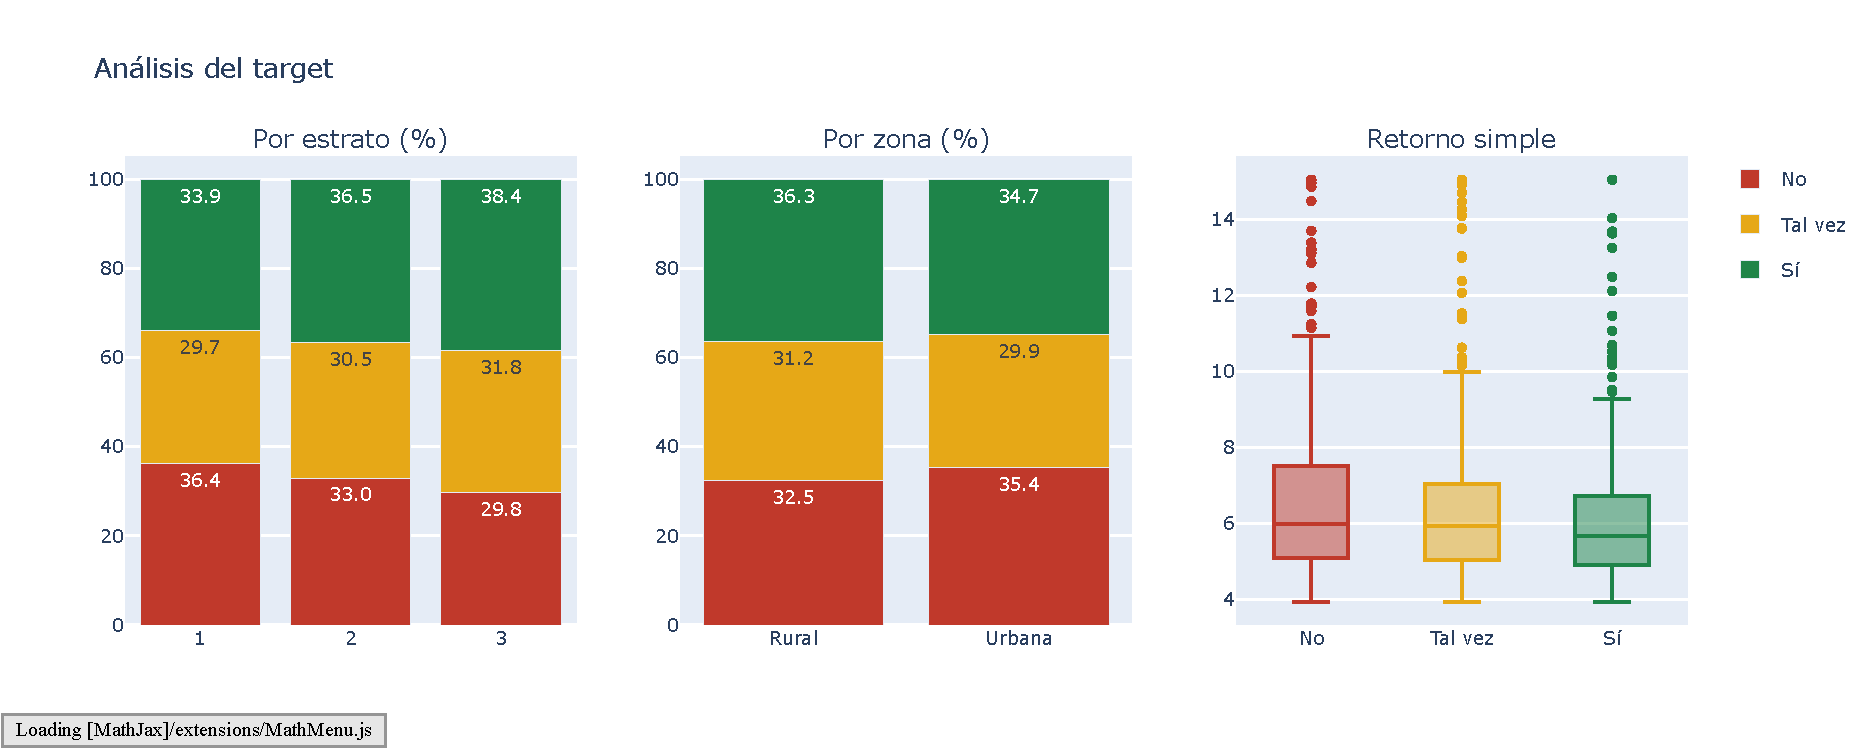
\includegraphics[width=\columnwidth]{figuras_gradio/analisis_target}\par}
{\par\centering\small\textbf{Figura~G.1:} Análisis: target.\par\vspace{0.8em}}
{\par\centering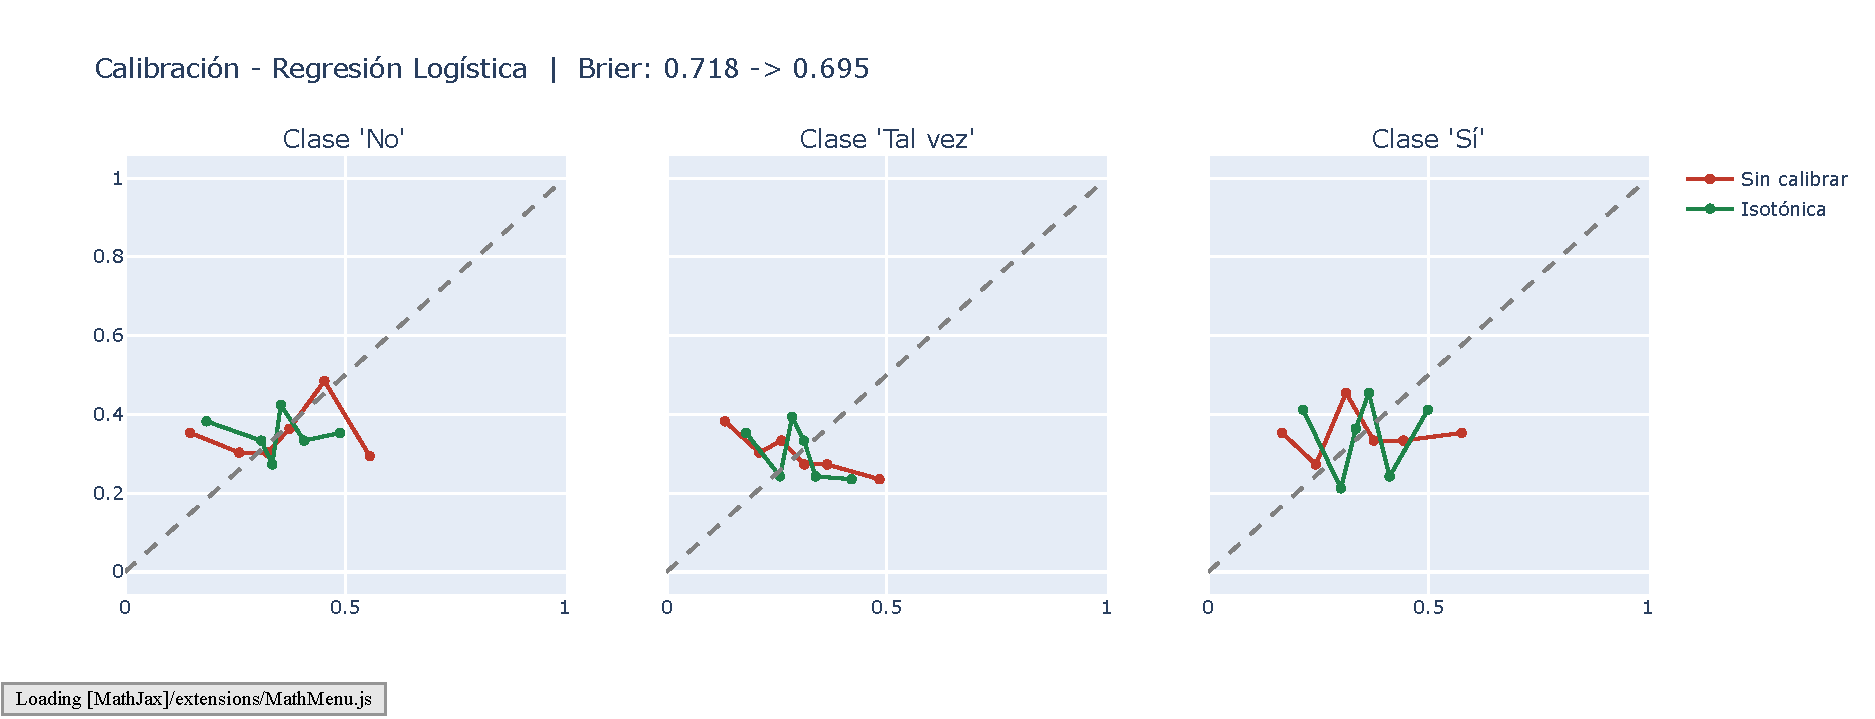
\includegraphics[width=\columnwidth]{figuras_gradio/clf_calibracion}\par}
{\par\centering\small\textbf{Figura~G.2:} Clasificador: calibracion.\par\vspace{0.8em}}
{\par\centering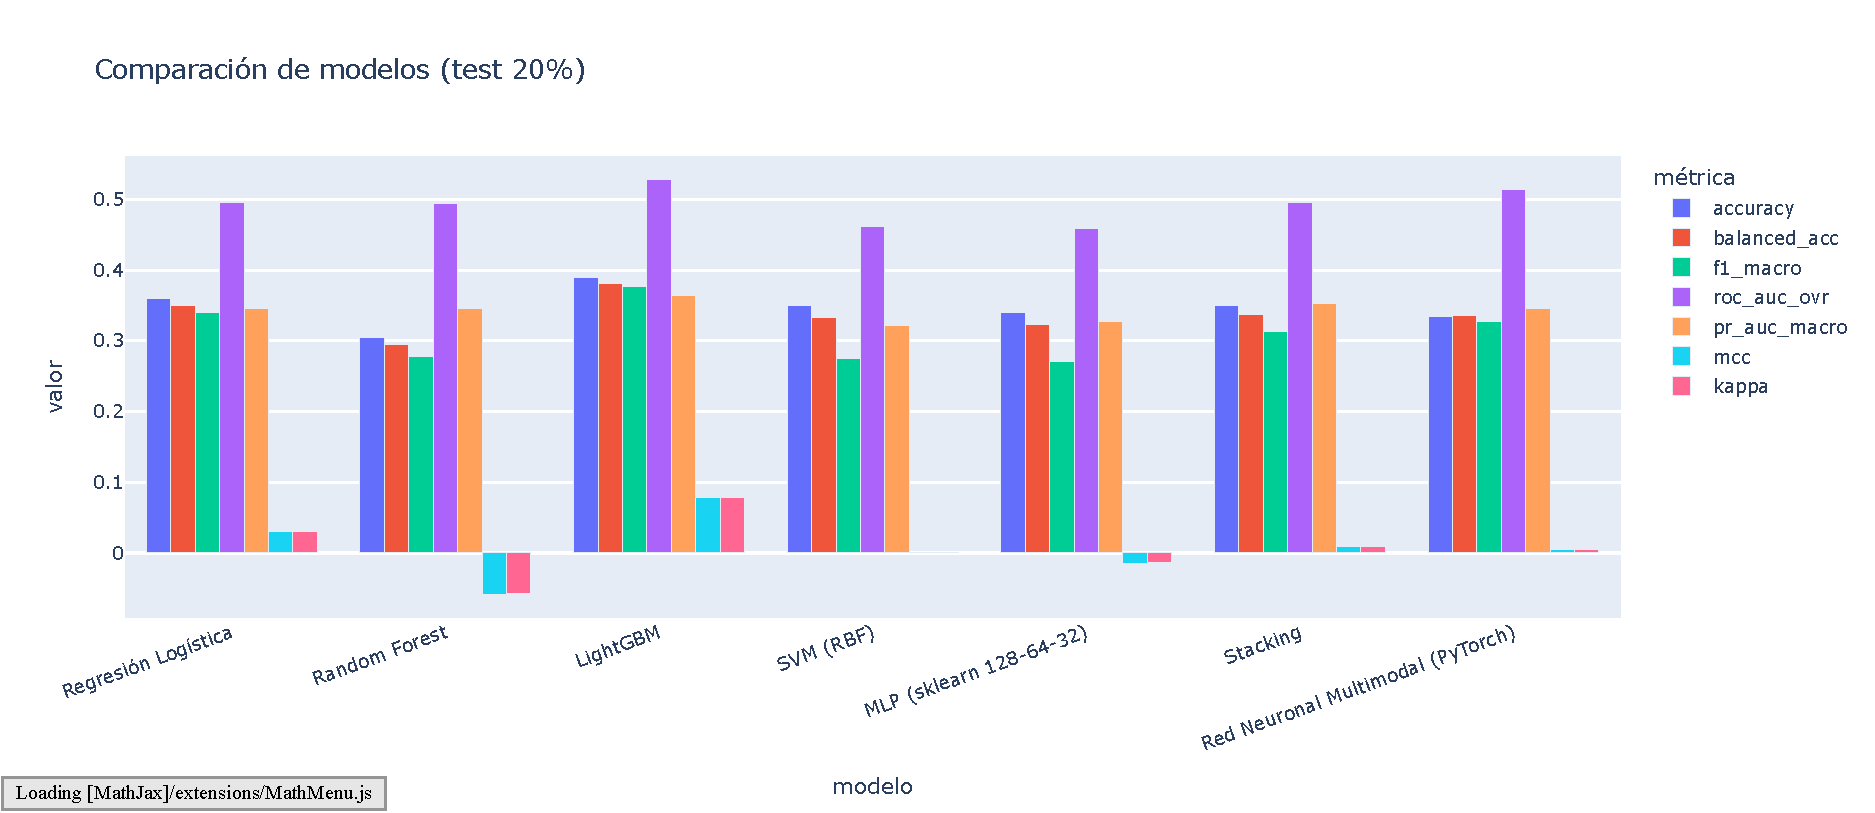
\includegraphics[width=\columnwidth]{figuras_gradio/clf_comparacion_modelos}\par}
{\par\centering\small\textbf{Figura~G.3:} Clasificador: comparacion modelos.\par\vspace{0.8em}}
{\par\centering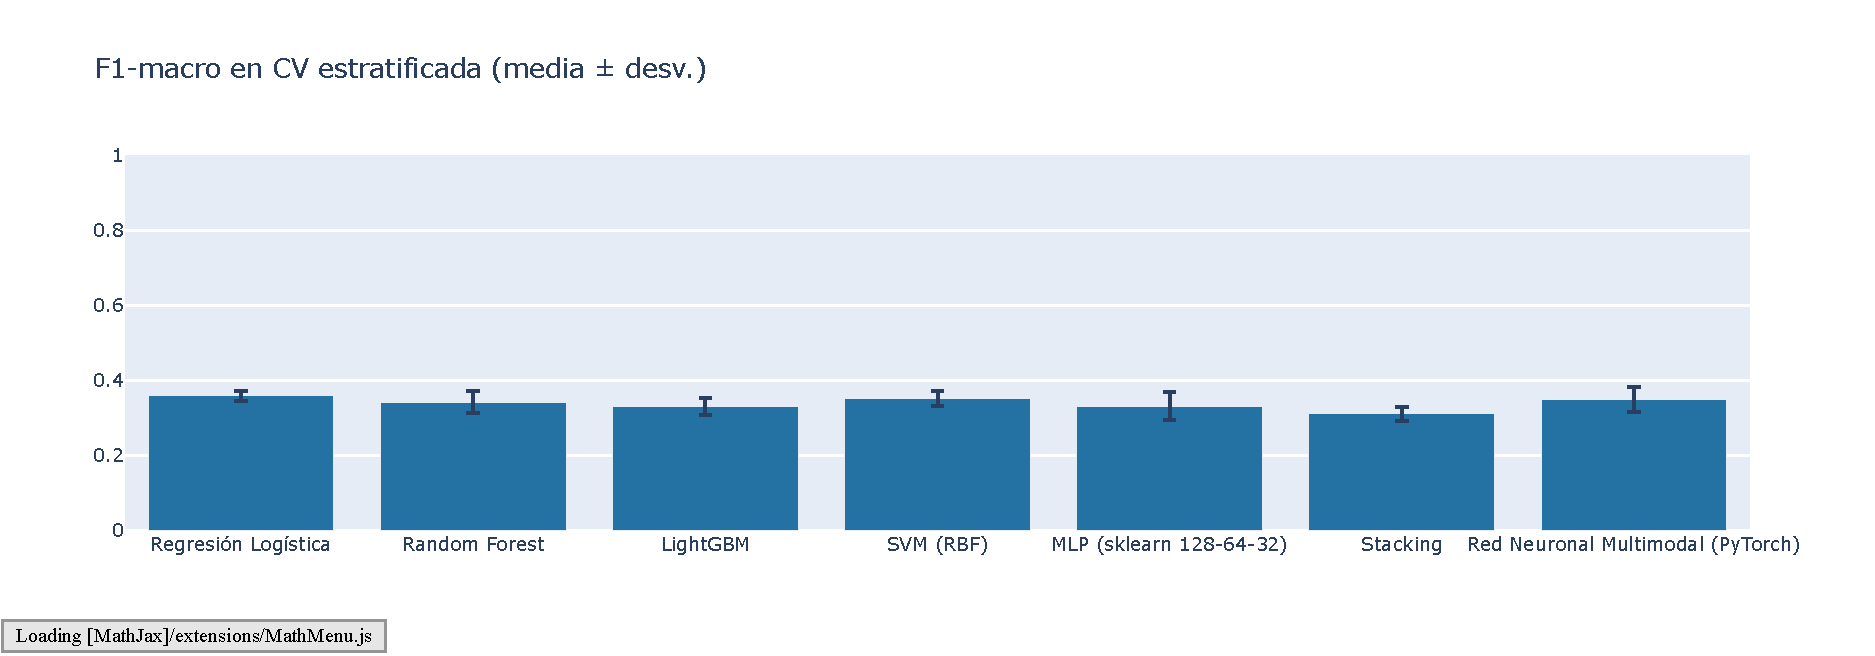
\includegraphics[width=\columnwidth]{figuras_gradio/clf_cv_f1}\par}
{\par\centering\small\textbf{Figura~G.4:} Clasificador: cv f1.\par\vspace{0.8em}}
{\par\centering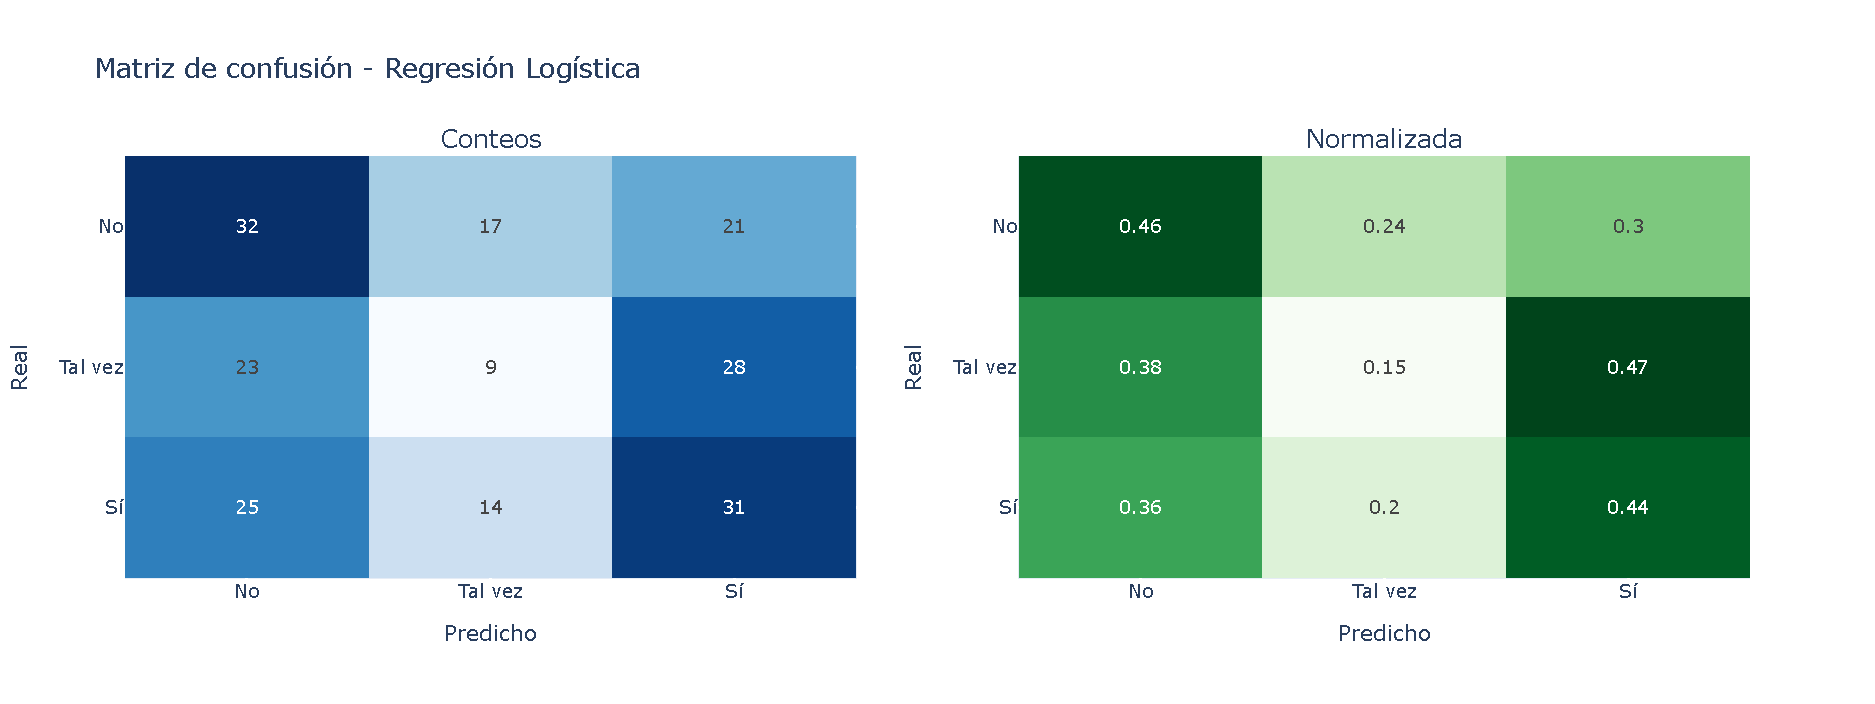
\includegraphics[width=\columnwidth]{figuras_gradio/clf_matriz_confusion}\par}
{\par\centering\small\textbf{Figura~G.5:} Clasificador: matriz confusion.\par\vspace{0.8em}}
{\par\centering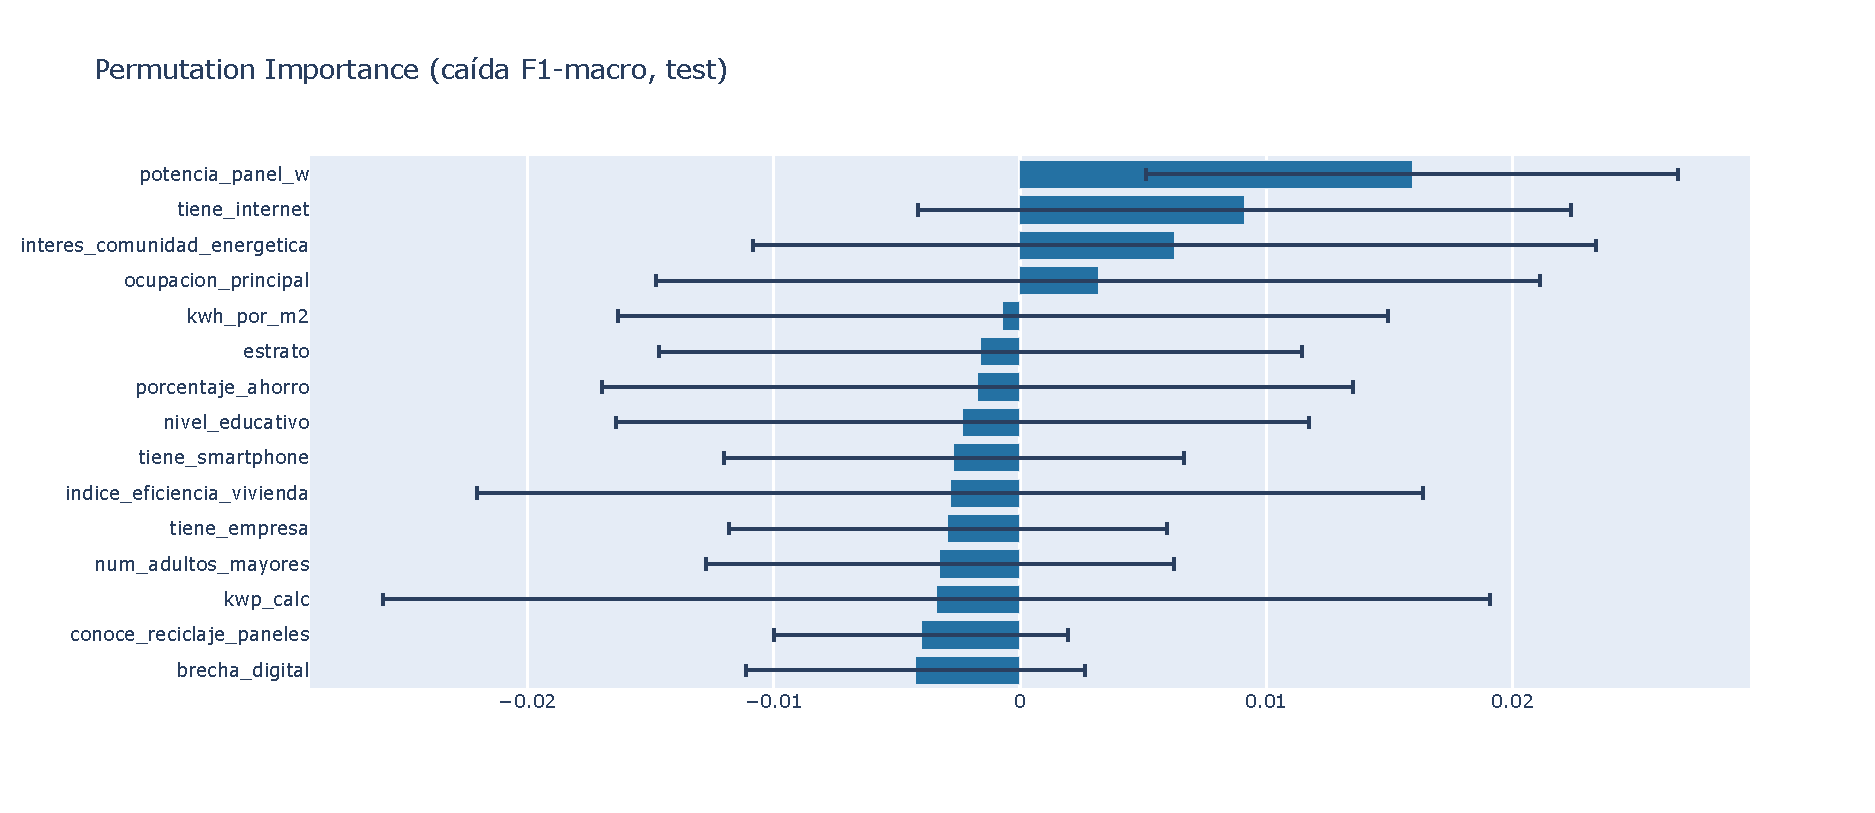
\includegraphics[width=\columnwidth]{figuras_gradio/clf_permutation_importance}\par}
{\par\centering\small\textbf{Figura~G.6:} Clasificador: permutation importance.\par\vspace{0.8em}}
{\par\centering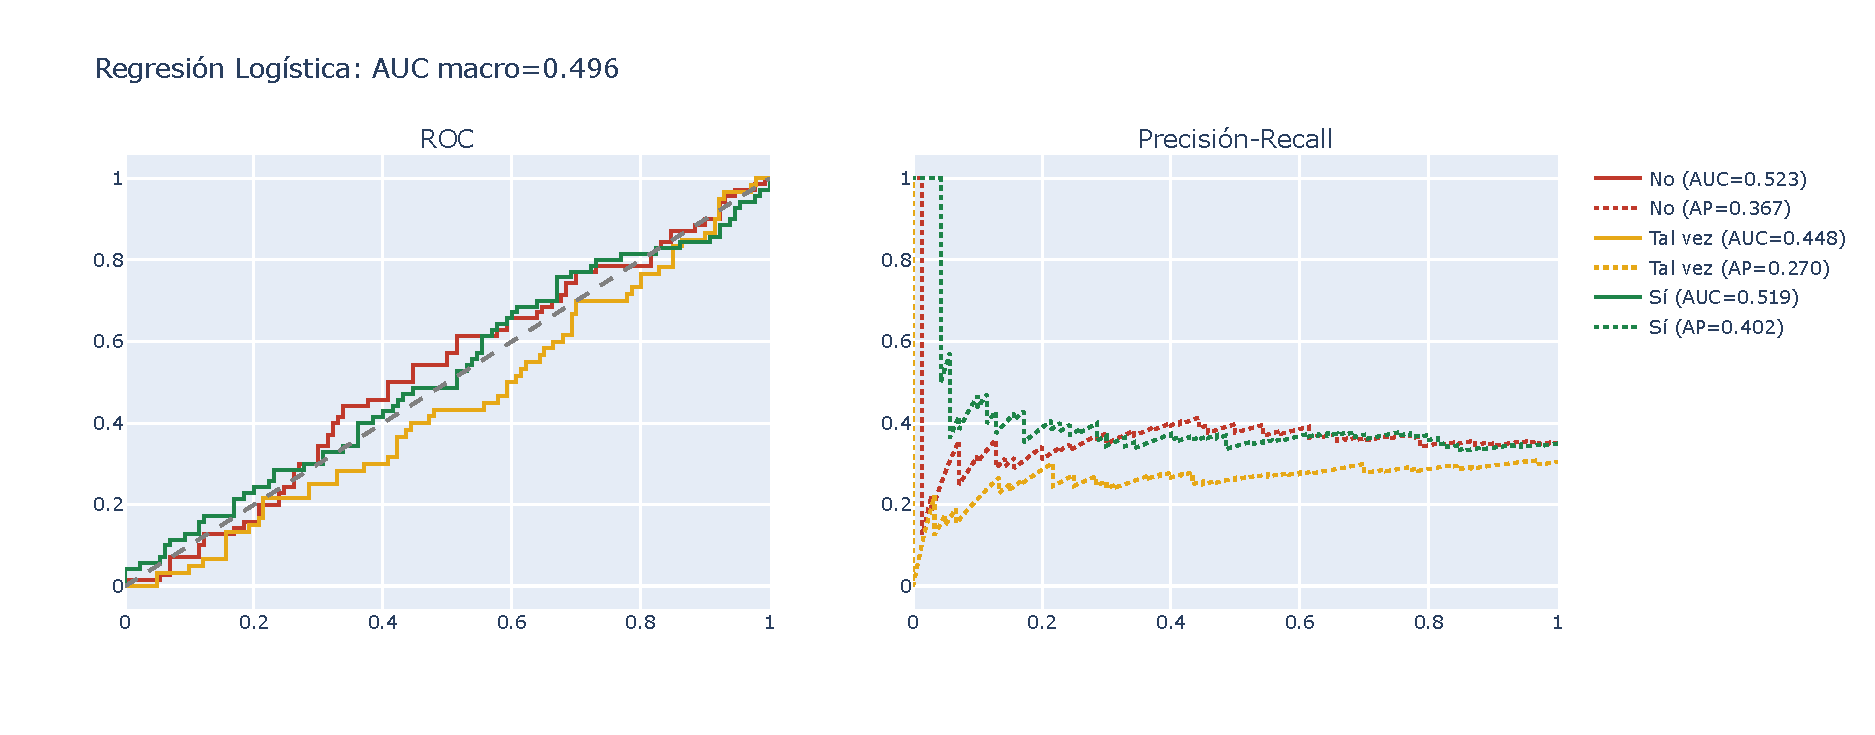
\includegraphics[width=\columnwidth]{figuras_gradio/clf_roc_pr}\par}
{\par\centering\small\textbf{Figura~G.7:} Clasificador: roc pr.\par\vspace{0.8em}}
{\par\centering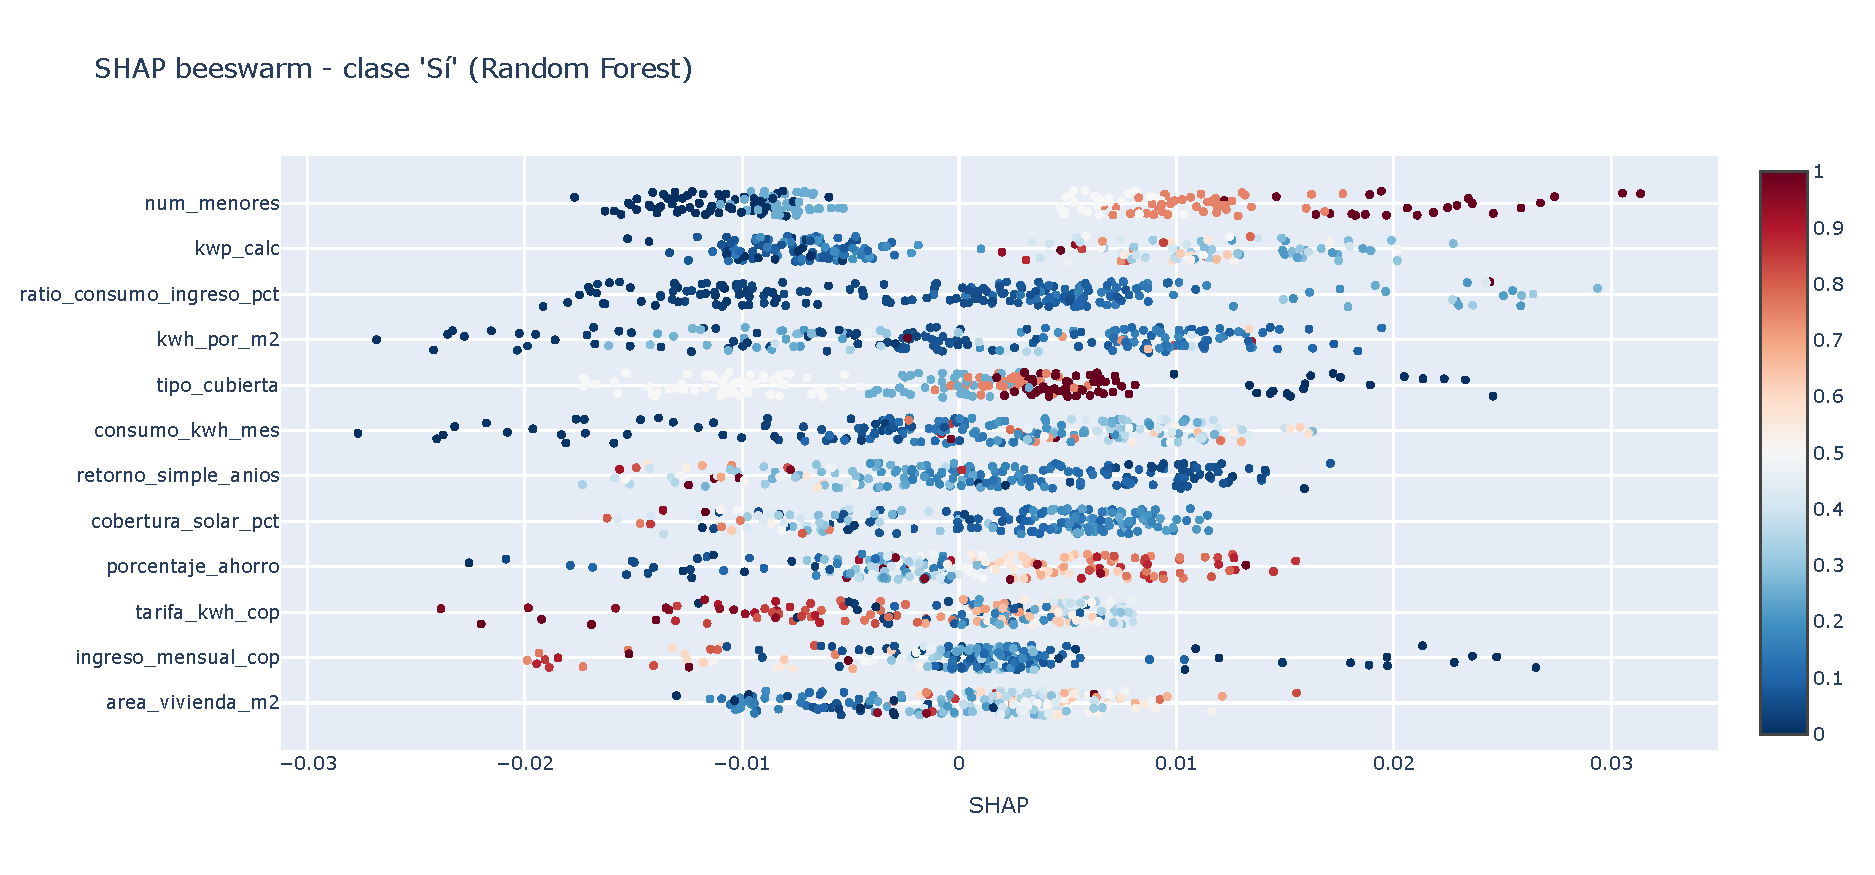
\includegraphics[width=\columnwidth]{figuras_gradio/clf_shap_beeswarm_si}\par}
{\par\centering\small\textbf{Figura~G.8:} Clasificador: shap beeswarm si.\par\vspace{0.8em}}
{\par\centering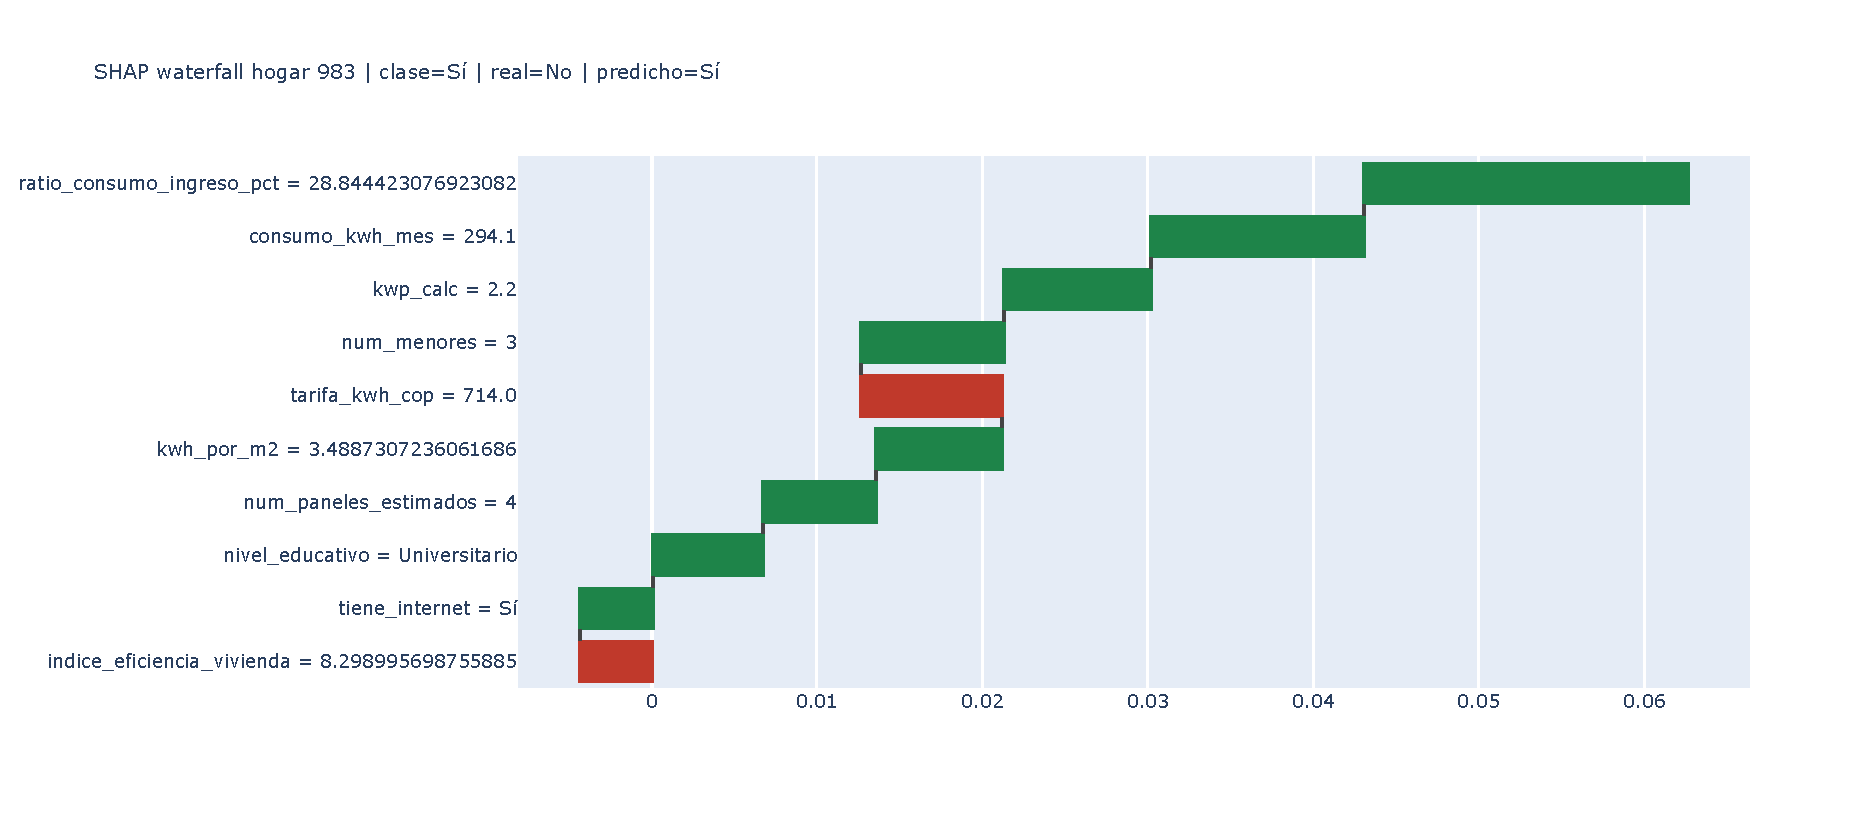
\includegraphics[width=\columnwidth]{figuras_gradio/clf_shap_force_ejemplo}\par}
{\par\centering\small\textbf{Figura~G.9:} Clasificador: shap force ejemplo.\par\vspace{0.8em}}
{\par\centering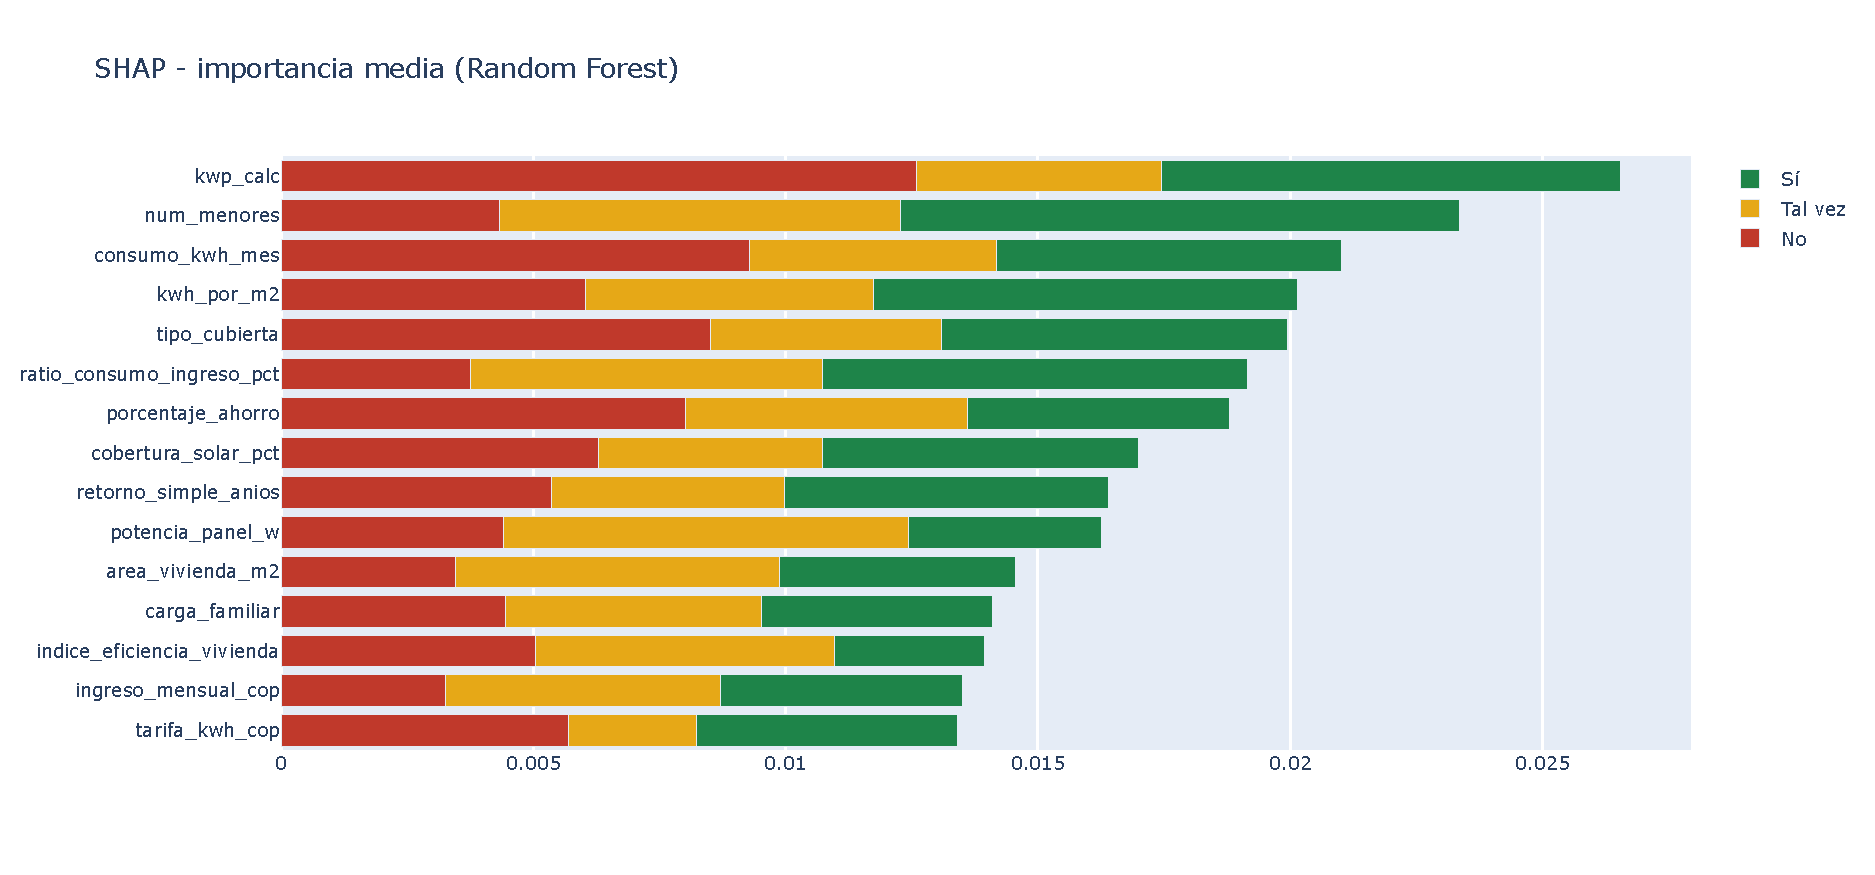
\includegraphics[width=\columnwidth]{figuras_gradio/clf_shap_resumen}\par}
{\par\centering\small\textbf{Figura~G.10:} Clasificador: shap resumen.\par\vspace{0.8em}}
{\par\centering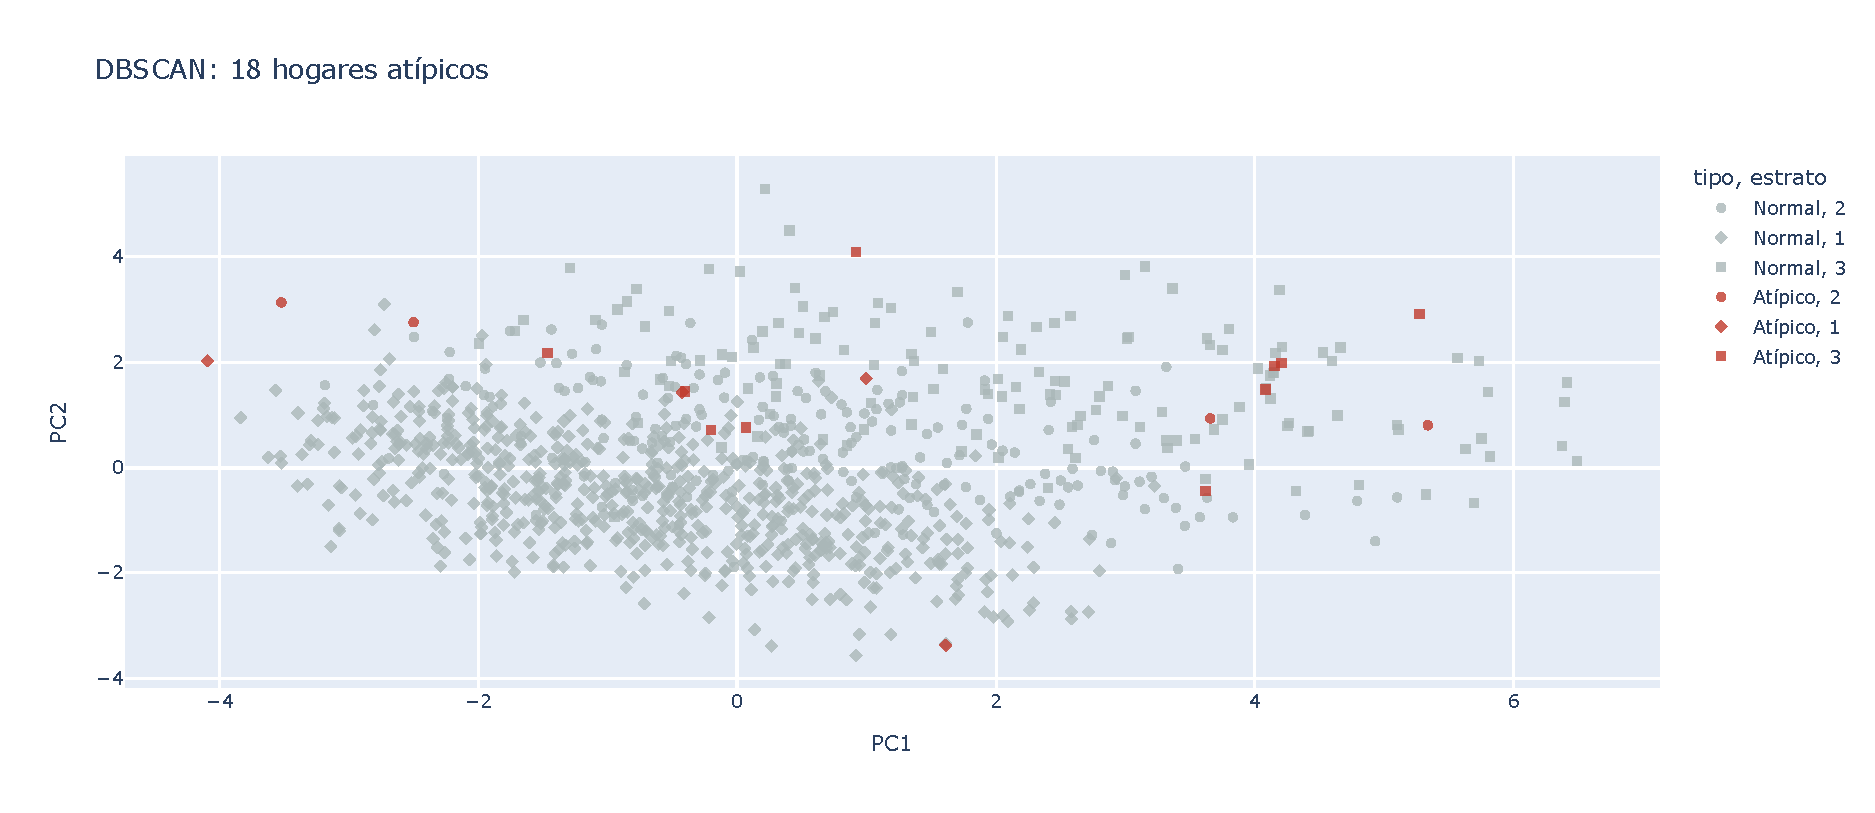
\includegraphics[width=\columnwidth]{figuras_gradio/dbscan_atipicos}\par}
{\par\centering\small\textbf{Figura~G.11:} Dbscan: atipicos.\par\vspace{0.8em}}
{\par\centering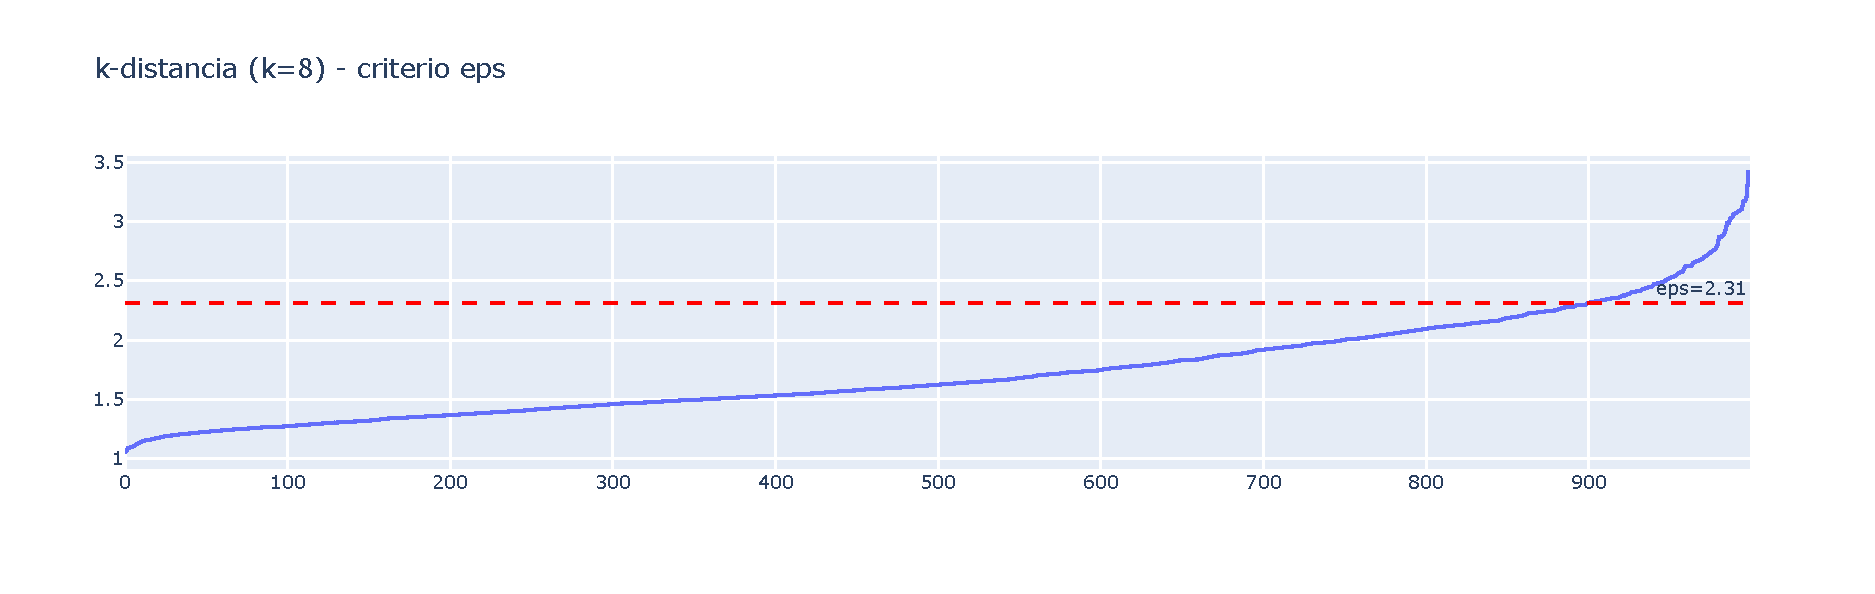
\includegraphics[width=\columnwidth]{figuras_gradio/dbscan_kdistancia}\par}
{\par\centering\small\textbf{Figura~G.12:} Dbscan: kdistancia.\par\vspace{0.8em}}
{\par\centering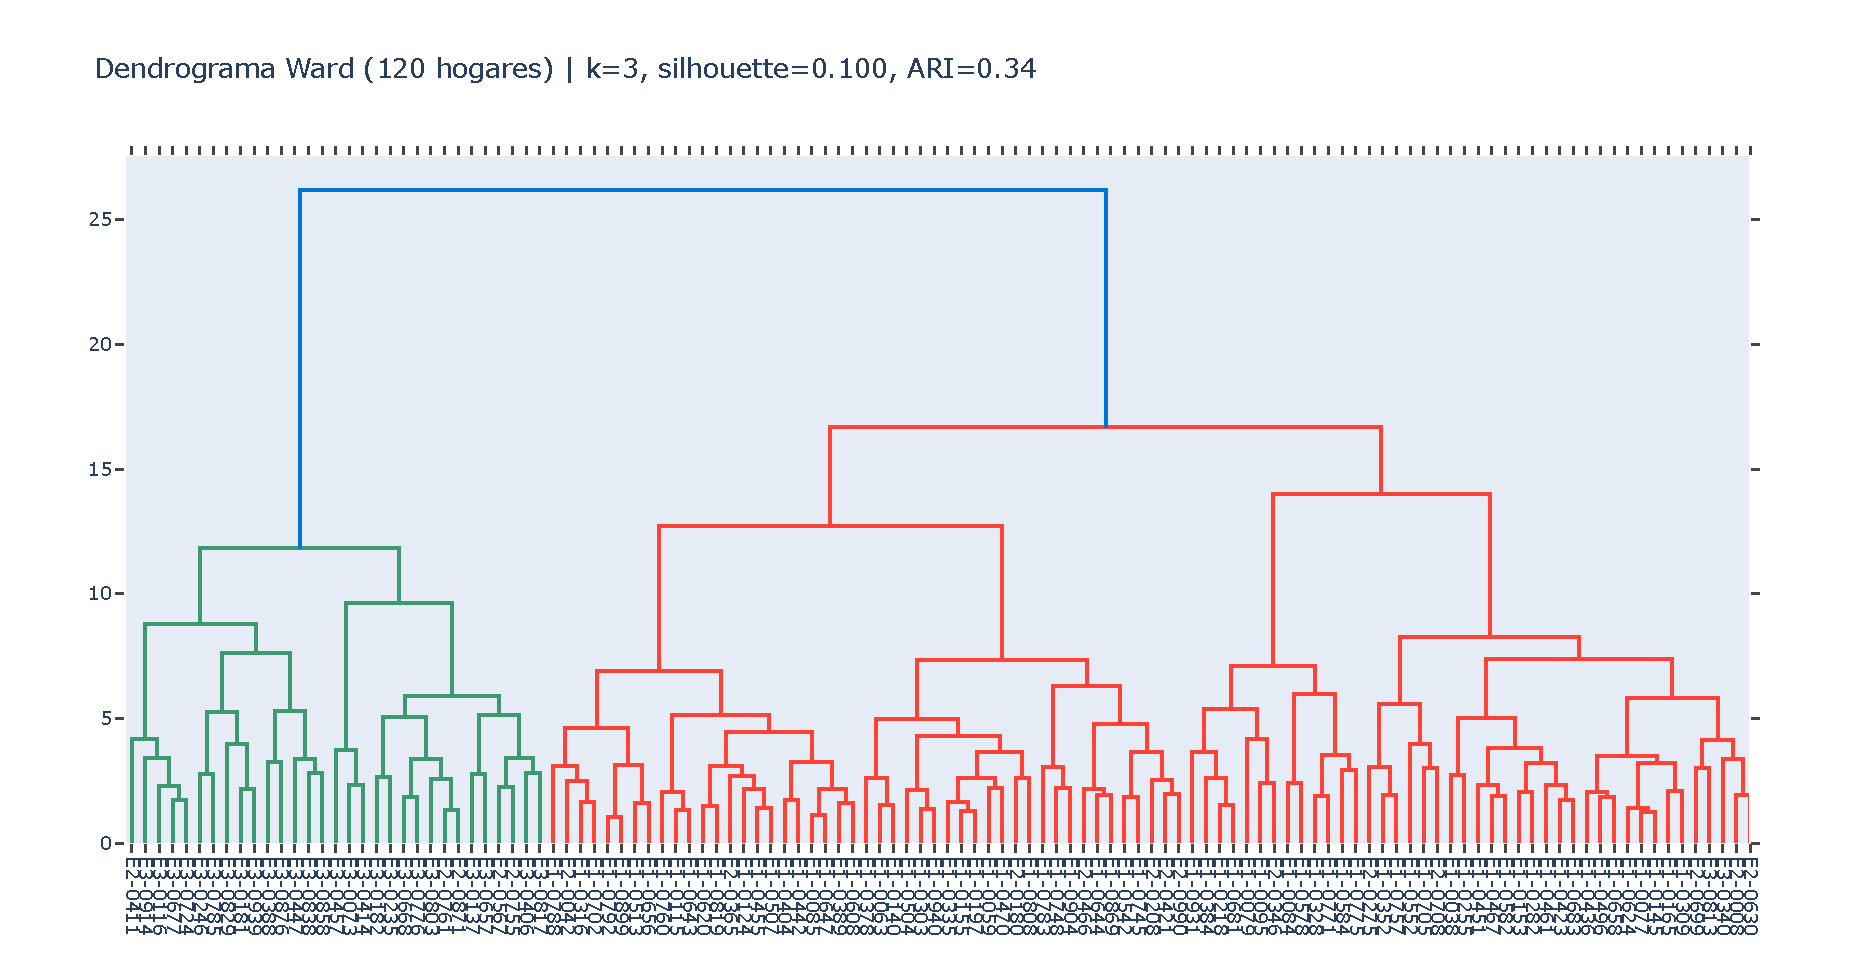
\includegraphics[width=\columnwidth]{figuras_gradio/dendrograma_clustering}\par}
{\par\centering\small\textbf{Figura~G.13:} Dendrograma: clustering.\par\vspace{0.8em}}
{\par\centering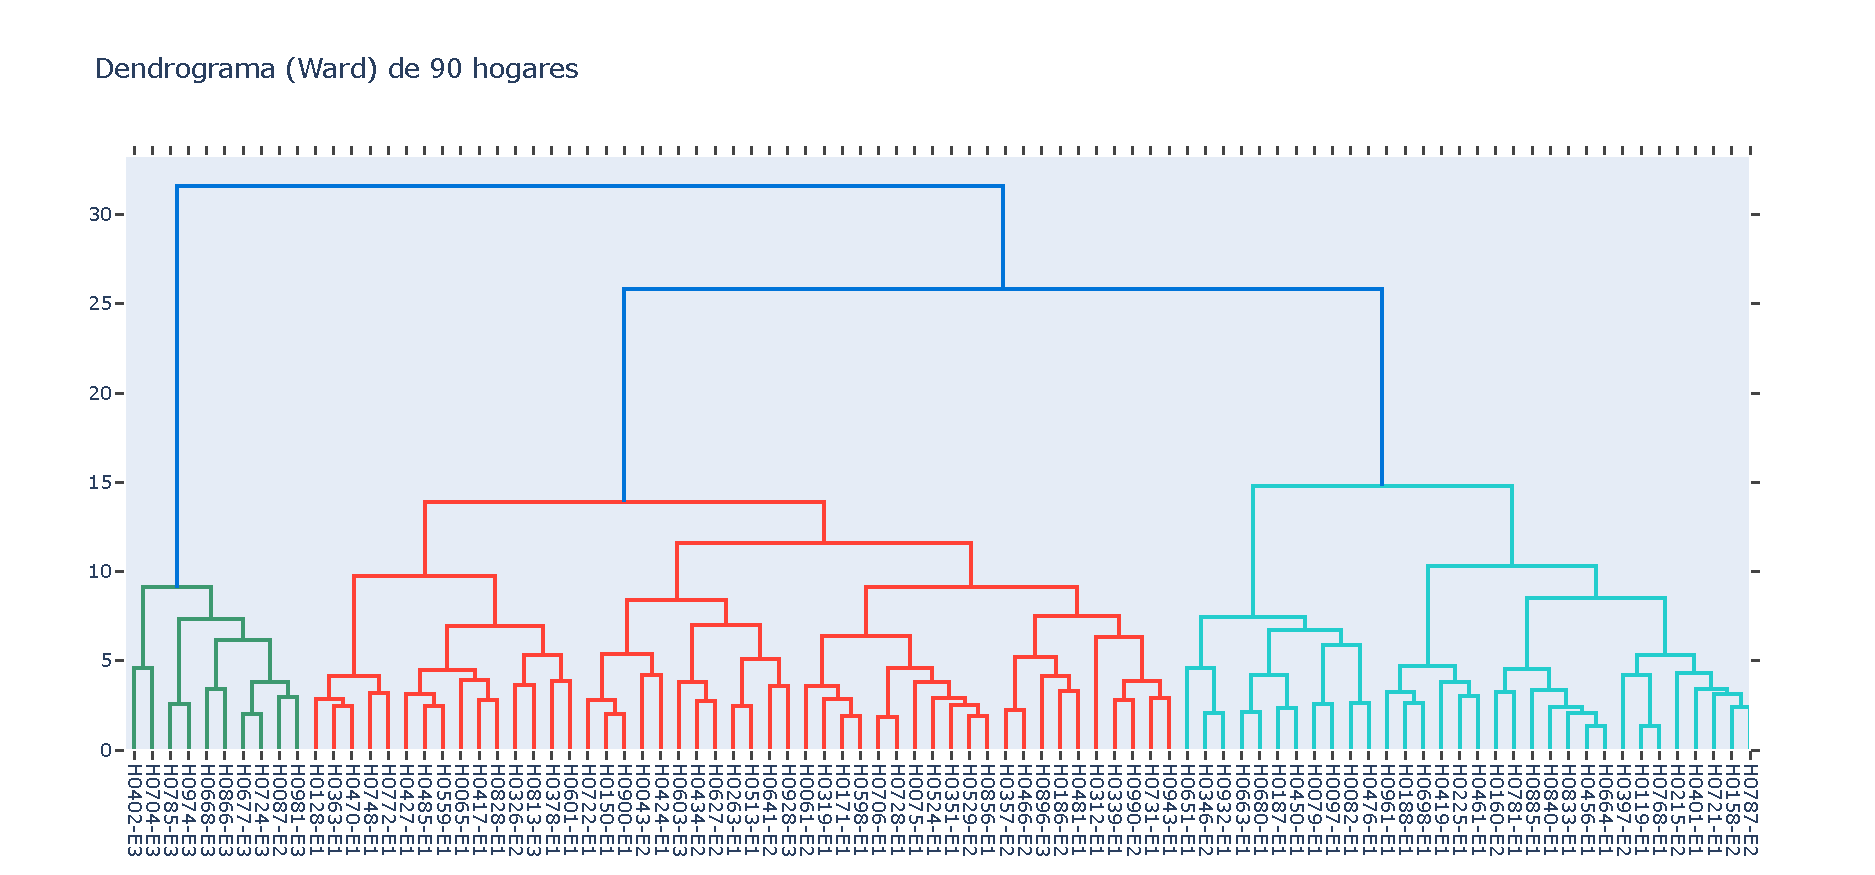
\includegraphics[width=\columnwidth]{figuras_gradio/dendrograma_eda}\par}
{\par\centering\small\textbf{Figura~G.14:} Dendrograma: eda.\par\vspace{0.8em}}
{\par\centering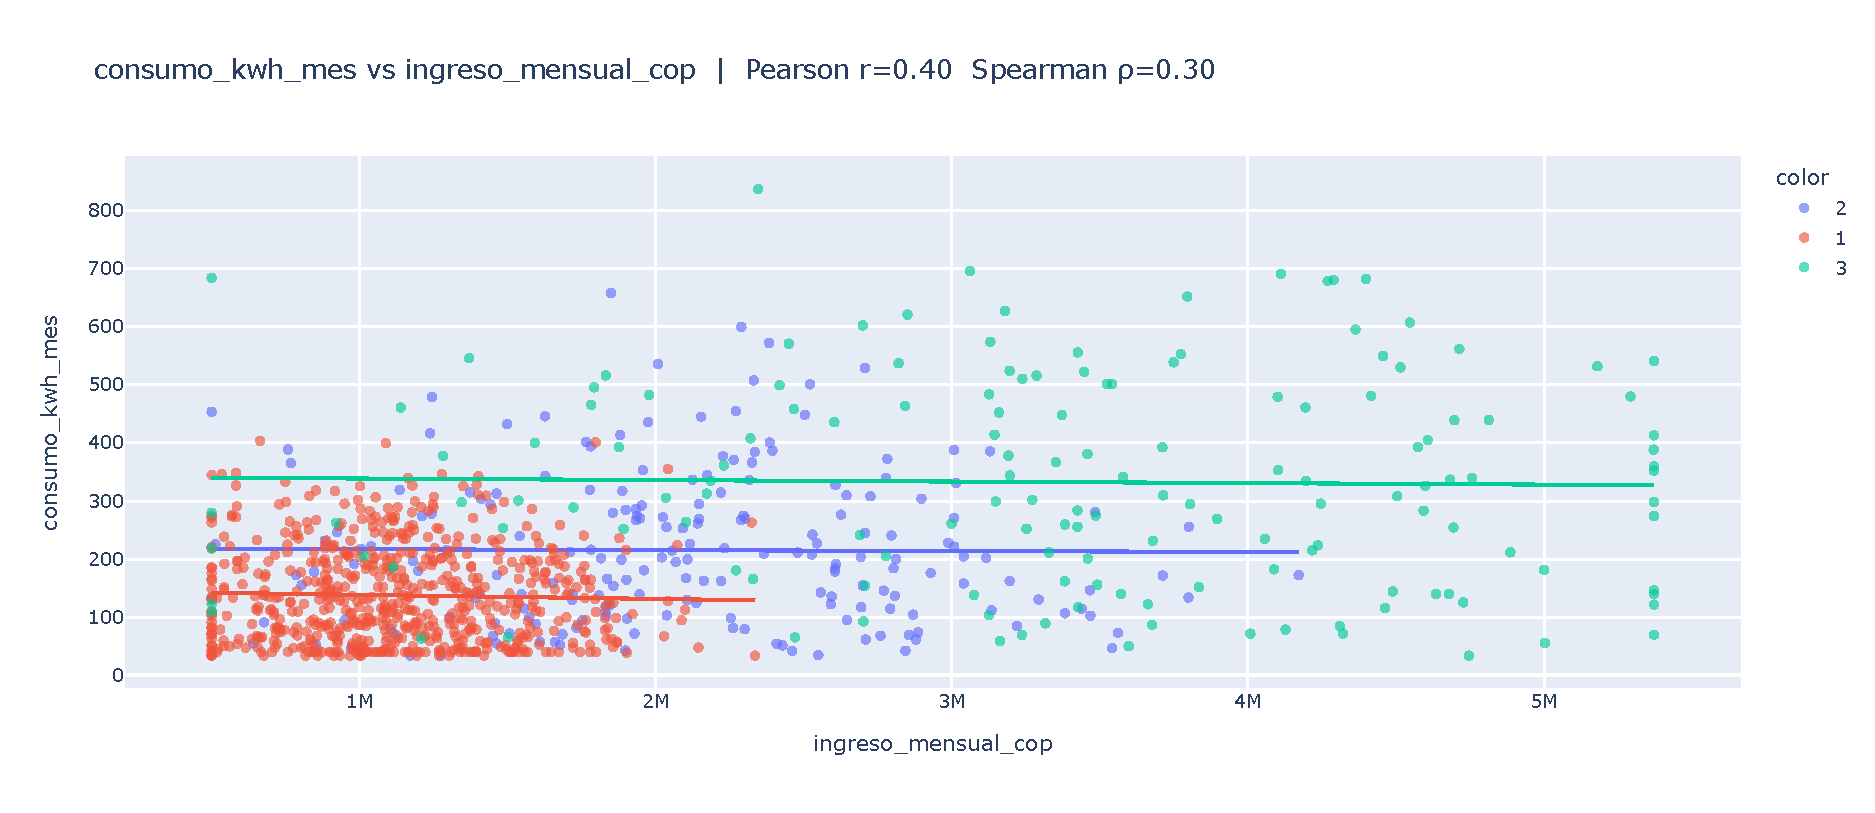
\includegraphics[width=\columnwidth]{figuras_gradio/eda_bivariado_consumo_ingreso}\par}
{\par\centering\small\textbf{Figura~G.15:} Eda: bivariado consumo ingreso.\par\vspace{0.8em}}
{\par\centering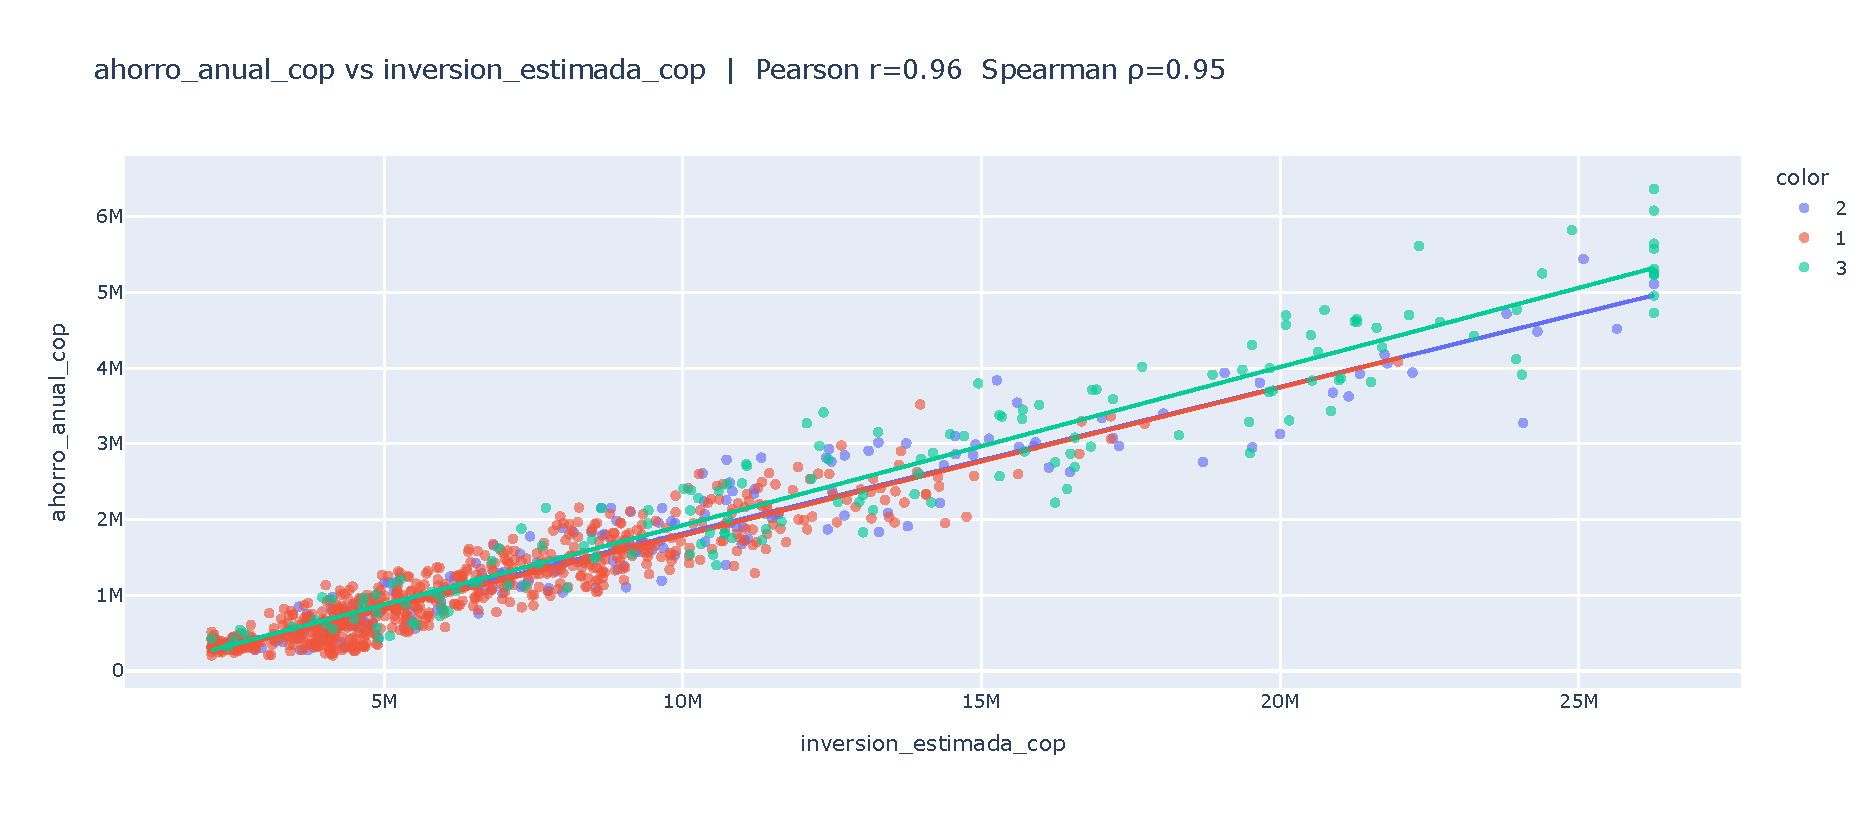
\includegraphics[width=\columnwidth]{figuras_gradio/eda_bivariado_inversion_ahorro}\par}
{\par\centering\small\textbf{Figura~G.16:} Eda: bivariado inversion ahorro.\par\vspace{0.8em}}
{\par\centering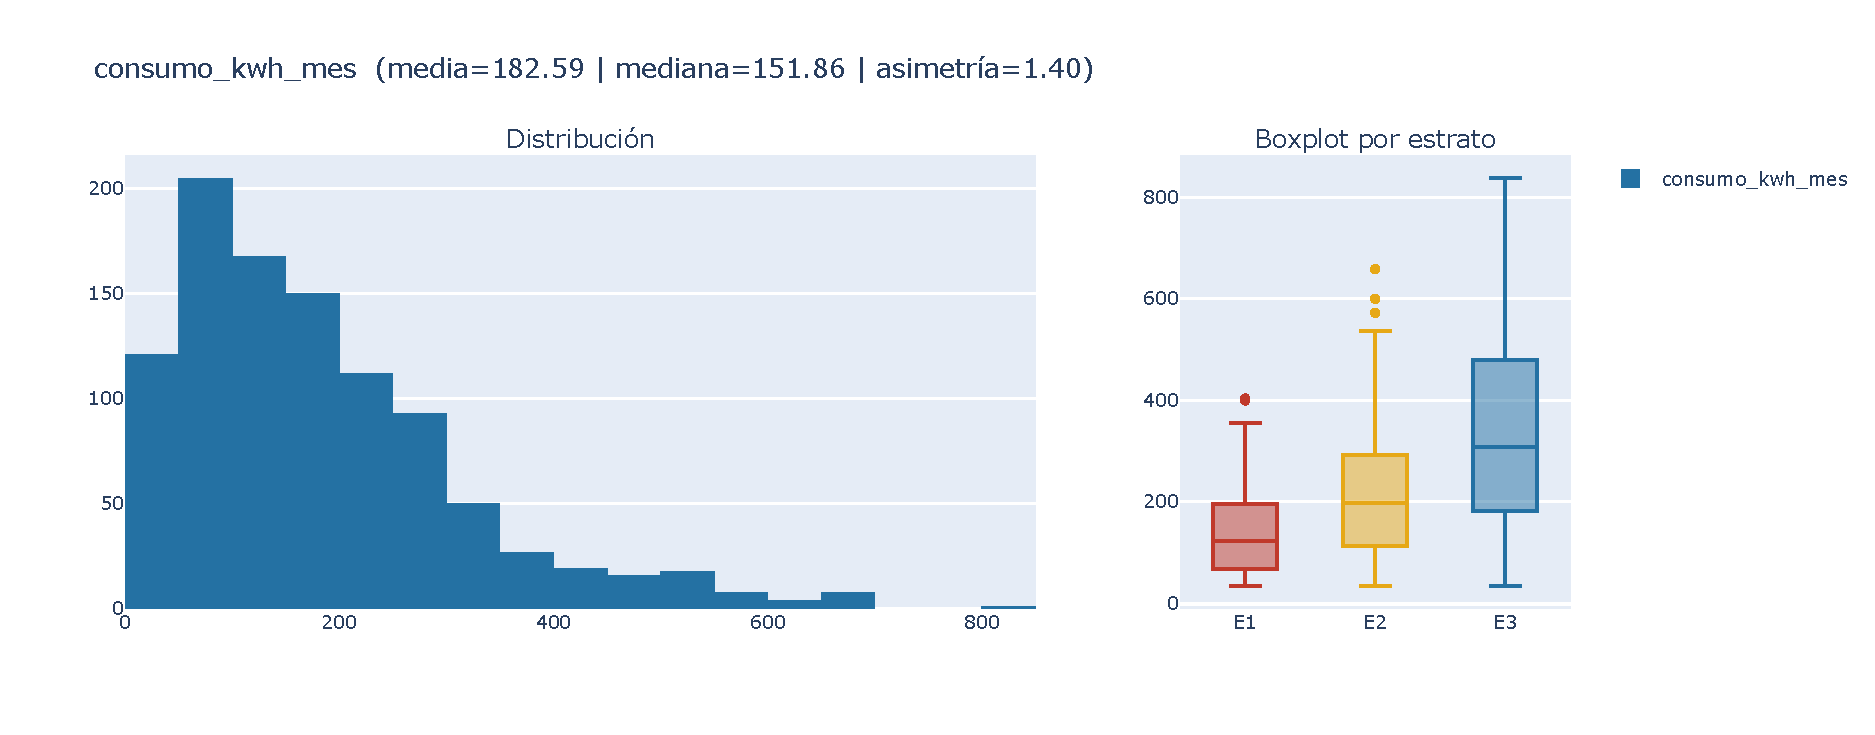
\includegraphics[width=\columnwidth]{figuras_gradio/eda_univariado_consumo_kwh_mes}\par}
{\par\centering\small\textbf{Figura~G.17:} Eda: univariado consumo kwh mes.\par\vspace{0.8em}}
{\par\centering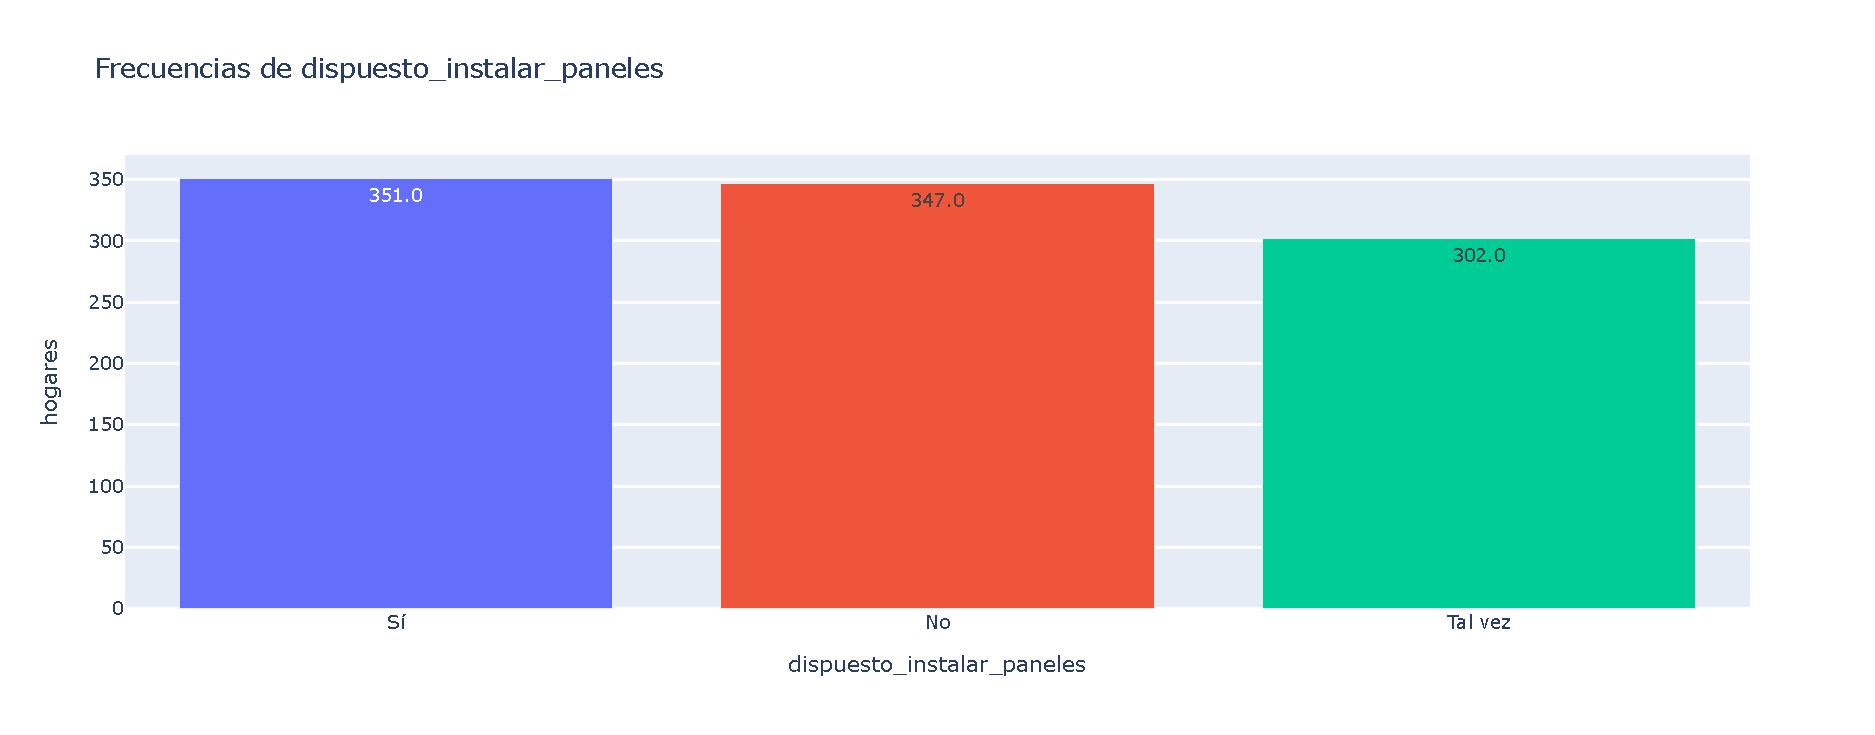
\includegraphics[width=\columnwidth]{figuras_gradio/eda_univariado_dispuesto_instalar_paneles}\par}
{\par\centering\small\textbf{Figura~G.18:} Eda: univariado dispuesto instalar paneles.\par\vspace{0.8em}}
{\par\centering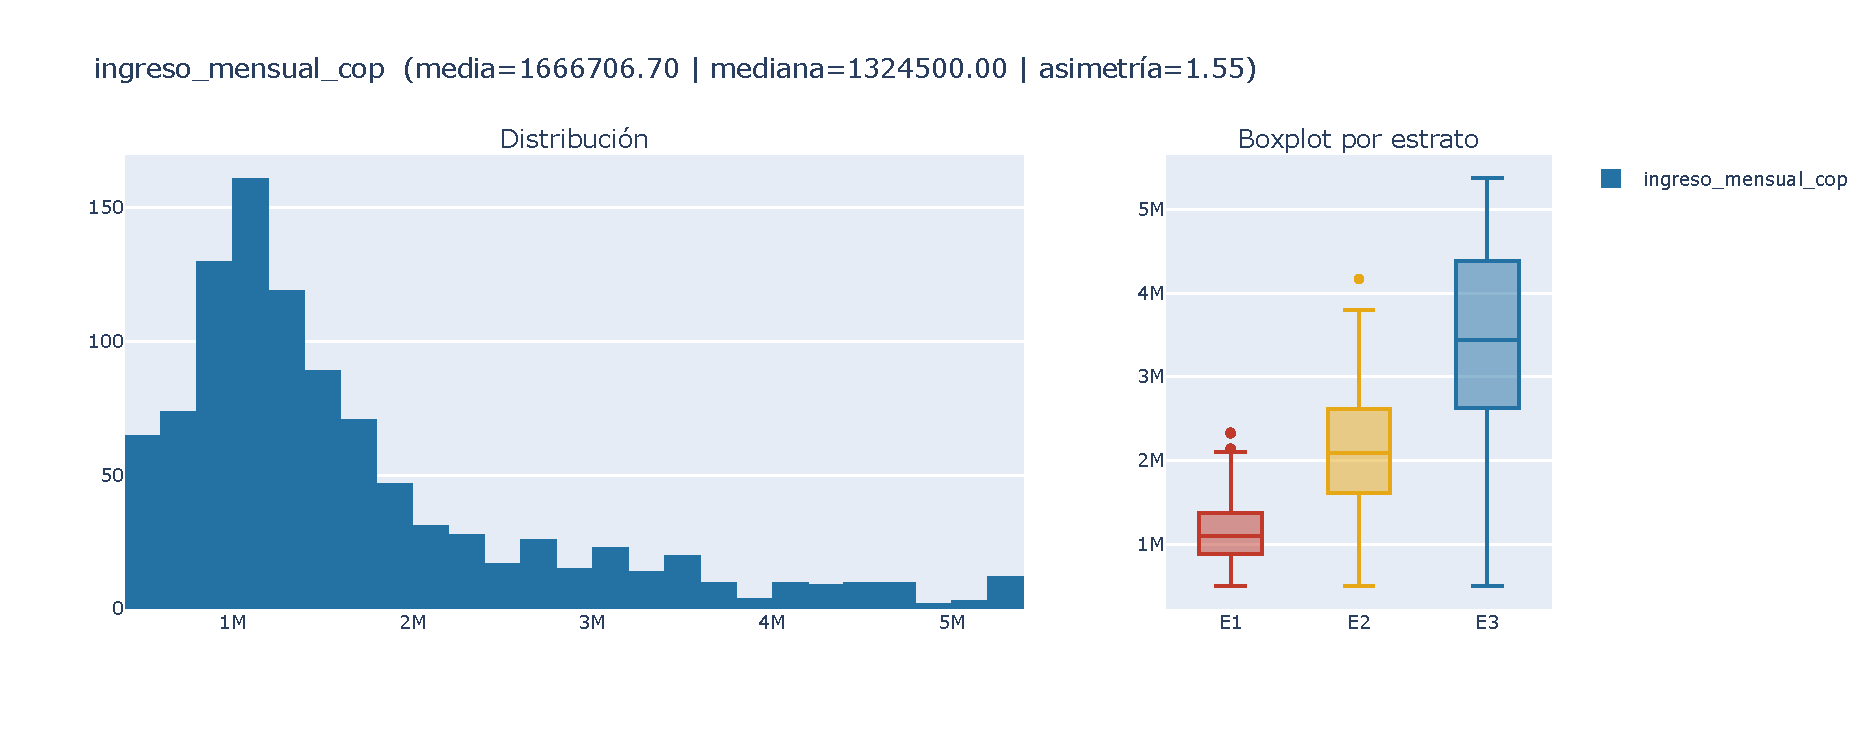
\includegraphics[width=\columnwidth]{figuras_gradio/eda_univariado_ingreso_mensual_cop}\par}
{\par\centering\small\textbf{Figura~G.19:} Eda: univariado ingreso mensual cop.\par\vspace{0.8em}}
{\par\centering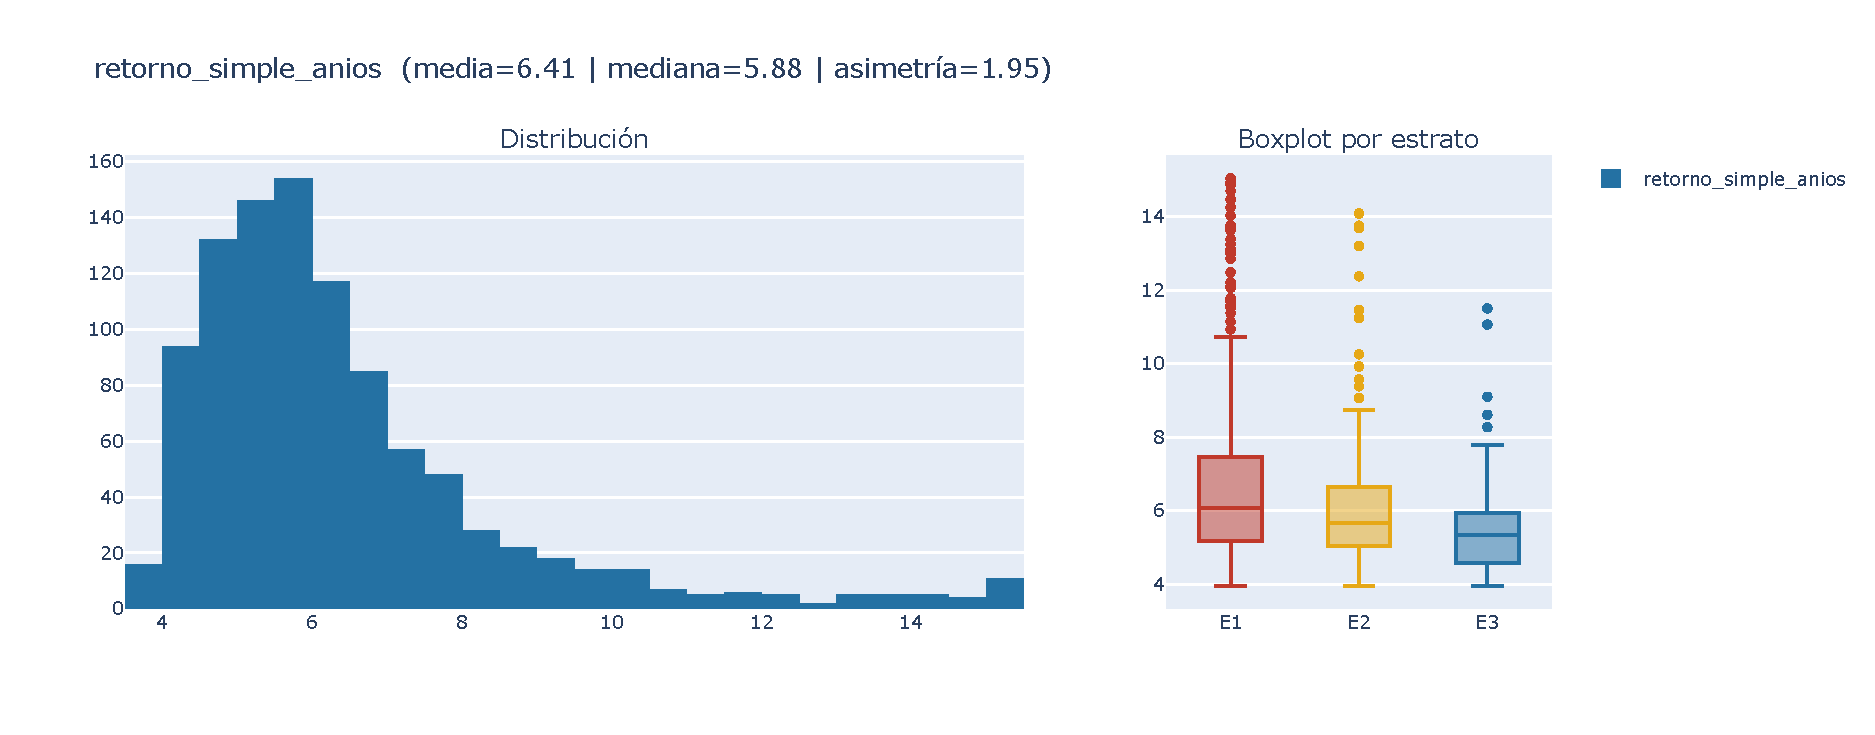
\includegraphics[width=\columnwidth]{figuras_gradio/eda_univariado_retorno_simple_anios}\par}
{\par\centering\small\textbf{Figura~G.20:} Eda: univariado retorno simple anios.\par\vspace{0.8em}}
{\par\centering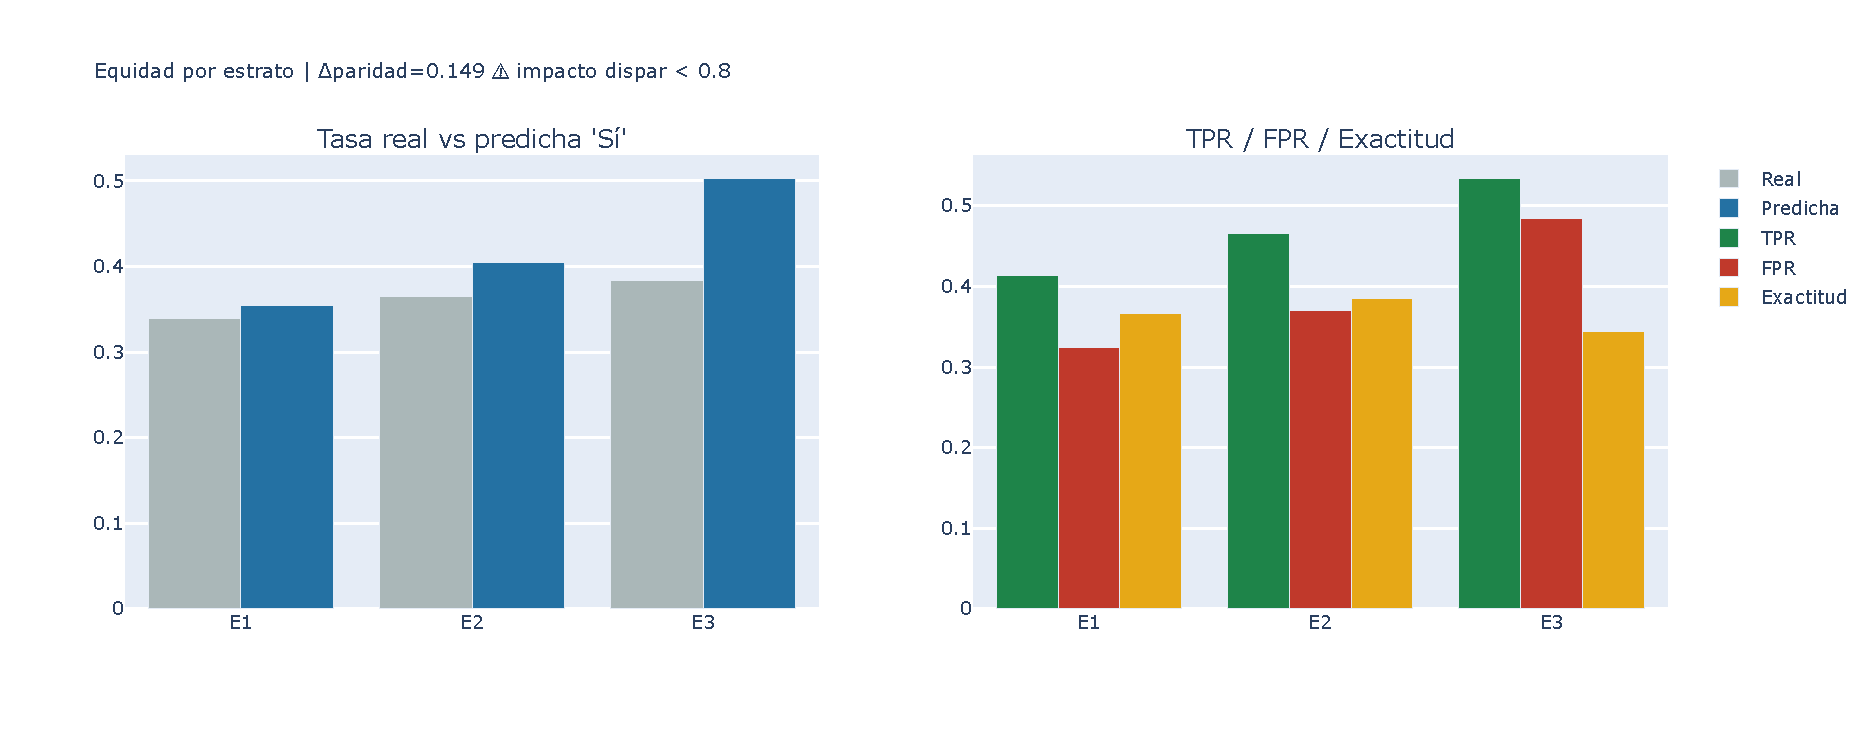
\includegraphics[width=\columnwidth]{figuras_gradio/fairness_estrato}\par}
{\par\centering\small\textbf{Figura~G.21:} Equidad: estrato.\par\vspace{0.8em}}
{\par\centering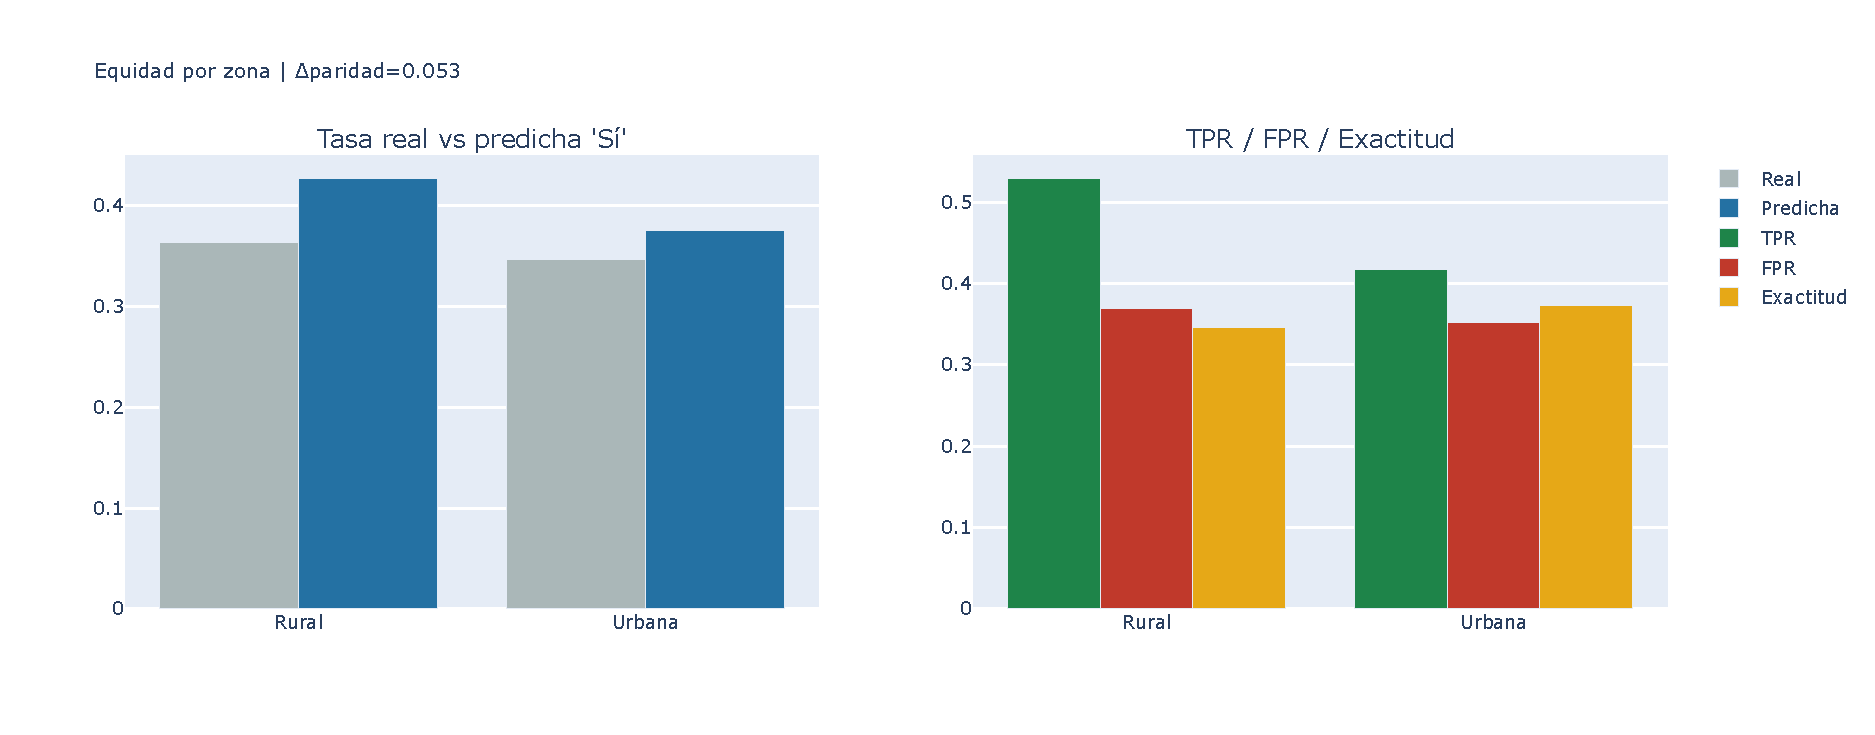
\includegraphics[width=\columnwidth]{figuras_gradio/fairness_zona}\par}
{\par\centering\small\textbf{Figura~G.22:} Equidad: zona.\par\vspace{0.8em}}
{\par\centering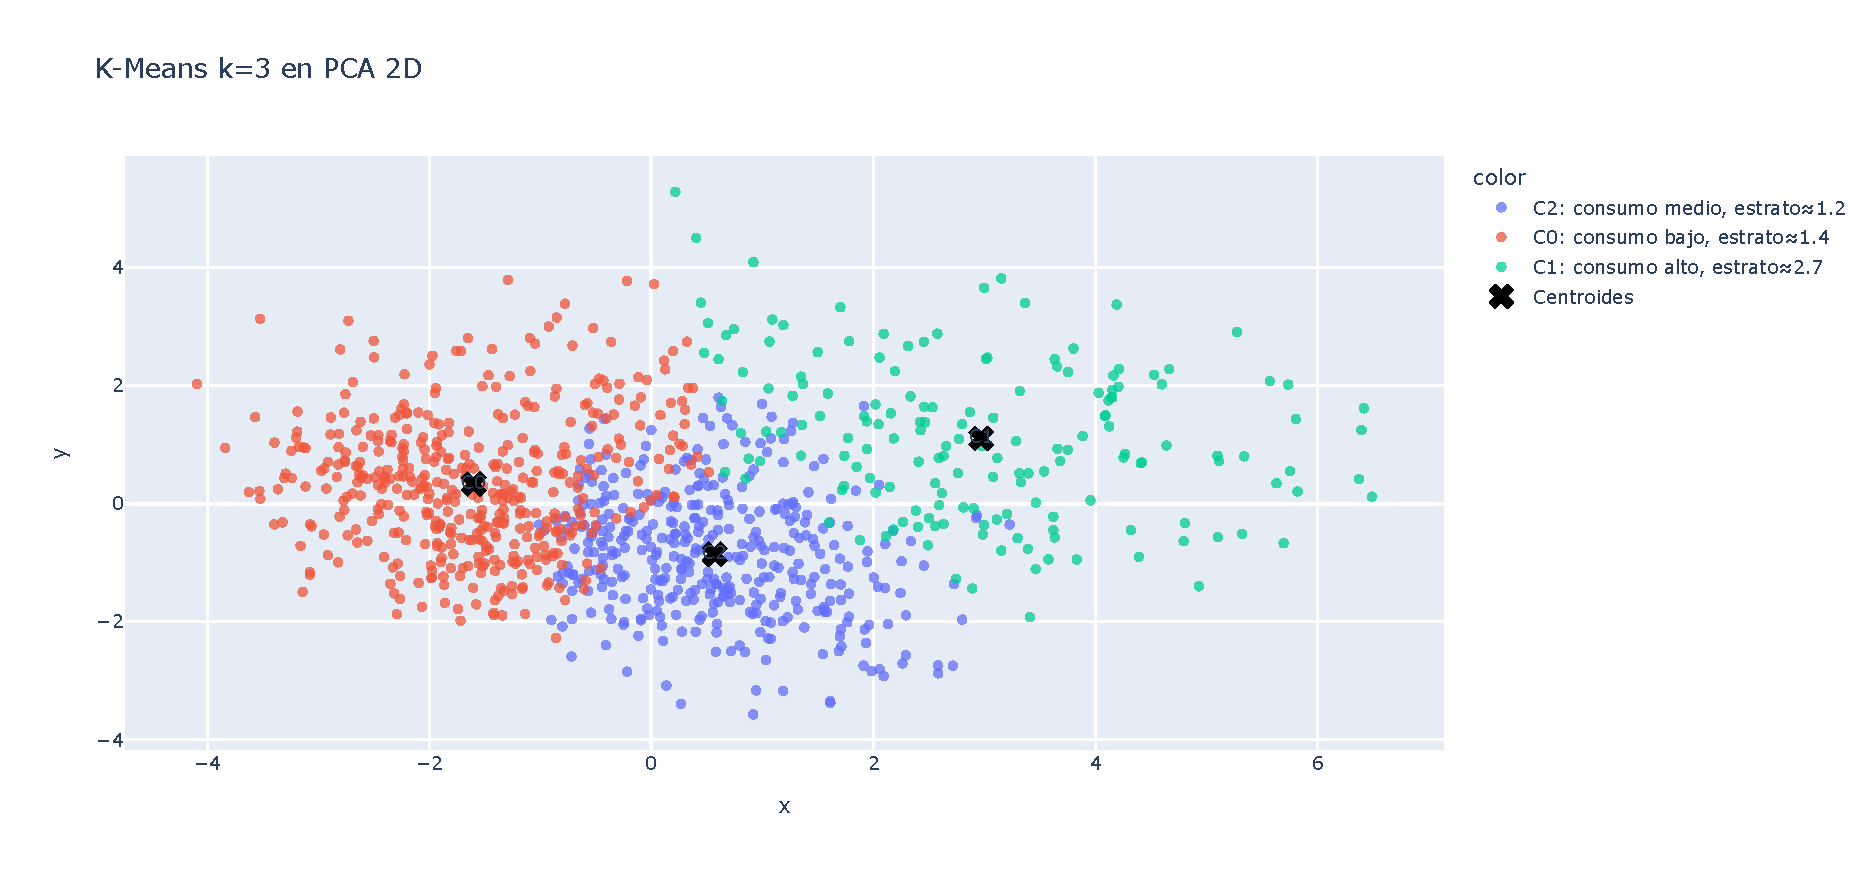
\includegraphics[width=\columnwidth]{figuras_gradio/kmeans_pca}\par}
{\par\centering\small\textbf{Figura~G.23:} K-means: pca.\par\vspace{0.8em}}
{\par\centering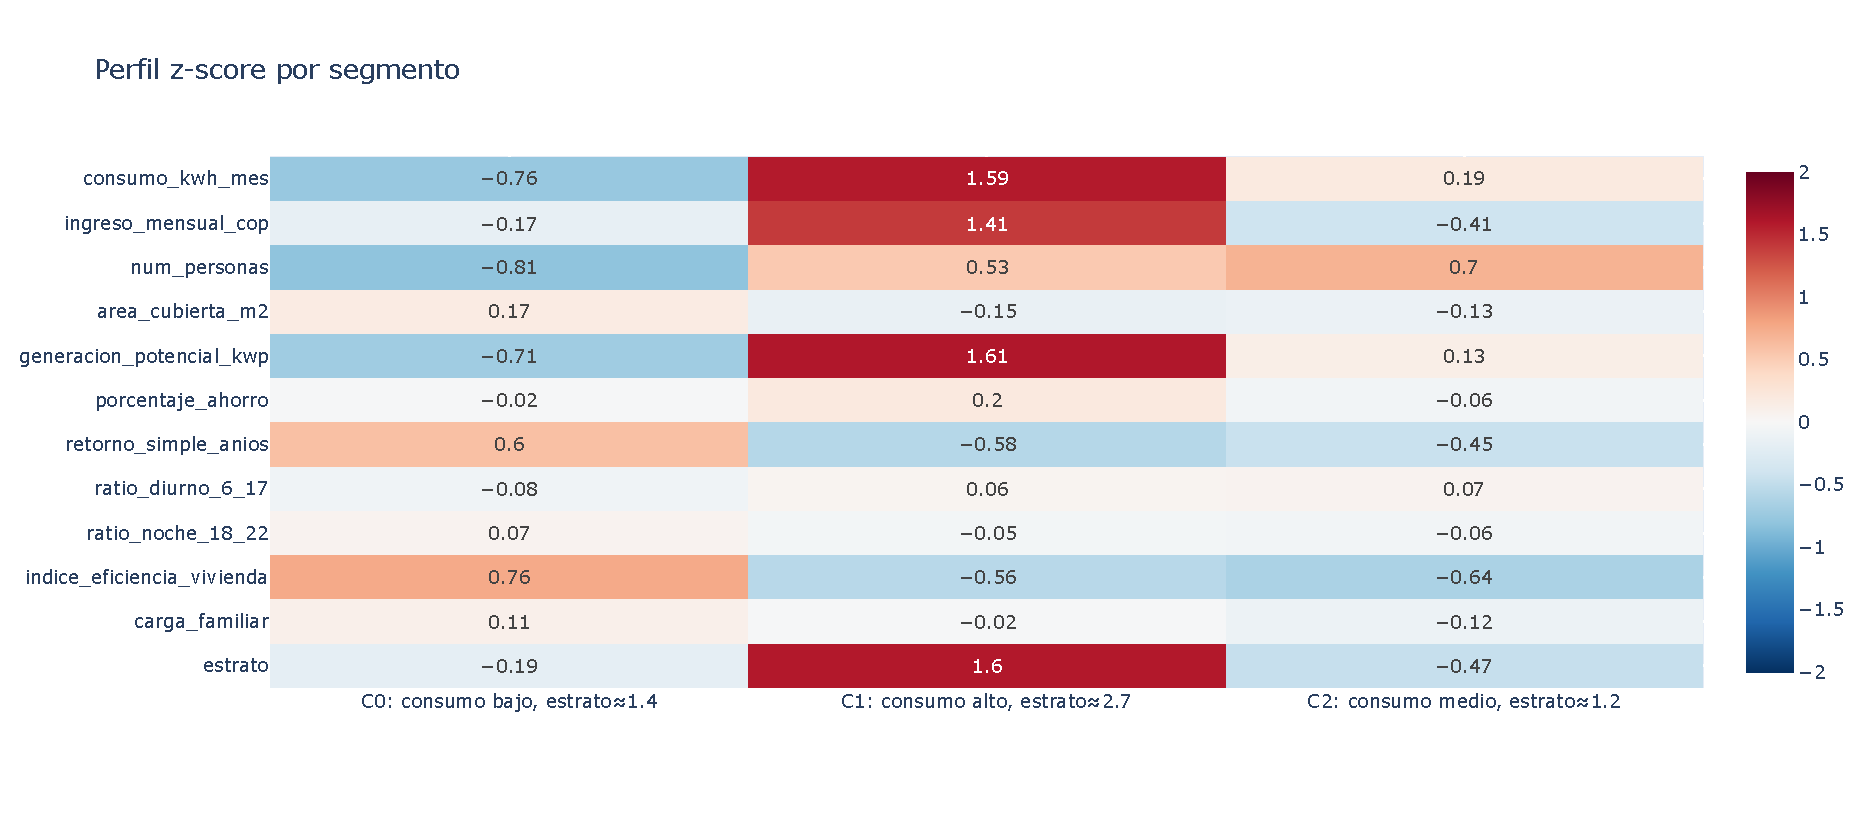
\includegraphics[width=\columnwidth]{figuras_gradio/kmeans_perfil_heatmap}\par}
{\par\centering\small\textbf{Figura~G.24:} K-means: perfil heatmap.\par\vspace{0.8em}}
{\par\centering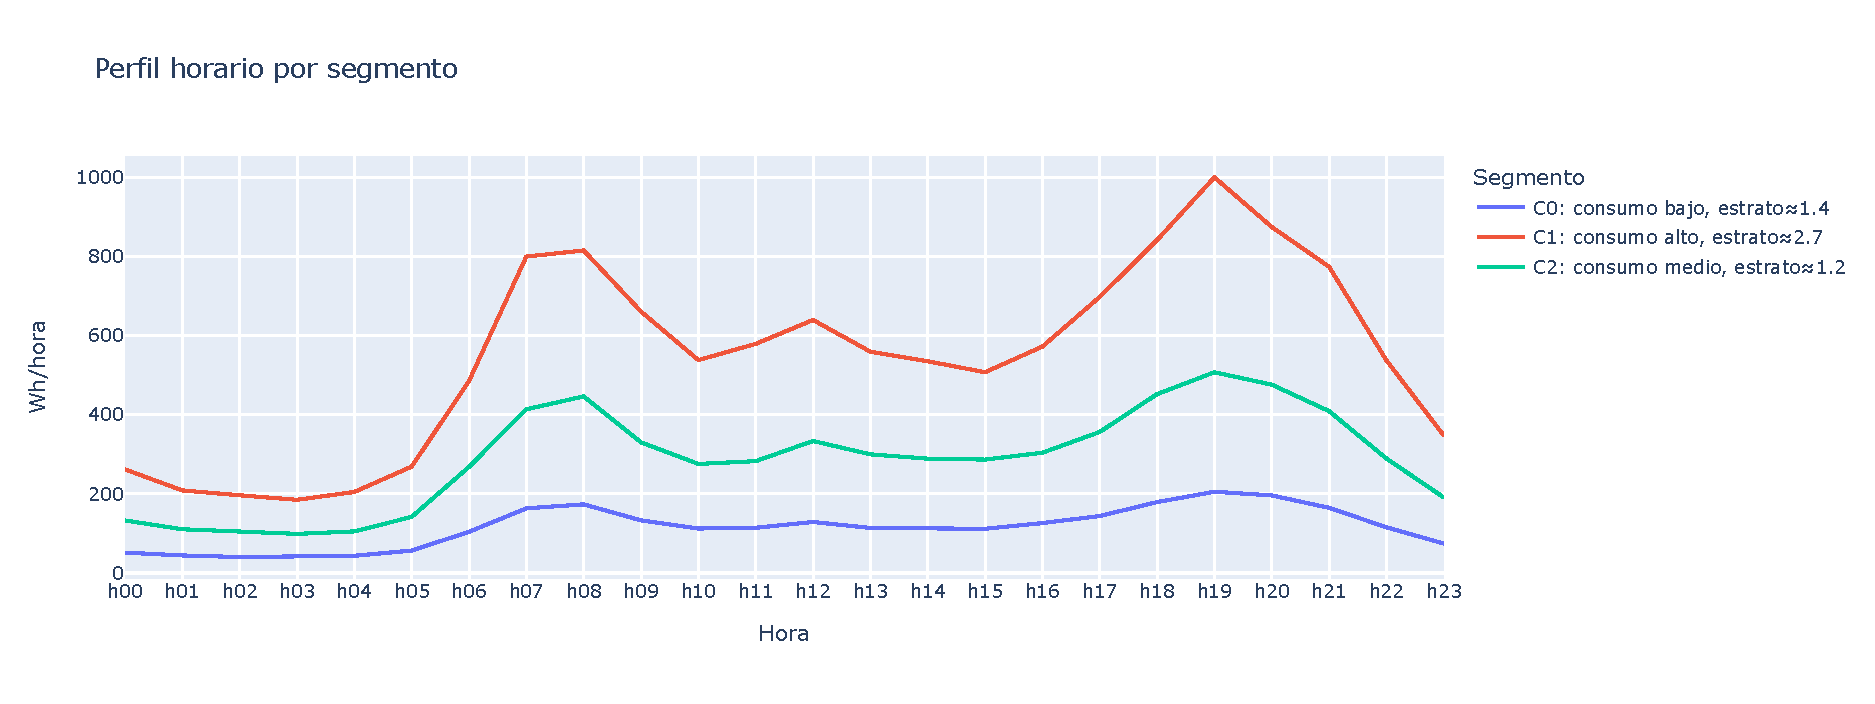
\includegraphics[width=\columnwidth]{figuras_gradio/kmeans_perfil_horario}\par}
{\par\centering\small\textbf{Figura~G.25:} K-means: perfil horario.\par\vspace{0.8em}}
{\par\centering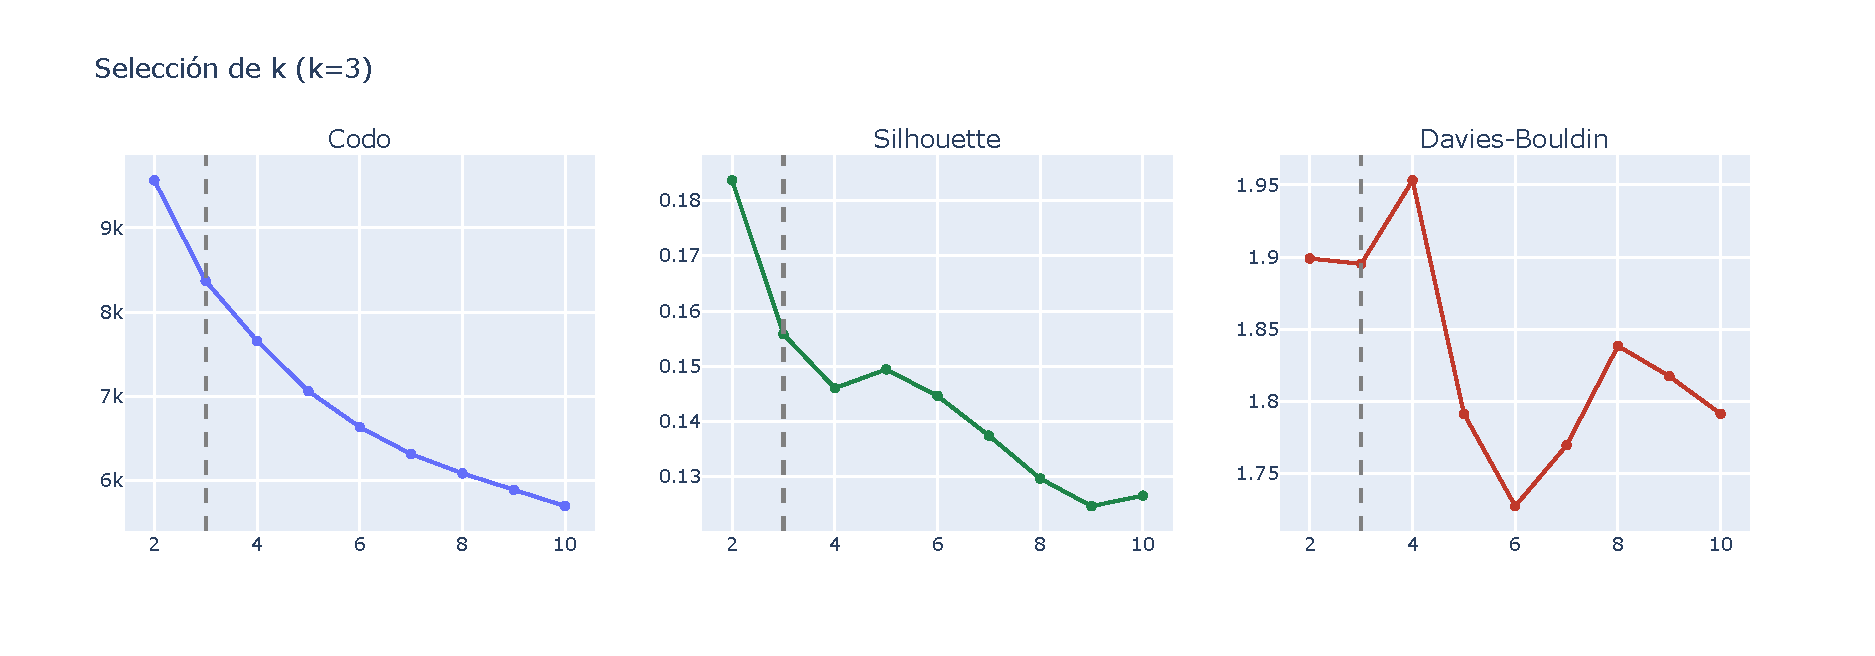
\includegraphics[width=\columnwidth]{figuras_gradio/kmeans_seleccion_k}\par}
{\par\centering\small\textbf{Figura~G.26:} K-means: seleccion k.\par\vspace{0.8em}}
{\par\centering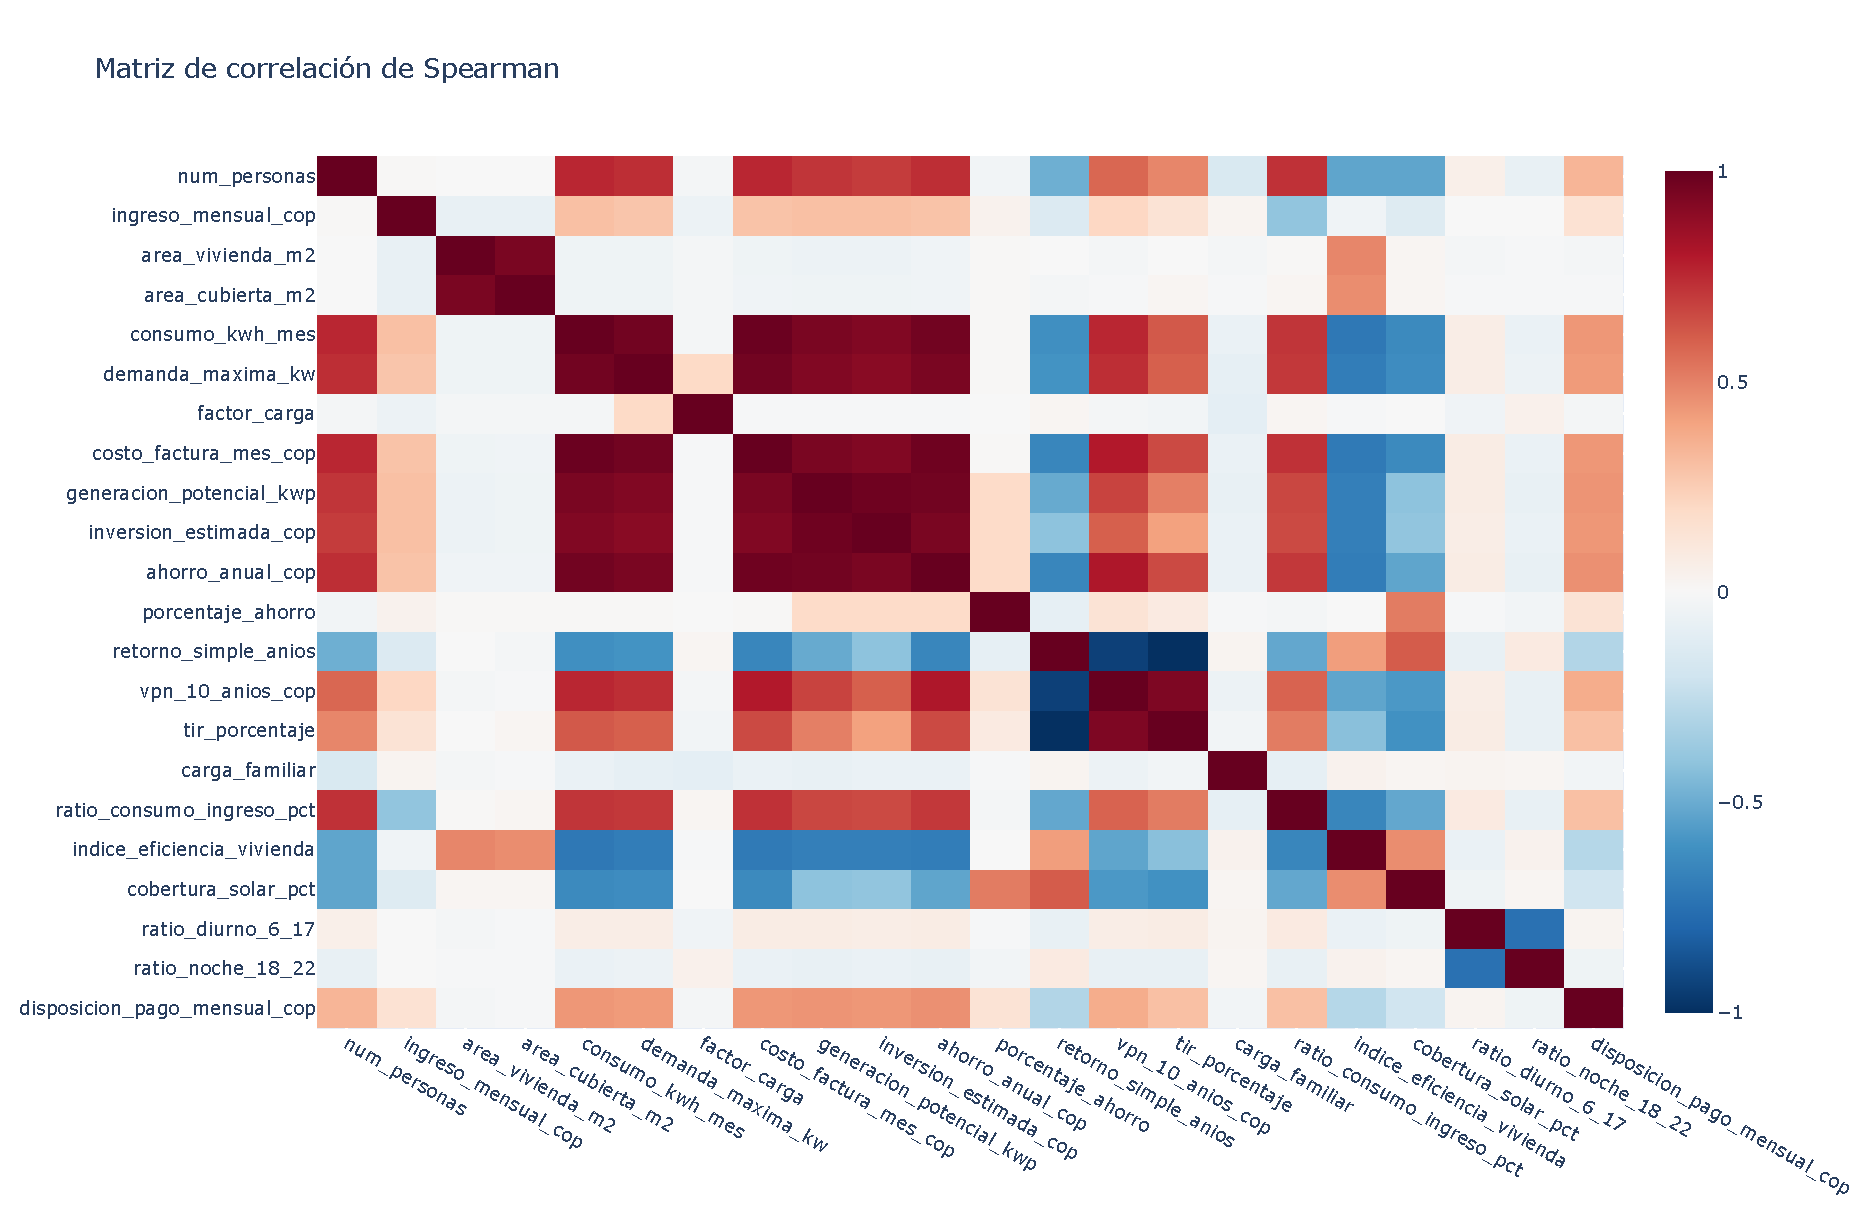
\includegraphics[width=\columnwidth]{figuras_gradio/matriz_correlacion}\par}
{\par\centering\small\textbf{Figura~G.27:} Matriz: correlacion.\par\vspace{0.8em}}
{\par\centering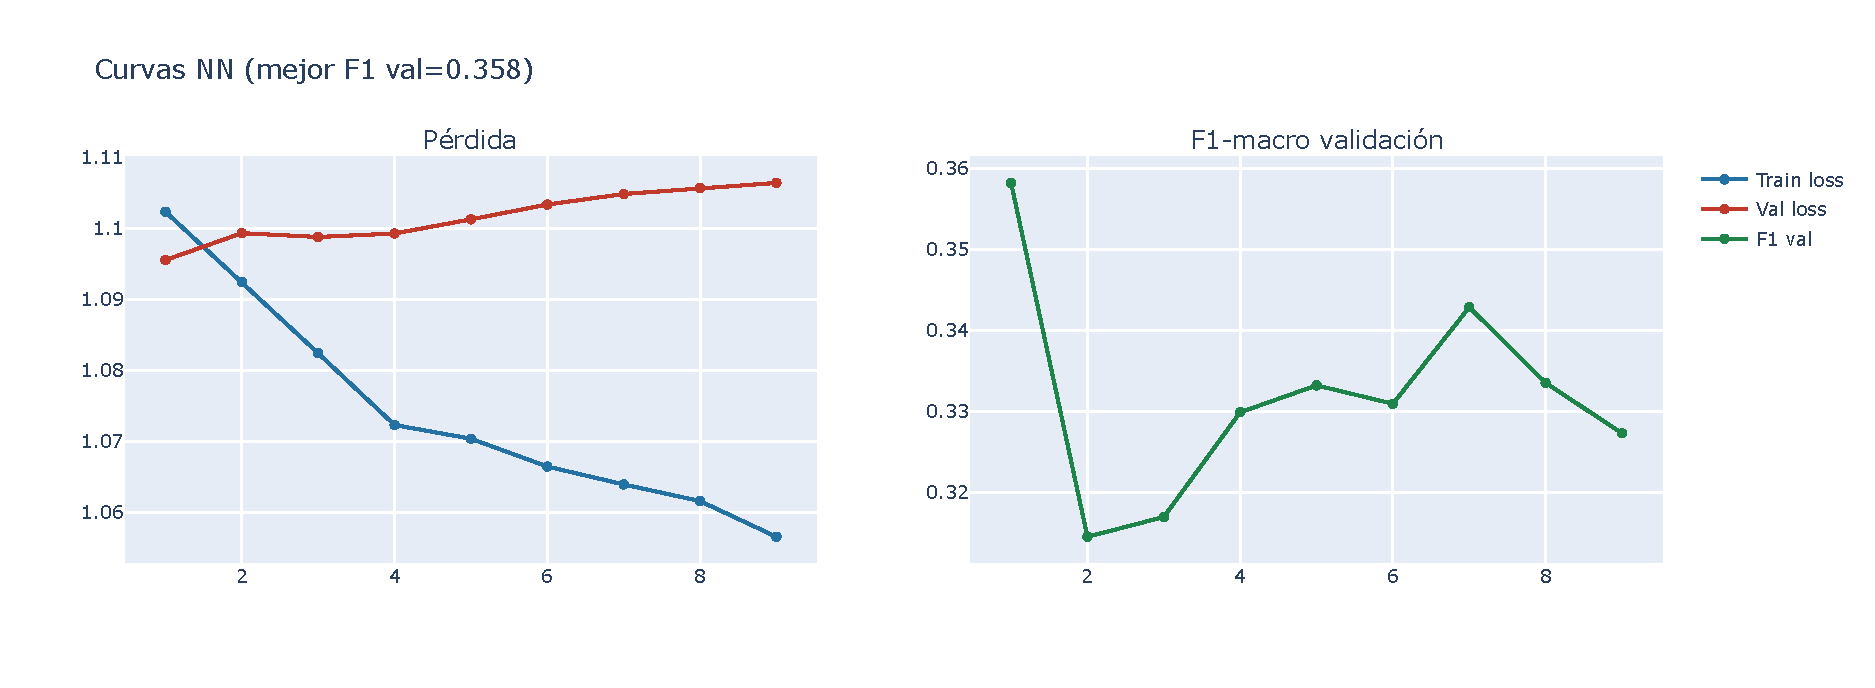
\includegraphics[width=\columnwidth]{figuras_gradio/nn_curvas_entrenamiento}\par}
{\par\centering\small\textbf{Figura~G.28:} Red neuronal: curvas entrenamiento.\par\vspace{0.8em}}
{\par\centering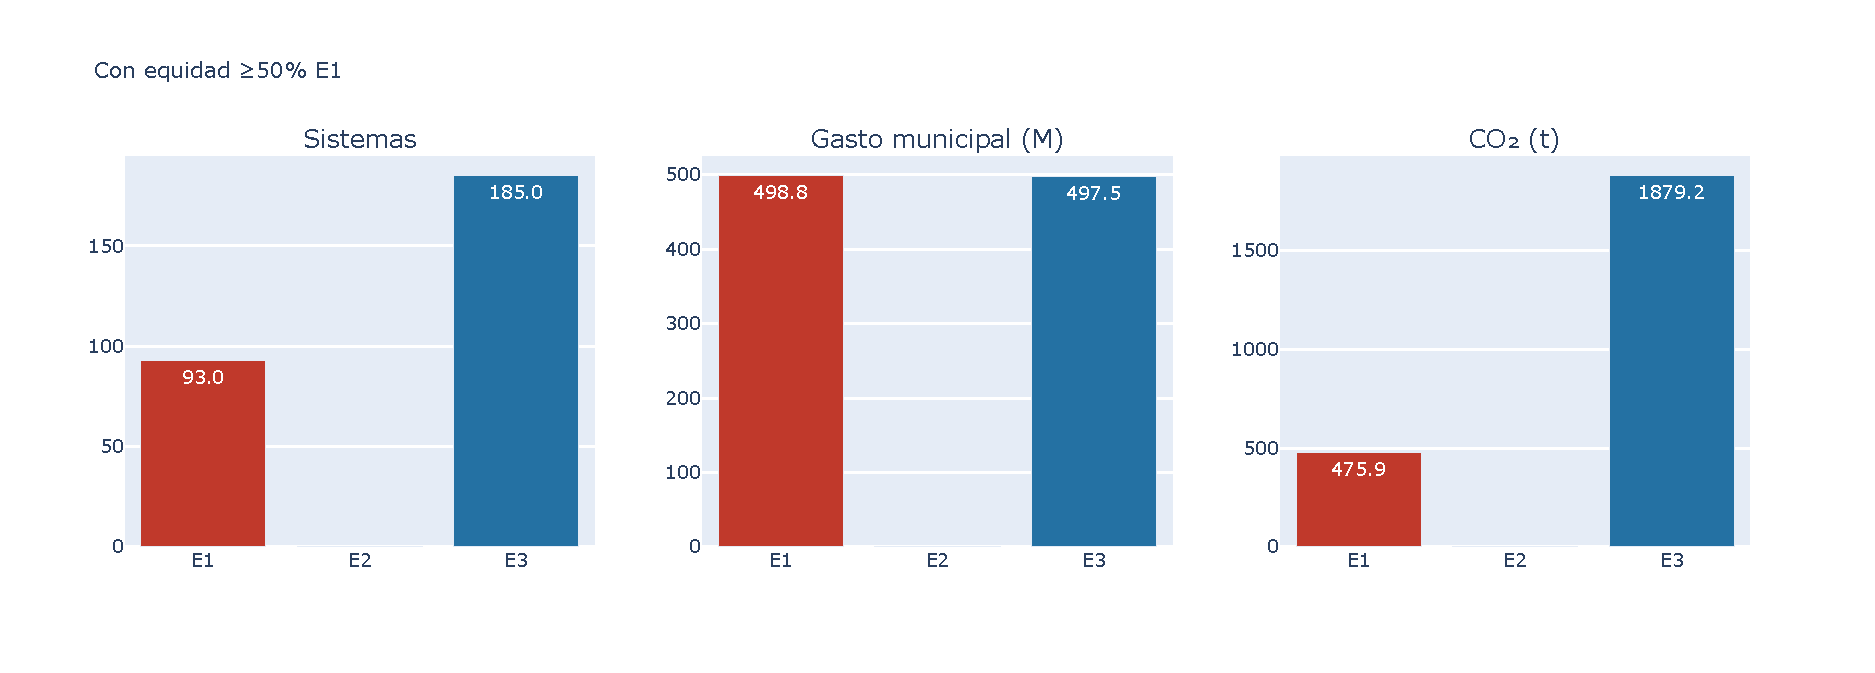
\includegraphics[width=\columnwidth]{figuras_gradio/opt_con_equidad}\par}
{\par\centering\small\textbf{Figura~G.29:} Optimización: con equidad.\par\vspace{0.8em}}
{\par\centering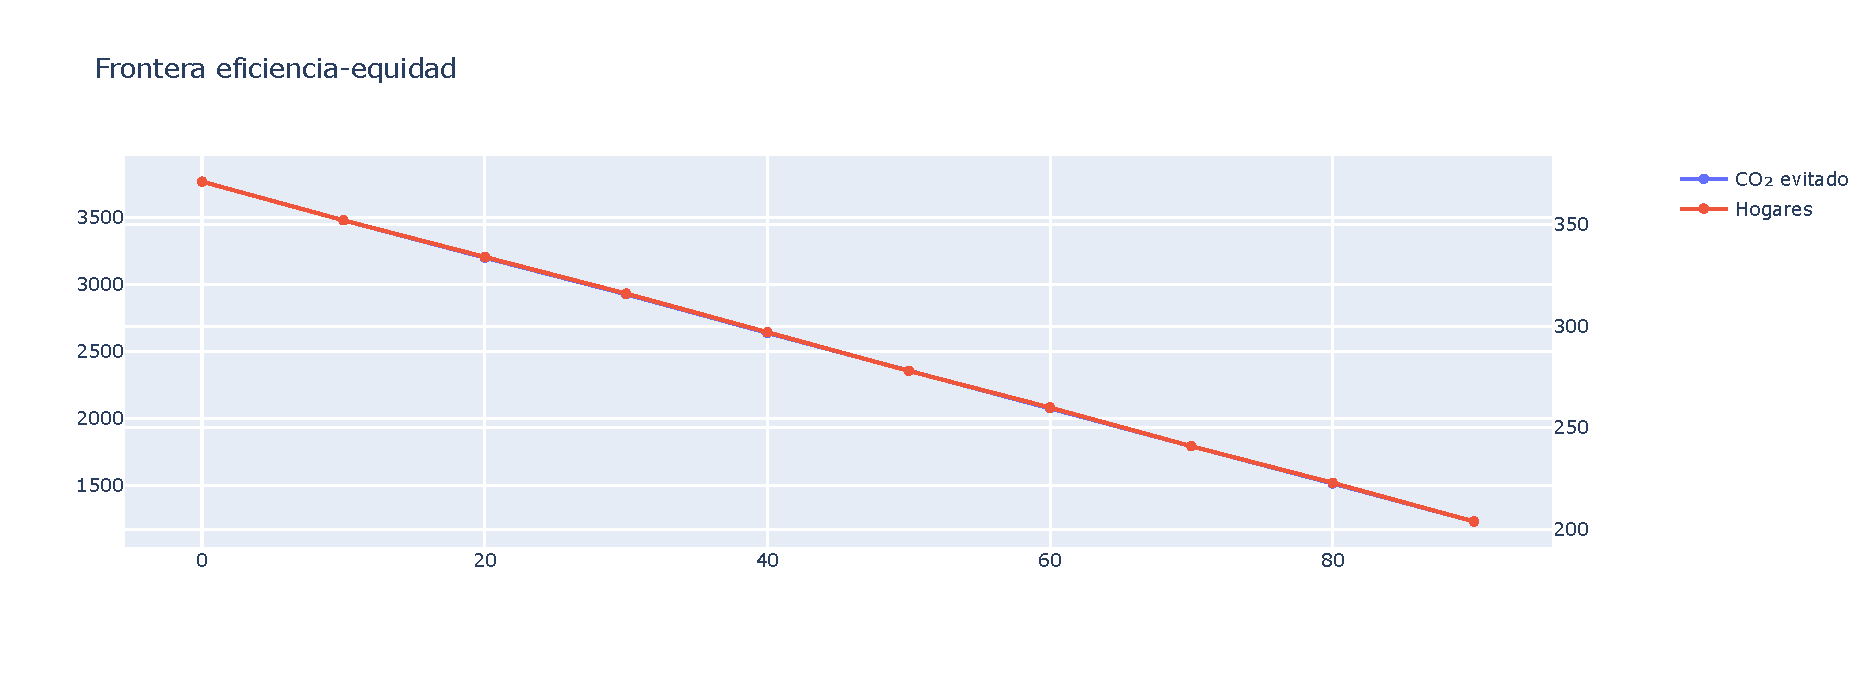
\includegraphics[width=\columnwidth]{figuras_gradio/opt_frontera_equidad}\par}
{\par\centering\small\textbf{Figura~G.30:} Optimización: frontera equidad.\par\vspace{0.8em}}
{\par\centering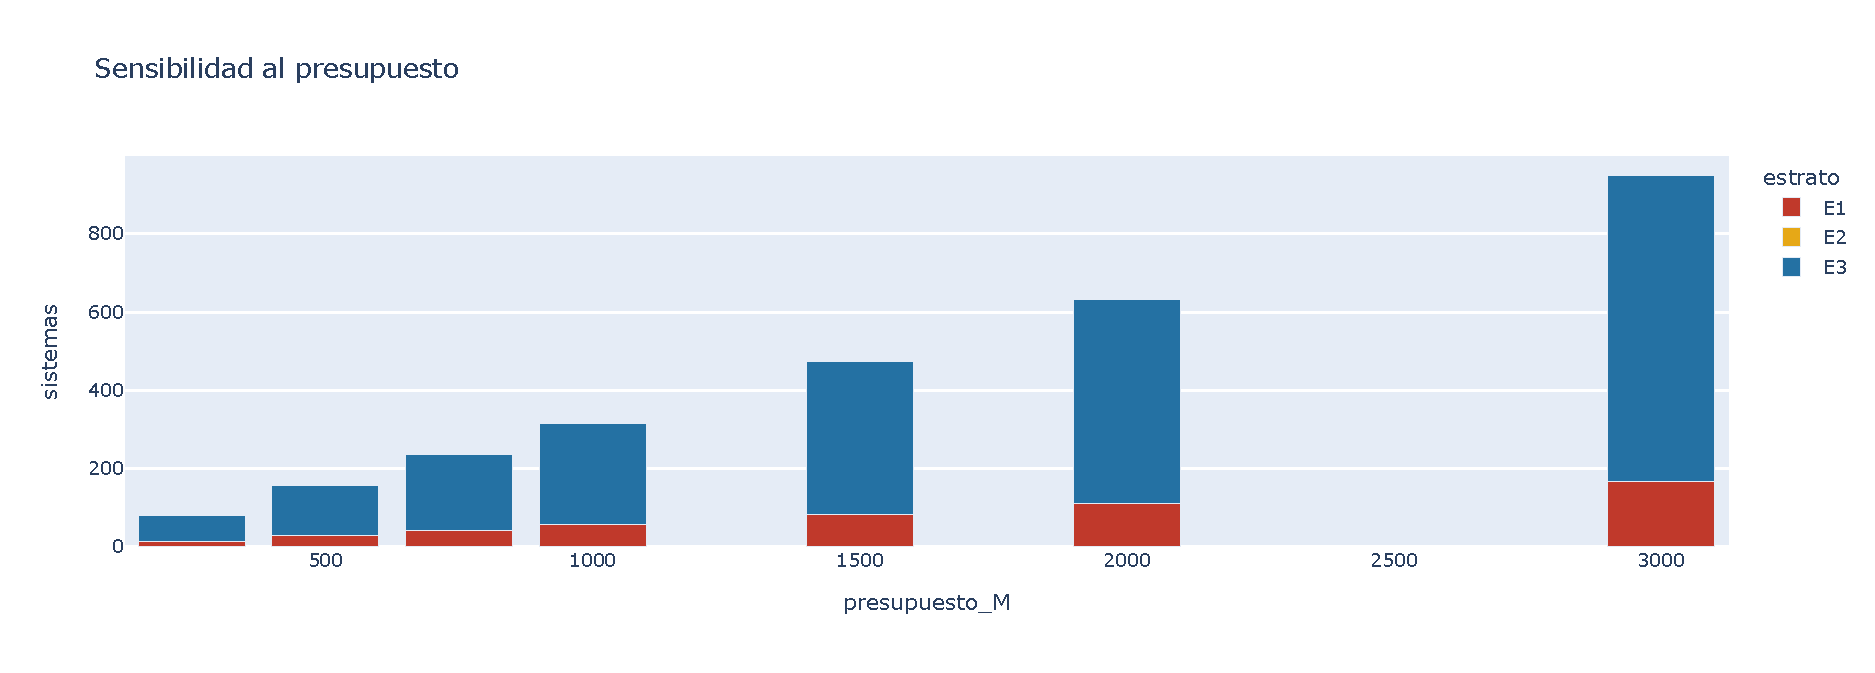
\includegraphics[width=\columnwidth]{figuras_gradio/opt_sensibilidad_presupuesto}\par}
{\par\centering\small\textbf{Figura~G.31:} Optimización: sensibilidad presupuesto.\par\vspace{0.8em}}
{\par\centering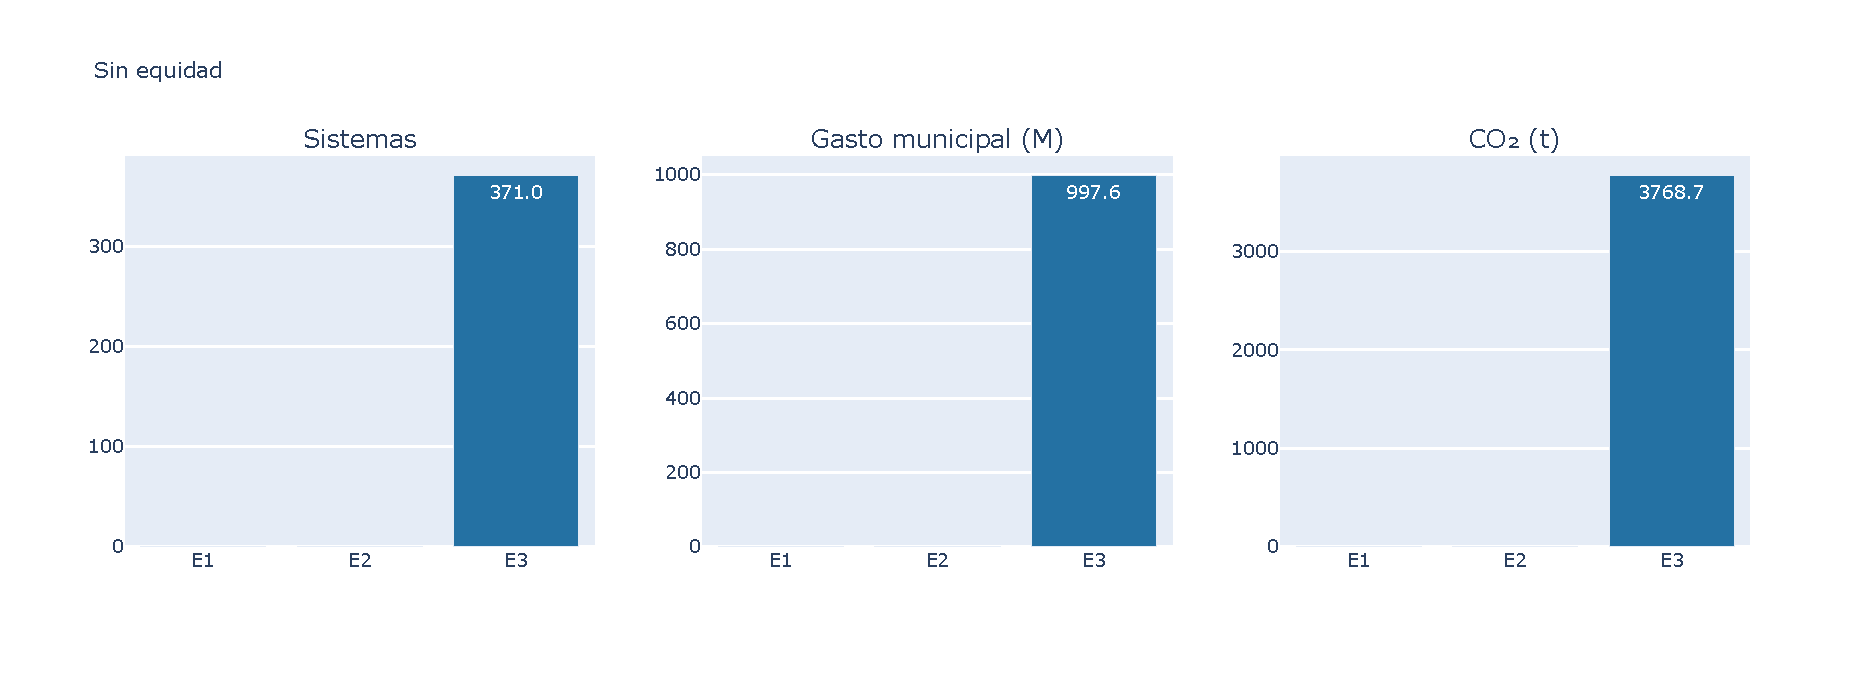
\includegraphics[width=\columnwidth]{figuras_gradio/opt_sin_equidad}\par}
{\par\centering\small\textbf{Figura~G.32:} Optimización: sin equidad.\par\vspace{0.8em}}
{\par\centering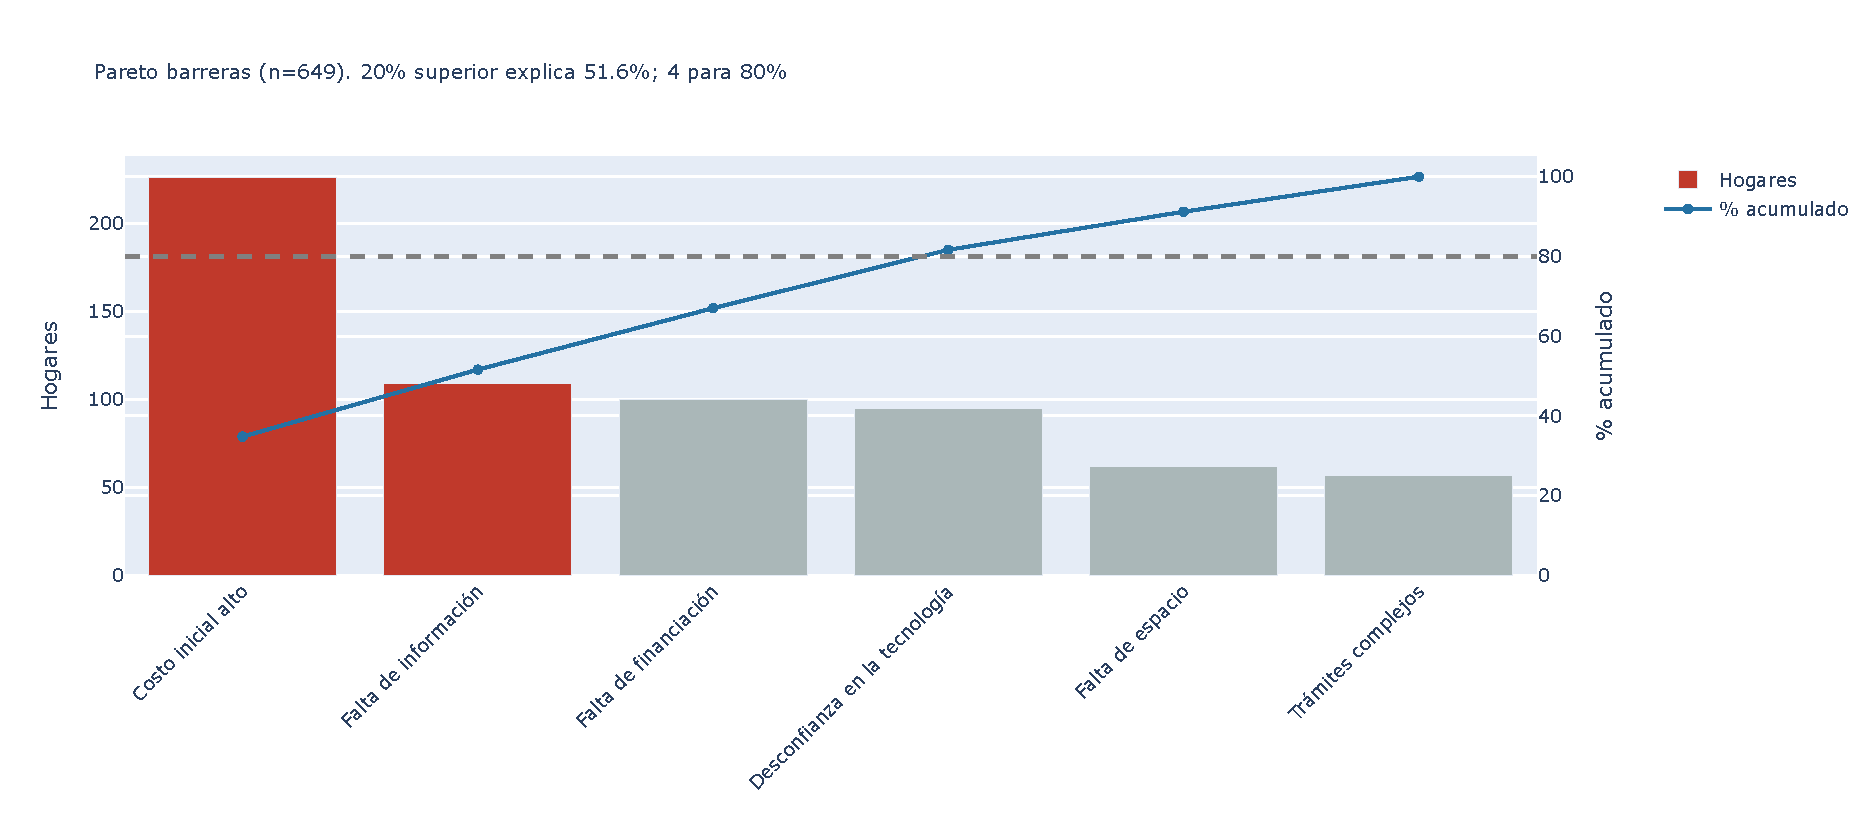
\includegraphics[width=\columnwidth]{figuras_gradio/pareto_barreras}\par}
{\par\centering\small\textbf{Figura~G.33:} Pareto: barreras.\par\vspace{0.8em}}
{\par\centering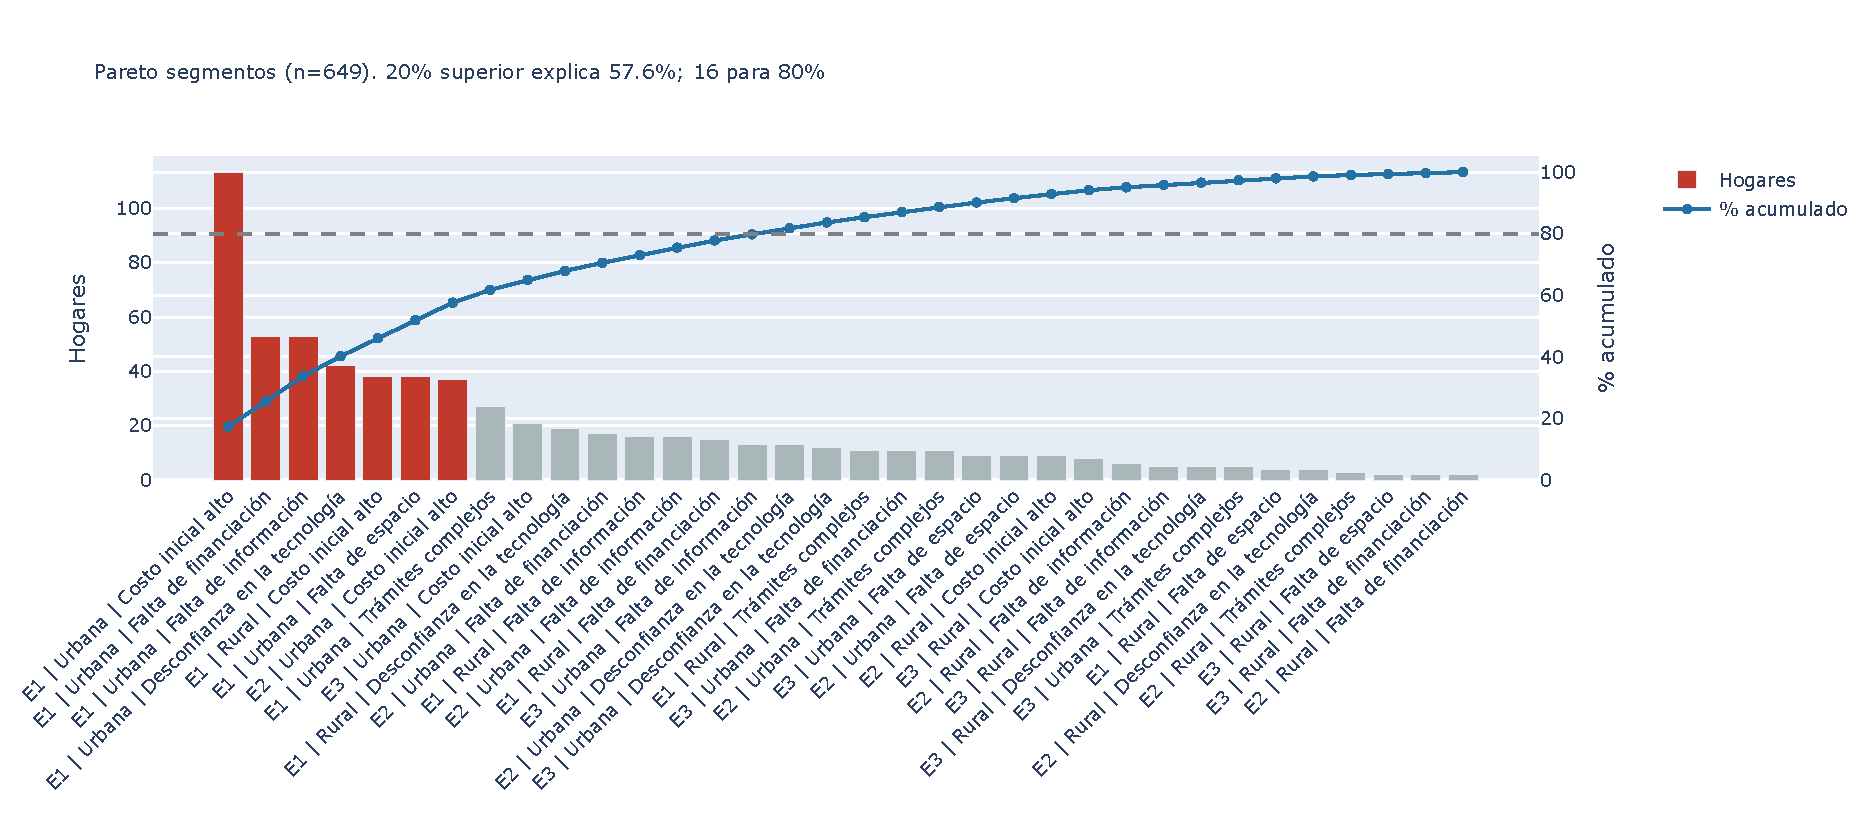
\includegraphics[width=\columnwidth]{figuras_gradio/pareto_segmentos}\par}
{\par\centering\small\textbf{Figura~G.34:} Pareto: segmentos.\par\vspace{0.8em}}
{\par\centering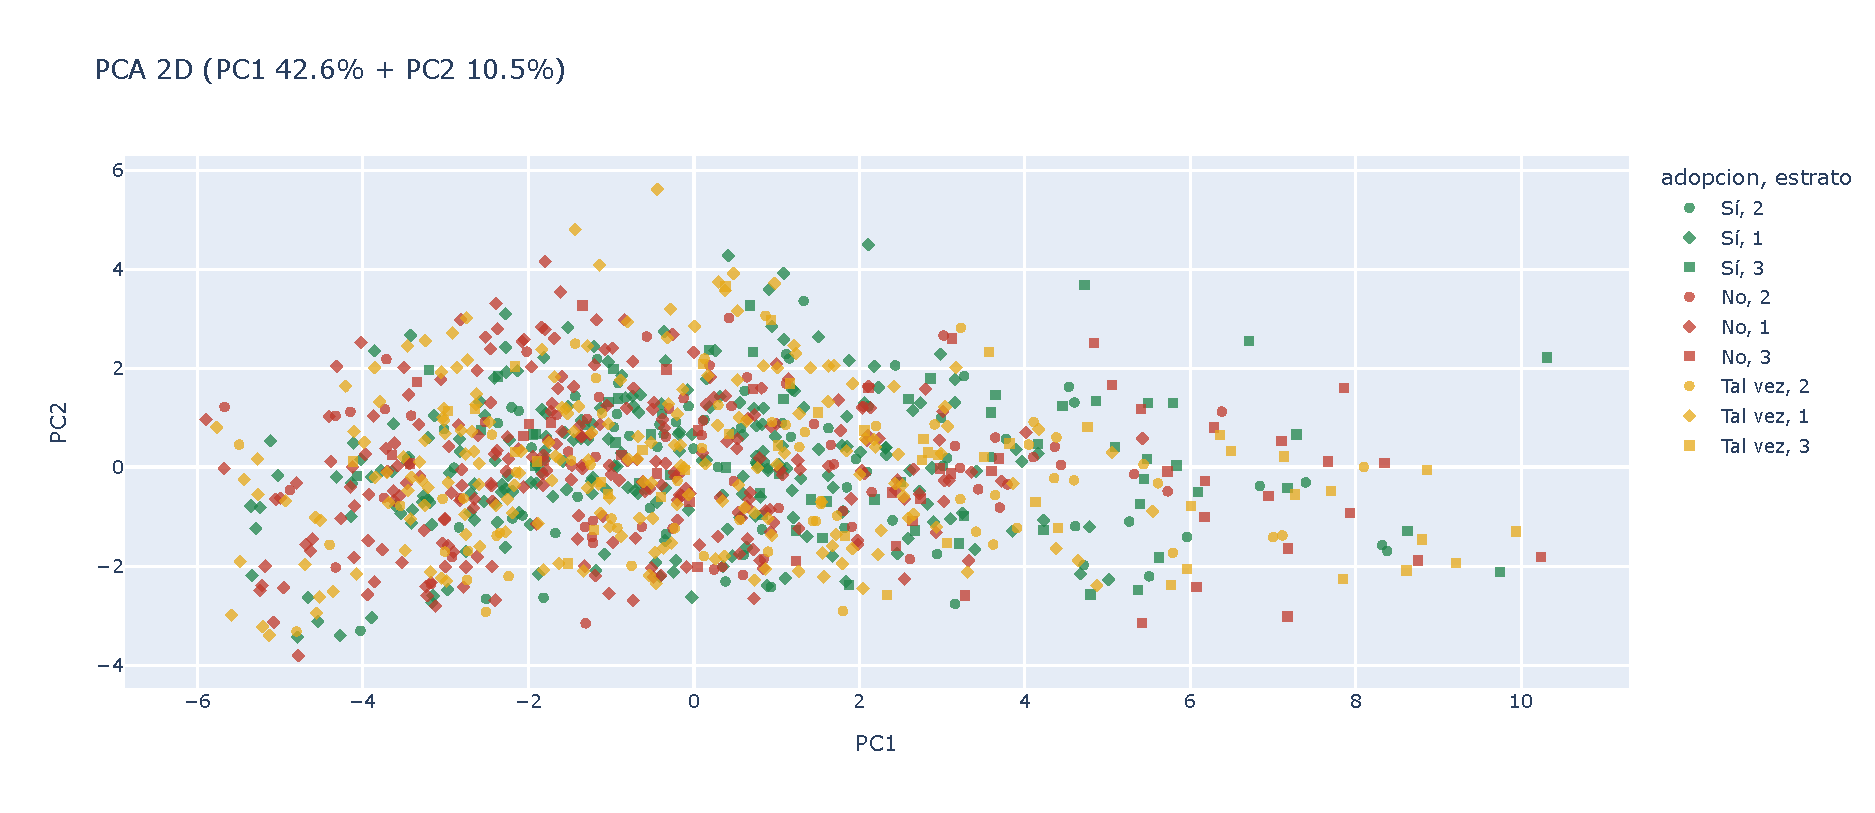
\includegraphics[width=\columnwidth]{figuras_gradio/pca_2d}\par}
{\par\centering\small\textbf{Figura~G.35:} Pca: 2d.\par\vspace{0.8em}}
{\par\centering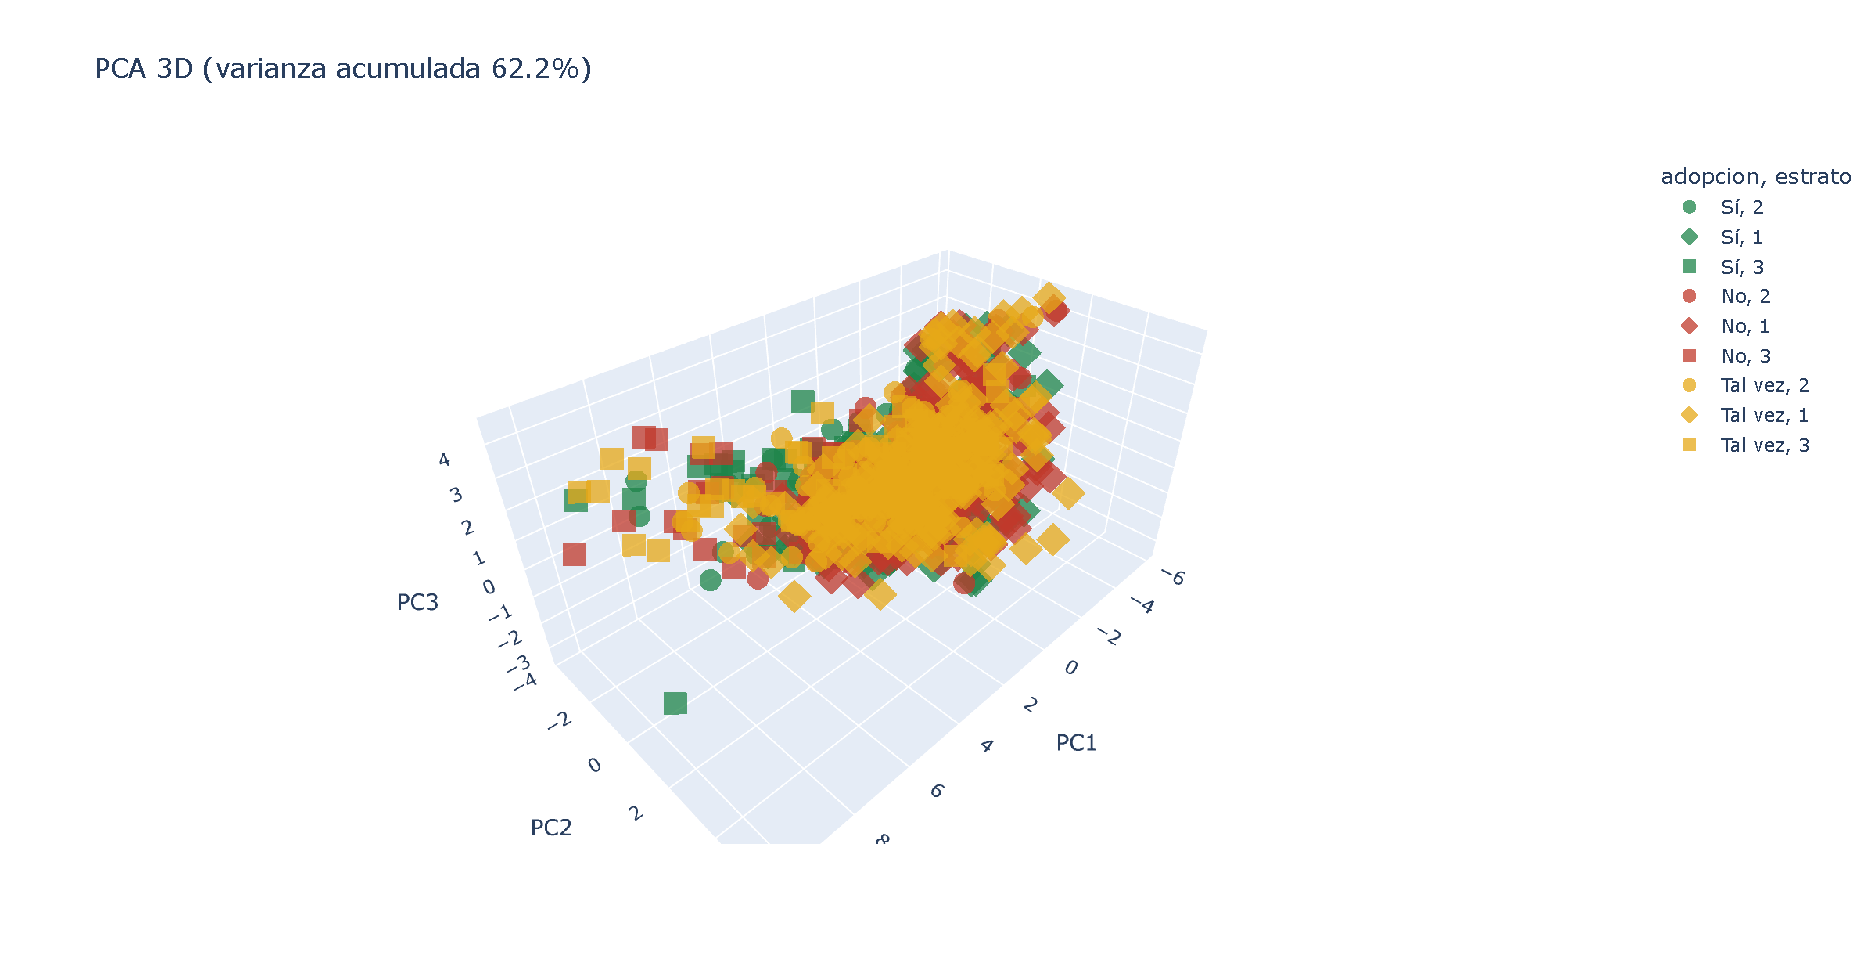
\includegraphics[width=\columnwidth]{figuras_gradio/pca_3d}\par}
{\par\centering\small\textbf{Figura~G.36:} Pca: 3d.\par\vspace{0.8em}}
{\par\centering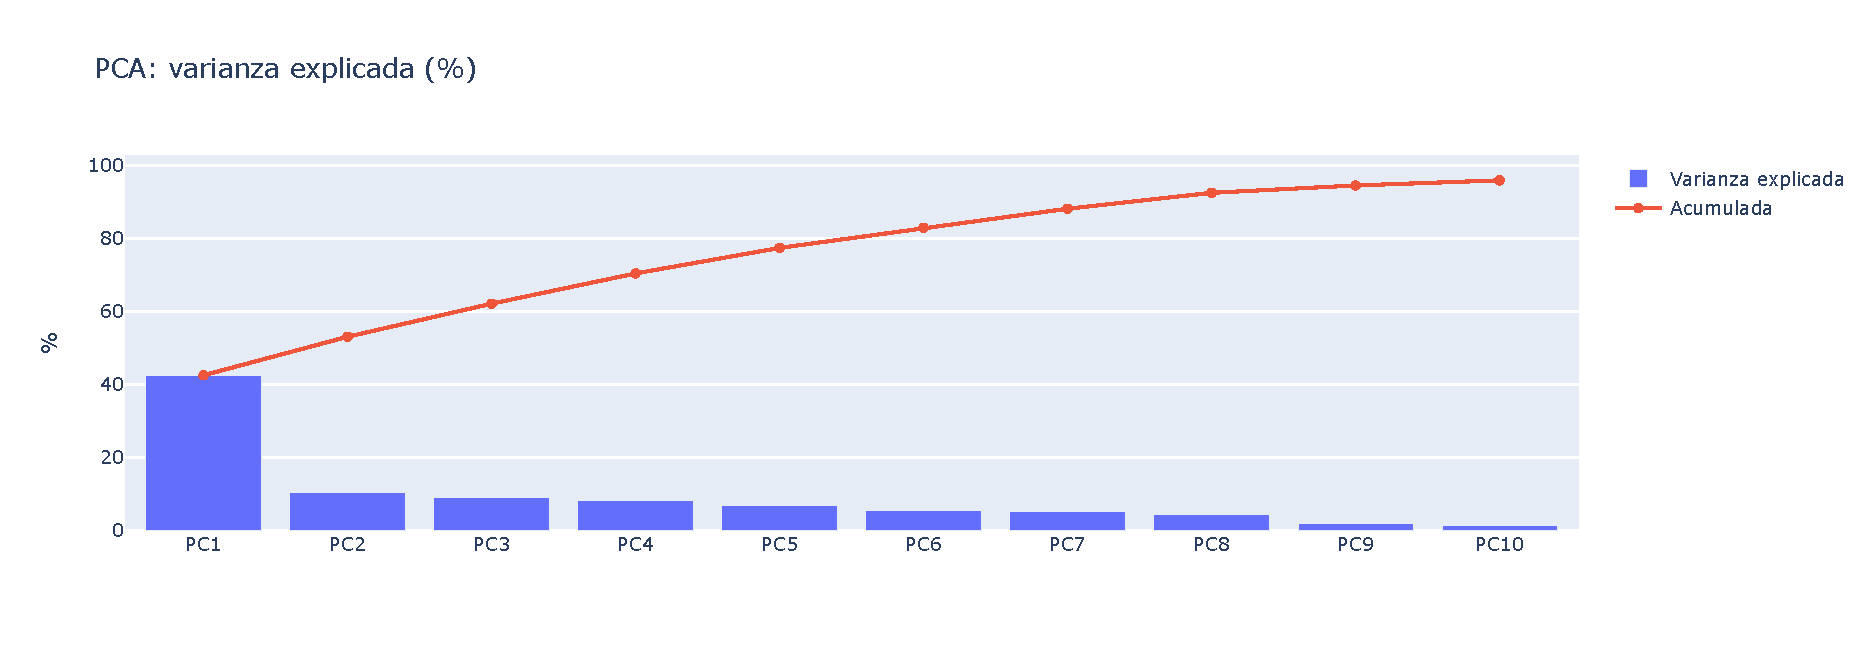
\includegraphics[width=\columnwidth]{figuras_gradio/pca_varianza}\par}
{\par\centering\small\textbf{Figura~G.37:} Pca: varianza.\par\vspace{0.8em}}
{\par\centering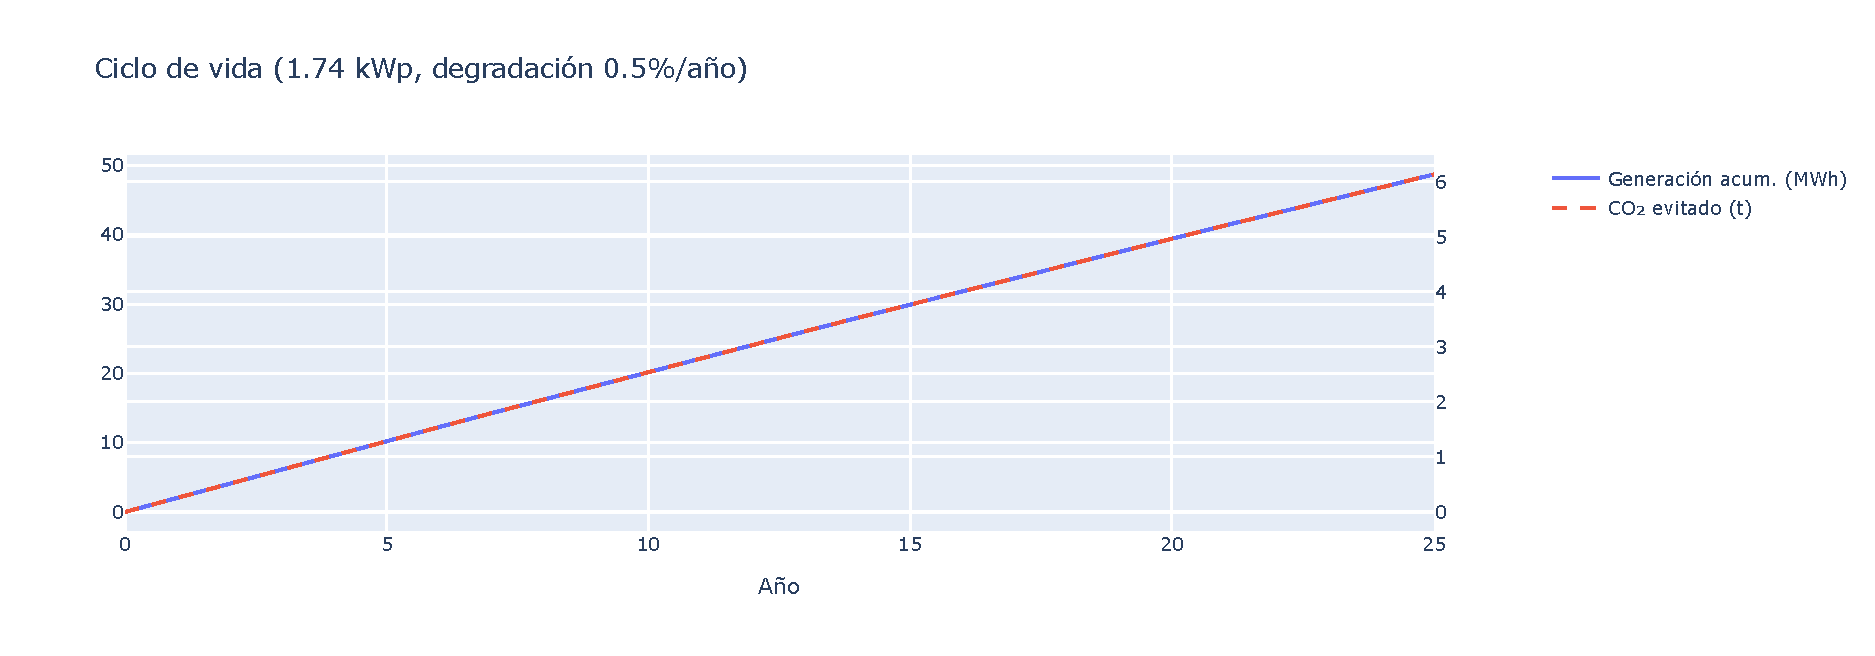
\includegraphics[width=\columnwidth]{figuras_gradio/raee_ciclo_vida}\par}
{\par\centering\small\textbf{Figura~G.38:} Raee: ciclo vida.\par\vspace{0.8em}}
{\par\centering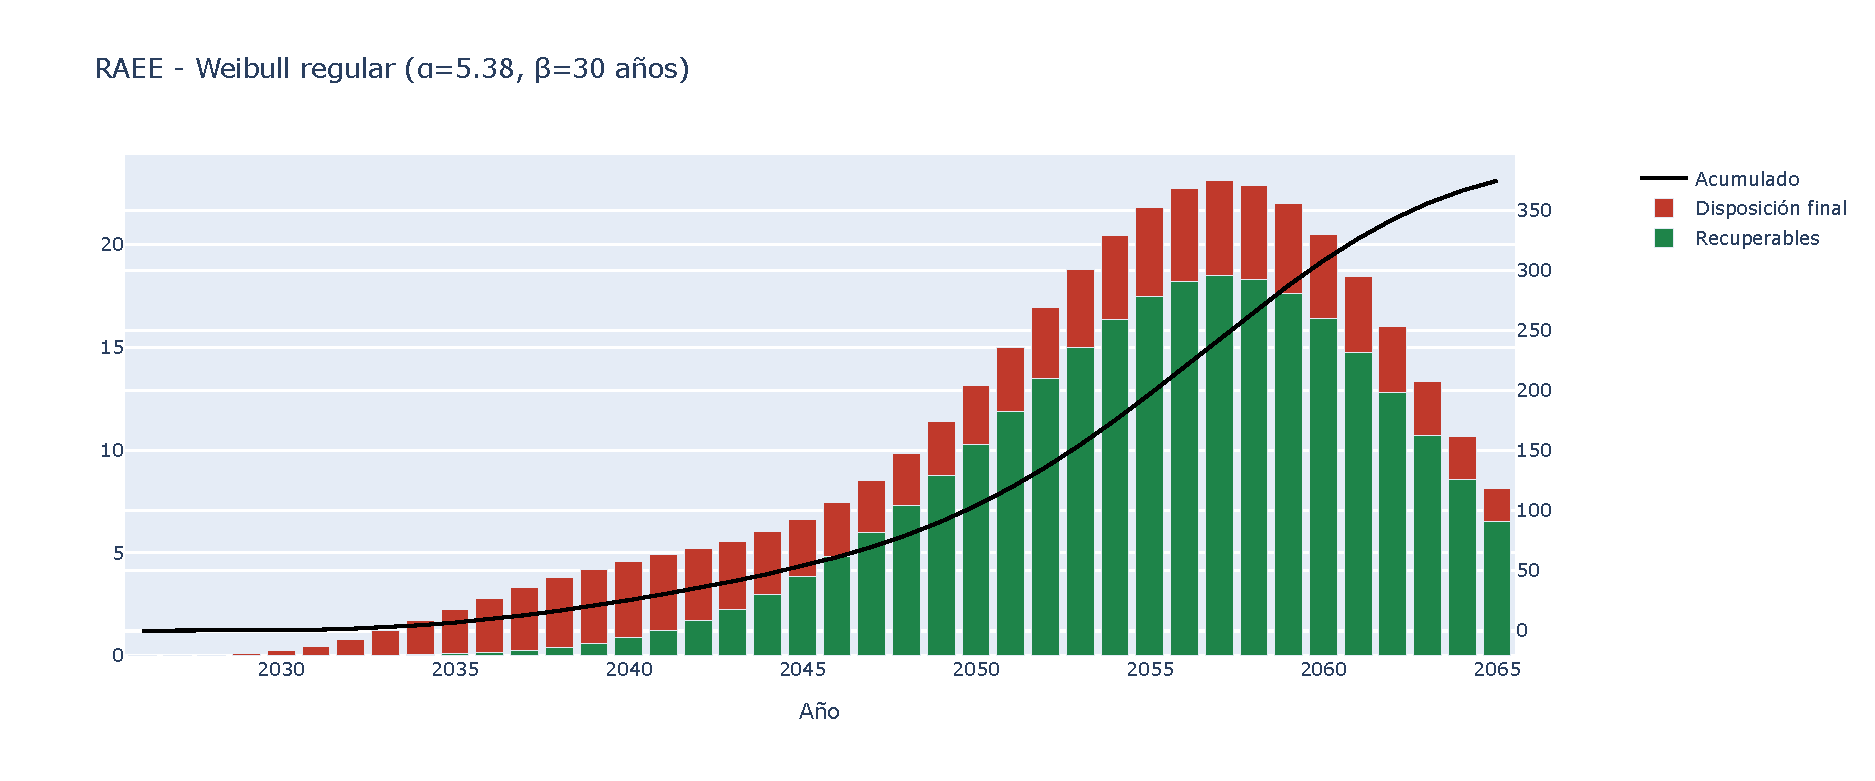
\includegraphics[width=\columnwidth]{figuras_gradio/raee_escenario_1}\par}
{\par\centering\small\textbf{Figura~G.39:} Raee: escenario 1.\par\vspace{0.8em}}
{\par\centering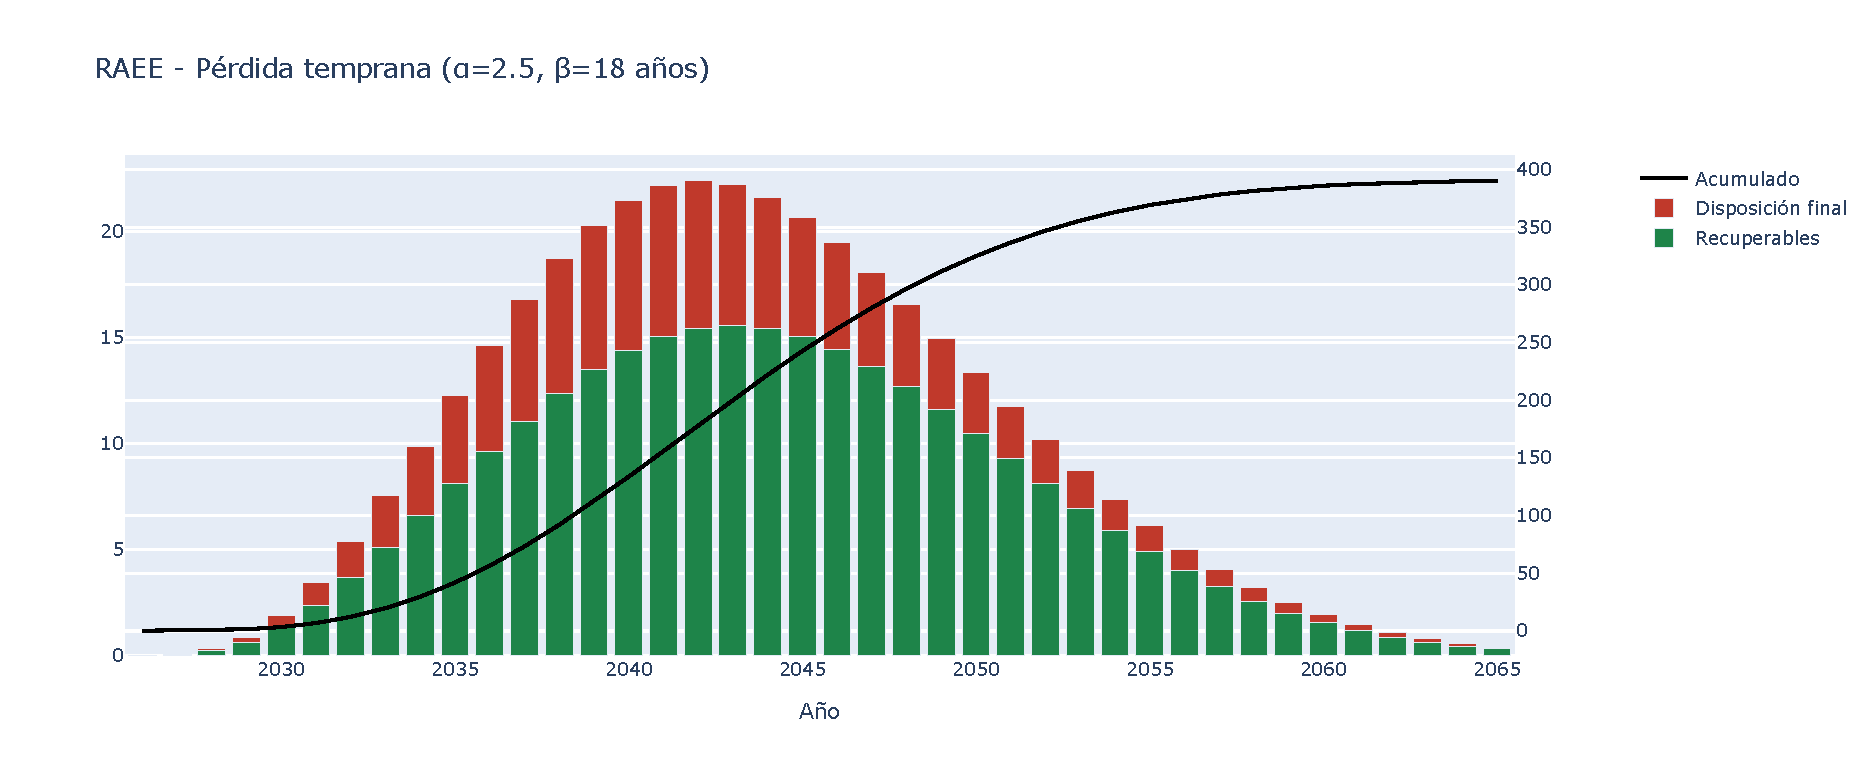
\includegraphics[width=\columnwidth]{figuras_gradio/raee_escenario_2}\par}
{\par\centering\small\textbf{Figura~G.40:} Raee: escenario 2.\par\vspace{0.8em}}
{\par\centering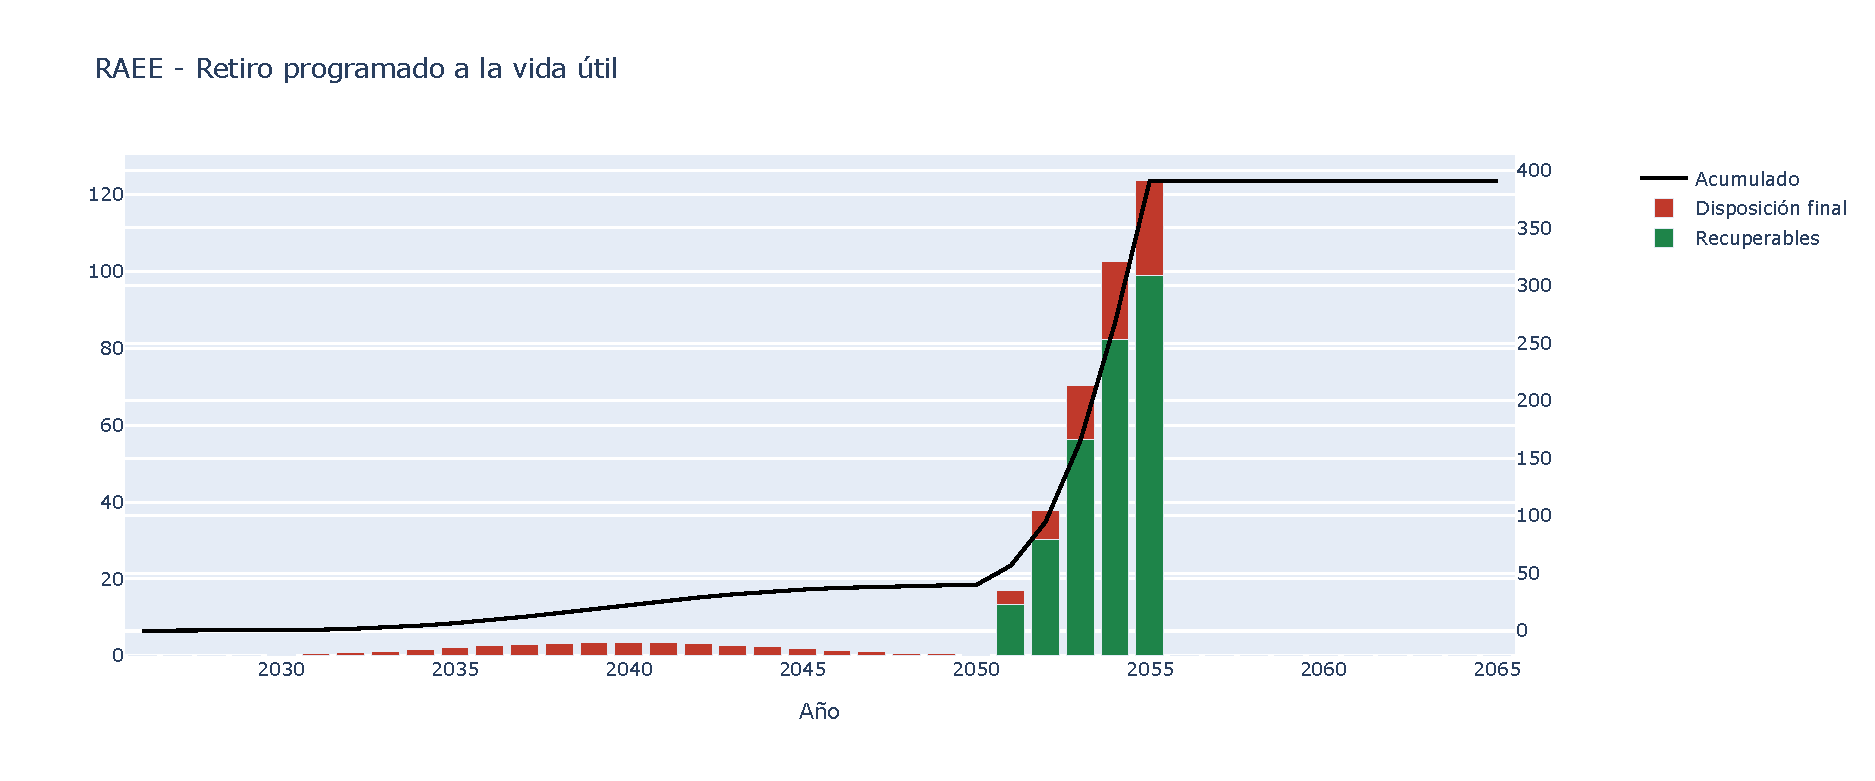
\includegraphics[width=\columnwidth]{figuras_gradio/raee_escenario_3}\par}
{\par\centering\small\textbf{Figura~G.41:} Raee: escenario 3.\par\vspace{0.8em}}
{\par\centering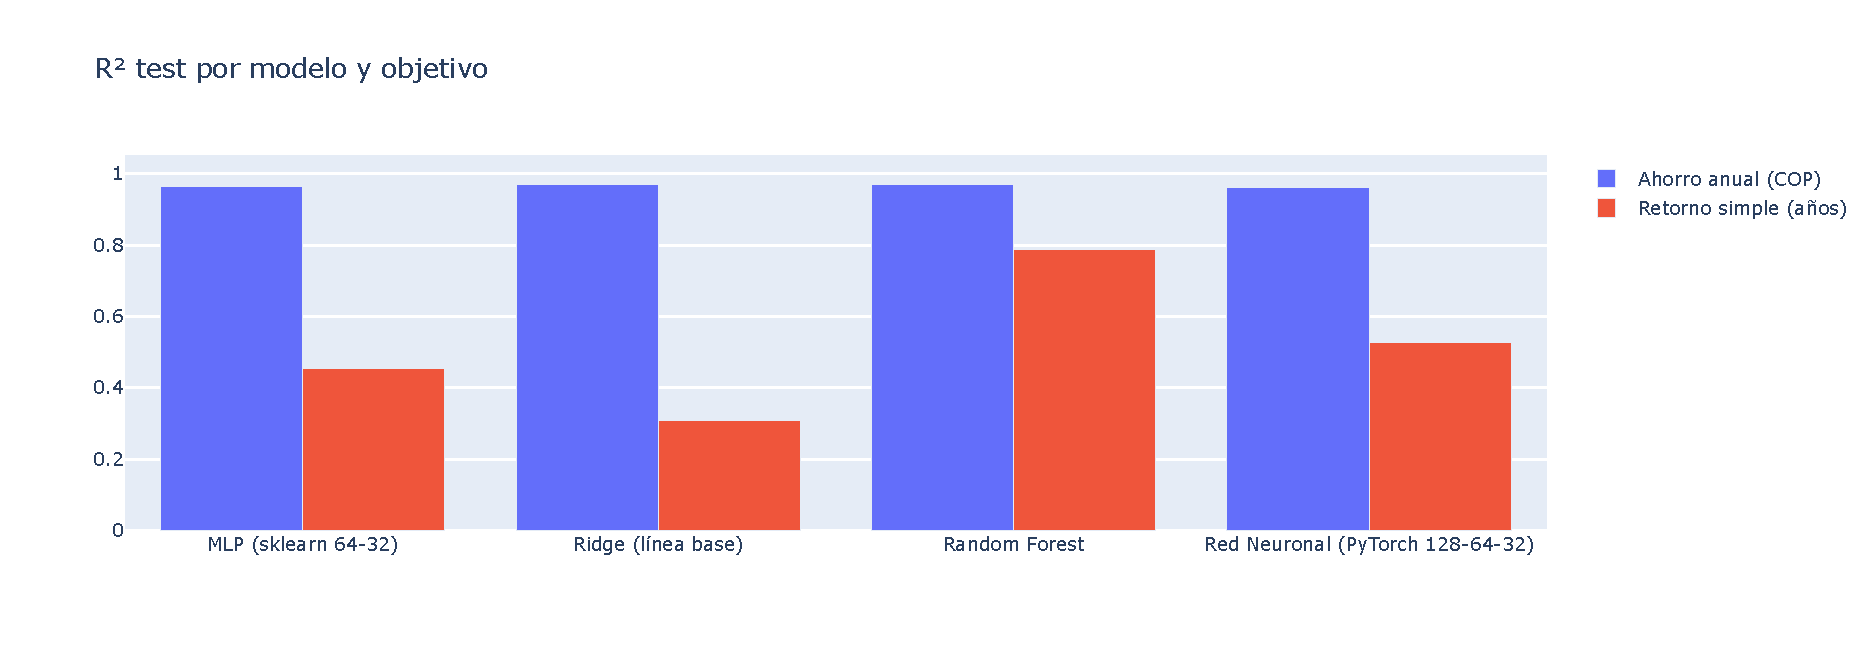
\includegraphics[width=\columnwidth]{figuras_gradio/reg_comparacion}\par}
{\par\centering\small\textbf{Figura~G.42:} Regresión: comparacion.\par\vspace{0.8em}}
{\par\centering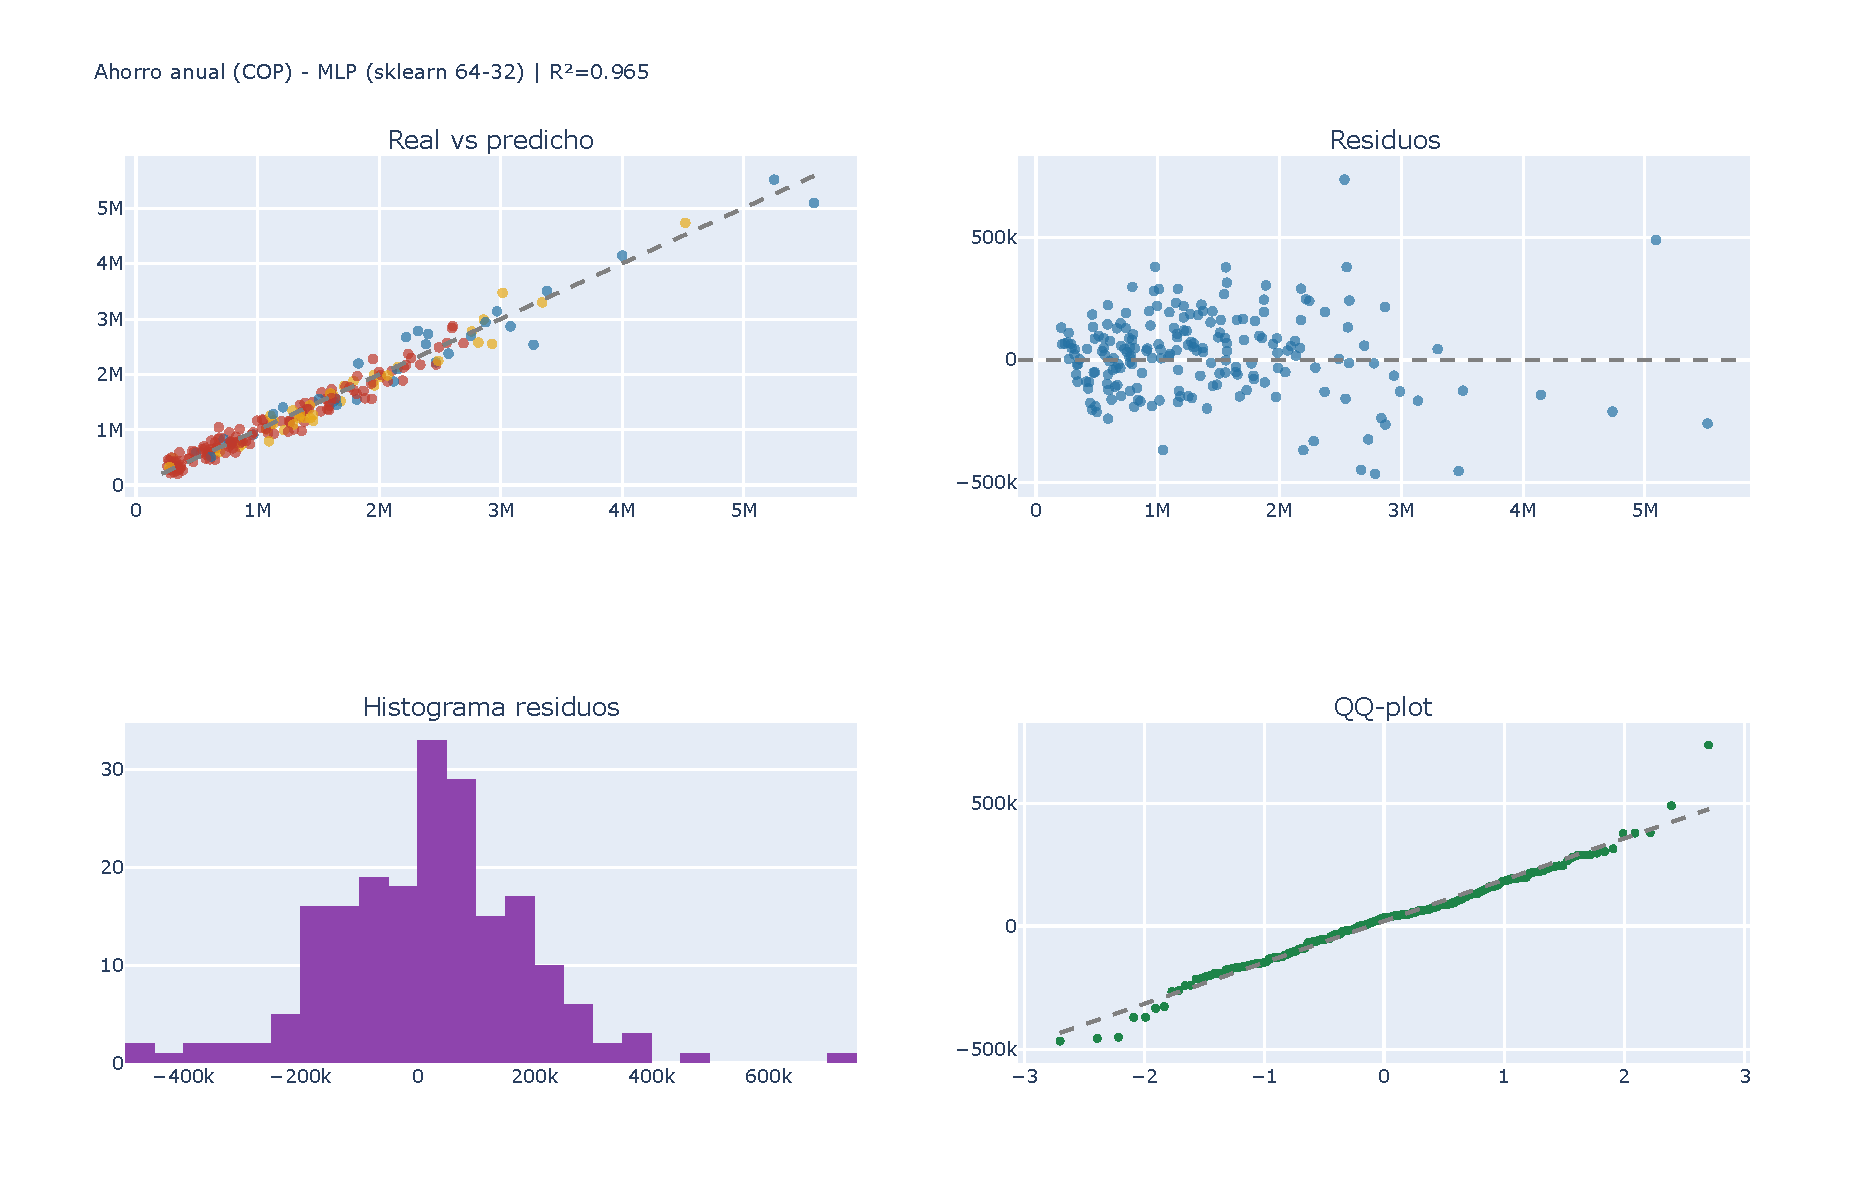
\includegraphics[width=\columnwidth]{figuras_gradio/reg_diagnostico_ahorro_anual_cop}\par}
{\par\centering\small\textbf{Figura~G.43:} Regresión: diagnostico ahorro anual cop.\par\vspace{0.8em}}
{\par\centering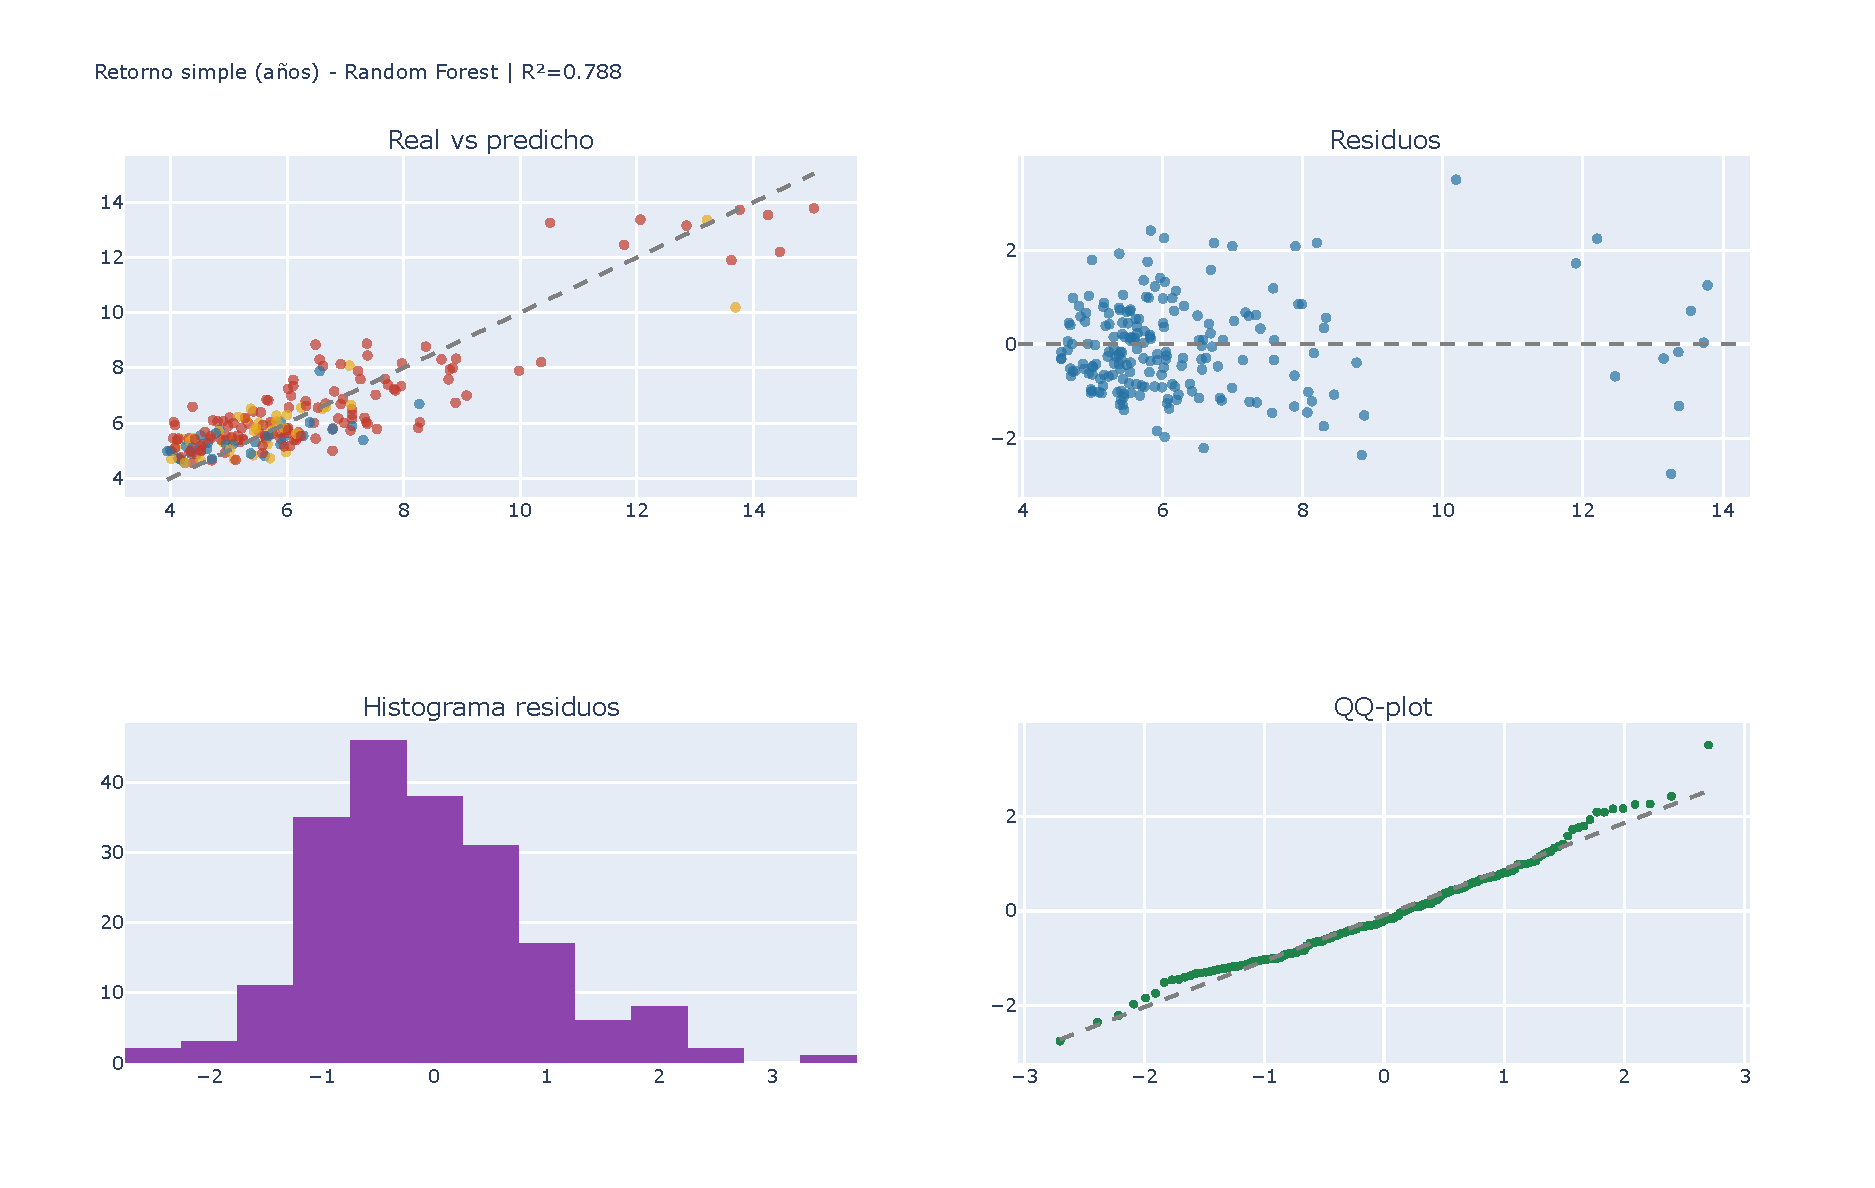
\includegraphics[width=\columnwidth]{figuras_gradio/reg_diagnostico_retorno_simple_anios}\par}
{\par\centering\small\textbf{Figura~G.44:} Regresión: diagnostico retorno simple anios.\par\vspace{0.8em}}
{\par\centering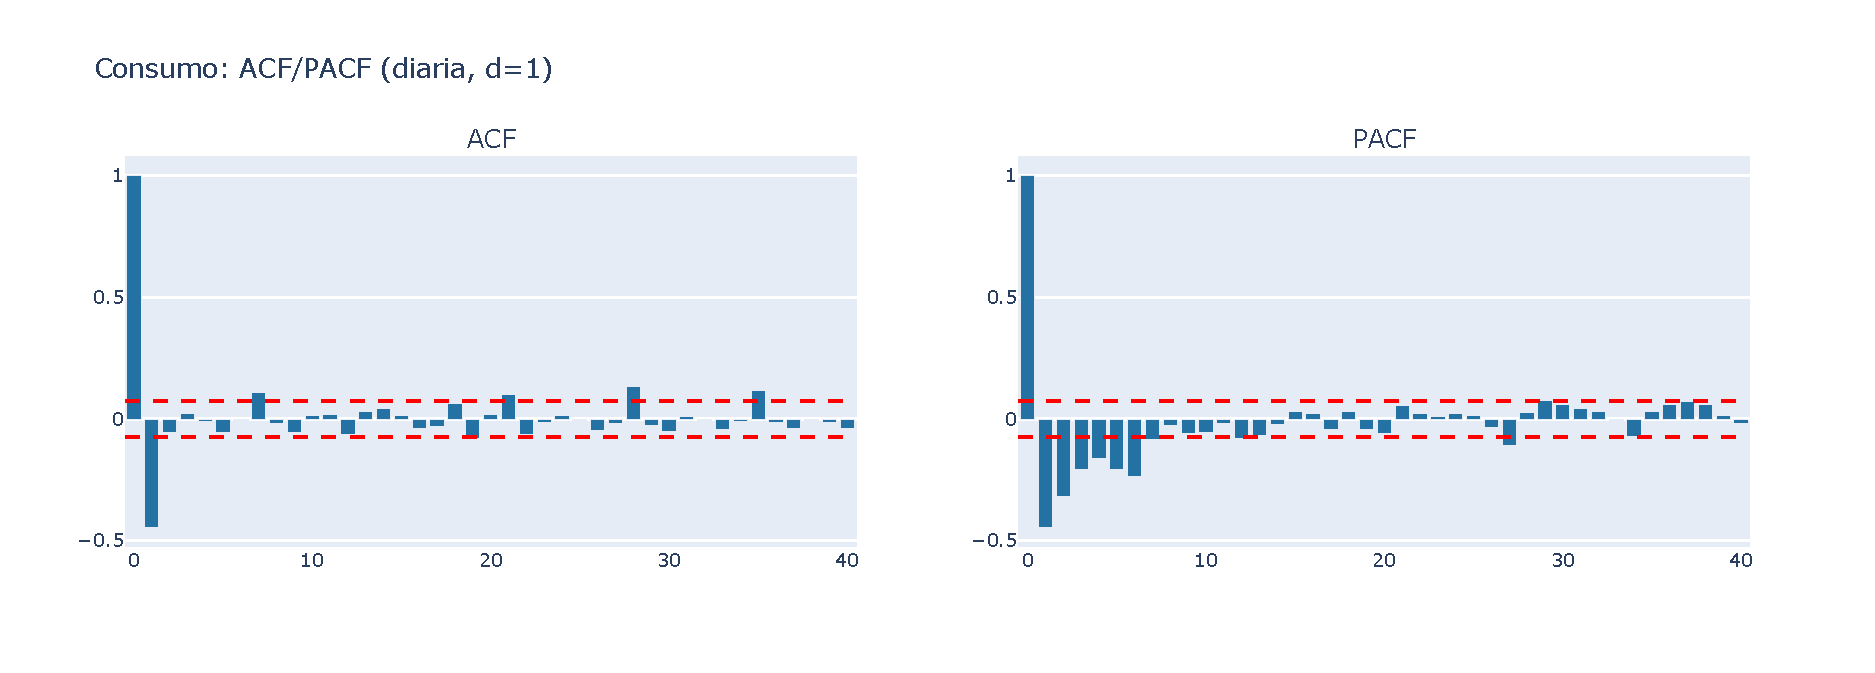
\includegraphics[width=\columnwidth]{figuras_gradio/ts_acf_pacf_consumo}\par}
{\par\centering\small\textbf{Figura~G.45:} Series temporales: acf pacf consumo.\par\vspace{0.8em}}
{\par\centering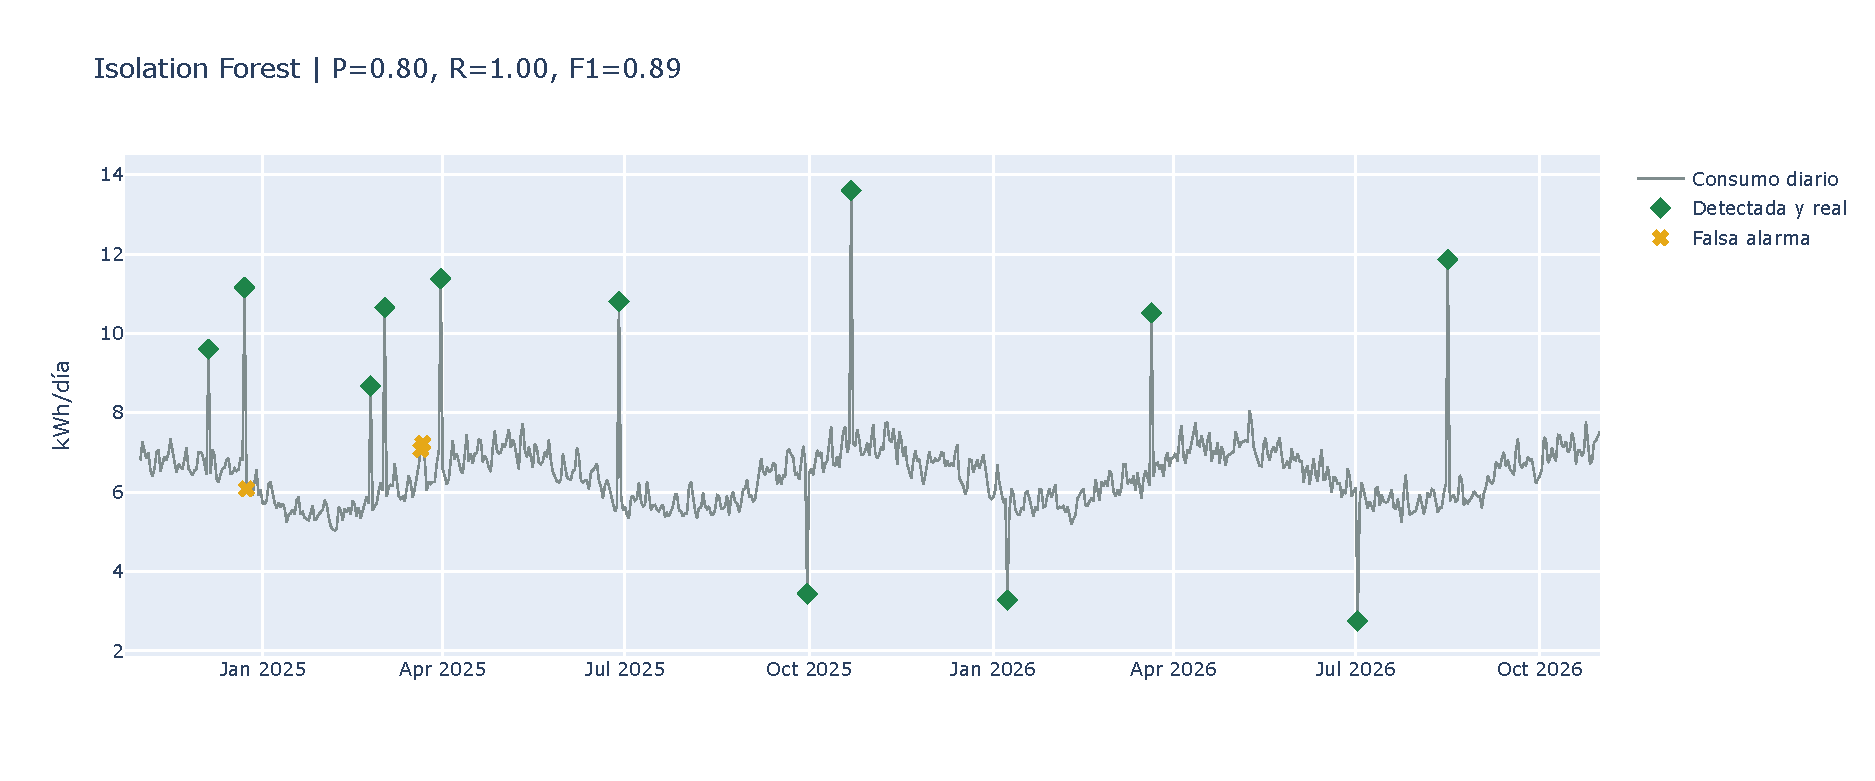
\includegraphics[width=\columnwidth]{figuras_gradio/ts_anomalias}\par}
{\par\centering\small\textbf{Figura~G.46:} Series temporales: anomalias.\par\vspace{0.8em}}
{\par\centering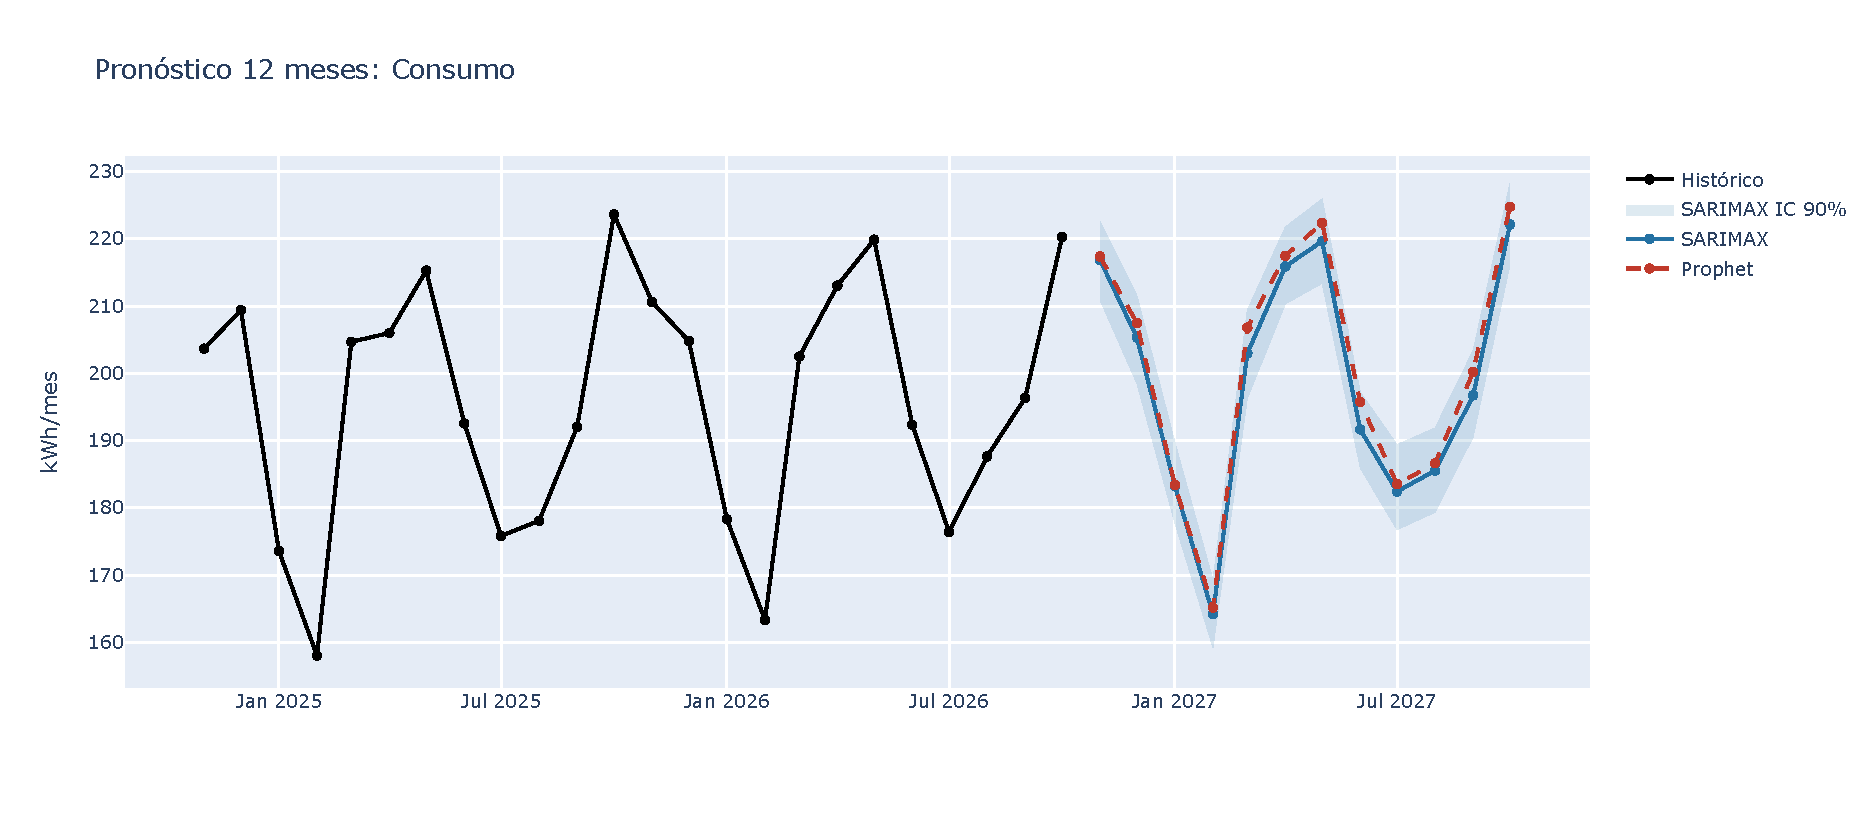
\includegraphics[width=\columnwidth]{figuras_gradio/ts_pronostico_consumo}\par}
{\par\centering\small\textbf{Figura~G.47:} Series temporales: pronostico consumo.\par\vspace{0.8em}}
{\par\centering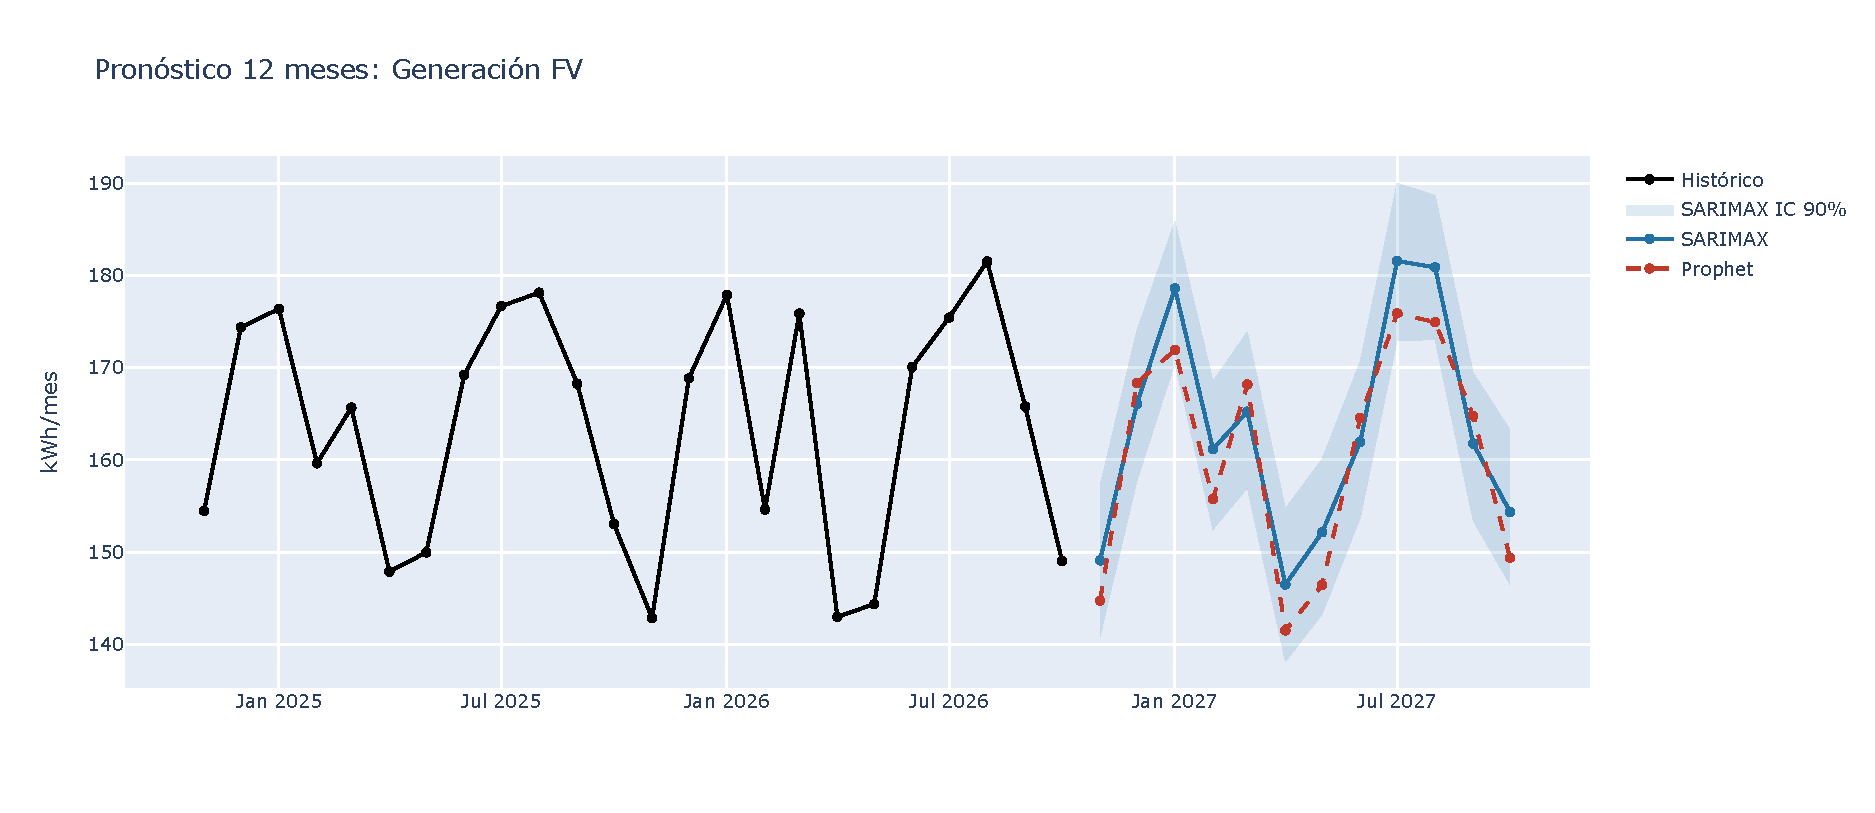
\includegraphics[width=\columnwidth]{figuras_gradio/ts_pronostico_generacion}\par}
{\par\centering\small\textbf{Figura~G.48:} Series temporales: pronostico generacion.\par\vspace{0.8em}}
{\par\centering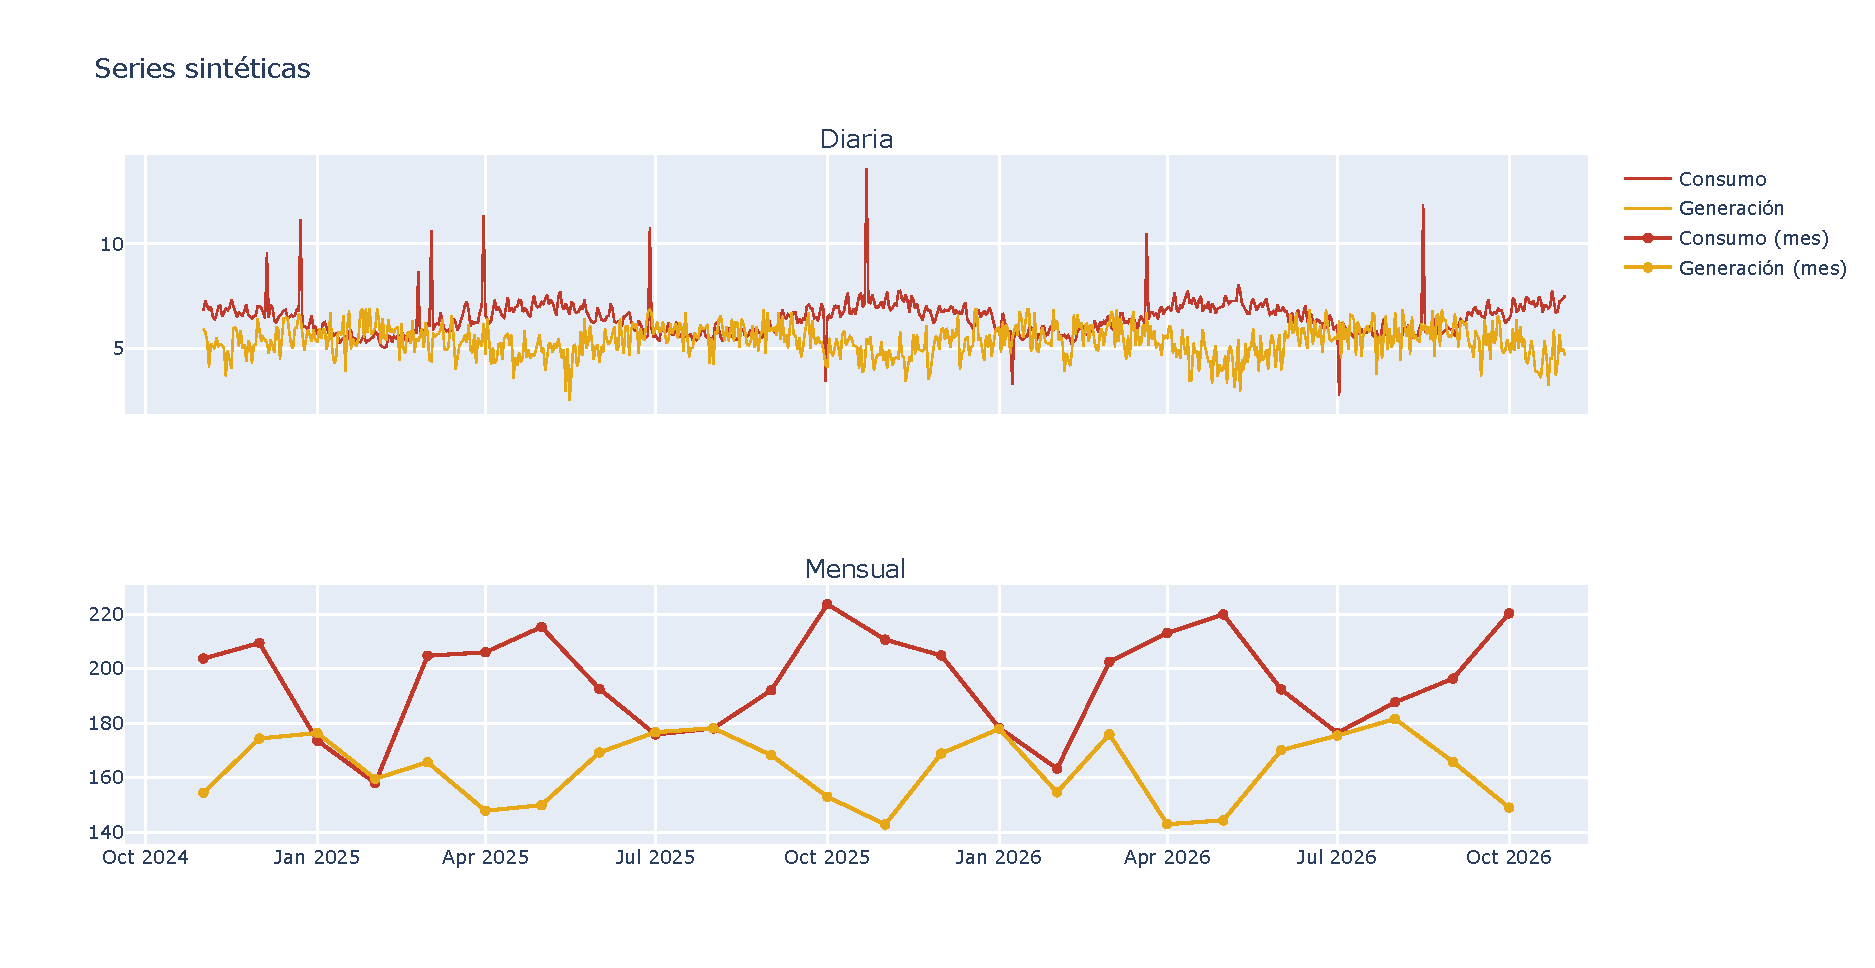
\includegraphics[width=\columnwidth]{figuras_gradio/ts_series}\par}
{\par\centering\small\textbf{Figura~G.49:} Series temporales: series.\par\vspace{0.8em}}
{\par\centering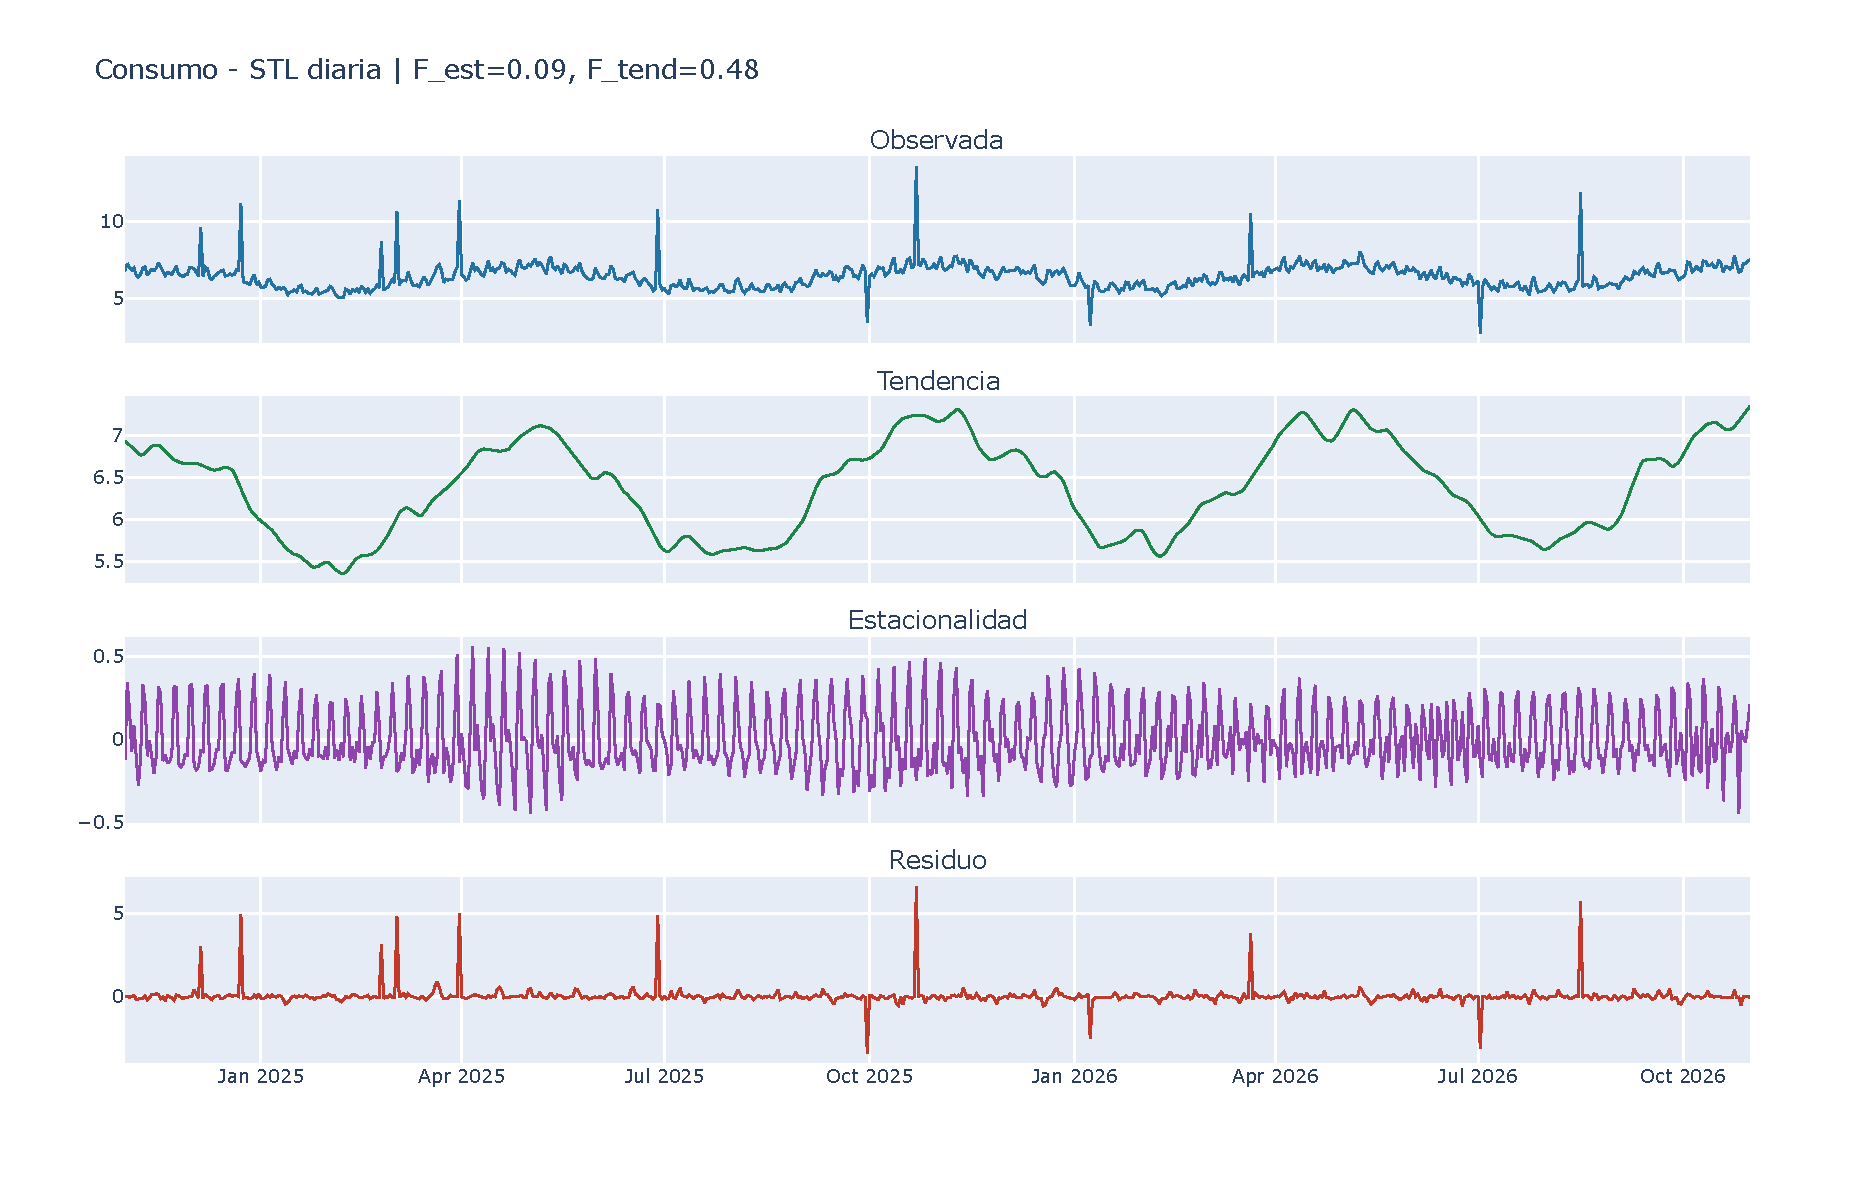
\includegraphics[width=\columnwidth]{figuras_gradio/ts_stl_consumo_diaria}\par}
{\par\centering\small\textbf{Figura~G.50:} Series temporales: stl consumo diaria.\par\vspace{0.8em}}
{\par\centering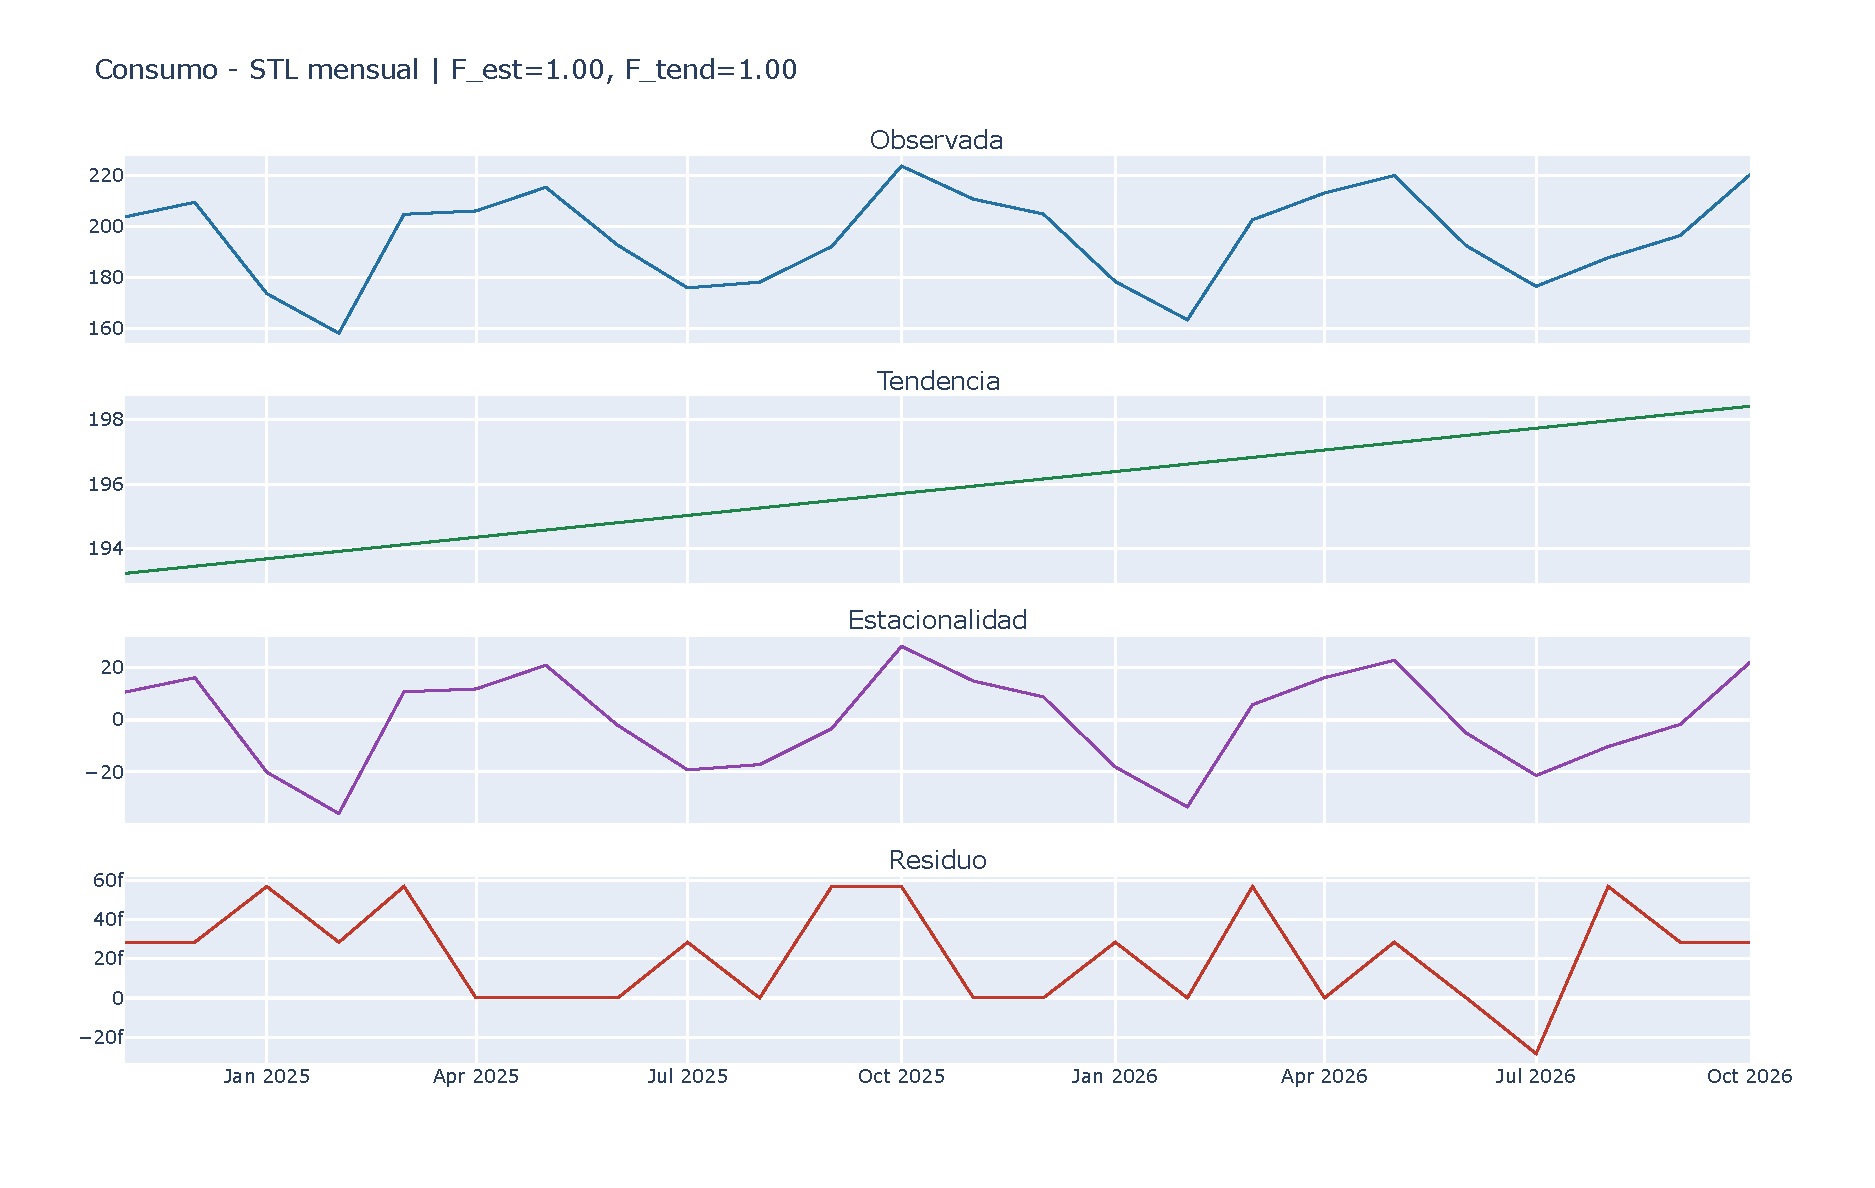
\includegraphics[width=\columnwidth]{figuras_gradio/ts_stl_consumo_mensual}\par}
{\par\centering\small\textbf{Figura~G.51:} Series temporales: stl consumo mensual.\par\vspace{0.8em}}
{\par\centering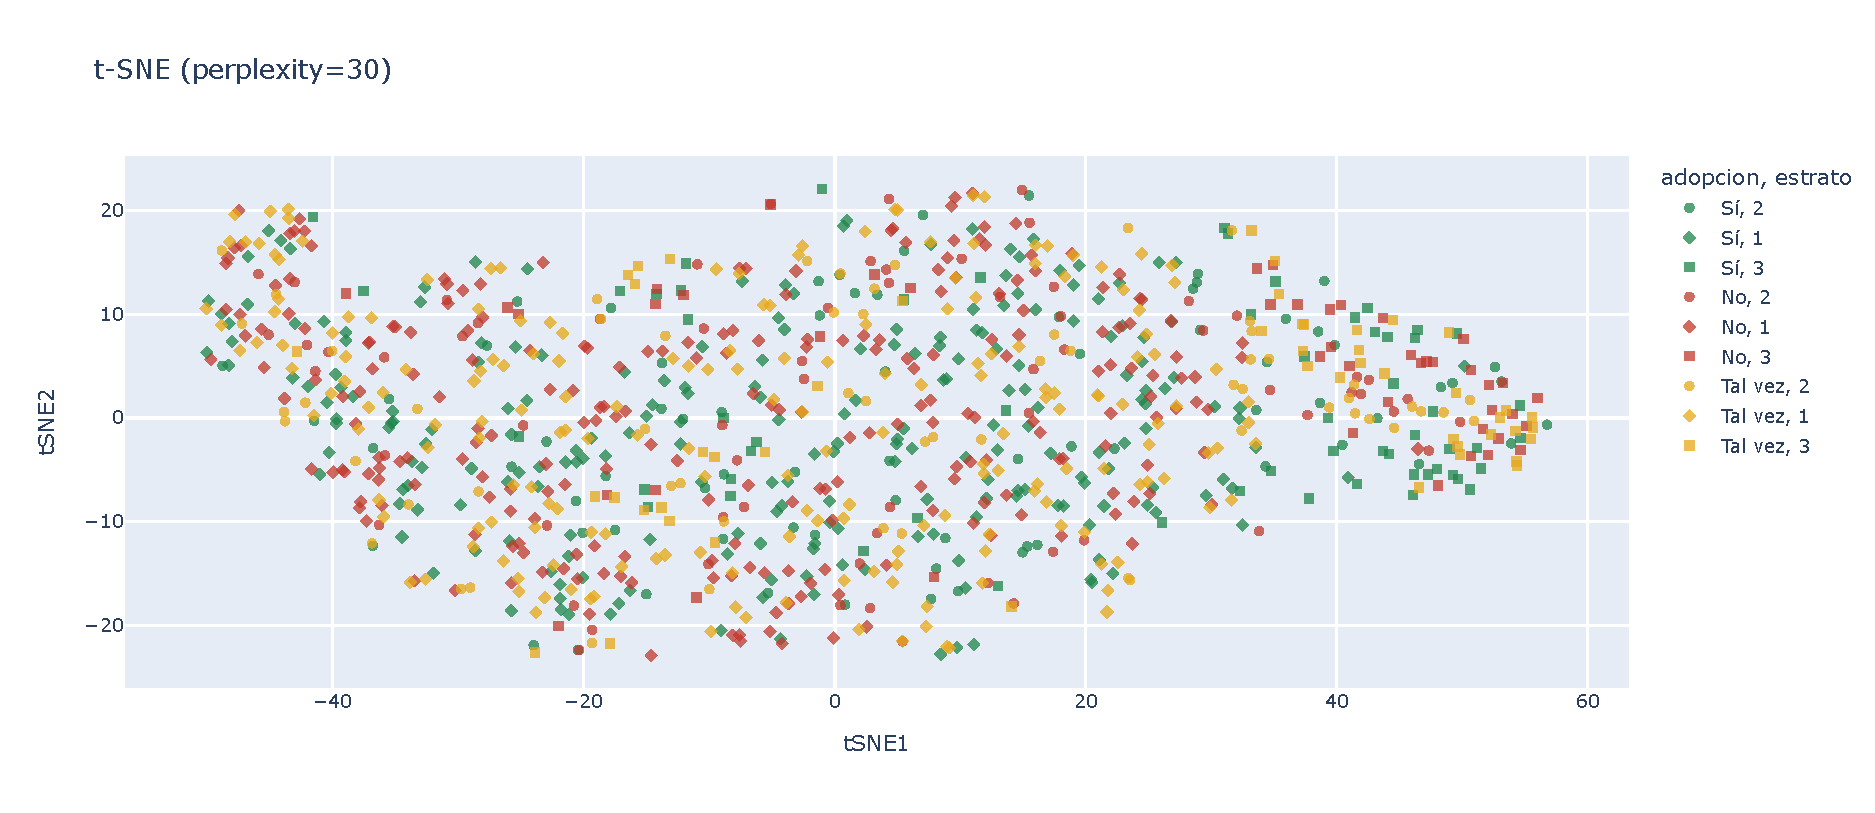
\includegraphics[width=\columnwidth]{figuras_gradio/tsne_2d}\par}
{\par\centering\small\textbf{Figura~G.52:} T-sne: 2d.\par\vspace{0.8em}}
\section{Anexos del documento original}
\subsection{Anexo D: encuesta propuesta}
\item ¿Cuántas personas habitan en su hogar?
\item ¿Cuál es el estrato socioeconómico de su vivienda?
\item ¿Cuál es el valor promedio mensual de su factura de energía?
\item ¿Ha considerado instalar paneles solares en su hogar?
\item ¿Conoce los incentivos de la Ley 1715 de 2014?
\item ¿Estaría dispuesto a participar en una comunidad energética?
\item ¿Cuenta con conexión a Internet en su hogar?
\item ¿Qué barreras identifica para instalar paneles solares?
\subsection{Anexo E: glosario}
\item[AGRC] Autogeneración Colectiva
\item[CREG] Comisión de Regulación de Energía y Gas
\item[DANE] Departamento Administrativo Nacional de Estadística
\item[DER] Recursos Energéticos Distribuidos
\item[FENOGE] Fondo de Energías No Convencionales y Gestión Eficiente de la Energía
\item[FNCER] Fuentes No Convencionales de Energía Renovable
\item[FONENERGIA] Fondo Único de Soluciones Energéticas
\item[GDC] Generación Distribuida Colectiva
\item[GEI] Gases de Efecto Invernadero
\item[IA] Inteligencia Artificial
\item[IDEAM] Instituto de Hidrología, Meteorología y Estudios Ambientales
\item[IPSE] Instituto de Planificación y Promoción de Soluciones Energéticas
\item[MME] Ministerio de Minas y Energía
\item[NBI] Necesidades Básicas Insatisfechas
\item[ODS] Objetivos de Desarrollo Sostenible
\item[PND] Plan Nacional de Desarrollo
\item[PROURE] Programa de Uso Racional y Eficiente de la Energía
\item[RAEE] Residuos de Aparatos Eléctricos y Electrónicos
\item[UPME] Unidad de Planeación Minero-Energética
\item[URE] Uso Racional y Eficiente de la Energía
\subsection{Anexo F: lista de verificación de coherencia}
\item ¿Se citan todas las normas suministradas en los PDF?
\item ¿Se identifican los artículos clave de cada norma?
\item ¿Se analizan las tensiones y derogatorias entre normas?
\item ¿Se evidencia el potencial solar de Popayán?
\item ¿Se caracteriza socioeconómicamente el territorio?
\item ¿Se identifican los actores relevantes?
\item ¿Se describen las brechas y necesidades?
\item ¿Se articula el mapa territorial con la matriz normativa?
\item ¿Se formula una pregunta orientadora clara y delimitada?
\item ¿Se justifica social, económica, ambiental y normativamente el proyecto?
\item ¿Se delimita temporal, espacial, conceptual y poblacionalmente el problema?
\item ¿Se proponen objetivos general y específicos coherentes?
\item ¿Se describe la metodología mixta?
\item ¿Se identifican los impactos y resultados esperados?
\item ¿Se incluyen indicadores de seguimiento?
\item ¿Se respeta el enfoque diferencial e interseccional?
\item ¿Se integra la IA y la economía circular?
\item ¿Se articula con los ODS y las NDC?
\item ¿Se usan citas en APA 7?
\item ¿Se incluyen anexos y glosario?
\section{Código fuente y reproducibilidad}
El código completo se conserva en el repositorio. La Tabla~\ref{tab:codigo} enumera los archivos ejecutables; el Listado~\ref{lst:pipeline} contiene íntegramente el pipeline Python.
\begin{table}[p]
\caption{Archivos de código fuente}
\label{tab:codigo}
\centering\footnotesize
\begin{tabular}{@{}lr@{}}
\toprule
Archivo & Líneas \\
\midrule
modulos/07-proyecto-integrador/notebooks/proyecto.ipynb & 4 celdas (432, 1878, 103, 15 líneas) \\
modulos/07-proyecto-integrador/export\_colab/proyecto.py & 2441 \\
modulos/07-proyecto-integrador/sitio-web/js/app.js & 986 \\
modulos/07-proyecto-integrador/sitio-web/js/solarnet.js & 160 \\
modulos/07-proyecto-integrador/sitio-web/js/herramientas.js & 150 \\
documento/ieee/generar\_figuras.py & 56 \\
\bottomrule
\end{tabular}
\end{table}
\begin{verbatim}
\end{verbatim}
A continuación se reproducen íntegramente los archivos ejecutables del proyecto.
\lstinputlisting[caption={Pipeline completo (proyecto.py)},label={lst:pipeline}]{../../modulos/07-proyecto-integrador/export_colab/proyecto.py}
\lstinputlisting[caption={Controlador web (app.js)}]{../../modulos/07-proyecto-integrador/sitio-web/js/app.js}
\lstinputlisting[caption={Red neuronal JavaScript (solarnet.js)}]{../../modulos/07-proyecto-integrador/sitio-web/js/solarnet.js}
\lstinputlisting[caption={Utilidades (herramientas.js)}]{../../modulos/07-proyecto-integrador/sitio-web/js/herramientas.js}
Las instrucciones de ejecución están en \texttt{documento/ieee/README.md}.
